\documentclass[review]{elsarticle}
%%%%%%%%%%%%%%%%%%%%%%%%%%%
\usepackage{pgfplots}
\pgfplotsset{compat=newest}
%% the following commands are needed for some matlab2tikz features
\usetikzlibrary{plotmarks}
\usetikzlibrary{arrows.meta}
\usepgfplotslibrary{patchplots}
\usepackage{grffile}
\usepackage{amsmath}
\pgfplotsset{ % Here we specify options for all figures in the document
	compat=1.8, % Which version of pgfplots do we want to use?
	legend style = {font=\small\sffamily}, % Legends in a sans-serif font
	label style = {font=\small\sffamily} % Labels in a sans-serif font
}
%% you may also want the following commands
%\pgfplotsset{plot coordinates/math parser=false}
%\newlength\figureheight
%\newlength\figurewidth
%%%%%%%%%%%%%%%%%%%%%%%%%%%
\usepackage{graphicx}
\usepackage{subcaption}
\captionsetup[subfigure]{% changed <<<<<<<<<<<<<<<<
	singlelinecheck = false,
	justification=raggedright, 
	margin = {-3ex, 0mm}, % make margin font size dependent
	position=top
}

\usepackage{lineno}
\usepackage{makecell}
\usepackage[hidelinks]{hyperref}
\hypersetup{
    colorlinks,
    linkcolor={blue!50!black},
    citecolor={blue!50!black},
    urlcolor={blue!50!black}
}
%\modulolinenumbers[5]
\usepackage{booktabs}
\journal{International Journal of Heat and Fluid Flow}

%%%%%%%%%%%%%%%%%%%%%%%
%% Elsevier bibliography styles
%%%%%%%%%%%%%%%%%%%%%%%


%% `Elsevier LaTeX' style
\bibliographystyle{elsarticle-num}
%%%%%%%%%%%%%%%%%%%%%%%

\usepackage{xcolor}
\usepackage{float}
\usepackage{amsmath}

\usepackage{setspace}
\biboptions{sort&compress}
\setlength{\bibsep}{4pt}

\setlength{\abovecaptionskip}{-2pt plus 0pt minus 0pt}
\setlength{\belowcaptionskip}{2pt plus 0pt minus 0pt}

\newcommand{\ave}[1]{\left<{#1}\right>}

\begin{document}
\newlength\figureheight
\newlength\figurewidth
\begin{frontmatter}

\title{Critical Assessment of the Lattice Boltzmann Method for Cavitation Modelling based on Single Bubble Dynamics}
%% or include affiliations in footnotes:
\author[address_1]{Xin Xiong}
\author[address_1]{Tom-Robin Teschner\corref{mycorrespondingauthor}}
\cortext[mycorrespondingauthor]{Corresponding author}
\ead{tom.teschner@cranfield.ac.uk}
\author[address_1]{Irene Moulitsas}
\author[address_1]{Tam\'{a}s Istv\'{a}n J\'{o}zsa}


\address[address_1] { Centre for Computational Engineering Sciences, Cranfield University, Cranfield MK43 0AL, UK.}

\begin{abstract}
Cavitation, a phenomenon with both detrimental and advantageous implications, is contingent upon its method of application. The simulation of cavitation bubbles serves as a crucial means to enhance our understanding. The Lattice Boltzmann Method (LBM) has emerged as a widely employed technique for simulating bubble dynamics, with the Shan-Chen model standing out due to its simplicity and popularity. In the validation of LBM results, the Rayleigh-Plesset (R-P) equation is commonly employed. However, the literature often lacks a comprehensive examination of the influence of boundary conditions, initial conditions, and bubble radius in this validation process.
This article elucidates that in the validation of single bubble dynamics, careful consideration must be given to the impact of domain sizes, the initial conditions of the model, and the radius of the bubble. Our findings reveal that an increase in bubble radius results in heightened resolution, consequently extending the iterations required for the difference between LBM and R-P to reach 5\%. This 5\% refers to the point where the difference in bubble radius calculated by R-P and LBM methods reaches a 5\% discrepancy after a certain number of iterations. Additionally, varying the domain size while maintaining parameters ($R_{\infty}$) in R-P equation unchanged, results in disparate outcomes. Moreover, the initial conditions derived from LBM and implemented in the R-P equation significantly affect the predictive accuracy of the R-P equation concerning bubble evolution.
In contrast to existing literature that predominantly presents results with a singular domain size and initial condition, our research emphasizes the critical need to meticulously investigate the effects of domain size and to thoughtfully choose initial conditions informed by the LBM. We assert that the simulation of a single bubble based on LBM is not a straightforward process but demands thorough consideration.
\end{abstract}

\begin{keyword}
Lattice Boltzmann Simulation, Rayleigh-Plesset Equation, Single Bubble
\MSC[2010] 76D55
\end{keyword}


\end{frontmatter}

\linenumbers

%%%%%%%%%%%%%%%%%%%%%%%%%%%%%%%%%%%%%%%%%%%%%%%%%%%%%%%%%%%%%%%%%%%%%%
\section{Introduction}
Cavitation is a phenomenon that involves the transition from liquid to vapour due to a decrease in pressure, leading to the formation of vapour bubbles within the liquid. This phenomenon occurs in many hydrodynamic machines, where the collapse of cavitation bubbles can generate high pressure and high temperature, resulting in noise, vibration, and erosion. However, cavitation can be leveraged to enhance heat transfer and for applications such as drilling petroleum wells, where micro-jets induced by the collapse of bubbles play a crucial role \cite{peng2019simulation}.

Numerous numerical attempts have been made to simulate cavitation bubbles using traditional macroscopic methods based on the Navier-Stokes equation \cite{ogloblina2018simulation,shang2022investigation,koch2016numerical}. In particular, the Shan-Chen model has gained popularity for its simplicity in simulating bubble dynamics. This model employs a potential to mimic the interaction between particles, adding force to the velocity to trigger phase separation \cite{yuan2021modelling}. For instance, there are numerous articles that focus on studying a single bubble near a solid wall based on the Shan-Chen model \cite{liu2021study,yxl2020numerical,mao2018study}. Furthermore, simulations of a bubble near a concave wall  and a bubble near a solid particle \cite{peng2020simulation} have also been conducted. The advantages of the Shan-Chen model include its ability to easily incorporate the equation of state and facilitate the automatic separation of phases and components.

In articles studying bubble dynamics based on the Shan-Chen model, the validation of bubble growth or collapse was conducted by comparing the Rayleigh-Plesset (R-P) equation with Lattice Boltzmann Method (LBM) simulation results. Shi et al. \cite{shi2020numerical} compared the R-P equation with LBM simulation results for a bubble radius of 20, focusing on growth and collapse. The simulation domain size was 2000x2000x1000, but the article did not provide a detailed analysis of the grid convergence study. Ezzatneshan and Vaseghnia \cite{ezzatneshan2021dynamics} also validated LBM results for the same radius against the R-P equation under different pressures, determining the critical pressure for bubble growth or collapse. However, their study only considers a radius of 15, and the influence of different radii was not explored. Figure analysis reveals some discrepancies, especially at the end under certain pressure differences, possibly due to insufficient resolution at small radii.

Peng et al. \cite{peng2019simulation} compared LBM results with variable boundary pressure against the relevant R-P equation, demonstrating good agreement with slight deviations at the beginning. This suggests that initial conditions significantly influence the results. In another study, Peng et al. \cite{peng2018single} investigated LBM results with different pressure differences and radii against the R-P equation. While results were satisfactory in certain iterations, small deviations were observed. Unfortunately, their study lacked a detailed analysis of initial conditions and domain size.

Emphasizing these findings, it becomes evident that there is a notable research gap in the existing literature. Specifically, there is a lack of comprehensive analyses regarding the influence of different bubble radii, and detailed investigations into the effects of initial conditions and domain size on LBM simulations in the context of bubble dynamics based on the Shan-Chen model.

The primary aim of this article is to undertake a critical assessment of the Lattice Boltzmann method concerning its application to single bubble dynamics and, in turn, to establish a foundational framework for the simulation of bubble clusters. To realize this aim, the article is structured as follows:

In section two, the mathematical formulations governing the simulation, encompassing relevant equations, and the explication of the problem statement and setup are delineated. Section three delves into an in-depth presentation and discussion of results, focusing on the discernible impacts of the initial conditions, boundary conditions, and the radius of the bubble. The final section serves as the conclusion, synthesizing key insights and implications derived from the critical assessment presented in the preceding sections. 

%%%%%%%%%%%%%%%%%%%%%%%%%%%%%%%%%%%%%%%%%%%%%%%%%%%%%%%%%%%%%%%%%%%%%%
\section{Methodology}

\subsection{Equations of the Simulation}
In this article, a two-dimensional $D2Q9$ model was implemented based on the Shan-Chen multiphase model. The additional force was considered through the velocity shifting method by modifying the equilibrium velocity, without any alteration to the Lattice Boltzmann Equation, as expressed in \cite{kruger2017lattice}
\begin{linenomath*}
\begin{equation}
	f_i\left(x+e_i \Delta t, t+\Delta t\right)-f_i(x, t)=-\frac{1}{\tau}\left[f_i(x, t)-f_i^{e q}(x, t)\right],
\end{equation}
\end{linenomath*}
where represents one of the nine directions, $f$ is the density distribution function, $x$, $t$ are the coordinate in space and time, $\Delta t$ is the time step, $e_i$ is the unit vector direction of the lattice, $\tau$ is the relaxation time and $f^{eq}$ is the equilibrium density distribution function.
The equilibrium density distribution function can be expressed as \cite{mohamad2011lattice}
\begin{linenomath*}
\begin{equation}
	f_i^{e q}(x, t)=\omega_i \rho(x)\left[1+\frac{3 e_i \cdot u}{c^2}+\frac{9\left(e_i \cdot u\right)^2}{2 c^4}-\frac{3 u^2}{2 c^2}\right],
\end{equation}
\end{linenomath*}
where the weights $\omega_i$ are equal to 4/9 for $i=0$, 1/9 for $i=1$ to $4$, and 1/36 for $i=5$ to $9$; $c$ is the lattice speed; $\rho$ is the density; and $u$ is the macro velocity vector. The term $e_i$ represents the vector quantity of unit direction of lattice speed. According to Shan and Chen \cite{shan1993lattice}, the additional force can be expressed as
\begin{linenomath*}
\begin{equation}
	F(x, t)=-G \psi(x, t) \sum_{i=0}^8 \omega_i \psi\left(x+e_i t, t\right) e_i,
\end{equation}
\end{linenomath*}
where $G$ denotes the interaction strength between particles, and $\psi$ represents the effective density. Additionally, the velocity shifting method was implemented to enhance stability, as referenced in \cite{kruger2017lattice}
\begin{linenomath*}
\begin{equation}
	u^{\mathrm{eq}}=\frac{1}{\rho}\left(\sum_i f_i c_i+\tau F\right),
\end{equation}
\end{linenomath*}
where $F$ represents the Shan-Chen force vector and $u^{eq}$ is the vector of equilibrium velocity. Furthermore, the (Carnahan-Starling) C-S Equation of State (EOS) is incorporated through modifications to the effective density \cite{shi2020numerical}
\begin{linenomath*}
\begin{equation}
	\psi=\sqrt{\frac{2}{G c_s^2}\left(p-\rho c_s^2\right)},
\end{equation}
\end{linenomath*}
with different pressure $p$. In addition, $c_s$ is the speed of sound. The C-S equation of state \cite{peng2019simulation}
\begin{linenomath*}
\begin{equation}
	P=\rho R T \frac{1+b \rho / 4+(b \rho / 4)^2-(b \rho / 4)^3}{(1-b \rho / 4)^3}-a \rho^2,
\end{equation}
\end{linenomath*}
is implemented in this article with $a= 0.4963R^2T_c^2/P_c$,$b=0.18727RT_c^2/P_c$. Where $ a= 1, b= 4, R= 1$, the
critical temperature, pressure and density are $T_c = 0.09433, P_c=0.00441644$, and $\rho_c= 0.13044$. In this article, $T/T_c$ is set to 0.75, and the simulation is assumed to be isothermal.

Additionally, this article focuses on a two-dimensional LBM simulation within a square domain. Consequently, the associated R-P equation is derived using a cylindrical coordinate system, based on the principles of continuity and momentum equations, ultimately being formulated as \cite{brennen2014cavitation}
\begin{linenomath*}
\begin{equation}
	\ddot{R}=\left(\frac{P_v-P_{\infty}}{\rho_l}-\frac{\sigma}{\rho_l R} -\frac{2 \nu}{R} \dot{R}+\frac{1-\left(\frac{R}{R \infty}\right)^2}{2} \dot{R}^2-\ln \frac{R_{\infty}}{R} \dot{R}^2\right)/\left(\ln \frac{R_{\infty}}{R} \cdot R\right),
\label{equ:r-p}
\end{equation}
\end{linenomath*}
where $R$, $R_{\infty}$, $\dot{R}$, $\ddot{R}$, $\sigma$, $\nu$, $\rho_l$, $P_v$, $P_{\infty}$ are radius, the distance between the centre of the domain and the boundary, first derivative of the radius, second derivative of the radius, the surface tension, kinematic viscosity, liquid density, vapour pressure and pressure on the boundary. 
\subsection{Problem statement and the test cases}
In this article, two sets of problems are simulated based on the Shan-Chen model. One is a bubble in a square domain as in \ref{fig:schematic}(a); another is a flat interface simulation as sketched in Figure \ref{fig:schematic}(b). 
\begin{figure}[htp]
	\centering
	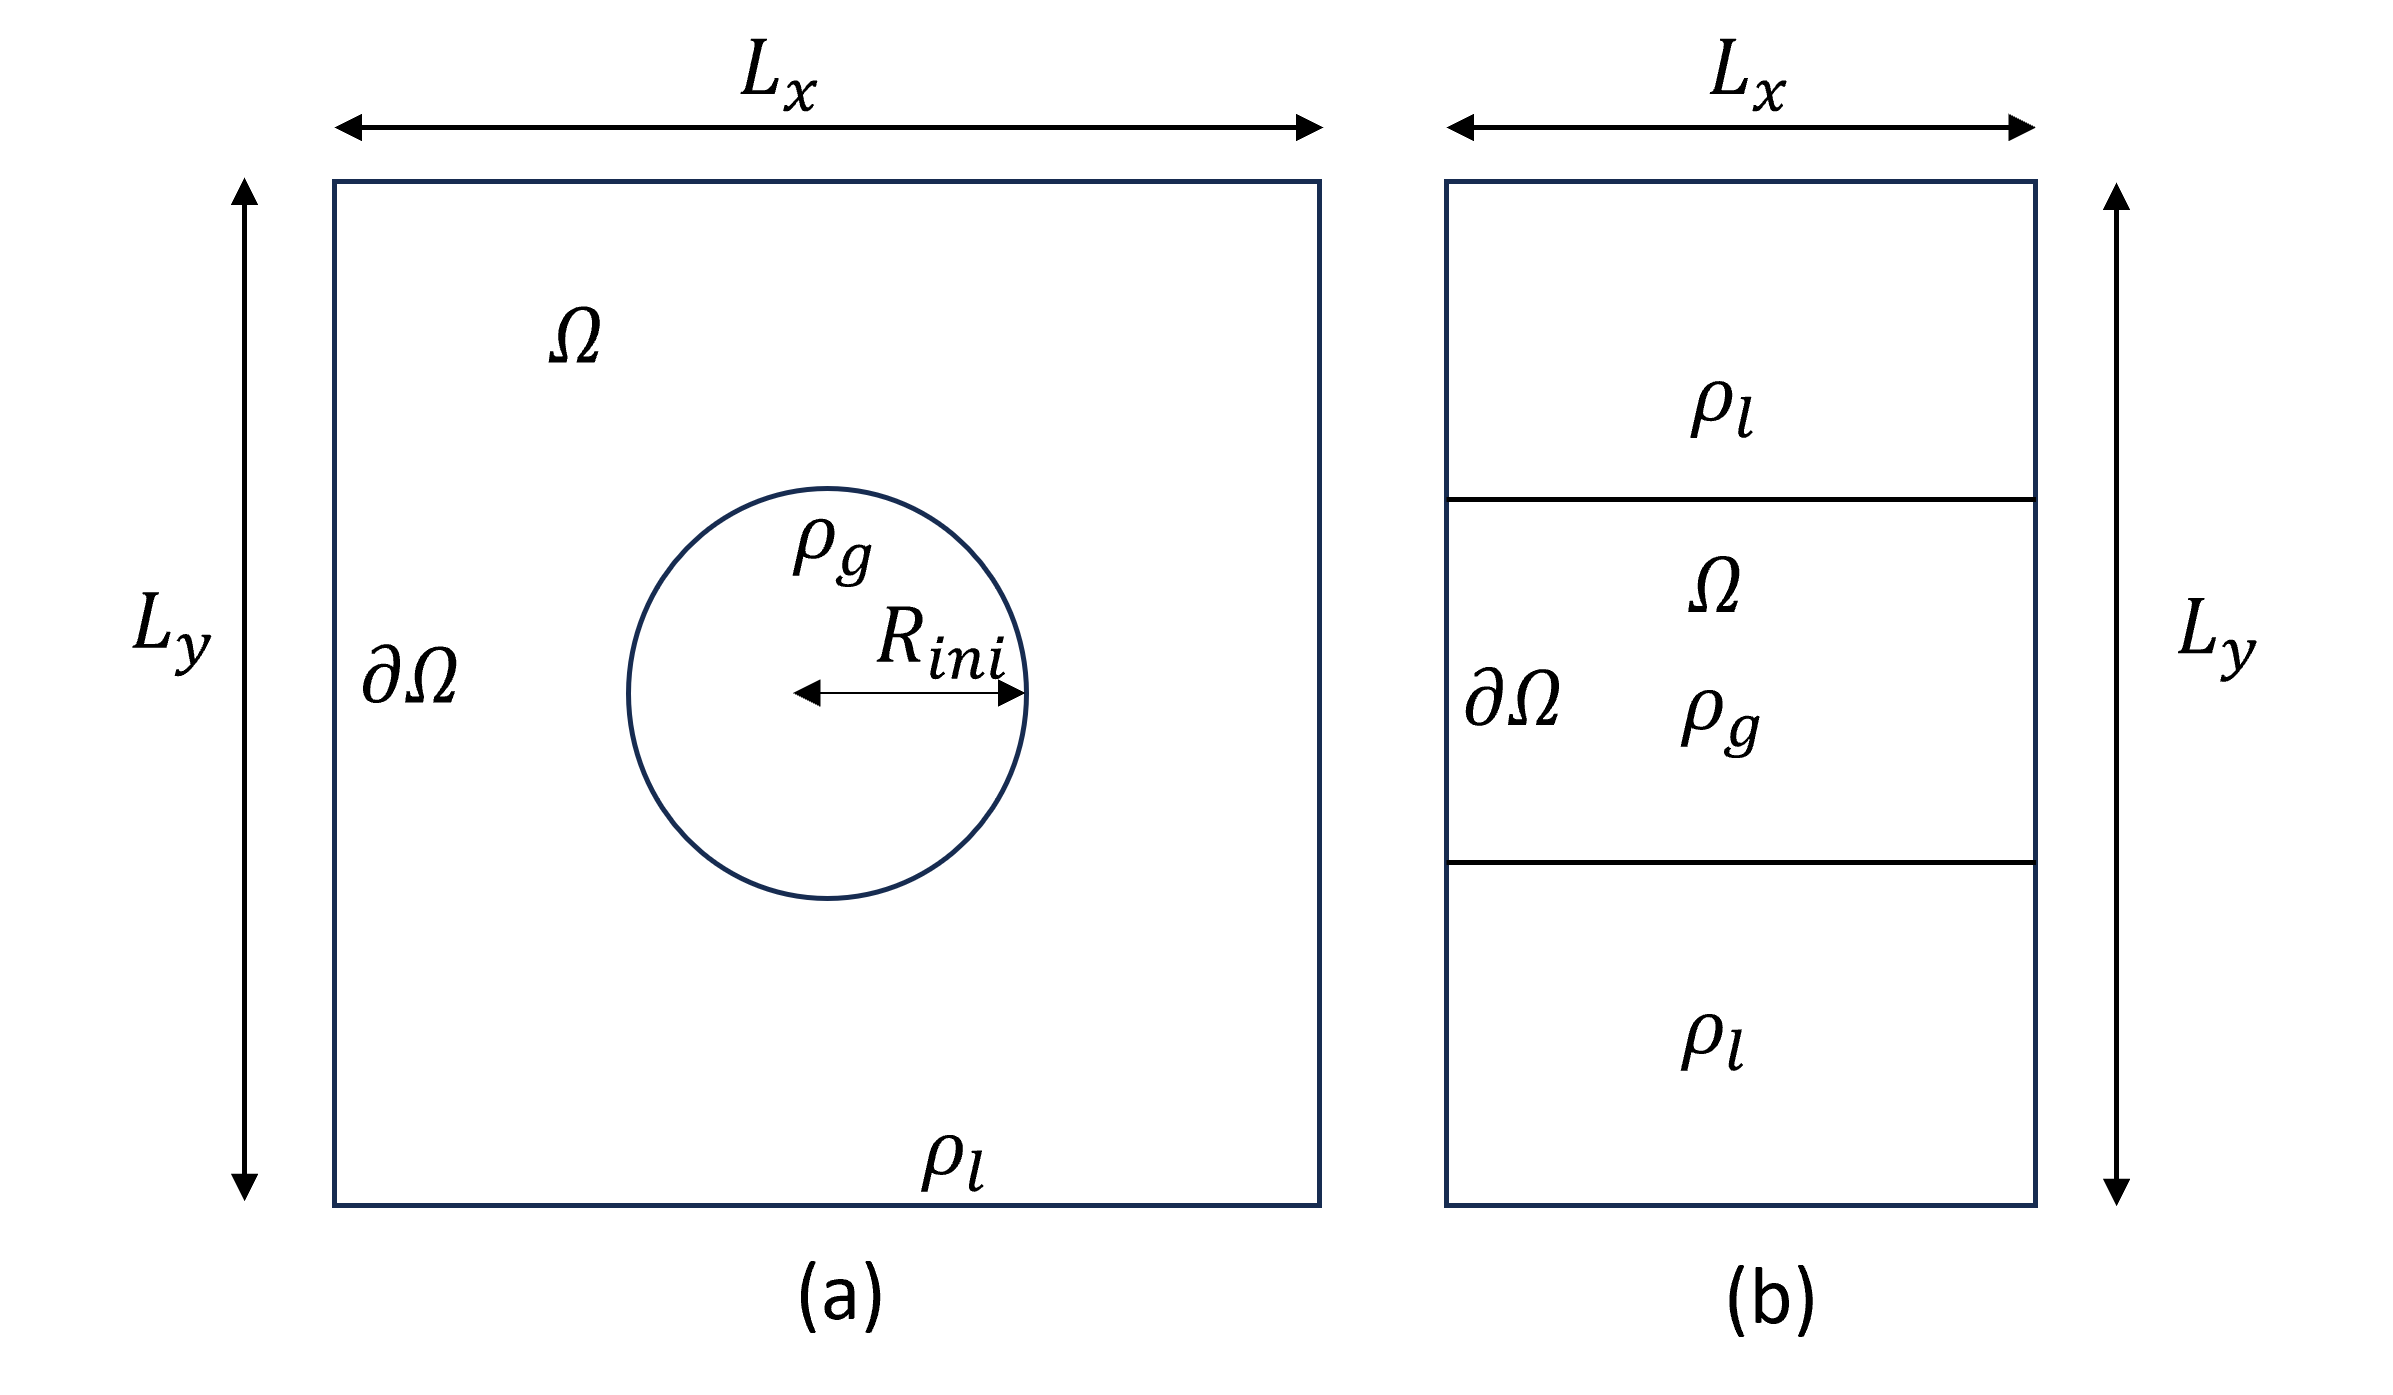
\includegraphics[width=0.6\textwidth]{schematic.png}
	\caption{Problem statement of the simulation (a) bubble simulation (b) flat interface simulation. The coordinate origin is placed in the centre of the domain in both cases}
	\label{fig:schematic}
\end{figure}
In both cases, the C-S EOS is implemented. The interaction strength $G$ cannot affect the results \cite{shi2020numerical}, since it will be eliminated during the calculation; therefore, it was set to -1 for simplicity. Numerical tests showed that a relaxation factor of $\omega=1$ provided acceptable stability and is chosen throughout this study
\subsubsection{Flat interface case}
In the flat interface case, the width of the domain $\Omega$, $L_x$, is set to 20 (lattice length unit) l.u., and the height, $L_y$, to 200 l.u. In the middle of the domain, it is set as gas phase with an initial density $\rho_g$ and pressure $p_g$ given. At the top and the bottom, the liquid phase is present, where initial pressure $p_l$ and density $\rho_l$ are implemented. To eliminate the effect of the boundary $\partial \Omega$, a periodic boundary condition is set in the flat interface simulation. In addition, the interface is also smoothed in the flat interface simulation (the width of interface is denoted as $W$ in equation \ref{equ:smooth1}) according to Huang et al. \cite{huang2019thermodynamic} as
\begin{linenomath*}
\begin{equation}
	\begin{aligned}
		\rho(y)= & \rho_v+\frac{\rho_l-\rho_v}{2} \times \operatorname{abs}\left\{\tanh \left[\frac{2(y-50)}{W}\right]\right. \\
		& \left.-\tanh \left[\frac{2(y-150)}{W}\right]\right\},
	\end{aligned}
\label{equ:smooth1}
\end{equation}
\end{linenomath*}
After reaching the equilibrium state, the densities of liquid and gas were recorded against each reduced temperature. The equilibrium state is defined as the condition when the change in density between two iterations is less than $10^{-4}$.
\subsubsection{Bubble case}
In the bubble simulation case, $L_x$ and $L_y$ are equal, forming a square domain in region $\Omega$. Inside the bubble, the gas pressure $p_g$ and the density of gas $\rho_g$ are set. Different bubble radii $R$ are set. In the bubble simulation, there are two minor problems with two boundary conditions $\partial \Omega$: one is a periodic boundary condition for Laplace law validation, and the other is the constant pressure $p_l$ and density $\rho_l$ boundary condition for R-P equation validation. In the Laplace law validation case, three radii of 20, 25, 30 with a domain size of 100 were set. In both bubble cases, an initial smooth interface was implemented on the bubble interface with 5 lattices for better stability according to Peng et al. \cite{peng2019simulation}.
\begin{linenomath*}
	\begin{align}
		\rho(x,y)&=\frac{\rho_{\text{liquid}}+\rho_{\text{vapor}}}{2}+\frac{\rho_{\text{liquid}}-\rho_{\text{vapor}}}{2} \cdot\notag \\
		&\tanh\left(\frac{2(\sqrt{(x-x_{0})^{2}+(y-y_{0})^{2}}-R_{init})}{5}\right)
	\end{align}
	\label{equ:smooth2}
\end{linenomath*}

In the constant pressure boundary condition case, a bounce-back boundary condition is set to validate the R-P equation. For stability reasons, the reduced temperature was chosen to be 0.75. The equilibrium densities of the liquid and gas, taken from Maxwell's area construction based on the C-S EOS, are 0.33 and 0.011, respectively. To trigger the growth and collapse of the bubble, densities different from the equilibrium density of the liquid on the boundary were implemented, which are 0.34 for collapse and 0.31 for growth, respectively. Furthermore, 1000 time steps were simulated for a sufficiently long time for bubble growth and collapse. The domain size for the bubble simulation is set to be square, including 100 (l.u), 200 (l.u), 400 (l.u) and 1000 (l.u).

The calculation of the radius is predicated on the average density of the liquid and gas at the brink of the bubble. The density of the liquid is computed as an average at a significant distance from the bubble, whereas the gas density is calculated as an average within the bubble, incorporating four cells at its centre. The justification for this approach stems from the premise that the density of a bubble remains nearly constant, both internally and externally. Averaging across four cells further mitigates issues related to small bubble sizes by ensuring that the calculation of gas density remains as accurate as possible. Furthermore, the pressure is averaged following the same strategy employed for density, and this averaged pressure is then incorporated into the R-P equation. Testing has demonstrated that the pressure remains relatively stable, indicating that variations in pressure averaging strategies—ranging from averaging across the entire bubble to averaging at the bubble's periphery—do not significantly impact the results.

In LBM simulations, the setup is an Initial Value Problem (IVP) where initial conditions like bubble radius and liquid density are set, but it also involves Boundary Value Problem (BVP) aspects, requiring boundary values at $\partial \Omega$. Conversely, the R-P equation primarily treats the problem as an IVP with boundaries at infinity, specifying initial $R$ and  $\dot{R}$ , underlining minimal distant boundary effects.

To analyse the impact of domain size, radius, and boundary condition in the bubble case with constant pressure boundary condition, different cases were carried out as follows in the table \ref{tab:cases}.
% Table generated by Excel2LaTeX from sheet 'Sheet1'
\begin{table}[htbp]
	\centering
	\caption{Different Cases}
	\begin{tabular}{llrr}
		\toprule
		\toprule
		& domain size & \multicolumn{1}{l}{radius} & \multicolumn{1}{l}{density} \\
		\midrule
		case1-4 & 100 200 400 1000 & 20    & 0.31 \\
		\midrule
		case5-8 & 100 200 400 1000 & 20    & 0.34 \\
		\midrule
		case9-13 & 100 200 400 1000 & 25    & 0.31 \\
		\midrule
		case14-17 & 100 200 400 1000 & 25    & 0.34 \\
		\midrule
		case18-21 & 100 200 400 1000 & 30    & 0.31 \\
		\midrule
		case22-25 & 100 200 400 1000 & 30    & 0.34 \\
		\midrule
		case26-29 & 100 200 400 1000 & 35    & 0.31 \\
		\midrule
		case30-32 & 100 200 400 1000 & 35    & 0.34 \\
		\bottomrule
		\bottomrule
	\end{tabular}%
	\label{tab:cases}%
\end{table}%
As can be seen from Table \ref{tab:cases}, there are a total of 32 cases, with each radius subjected to two situations of growth and collapse, and each situation was carried out with four domain sizes ranging from 100 to 1000.   

\section{Results and Discussion}
\subsection{Laplace Law validation}
As stated before in the previous section, Laplace law validation was first performed with three initial radii. As can be seen from Figure \ref{fig:lap-maxwell}(a), the bubble gradually evolves to the equilibrium state with periodic boundary conditions. According to the literature \cite{porter2012multicomponent,liu2010modified,ezzatneshan2021dynamics}, during this validation, the Laplace Law can be expressed as
\begin{linenomath}
\begin{equation}
	p_c=p_b-p_s=\frac{\sigma}{R},
	\label{equ:lap}
\end{equation}
\end{linenomath}
where $\sigma$ is the surface tension, $R$ is the radius, and $p_c, p_b, p_s$ are the capillary pressure, bubble, and suspending fluid pressure, respectively. As can be seen from Figure \ref{fig:lap-maxwell} (b), the results from LBM are in quite good agreement with the Laplace law. The slope is the surface tension as expressed in Equation \ref{equ:lap}.

In addition, to validate the thermodynamic consistency, the Maxwell Area construction was validated. As stated in the last section, the equilibrium densities are extracted at each temperature. For simplicity, the reference data were digitized from Peng et al. \cite{peng2019simulation}. As can be seen from Figure \ref{fig:lap-maxwell}(c), the LBM results are quite close to the reference data, which validates our code for thermodynamic consistency.
\begin{figure}[htp!]
	% y-axis tick label width
	\pgfplotsset{yticklabel style={text width=1.4em,align=left}}
	\pgfplotsset{xticklabel style={text width=1em,align=left}}
		\centering
		\setlength\figureheight{1\textwidth}
		\setlength\figurewidth{0.8\textwidth}
		% This file was created by matlab2tikz.
%
%The latest updates can be retrieved from
%  http://www.mathworks.com/matlabcentral/fileexchange/22022-matlab2tikz-matlab2tikz
%where you can also make suggestions and rate matlab2tikz.
%
\definecolor{mycolor1}{rgb}{0.00000,0.44700,0.74100}%
\definecolor{mycolor2}{rgb}{0.85000,0.32500,0.09800}%
\definecolor{mycolor3}{rgb}{0.92900,0.69400,0.12500}%
%
\begin{tikzpicture}

\begin{axis}[%
width=0.969\figurewidth,
height=0.251\figureheight,
at={(0\figurewidth,0.749\figureheight)},
scale only axis,
xmin=0,
xmax=5000,
xlabel style={font=\color{white!15!black}},
xlabel={$t\, \mathrm{[t.u.^{-1}]}$},
ymin=-5.66593078238712,
ymax=6.43104796808603,
ylabel style={font=\color{white!15!black}},
ylabel={$(\frac{1}{R} - \overline{R}) / R_{std}$},
axis background/.style={fill=white},
legend style={at={(0.97,0.03)}, anchor=south east, legend columns=3, legend cell align=left, align=left, draw=white!15!black}
]
\addplot [color=mycolor1, line width=1.0pt, forget plot]
  table[row sep=crcr]{%
1	2.7769080015284\\
2	2.52597184155931\\
3	2.11146533191712\\
4	1.65462296706543\\
5	1.20124444491269\\
6	0.780579992694583\\
7	0.403406009918964\\
8	0.0731863392848133\\
9	-0.212003376262874\\
10	-0.456781593656018\\
11	-0.66576676982659\\
12	-0.844347104528522\\
13	-0.99752592610474\\
14	-1.12953682007621\\
15	-1.24499824337488\\
16	-1.34660429587768\\
17	-1.43704907746164\\
18	-1.5178720737707\\
19	-1.59099764185984\\
20	-1.65758039596206\\
21	-1.71877495031037\\
22	-1.77535104772671\\
23	-1.82769355962209\\
24	-1.87695710022952\\
25	-1.92352654095998\\
26	-1.96740188181348\\
27	-2.00935286561199\\
28	-2.04976436376651\\
29	-2.08902124768806\\
30	-2.12673864596561\\
31	-2.16368630142118\\
32	-2.19947934264378\\
33	-2.23488751245537\\
34	-2.26991081085595\\
35	-2.30454923784556\\
36	-2.33880279342416\\
37	-2.37267147759175\\
38	-2.40615529034836\\
39	-2.43963910310497\\
40	-2.47312291586159\\
41	-2.50622185720722\\
42	-2.53932079855282\\
43	-2.57203486848745\\
44	-2.60474893842208\\
45	-2.63746300835667\\
46	-2.6701770782913\\
47	-2.70289114822593\\
48	-2.73522034674955\\
49	-2.76754954527316\\
50	-2.79987874379678\\
51	-2.83220794232043\\
52	-2.86453714084405\\
53	-2.89686633936767\\
54	-2.92881066648031\\
55	-2.96075499359292\\
56	-2.99308419211654\\
57	-3.02502851922918\\
58	-3.05697284634182\\
59	-3.08853230204345\\
60	-3.12047662915606\\
61	-3.1520360848577\\
62	-3.18359554055933\\
63	-3.21515499626096\\
64	-3.24671445196259\\
65	-3.27788903625325\\
66	-3.30867874913289\\
67	-3.33946846201251\\
68	-3.36987330348118\\
69	-3.40027814494982\\
70	-3.43029811500748\\
71	-3.45993321365413\\
72	-3.48956831230078\\
73	-3.51920341094744\\
74	-3.54883850959409\\
75	-3.57847360824074\\
76	-3.60887844970938\\
77	-3.64005303400004\\
78	-3.67238223252366\\
79	-3.70663578810225\\
80	-3.74242882932485\\
81	-3.7813008418354\\
82	-3.82286695422291\\
83	-3.86789690930937\\
84	-3.91677557850582\\
85	-3.97027270463419\\
86	-4.02800341628352\\
87	-4.0903525848648\\
88	-4.15655046755604\\
89	-4.22736680717919\\
90	-4.30164698950133\\
91	-4.37823640028945\\
92	-4.45713503954353\\
93	-4.53641855020862\\
94	-4.6149323180517\\
95	-4.6919066002508\\
96	-4.76541703975095\\
97	-4.83430902231915\\
98	-4.89704306231141\\
99	-4.95246454549479\\
100	-4.99980372904724\\
101	-5.03790599873579\\
102	-5.06638648314945\\
103	-5.08447543946623\\
104	-5.09255773909716\\
105	-5.09024851063117\\
106	-5.07754775406833\\
107	-5.05522521223058\\
108	-5.02366575652895\\
109	-4.98363912978541\\
110	-4.93591507482196\\
111	-4.88087846304962\\
112	-4.82006878011231\\
113	-4.75387089742107\\
114	-4.6834394292089\\
115	-4.60954411829777\\
116	-4.53333957892065\\
117	-4.45521068248856\\
118	-4.37631204323447\\
119	-4.2966436611584\\
120	-4.21774502190432\\
121	-4.13961612547223\\
122	-4.06302671468411\\
123	-3.98797678953998\\
124	-3.91523609286182\\
125	-3.84518949606065\\
126	-3.77745212772544\\
127	-3.71317860208918\\
128	-3.65159917632989\\
129	-3.59348359326957\\
130	-3.53844698149721\\
131	-3.48648934101281\\
132	-3.43838041463838\\
133	-3.39296558814091\\
134	-3.35101460434239\\
135	-3.31175772042084\\
136	-3.27557980778726\\
137	-3.24209599503065\\
138	-3.211306282151\\
139	-3.18244092632634\\
140	-3.15588479896766\\
141	-3.13125302866395\\
142	-3.10777587259322\\
143	-3.08583820216648\\
144	-3.06467027456171\\
145	-3.04427208977895\\
146	-3.02425877640719\\
147	-3.00424546303541\\
148	-2.98384727825265\\
149	-2.96306422205891\\
150	-2.94151142304315\\
151	-2.9188040097944\\
152	-2.89494198231269\\
153	-2.86992534059798\\
154	-2.8433692132393\\
155	-2.81527360023662\\
156	-2.78563850158997\\
157	-2.75407904588833\\
158	-2.7209801045427\\
159	-2.68595680614212\\
160	-2.64939402209753\\
161	-2.61090688099799\\
162	-2.57126512566546\\
163	-2.53046875609994\\
164	-2.48774802947944\\
165	-2.44425756003692\\
166	-2.39961247636144\\
167	-2.35381277845299\\
168	-2.3076282091335\\
169	-2.26028902558105\\
170	-2.21256497061763\\
171	-2.16445604424319\\
172	-2.11557737504674\\
173	-2.06669870585032\\
174	-2.01705029383188\\
175	-1.96740188181348\\
176	-1.91736859838406\\
177	-1.86695044354364\\
178	-1.81614741729224\\
179	-1.76495951962983\\
180	-1.71300187914543\\
181	-1.66027449583903\\
182	-1.60677736971066\\
183	-1.5521256293493\\
184	-1.49593440334394\\
185	-1.43858856310561\\
186	-1.3793183658123\\
187	-1.31773894005301\\
188	-1.25423515723877\\
189	-1.18803727454753\\
190	-1.11914529197932\\
191	-1.04717433812317\\
192	-0.971739541568046\\
193	-0.893225773724944\\
194	-0.810863291771909\\
195	-0.725036967119922\\
196	-0.634977056946943\\
197	-0.541453304075038\\
198	-0.443695965682167\\
199	-0.342089913179364\\
200	-0.236635146566575\\
201	-0.127331665843854\\
202	-0.0145643424221798\\
203	0.101666823698473\\
204	0.221361832518079\\
205	0.343750941214678\\
206	0.469219021199222\\
207	0.596996329649726\\
208	0.727082866566216\\
209	0.859093760537685\\
210	0.993029011564134\\
211	1.12811887682355\\
212	1.26397848490498\\
213	1.40060783580839\\
214	1.53762205812279\\
215	1.67502115184819\\
216	1.81165050275161\\
217	1.94789498224401\\
218	2.08336971891446\\
219	2.22731162662679\\
220	2.37895096255901\\
221	2.52635671297031\\
222	2.66875913503864\\
223	2.80654310017505\\
224	2.93970860837949\\
225	3.067870788241\\
226	3.19141451117056\\
227	3.3099549057572\\
228	3.42349197200089\\
229	3.53202570990162\\
230	3.63594099087041\\
231	3.73485294349625\\
232	3.82914643919017\\
233	3.91843660654113\\
234	4.00272344554915\\
235	4.08277669903622\\
236	4.15782662418034\\
237	4.22825809239252\\
238	4.29445597508376\\
239	4.35603540084302\\
240	4.41338124108138\\
241	4.46610862438776\\
242	4.51498729358418\\
243	4.55963237725966\\
244	4.60042874682519\\
245	4.63737640228075\\
246	4.67086021503737\\
247	4.70049531368405\\
248	4.72705144104273\\
249	4.75014372570245\\
250	4.77054191048522\\
251	4.78824599539101\\
252	4.80364085183082\\
253	4.81634160839369\\
254	4.82750287931256\\
255	4.83673979317645\\
256	4.84482209280735\\
257	4.85136490679428\\
258	4.85713797795922\\
259	4.86214130630214\\
260	4.86637489182311\\
261	4.87060847734405\\
262	4.87484206286501\\
263	4.87907564838595\\
264	4.8836941053179\\
265	4.88869743366085\\
266	4.89408563341478\\
267	4.9002435759907\\
268	4.90678638997762\\
269	4.91409894678656\\
270	4.92179637500645\\
271	4.93026354604836\\
272	4.93950045991225\\
273	4.94950711659813\\
274	4.95951377328403\\
275	4.9702901727919\\
276	4.98145144371077\\
277	4.99299758604065\\
278	5.0045437283705\\
279	5.01608987070037\\
280	5.02802088444123\\
281	5.03956702677108\\
282	5.05111316910096\\
283	5.06188956860882\\
284	5.07266596811671\\
285	5.08267262480259\\
286	5.09190953866648\\
287	5.10076158111939\\
288	5.10845900933928\\
289	5.11538669473722\\
290	5.12077489449115\\
291	5.12539335142309\\
292	5.12808745130006\\
293	5.13001180835504\\
294	5.13001180835504\\
295	5.12808745130006\\
296	5.12462360860111\\
297	5.11962028025816\\
298	5.11230772344924\\
299	5.10268593817435\\
300	5.0911397958445\\
301	5.07728442504866\\
302	5.06111982578684\\
303	5.04226112664807\\
304	5.0210931990433\\
305	4.99723117156158\\
306	4.9706750442029\\
307	4.94142481696723\\
308	4.90909561844361\\
309	4.87407232004303\\
310	4.83597005035447\\
311	4.79517368078894\\
312	4.75129833993545\\
313	4.703959156383\\
314	4.65392587295358\\
315	4.6008136182362\\
316	4.54462239223083\\
317	4.48535219493753\\
318	4.42300302635625\\
319	4.35757488648702\\
320	4.28906777532983\\
321	4.21786656429564\\
322	4.1435863819735\\
323	4.06622722836339\\
324	3.98617397487634\\
325	3.90381149292328\\
326	3.81837003968228\\
327	3.73061935797531\\
328	3.64055944780236\\
329	3.54819030916342\\
330	3.45351194205852\\
331	3.35690921789864\\
332	3.25838213668379\\
333	3.15831556982495\\
334	3.05709438873313\\
335	2.95394885058633\\
336	2.85003356961754\\
337	2.74534854582676\\
338	2.63950890780299\\
339	2.53366926977923\\
340	2.42705988893344\\
341	2.32083537949869\\
342	2.21461087006392\\
343	2.11531404602708\\
344	2.02525413585412\\
345	1.93711858273615\\
346	1.85090738667316\\
347	1.76623567625414\\
348	1.6838731943011\\
349	1.60343506940302\\
350	1.52492130155994\\
351	1.44871676218283\\
352	1.37443657986069\\
353	1.30285049741552\\
354	1.23318877202533\\
355	1.16545140369012\\
356	1.10040813523188\\
357	1.0369043524176\\
358	0.976094669480325\\
359	0.916824472187019\\
360	0.859863503359672\\
361	0.804826891587304\\
362	0.751329765458937\\
363	0.699756996385522\\
364	0.649338841545127\\
365	0.600845043759685\\
366	0.553505860207236\\
367	0.50770616229876\\
368	0.462676207212297\\
369	0.4188008663588\\
370	0.37569526832729\\
371	0.333359413117793\\
372	0.291793300730283\\
373	0.250612059753752\\
374	0.209430818777222\\
375	0.169019320622705\\
376	0.128607822468161\\
377	0.0881963243136432\\
378	0.0473999547481193\\
379	0.00660358518259536\\
380	-0.0341927843829286\\
381	-0.0757588967704657\\
382	-0.117325009157976\\
383	-0.159660864367473\\
384	-0.202766462398983\\
385	-0.246256931841473\\
386	-0.290517144105949\\
387	-0.335931970603419\\
388	-0.381731668511895\\
389	-0.428685980653364\\
390	-0.476410035616793\\
391	-0.524903833402235\\
392	-0.574552245420671\\
393	-0.624970400261066\\
394	-0.67654316933448\\
395	-0.728885681229855\\
396	-0.782382807358249\\
397	-0.836649676308603\\
398	-0.892071159491977\\
399	-0.948262385497311\\
400	-1.00560822573564\\
401	-1.06372380879598\\
402	-1.12260913467828\\
403	-1.18226420338259\\
404	-1.2430738863199\\
405	-1.30426844066818\\
406	-1.36623273783845\\
407	-1.42896677783074\\
408	-1.49208568923401\\
409	-1.55558947204825\\
410	-1.61986299768451\\
411	-1.68452139473175\\
412	-1.74917979177901\\
413	-1.81460793164824\\
414	-1.87965120010648\\
415	-1.94507933997573\\
416	-2.01050747984496\\
417	-2.07593561971421\\
418	-2.14097888817246\\
419	-2.2060221566307\\
420	-2.27029568226696\\
421	-2.33456920790319\\
422	-2.39807299071746\\
423	-2.46119190212073\\
424	-2.52354107070201\\
425	-2.5851204964613\\
426	-2.6455453079876\\
427	-2.70520037669189\\
428	-2.76408570257421\\
429	-2.82143154281254\\
430	-2.87800764022888\\
431	-2.93304425200125\\
432	-2.98654137812961\\
433	-3.03888389002502\\
434	-3.08968691627642\\
435	-3.13856558547287\\
436	-3.18628964043629\\
437	-3.23208933834477\\
438	-3.27634955060925\\
439	-3.31907027722975\\
440	-3.35948177538429\\
441	-3.39835378789484\\
442	-3.43568631476141\\
443	-3.470709613162\\
444	-3.50419342591861\\
445	-3.53536801020923\\
446	-3.56500310885591\\
447	-3.59271385044759\\
448	-3.61850023498428\\
449	-3.642747133877\\
450	-3.66468480430374\\
451	-3.6850829890865\\
452	-3.70355681681428\\
453	-3.72010628748711\\
454	-3.73511627251591\\
455	-3.74858677190077\\
456	-3.76013291423062\\
457	-3.77013957091653\\
458	-3.77860674195843\\
459	-3.78514955594536\\
460	-3.79053775569929\\
461	-3.79438646980925\\
462	-3.79669569827521\\
463	-3.79746544109719\\
464	-3.79708056968621\\
465	-3.79554108404221\\
466	-3.79246211275427\\
467	-3.7882285272333\\
468	-3.78245545606836\\
469	-3.77591264208144\\
470	-3.76783034245054\\
471	-3.75897829999766\\
472	-3.74858677190077\\
473	-3.7374255009819\\
474	-3.72510961583004\\
475	-3.71163911644521\\
476	-3.69739887423836\\
477	-3.68200401779855\\
478	-3.66583941853673\\
479	-3.64852020504194\\
480	-3.63004637731416\\
481	-3.61080280676436\\
482	-3.5904046219816\\
483	-3.56923669437685\\
484	-3.54691415253911\\
485	-3.52382186787938\\
486	-3.49995984039767\\
487	-3.47494319868296\\
488	-3.44877194273526\\
489	-3.42183094396557\\
490	-3.3941202023739\\
491	-3.36525484654923\\
492	-3.33523487649157\\
493	-3.30444516361193\\
494	-3.27288570791029\\
495	-3.24017163797567\\
496	-3.20630295380808\\
497	-3.17166452681847\\
498	-3.1358714855959\\
499	-3.09930870155131\\
500	-3.06159130327376\\
501	-3.02271929076319\\
502	-2.98307753543066\\
503	-2.94228116586514\\
504	-2.90033018206662\\
505	-2.85760945544612\\
506	-2.81334924318164\\
507	-2.76870415950616\\
508	-2.7225195901867\\
509	-2.67518040663425\\
510	-2.62707148025979\\
511	-2.57780793965239\\
512	-2.52777465622295\\
513	-2.47620188714956\\
514	-2.42385937525416\\
515	-2.36997737771478\\
516	-2.31571050876443\\
517	-2.25990415417008\\
518	-2.20332805675373\\
519	-2.1452124736934\\
520	-2.08671201922207\\
521	-2.02667207910678\\
522	-1.96586239616948\\
523	-1.9038980989992\\
524	-1.84116405900695\\
525	-1.77766027619267\\
526	-1.71300187914543\\
527	-1.64757373927618\\
528	-1.58099098517396\\
529	-1.51402335966074\\
530	-1.44628599132553\\
531	-1.37739400875733\\
532	-1.30811715477814\\
533	-1.23807055797694\\
534	-1.16763908976477\\
535	-1.0964378787306\\
536	-1.02485179628543\\
537	-0.952880842429257\\
538	-0.8805250171621\\
539	-0.808169191894943\\
540	-0.7350436238058\\
541	-0.66191805571663\\
542	-0.588792487627487\\
543	-0.515666919538344\\
544	-0.442541351449201\\
545	-0.369415783360031\\
546	-0.296290215270888\\
547	-0.223549518592752\\
548	-0.150808821914588\\
549	-0.0788378680584116\\
550	-0.00686691420226155\\
551	0.0643342968319287\\
552	0.135150636455086\\
553	0.205582104667263\\
554	0.274858958646473\\
555	0.344135812625657\\
556	0.412258052371875\\
557	0.47961054929608\\
558	0.546193303398324\\
559	0.612006314678556\\
560	0.676664711725794\\
561	0.740938237362053\\
562	0.803672277354311\\
563	0.865636574524611\\
564	0.926831128872896\\
565	0.986486197577209\\
566	1.04537152345951\\
567	1.10348710651985\\
568	1.16006320393619\\
569	1.21586955853054\\
570	1.2705212988919\\
571	1.32401842502027\\
572	1.37636093691567\\
573	1.42793370598906\\
574	1.47835186082948\\
575	1.52761540143691\\
576	1.57610919922235\\
577	1.6234483827748\\
578	1.67001782350526\\
579	1.71543265000273\\
580	1.76007773367822\\
581	1.80395307453169\\
582	1.8470586725632\\
583	1.88900965636171\\
584	1.93057576874922\\
585	1.97098726690377\\
586	2.01101389364728\\
587	2.05027077756883\\
588	2.08914279007938\\
589	2.12724505976793\\
590	2.16611707227848\\
591	2.208452927488\\
592	2.25001903987551\\
593	2.29081540944104\\
594	2.33122690759558\\
595	2.37086866292811\\
596	2.41012554684966\\
597	2.44899755936021\\
598	2.48709982904876\\
599	2.52481722732631\\
600	2.56214975419289\\
601	2.59909740964845\\
602	2.63566019369304\\
603	2.67183810632661\\
604	2.70763114754919\\
605	2.74303931736078\\
606	2.77806261576136\\
607	2.81308591416197\\
608	2.84733946974057\\
609	2.88159302531917\\
610	2.91546170948679\\
611	2.94894552224338\\
612	2.98204446358901\\
613	3.01475853352363\\
614	3.04670286063625\\
615	3.07864718774889\\
616	3.11020664345052\\
617	3.14099635633017\\
618	3.17140119779881\\
619	3.20142116785647\\
620	3.23067139509211\\
621	3.25915187950577\\
622	3.28724749250845\\
623	3.31457336268915\\
624	3.34112949004783\\
625	3.36730074599553\\
626	3.39231738771023\\
627	3.41656428660296\\
628	3.44004144267369\\
629	3.46274885592241\\
630	3.48430165493817\\
631	3.50508471113193\\
632	3.52509802450369\\
633	3.54357185223147\\
634	3.56127593713727\\
635	3.57782540781007\\
636	3.59360513566089\\
637	3.60784537786773\\
638	3.62093100584158\\
639	3.63324689099345\\
640	3.64402329050131\\
641	3.65364507577621\\
642	3.66211224681811\\
643	3.66942480362702\\
644	3.67519787479194\\
645	3.67981633172391\\
646	3.68328017442286\\
647	3.68558940288882\\
648	3.68635914571081\\
649	3.68597427429983\\
650	3.68404991724485\\
651	3.68135581736788\\
652	3.67712223184692\\
653	3.671349160682\\
654	3.66480634669508\\
655	3.65672404706415\\
656	3.64748713320026\\
657	3.6370956051034\\
658	3.62554946277353\\
659	3.61246383479968\\
660	3.59860846400384\\
661	3.58321360756403\\
662	3.56704900830221\\
663	3.54972979480742\\
664	3.53087109566863\\
665	3.51124265370785\\
666	3.49045959751408\\
667	3.46890679849836\\
668	3.44619938524961\\
669	3.42233735776789\\
670	3.39732071605319\\
671	3.37153433151647\\
672	3.34497820415779\\
673	3.31726746256611\\
674	3.28840210674145\\
675	3.25876700809479\\
676	3.22836216662615\\
677	3.1971875823355\\
678	3.16485838381188\\
679	3.13175944246627\\
680	3.09750588688768\\
681	3.06248258848706\\
682	3.02668954726449\\
683	2.99012676321991\\
684	2.95240936494236\\
685	2.9143070952538\\
686	2.87466533992124\\
687	2.83463871317773\\
688	2.7934574722012\\
689	2.75150648840268\\
690	2.70878576178218\\
691	2.66491042092868\\
692	2.61988046584222\\
693	2.57446563934475\\
694	2.52751132720328\\
695	2.47978727223985\\
696	2.43129347445441\\
697	2.38164506243597\\
698	2.33084203618457\\
699	2.27926926711118\\
700	2.2261570123938\\
701	2.17227501485442\\
702	2.12224173142501\\
703	2.07336306222856\\
704	2.02409952162113\\
705	1.97406623819171\\
706	1.92326321194031\\
707	1.8716904428669\\
708	1.8197328023825\\
709	1.76700541907612\\
710	1.71350829294775\\
711	1.65962629540838\\
712	1.60497455504702\\
713	1.54955307186365\\
714	1.49374671726929\\
715	1.43717061985295\\
716	1.37982477961463\\
717	1.32209406796529\\
718	1.26397848490498\\
719	1.20509315902265\\
720	1.14543809031834\\
721	1.08578302161405\\
722	1.02535821008775\\
723	0.964548527150448\\
724	0.903353972802162\\
725	0.841389675631889\\
726	0.779425378461617\\
727	0.717076209880338\\
728	0.654342169888053\\
729	0.591223258484787\\
730	0.527719475670542\\
731	0.46421569285627\\
732	0.400711910041998\\
733	0.336823255816746\\
734	0.272549730180487\\
735	0.208661075955235\\
736	0.144387550318977\\
737	0.0801140246827451\\
738	0.0158404990464866\\
739	-0.0480481551787654\\
740	-0.111936809404044\\
741	-0.175825463629296\\
742	-0.239714117854548\\
743	-0.302833029257813\\
744	-0.366336812072085\\
745	-0.429070852064344\\
746	-0.491420020645623\\
747	-0.553769189226902\\
748	-0.615348614986195\\
749	-0.67692804074546\\
750	-0.73735285227176\\
751	-0.797777663798059\\
752	-0.857432732502372\\
753	-0.916318058384698\\
754	-0.974818512856018\\
755	-1.03254922450532\\
756	-1.08951019333267\\
757	-1.14570141933803\\
758	-1.20150777393236\\
759	-1.25615951429375\\
760	-1.30965664042211\\
761	-1.3627688951395\\
762	-1.4147265356239\\
763	-1.4659144332863\\
764	-1.51594771671572\\
765	-1.56521125732315\\
766	-1.61370505510859\\
767	-1.66065936725003\\
768	-1.70684393656949\\
769	-1.75187389165598\\
770	-1.79613410392046\\
771	-1.83885483054096\\
772	-1.88080581433948\\
773	-1.921602183905\\
774	-1.96124393923753\\
775	-1.9997310803371\\
776	-2.03744847861465\\
777	-2.07362639124822\\
778	-2.10864968964884\\
779	-2.14290324522744\\
780	-2.17561731516206\\
781	-2.20756164227467\\
782	-2.23796648374331\\
783	-2.26760158238999\\
784	-2.29608206680365\\
785	-2.32340793698432\\
786	-2.34957919293202\\
787	-2.37498070605774\\
788	-2.39884273353945\\
789	-2.42193501819918\\
790	-2.44387268862594\\
791	-2.46504061623069\\
792	-2.48505392960244\\
793	-2.50391262874123\\
794	-2.52200158505803\\
795	-2.53893592714182\\
796	-2.55510052640364\\
797	-2.57011051143247\\
798	-2.58435075363929\\
799	-2.59782125302414\\
800	-2.61013713817601\\
801	-2.62206815191686\\
802	-2.63284455142473\\
803	-2.64285120811063\\
804	-2.65170325056352\\
805	-2.66017042160542\\
806	-2.66786784982534\\
807	-2.67479553522325\\
808	-2.68056860638818\\
809	-2.68595680614212\\
810	-2.69057526307406\\
811	-2.69480884859503\\
812	-2.69788781988297\\
813	-2.70019704834896\\
814	-2.70212140540394\\
815	-2.70327601963691\\
816	-2.70404576245892\\
817	-2.70366089104791\\
818	-2.70289114822593\\
819	-2.70135166258195\\
820	-2.69942730552697\\
821	-2.69673320564998\\
822	-2.69326936295103\\
823	-2.68903577743009\\
824	-2.68441732049814\\
825	-2.67902912074421\\
826	-2.67325604957927\\
827	-2.66671323559235\\
828	-2.65940067878344\\
829	-2.65170325056352\\
830	-2.64285120811063\\
831	-2.63361429424672\\
832	-2.62399250897184\\
833	-2.61360098087496\\
834	-2.60243970995609\\
835	-2.59050869621523\\
836	-2.57780793965239\\
837	-2.56472231167854\\
838	-2.5508669408827\\
839	-2.53624182726485\\
840	-2.52123184223602\\
841	-2.5054521143852\\
842	-2.4889026437124\\
843	-2.47158343021761\\
844	-2.45387934531182\\
845	-2.43540551758403\\
846	-2.41616194703427\\
847	-2.39614863366248\\
848	-2.37575044887972\\
849	-2.35458252127497\\
850	-2.33264485084824\\
851	-2.3103223090105\\
852	-2.28723002435074\\
853	-2.26375286828003\\
854	-2.23912109797631\\
855	-2.21448932767261\\
856	-2.18870294313591\\
857	-2.16291655859919\\
858	-2.13636043124051\\
859	-2.10903456105982\\
860	-2.08132381946814\\
861	-2.05322820646546\\
862	-2.0243628506408\\
863	-1.99511262340515\\
864	-1.9654775247585\\
865	-1.93545755470084\\
866	-1.90466784182119\\
867	-1.87349325753056\\
868	-1.84231867323991\\
869	-1.8103743461273\\
870	-1.77804514760368\\
871	-1.74571594908003\\
872	-1.71261700773443\\
873	-1.67951806638882\\
874	-1.64603425363221\\
875	-1.61216556946459\\
876	-1.57791201388599\\
877	-1.54365845830739\\
878	-1.50902003131779\\
879	-1.4739967329172\\
880	-1.43897343451662\\
881	-1.40356526470503\\
882	-1.36777222348243\\
883	-1.33197918225986\\
884	-1.29618614103728\\
885	-1.26000822840368\\
886	-1.2238303157701\\
887	-1.18726753172554\\
888	-1.15031987626998\\
889	-1.11375709222539\\
890	-1.07680943676983\\
891	-1.03947690990326\\
892	-1.00214438303669\\
893	-0.964811856170114\\
894	-0.927094457892563\\
895	-0.889377059615011\\
896	-0.851659661337433\\
897	-0.813557391648875\\
898	-0.775070250549338\\
899	-0.73696798086078\\
900	-0.698480839761215\\
901	-0.659608827250671\\
902	-0.620736814740127\\
903	-0.581479930818576\\
904	-0.542223046897025\\
905	-0.502581291564494\\
906	-0.462939536231963\\
907	-0.423297780899405\\
908	-0.382886282744888\\
909	-0.342474784590344\\
910	-0.302063286435827\\
911	-0.261266916870303\\
912	-0.220085675893772\\
913	-0.178904434917269\\
914	-0.137338322529731\\
915	-0.0953873387312144\\
916	-0.0530514835217176\\
917	-0.0107156283122207\\
918	0.0320050983082828\\
919	0.0751106963397929\\
920	0.118216294371303\\
921	0.161706763813793\\
922	0.205582104667263\\
923	0.249842316931766\\
924	0.294487400607249\\
925	0.339132484282732\\
926	0.384162439369195\\
927	0.429192394455685\\
928	0.474992092364134\\
929	0.52079179027261\\
930	0.566591488181086\\
931	0.613160928911549\\
932	0.659345498231005\\
933	0.706299810372447\\
934	0.753254122513916\\
935	0.800208434655359\\
936	0.847547618207808\\
937	0.894886801760257\\
938	0.942225985312706\\
939	0.989950040276162\\
940	1.03767409523959\\
941	1.08539815020305\\
942	1.1331222051665\\
943	1.18084626012993\\
944	1.22857031509339\\
945	1.27629437005684\\
946	1.32401842502027\\
947	1.37135760857272\\
948	1.41869679212517\\
949	1.46565110426664\\
950	1.51260541640808\\
951	1.55955972854955\\
952	1.60574429786901\\
953	1.65192886718846\\
954	1.69734369368593\\
955	1.7427585201834\\
956	1.78740360385888\\
957	1.83204868753437\\
958	1.87592402838786\\
959	1.91902962641935\\
960	1.96213522445086\\
961	2.00408620824937\\
962	2.04565232063689\\
963	2.08644869020241\\
964	2.12686018835695\\
965	2.16765655792248\\
966	2.21191677018695\\
967	2.25502236821846\\
968	2.29658848060597\\
969	2.3373848501715\\
970	2.37702660550403\\
971	2.41512887519259\\
972	2.45207653064818\\
973	2.48786957187075\\
974	2.52212312744935\\
975	2.55560694020596\\
976	2.5875512673186\\
977	2.61795610878724\\
978	2.64720633602289\\
979	2.67530194902557\\
980	2.70185807638427\\
981	2.72725958950996\\
982	2.75150648840268\\
983	2.77421390165143\\
984	2.79576670066716\\
985	2.81578001403894\\
986	2.83463871317773\\
987	2.85195792667252\\
988	2.86812252593434\\
989	2.88313251096314\\
990	2.896603010348\\
991	2.90891889549987\\
992	2.91969529500773\\
993	2.92931708028263\\
994	2.93778425132453\\
995	2.94509680813344\\
996	2.95086987929836\\
997	2.9554883362303\\
998	2.95895217892928\\
999	2.96126140739524\\
1000	2.96203115021723\\
1001	2.96164627880625\\
1002	2.96049166457325\\
1003	2.95779756469629\\
1004	2.95394885058633\\
1005	2.94894552224338\\
1006	2.94278757966746\\
1007	2.93547502285855\\
1008	2.92739272322765\\
1009	2.91777093795275\\
1010	2.90737940985587\\
1011	2.89544839611501\\
1012	2.88274763955217\\
1013	2.86889226875633\\
1014	2.85426715513848\\
1015	2.83810255587668\\
1016	2.82116821379287\\
1017	2.8030792574761\\
1018	2.78422055833731\\
1019	2.76420724496553\\
1020	2.74342418877178\\
1021	2.72148651834502\\
1022	2.69839423368529\\
1023	2.67453220620358\\
1024	2.64990043589985\\
1025	2.62411405136316\\
1026	2.59717305259347\\
1027	2.5694623110018\\
1028	2.54098182658814\\
1029	2.51173159935246\\
1030	2.48132675788382\\
1031	2.4501521735932\\
1032	2.41820784648056\\
1033	2.38510890513495\\
1034	2.35124022096733\\
1035	2.31660179397773\\
1036	2.28119362416616\\
1037	2.24463084012158\\
1038	2.20768318466601\\
1039	2.16958091497746\\
1040	2.13417274516586\\
1041	2.09991918958727\\
1042	2.06528076259766\\
1043	2.02987259278607\\
1044	1.99446442297448\\
1045	1.9582865103409\\
1046	1.92172372629634\\
1047	1.88477607084075\\
1048	1.8474435439742\\
1049	1.80972614569663\\
1050	1.77162387600807\\
1051	1.73313673490853\\
1052	1.69426472239796\\
1053	1.65539270988742\\
1054	1.61575095455488\\
1055	1.57610919922235\\
1056	1.5364674438898\\
1057	1.49605594573528\\
1058	1.45602931899174\\
1059	1.41523294942622\\
1060	1.37482145127167\\
1061	1.33364021029517\\
1062	1.29284384072965\\
1063	1.25166259975311\\
1064	1.21048135877658\\
1065	1.16891524638907\\
1066	1.12773400541254\\
1067	1.08616789302503\\
1068	1.04460178063752\\
1069	1.00303566825001\\
1070	0.961469555862502\\
1071	0.919903443474965\\
1072	0.878337331087454\\
1073	0.836771218699944\\
1074	0.795589977723413\\
1075	0.754023865335903\\
1076	0.712842624359372\\
1077	0.671661383382869\\
1078	0.630480142406338\\
1079	0.589683772840814\\
1080	0.54888740327529\\
1081	0.508091033709766\\
1082	0.467679535555222\\
1083	0.427268037400705\\
1084	0.387241410657168\\
1085	0.34721478391363\\
1086	0.307573028581099\\
1087	0.267931273248542\\
1088	0.228674389327017\\
1089	0.189417505405467\\
1090	0.150545492894922\\
1091	0.112058351795358\\
1092	0.0735712106958199\\
1093	0.035468941007262\\
1094	-0.00224845727031595\\
1095	-0.0399658555478672\\
1096	-0.076913511003432\\
1097	-0.113861166459024\\
1098	-0.150808821914588\\
1099	-0.186986734548167\\
1100	-0.223164647181745\\
1101	-0.258957688404317\\
1102	-0.294750729626915\\
1103	-0.3297740280275\\
1104	-0.364797326428086\\
1105	-0.399435753417691\\
1106	-0.43368930899629\\
1107	-0.467557993163909\\
1108	-0.501426677331501\\
1109	-0.534910490088113\\
1110	-0.568009431433745\\
1111	-0.600723501368345\\
1112	-0.63305269989199\\
1113	-0.66538189841561\\
1114	-0.697326225528222\\
1115	-0.728885681229855\\
1116	-0.760060265520508\\
1117	-0.791234849811134\\
1118	-0.8216396912798\\
1119	-0.85204453274844\\
1120	-0.88244937421708\\
1121	-0.912084472863733\\
1122	-0.941719571510386\\
1123	-0.970969798746059\\
1124	-0.999835154570726\\
1125	-1.02831563898439\\
1126	-1.05679612339805\\
1127	-1.08489173640073\\
1128	-1.1126024779924\\
1129	-1.14031321958407\\
1130	-1.16763908976477\\
1131	-1.19458008853445\\
1132	-1.22113621589313\\
1133	-1.24769234325184\\
1134	-1.27386359919954\\
1135	-1.29964998373624\\
1136	-1.32505149686192\\
1137	-1.35045300998764\\
1138	-1.37546965170235\\
1139	-1.40010142200607\\
1140	-1.42473319230977\\
1141	-1.44859521979149\\
1142	-1.47245724727323\\
1143	-1.49593440334394\\
1144	-1.51902668800369\\
1145	-1.54211897266342\\
1146	-1.56444151450116\\
1147	-1.5867640563389\\
1148	-1.60870172676564\\
1149	-1.63025452578139\\
1150	-1.65142245338614\\
1151	-1.67220550957991\\
1152	-1.69260369436267\\
1153	-1.71300187914543\\
1154	-1.73263032110621\\
1155	-1.75187389165598\\
1156	-1.77073259079477\\
1157	-1.78959128993353\\
1158	-1.80768024625033\\
1159	-1.82538433115613\\
1160	-1.84270354465092\\
1161	-1.85925301532372\\
1162	-1.87580248599652\\
1163	-1.89158221384734\\
1164	-1.90697707028718\\
1165	-1.92198705531601\\
1166	-1.93661216893383\\
1167	-1.95046753972967\\
1168	-1.96393803911452\\
1169	-1.97702366708835\\
1170	-1.98933955224021\\
1171	-2.00088569457009\\
1172	-2.01243183689994\\
1173	-2.02320823640783\\
1174	-2.03321489309371\\
1175	-2.04283667836861\\
1176	-2.05168872082149\\
1177	-2.05977102045239\\
1178	-2.06746844867231\\
1179	-2.07478100548122\\
1180	-2.08093894805716\\
1181	-2.08671201922207\\
1182	-2.09210021897603\\
1183	-2.09633380449697\\
1184	-2.10018251860693\\
1185	-2.1032614898949\\
1186	-2.10557071836086\\
1187	-2.10749507541584\\
1188	-2.10826481823783\\
1189	-2.10864968964884\\
1190	-2.10826481823783\\
1191	-2.10711020400484\\
1192	-2.10557071836086\\
1193	-2.1028766184839\\
1194	-2.09941277578495\\
1195	-2.09556406167499\\
1196	-2.09094560474304\\
1197	-2.0851725335781\\
1198	-2.07901459100218\\
1199	-2.07208690560425\\
1200	-2.06438947738433\\
1201	-2.05630717775344\\
1202	-2.04707026388954\\
1203	-2.03706360720367\\
1204	-2.02667207910678\\
1205	-2.0151259367769\\
1206	-2.00319492303605\\
1207	-1.9901092950622\\
1208	-1.97663879567737\\
1209	-1.96239855347052\\
1210	-1.94738856844169\\
1211	-1.93199371200188\\
1212	-1.91544424132908\\
1213	-1.89850989924527\\
1214	-1.88080581433948\\
1215	-1.86233198661169\\
1216	-1.84308841606192\\
1217	-1.82307510269014\\
1218	-1.80267691790738\\
1219	-1.78150899030263\\
1220	-1.75995619128688\\
1221	-1.73724877803816\\
1222	-1.7141564933784\\
1223	-1.69067933730769\\
1224	-1.66643243841497\\
1225	-1.64141579670026\\
1226	-1.61562941216357\\
1227	-1.58984302762685\\
1228	-1.56290202885716\\
1229	-1.5355761586765\\
1230	-1.50786541708482\\
1231	-1.47938493267114\\
1232	-1.45051957684647\\
1233	-1.42126934961082\\
1234	-1.39124937955316\\
1235	-1.36084453808452\\
1236	-1.33005482520488\\
1237	-1.29849536950324\\
1238	-1.2665510423906\\
1239	-1.23422184386698\\
1240	-1.20150777393236\\
1241	-1.16840883258675\\
1242	-1.13492501983014\\
1243	-1.10105633566255\\
1244	-1.06641790867294\\
1245	-1.03177948168334\\
1246	-0.996756183282753\\
1247	-0.961348013471161\\
1248	-0.92555497224859\\
1249	-0.889377059615011\\
1250	-0.853199146981433\\
1251	-0.816251491525841\\
1252	-0.779688707481283\\
1253	-0.742356180614712\\
1254	-0.70502365374814\\
1255	-0.667306255470589\\
1256	-0.629588857193011\\
1257	-0.591486587504453\\
1258	-0.552999446404916\\
1259	-0.514897176716358\\
1260	-0.476410035616793\\
1261	-0.437538023106249\\
1262	-0.399050882006711\\
1263	-0.36017886949614\\
1264	-0.320921985574616\\
1265	-0.282049973064071\\
1266	-0.2431779605535\\
1267	-0.203921076631976\\
1268	-0.165049064121405\\
1269	-0.125792180199881\\
1270	-0.0869201676893364\\
1271	-0.0476632837677855\\
1272	-0.00879127125724111\\
1273	0.0300807412533033\\
1274	0.0689527537638743\\
1275	0.107439894863412\\
1276	0.146311907373956\\
1277	0.184799048473521\\
1278	0.222901318162079\\
1279	0.261003587850637\\
1280	0.299105857539195\\
1281	0.336823255816746\\
1282	0.374155782683317\\
1283	0.411488309549889\\
1284	0.44882083641646\\
1285	0.485383620461018\\
1286	0.521946404505603\\
1287	0.558124317139181\\
1288	0.593917358361753\\
1289	0.629710399584352\\
1290	0.665118569395943\\
1291	0.699756996385522\\
1292	0.734395423375127\\
1293	0.768648978953726\\
1294	0.802517663121345\\
1295	0.836001475877957\\
1296	0.869100417223563\\
1297	0.901814487158189\\
1298	0.933758814270801\\
1299	0.965703141383441\\
1300	0.996877725674067\\
1301	1.02805230996472\\
1302	1.05845715143336\\
1303	1.08809225008001\\
1304	1.11772734872667\\
1305	1.14659270455133\\
1306	1.17507318896502\\
1307	1.20316880196767\\
1308	1.23087954355935\\
1309	1.25782054232903\\
1310	1.28399179827673\\
1311	1.31016305422443\\
1312	1.33556456735015\\
1313	1.36058120906486\\
1314	1.38482810795758\\
1315	1.40869013543929\\
1316	1.43178242009902\\
1317	1.45487470475875\\
1318	1.47681237518551\\
1319	1.49875004561224\\
1320	1.51953310180601\\
1321	1.54031615799975\\
1322	1.56032947137154\\
1323	1.57995791333231\\
1324	1.59881661247107\\
1325	1.61690556878788\\
1326	1.63499452510465\\
1327	1.65231373859947\\
1328	1.66886320927227\\
1329	1.68502780853407\\
1330	1.70080753638488\\
1331	1.71581752141371\\
1332	1.73044263503156\\
1333	1.74468287723838\\
1334	1.75815337662324\\
1335	1.77085413318608\\
1336	1.78355488974893\\
1337	1.79548590348978\\
1338	1.80664717440865\\
1339	1.81742357391654\\
1340	1.82781510201343\\
1341	1.83782175869931\\
1342	1.8470586725632\\
1343	1.85591071501608\\
1344	1.86399301464701\\
1345	1.8716904428669\\
1346	1.87900299967584\\
1347	1.88593068507374\\
1348	1.89208862764966\\
1349	1.8978616988146\\
1350	1.90286502715755\\
1351	1.90786835550048\\
1352	1.91210194102144\\
1353	1.91556578372039\\
1354	1.91902962641935\\
1355	1.92172372629634\\
1356	1.9240329547623\\
1357	1.92595731181728\\
1358	1.92711192605027\\
1359	1.92788166887226\\
1360	1.92826654028327\\
1361	1.92826654028327\\
1362	1.92788166887226\\
1363	1.92672705463927\\
1364	1.92518756899529\\
1365	1.92287834052931\\
1366	1.92056911206335\\
1367	1.91749014077537\\
1368	1.91402629807642\\
1369	1.91017758396646\\
1370	1.90594399844552\\
1371	1.90094067010257\\
1372	1.89555247034864\\
1373	1.8897793991837\\
1374	1.88362145660778\\
1375	1.87707864262086\\
1376	1.86976608581195\\
1377	1.86206865759203\\
1378	1.8539863579611\\
1379	1.84513431550822\\
1380	1.83628227305533\\
1381	1.82666048778044\\
1382	1.81665383109456\\
1383	1.80626230299767\\
1384	1.79548590348978\\
1385	1.78393976115993\\
1386	1.77239361883005\\
1387	1.76007773367822\\
1388	1.74737697711535\\
1389	1.73390647773052\\
1390	1.72043597834566\\
1391	1.70619573613884\\
1392	1.69157062252099\\
1393	1.67694550890317\\
1394	1.66116578105235\\
1395	1.64538605320154\\
1396	1.62922145393974\\
1397	1.61228711185593\\
1398	1.59535276977212\\
1399	1.57764868486633\\
1400	1.55955972854955\\
1401	1.54108590082174\\
1402	1.52222720168298\\
1403	1.50298363113318\\
1404	1.48297031776143\\
1405	1.46295700438967\\
1406	1.44255881960691\\
1407	1.42139089200214\\
1408	1.40022296439739\\
1409	1.37828529397065\\
1410	1.35634762354389\\
1411	1.33364021029517\\
1412	1.31093279704642\\
1413	1.28745564097571\\
1414	1.26397848490498\\
1415	1.24011645742324\\
1416	1.21586955853054\\
1417	1.19085291681584\\
1418	1.1658362751011\\
1419	1.14081963338639\\
1420	1.1150332488497\\
1421	1.088861992902\\
1422	1.06269073695433\\
1423	1.03613460959562\\
1424	1.00880873941495\\
1425	0.981867740645264\\
1426	0.954156999053563\\
1427	0.92644625746189\\
1428	0.89835064445921\\
1429	0.86987016004555\\
1430	0.841389675631889\\
1431	0.812524319807223\\
1432	0.783274092571549\\
1433	0.754023865335903\\
1434	0.72438876668925\\
1435	0.694753668042597\\
1436	0.664733697984937\\
1437	0.634328856516297\\
1438	0.603924015047658\\
1439	0.573519173578991\\
1440	0.542729460699345\\
1441	0.511554876408719\\
1442	0.480380292118093\\
1443	0.44920570782744\\
1444	0.417646252125807\\
1445	0.386086796424174\\
1446	0.354527340722542\\
1447	0.322967885020909\\
1448	0.29102355790827\\
1449	0.259079230795657\\
1450	0.226750032272038\\
1451	0.194805705159399\\
1452	0.162476506635779\\
1453	0.13014730811216\\
1454	0.0978181095885143\\
1455	0.0654889110648951\\
1456	0.0331597125412759\\
1457	0.000830514017656684\\
1458	-0.0314986845059625\\
1459	-0.0638278830295817\\
1460	-0.0961570815532276\\
1461	-0.128486280076847\\
1462	-0.160815478600466\\
1463	-0.193144677124085\\
1464	-0.225473875647704\\
1465	-0.257418202760344\\
1466	-0.289362529872983\\
1467	-0.321306856985596\\
1468	-0.353251184098235\\
1469	-0.384810639799868\\
1470	-0.4163700955015\\
1471	-0.447544679792127\\
1472	-0.478719264082779\\
1473	-0.509893848373405\\
1474	-0.540683561253052\\
1475	-0.571088402721691\\
1476	-0.601493244190358\\
1477	-0.631898085658997\\
1478	-0.66191805571663\\
1479	-0.69155315436331\\
1480	-0.720803381598957\\
1481	-0.75005360883463\\
1482	-0.778918964659297\\
1483	-0.807399449072957\\
1484	-0.835495062075637\\
1485	-0.863590675078291\\
1486	-0.890916545258984\\
1487	-0.918242415439651\\
1488	-0.945183414209338\\
1489	-0.971739541568046\\
1490	-0.99752592610474\\
1491	-1.02331231064143\\
1492	-1.04871382376715\\
1493	-1.07334559407085\\
1494	-1.09797736437458\\
1495	-1.12183939185629\\
1496	-1.14531654792703\\
1497	-1.16840883258675\\
1498	-1.1907313744245\\
1499	-1.21266904485123\\
1500	-1.23422184386698\\
1501	-1.25538977147173\\
1502	-1.2757879562545\\
1503	-1.29580126962628\\
1504	-1.31542971158705\\
1505	-1.33428841072584\\
1506	-1.35276223845362\\
1507	-1.37046632335942\\
1508	-1.38778553685421\\
1509	-1.40471987893802\\
1510	-1.42088447819982\\
1511	-1.43627933463965\\
1512	-1.45128931966848\\
1513	-1.4655295618753\\
1514	-1.47938493267114\\
1515	-1.49285543205599\\
1516	-1.50517131720786\\
1517	-1.51748720235969\\
1518	-1.52864847327856\\
1519	-1.53942487278645\\
1520	-1.54981640088331\\
1521	-1.55943818615821\\
1522	-1.56829022861112\\
1523	-1.576757399653\\
1524	-1.58445482787292\\
1525	-1.59176738468183\\
1526	-1.59831019866875\\
1527	-1.6044681412447\\
1528	-1.60985634099863\\
1529	-1.61447479793058\\
1530	-1.61870838345152\\
1531	-1.62255709756148\\
1532	-1.62525119743844\\
1533	-1.62794529731541\\
1534	-1.62986965437039\\
1535	-1.63102426860338\\
1536	-1.63179401142537\\
1537	-1.63179401142537\\
1538	-1.63140914001439\\
1539	-1.63063939719237\\
1540	-1.6290999115484\\
1541	-1.62717555449342\\
1542	-1.62448145461645\\
1543	-1.62140248332848\\
1544	-1.61793864062953\\
1545	-1.61370505510859\\
1546	-1.60908659817665\\
1547	-1.60408326983369\\
1548	-1.59831019866875\\
1549	-1.59215225609284\\
1550	-1.58560944210591\\
1551	-1.57868175670798\\
1552	-1.57098432848809\\
1553	-1.56328690026817\\
1554	-1.55481972922626\\
1555	-1.54596768677338\\
1556	-1.53673077290949\\
1557	-1.52672411622358\\
1558	-1.51671745953771\\
1559	-1.50632593144082\\
1560	-1.49516466052195\\
1561	-1.48400338960308\\
1562	-1.47207237586222\\
1563	-1.46014136212137\\
1564	-1.44744060555852\\
1565	-1.43473984899565\\
1566	-1.42126934961082\\
1567	-1.40779885022597\\
1568	-1.39394347943013\\
1569	-1.37970323722331\\
1570	-1.36507812360546\\
1571	-1.35006813857666\\
1572	-1.33467328213682\\
1573	-1.31927842569701\\
1574	-1.3034986978462\\
1575	-1.28733409858437\\
1576	-1.27078462791157\\
1577	-1.25385028582776\\
1578	-1.23691594374395\\
1579	-1.21959673024916\\
1580	-1.20189264534337\\
1581	-1.18418856043757\\
1582	-1.16609960412079\\
1583	-1.14762577639298\\
1584	-1.1291519486652\\
1585	-1.11029324952644\\
1586	-1.09143455038765\\
1587	-1.07219097983788\\
1588	-1.05256253787711\\
1589	-1.03293409591633\\
1590	-1.01292078254458\\
1591	-0.992522597761814\\
1592	-0.972509284390032\\
1593	-0.951726228196264\\
1594	-0.930943172002522\\
1595	-0.910160115808753\\
1596	-0.888992188204005\\
1597	-0.867824260599256\\
1598	-0.846271461583501\\
1599	-0.824718662567746\\
1600	-0.802780992141011\\
1601	-0.78084332171425\\
1602	-0.758905651287515\\
1603	-0.736583109449773\\
1604	-0.714260567612032\\
1605	-0.69155315436331\\
1606	-0.669230612525569\\
1607	-0.646138327865814\\
1608	-0.623430914617093\\
1609	-0.600338629957365\\
1610	-0.577246345297637\\
1611	-0.554154060637909\\
1612	-0.530676904567174\\
1613	-0.507199748496439\\
1614	-0.483722592425705\\
1615	-0.45986056494399\\
1616	-0.436383408873256\\
1617	-0.412521381391541\\
1618	-0.388659353909827\\
1619	-0.364412455017106\\
1620	-0.340550427535391\\
1621	-0.31630352864267\\
1622	-0.292056629749949\\
1623	-0.267809730857228\\
1624	-0.243562831964507\\
1625	-0.219315933071786\\
1626	-0.194684162768085\\
1627	-0.170437263875364\\
1628	-0.145805493571636\\
1629	-0.121173723267935\\
1630	-0.0965419529642075\\
1631	-0.0722950540714864\\
1632	-0.0476632837677855\\
1633	-0.0230315134640578\\
1634	0.00160025683964317\\
1635	0.0266168985543507\\
1636	0.0512486688580784\\
1637	0.0758804391617794\\
1638	0.100512209465507\\
1639	0.125143979769208\\
1640	0.149775750072936\\
1641	0.174407520376637\\
1642	0.199039290680338\\
1643	0.223671060984065\\
1644	0.248302831287766\\
1645	0.272934601591494\\
1646	0.297181500484215\\
1647	0.321813270787916\\
1648	0.346060169680637\\
1649	0.370691939984365\\
1650	0.394938838877086\\
1651	0.41918573776978\\
1652	0.443432636662501\\
1653	0.467679535555222\\
1654	0.491541563036964\\
1655	0.515403590518678\\
1656	0.539265618000392\\
1657	0.563127645482107\\
1658	0.586989672963848\\
1659	0.610466829034556\\
1660	0.633943985105291\\
1661	0.657036269765019\\
1662	0.680513425835753\\
1663	0.703605710495481\\
1664	0.726313123744229\\
1665	0.749405408403957\\
1666	0.772112821652679\\
1667	0.79443536349042\\
1668	0.816757905328162\\
1669	0.838695575754923\\
1670	0.861018117592665\\
1671	0.882570916608393\\
1672	0.904123715624148\\
1673	0.925676514639903\\
1674	0.946844442244652\\
1675	0.96762749843842\\
1676	0.988410554632189\\
1677	1.00880873941495\\
1678	1.02920692419771\\
1679	1.04883536615846\\
1680	1.06884867953024\\
1681	1.08809225008001\\
1682	1.10733582062978\\
1683	1.12619451976857\\
1684	1.14466834749635\\
1685	1.16275730381316\\
1686	1.18084626012993\\
1687	1.19816547362475\\
1688	1.21548468711954\\
1689	1.23241902920335\\
1690	1.24896849987615\\
1691	1.26513309913797\\
1692	1.28091282698879\\
1693	1.2963076834286\\
1694	1.31131766845743\\
1695	1.32594278207525\\
1696	1.34018302428209\\
1697	1.35403839507793\\
1698	1.36750889446276\\
1699	1.38059452243661\\
1700	1.39291040758848\\
1701	1.40522629274034\\
1702	1.41677243507019\\
1703	1.42793370598906\\
1704	1.43871010549695\\
1705	1.44871676218283\\
1706	1.45833854745773\\
1707	1.46757546132162\\
1708	1.4764275037745\\
1709	1.4845098034054\\
1710	1.49220723162532\\
1711	1.49951978843423\\
1712	1.50606260242116\\
1713	1.51222054499707\\
1714	1.51799361616201\\
1715	1.52299694450497\\
1716	1.52761540143691\\
1717	1.53146411554687\\
1718	1.53492795824582\\
1719	1.53762205812279\\
1720	1.53993128658877\\
1721	1.54185564364375\\
1722	1.54301025787672\\
1723	1.54378000069873\\
1724	1.54378000069873\\
1725	1.54339512928773\\
1726	1.54224051505473\\
1727	1.54070102941076\\
1728	1.53839180094478\\
1729	1.53569770106781\\
1730	1.53261872977986\\
1731	1.5287700156699\\
1732	1.52415155873796\\
1733	1.51953310180601\\
1734	1.51376003064107\\
1735	1.50798695947614\\
1736	1.50144414548921\\
1737	1.4941315886803\\
1738	1.48643416046038\\
1739	1.47835186082948\\
1740	1.46949981837657\\
1741	1.46026290451268\\
1742	1.45064111923781\\
1743	1.44024959114092\\
1744	1.42947319163306\\
1745	1.41792704930318\\
1746	1.40638090697331\\
1747	1.39406502182147\\
1748	1.3813642652586\\
1749	1.36789376587377\\
1750	1.35442326648891\\
1751	1.34018302428209\\
1752	1.32555791066424\\
1753	1.31054792563544\\
1754	1.2951530691956\\
1755	1.27898846993381\\
1756	1.26282387067199\\
1757	1.24627439999918\\
1758	1.22895518650439\\
1759	1.21163597300958\\
1760	1.1935470166928\\
1761	1.175458060376\\
1762	1.15659936123721\\
1763	1.13774066209845\\
1764	1.11849709154865\\
1765	1.0988686495879\\
1766	1.07885533621612\\
1767	1.05884202284437\\
1768	1.0384438380616\\
1769	1.01766078186784\\
1770	0.996492854263087\\
1771	0.974940055247332\\
1772	0.953387256231577\\
1773	0.931834457215822\\
1774	0.90951191537808\\
1775	0.887574244951345\\
1776	0.864866831702624\\
1777	0.842159418453876\\
1778	0.819452005205128\\
1779	0.7963597205454\\
1780	0.773267435885672\\
1781	0.749790279814937\\
1782	0.726313123744229\\
1783	0.702835967673495\\
1784	0.67897394019178\\
1785	0.655111912710039\\
1786	0.631249885228325\\
1787	0.607002986335603\\
1788	0.583140958853889\\
1789	0.558894059961168\\
1790	0.534647161068447\\
1791	0.510400262175726\\
1792	0.486153363283005\\
1793	0.461521592979304\\
1794	0.437274694086583\\
1795	0.412642923782855\\
1796	0.388396024890161\\
1797	0.36414912599744\\
1798	0.339517355693712\\
1799	0.315270456800991\\
1800	0.29102355790827\\
1801	0.266776659015575\\
1802	0.242529760122854\\
1803	0.218282861230133\\
1804	0.194035962337412\\
1805	0.169789063444691\\
1806	0.145927035962977\\
1807	0.122065008481235\\
1808	0.0982029809995209\\
1809	0.0747258249287863\\
1810	0.0508637974470718\\
1811	0.0273866413763372\\
1812	0.00429435671660921\\
1813	-0.0191827993541254\\
1814	-0.0422750840138534\\
1815	-0.0649824972625748\\
1816	-0.0880747819223028\\
1817	-0.110397323760044\\
1818	-0.133104737008792\\
1819	-0.155427278846534\\
1820	-0.177749820684275\\
1821	-0.19968749111101\\
1822	-0.221625161537772\\
1823	-0.2431779605535\\
1824	-0.264730759569255\\
1825	-0.285898687174004\\
1826	-0.307066614778779\\
1827	-0.327849670972521\\
1828	-0.348632727166289\\
1829	-0.369030911949051\\
1830	-0.389429096731813\\
1831	-0.409442410103569\\
1832	-0.429455723475351\\
1833	-0.449084165436126\\
1834	-0.468327735985895\\
1835	-0.487571306535664\\
1836	-0.506430005674453\\
1837	-0.525288704813242\\
1838	-0.543762532541024\\
1839	-0.562236360268807\\
1840	-0.580325316585583\\
1841	-0.598029401491379\\
1842	-0.615733486397174\\
1843	-0.63305269989199\\
1844	-0.649987041975773\\
1845	-0.666921384059583\\
1846	-0.683470854732385\\
1847	-0.700020325405188\\
1848	-0.716184924667011\\
1849	-0.731964652517828\\
1850	-0.747744380368644\\
1851	-0.763139236808454\\
1852	-0.778149221837284\\
1853	-0.793159206866113\\
1854	-0.807784320483937\\
1855	-0.82202456269078\\
1856	-0.836264804897624\\
1857	-0.85012017569346\\
1858	-0.863590675078291\\
1859	-0.877061174463147\\
1860	-0.890146802436998\\
1861	-0.902847558999841\\
1862	-0.915163444151705\\
1863	-0.927479329303569\\
1864	-0.939795214455406\\
1865	-0.951341356785284\\
1866	-0.962887499115134\\
1867	-0.974048770034005\\
1868	-0.985210040952876\\
1869	-0.99560156904976\\
1870	-1.00599309714664\\
1871	-1.01638462524353\\
1872	-1.0260064105184\\
1873	-1.0356281957933\\
1874	-1.04486510965719\\
1875	-1.05410202352108\\
1876	-1.06295406597399\\
1877	-1.0714212370159\\
1878	-1.07950353664679\\
1879	-1.08758583627769\\
1880	-1.0948983930866\\
1881	-1.10221094989552\\
1882	-1.10952350670445\\
1883	-1.11606632069135\\
1884	-1.12260913467828\\
1885	-1.12876707725422\\
1886	-1.13454014841916\\
1887	-1.14031321958407\\
1888	-1.14570141933803\\
1889	-1.15070474768096\\
1890	-1.1553232046129\\
1891	-1.15955679013387\\
1892	-1.16379037565481\\
1893	-1.16763908976477\\
1894	-1.17110293246372\\
1895	-1.17418190375169\\
1896	-1.17687600362866\\
1897	-1.17957010350562\\
1898	-1.18187933197161\\
1899	-1.18380368902659\\
1900	-1.18534317467056\\
1901	-1.18649778890356\\
1902	-1.18765240313652\\
1903	-1.18803727454753\\
1904	-1.18842214595854\\
1905	-1.18842214595854\\
1906	-1.18803727454753\\
1907	-1.18726753172554\\
1908	-1.18649778890356\\
1909	-1.18495830325956\\
1910	-1.18341881761558\\
1911	-1.1814944605606\\
1912	-1.17918523209464\\
1913	-1.17649113221765\\
1914	-1.17341216092971\\
1915	-1.16994831823073\\
1916	-1.16609960412079\\
1917	-1.16225089001084\\
1918	-1.15763243307889\\
1919	-1.15301397614694\\
1920	-1.14801064780399\\
1921	-1.14262244805006\\
1922	-1.13684937688512\\
1923	-1.1306914343092\\
1924	-1.12414862032228\\
1925	-1.11760580633535\\
1926	-1.11029324952644\\
1927	-1.10298069271753\\
1928	-1.0948983930866\\
1929	-1.08681609345571\\
1930	-1.0783489224138\\
1931	-1.06949687996092\\
1932	-1.06025996609703\\
1933	-1.05063818082213\\
1934	-1.04101639554723\\
1935	-1.03062486745035\\
1936	-1.02023333935349\\
1937	-1.0094569398456\\
1938	-0.997910797515746\\
1939	-0.986364655185869\\
1940	-0.974818512856018\\
1941	-0.962502627704154\\
1942	-0.949801871141311\\
1943	-0.93710111457844\\
1944	-0.92401548660459\\
1945	-0.91054498721976\\
1946	-0.896689616423923\\
1947	-0.882834245628086\\
1948	-0.868209132010236\\
1949	-0.853584018392413\\
1950	-0.838574033363583\\
1951	-0.823564048334753\\
1952	-0.807784320483937\\
1953	-0.79200459263312\\
1954	-0.775839993371324\\
1955	-0.759675394109501\\
1956	-0.742741052025692\\
1957	-0.725806709941909\\
1958	-0.7088723678581\\
1959	-0.69155315436331\\
1960	-0.673849069457514\\
1961	-0.655760113140712\\
1962	-0.637671156823936\\
1963	-0.619197329096127\\
1964	-0.600723501368345\\
1965	-0.581864802229582\\
1966	-0.563006103090793\\
1967	-0.543762532541024\\
1968	-0.524134090580249\\
1969	-0.504505648619473\\
1970	-0.484877206658698\\
1971	-0.464863893286943\\
1972	-0.444465708504181\\
1973	-0.424452395132399\\
1974	-0.403669338938657\\
1975	-0.383271154155895\\
1976	-0.362488097962126\\
1977	-0.341705041768358\\
1978	-0.320537114163609\\
1979	-0.299369186558861\\
1980	-0.278201258954112\\
1981	-0.257033331349337\\
1982	-0.235480532333609\\
1983	-0.213927733317854\\
1984	-0.192374934302099\\
1985	-0.170822135286344\\
1986	-0.149269336270589\\
1987	-0.127331665843854\\
1988	-0.105778866828099\\
1989	-0.0838411964013638\\
1990	-0.0619035259746289\\
1991	-0.0403507269588738\\
1992	-0.0184130565321122\\
1993	0.00352461389462273\\
1994	0.0250774129103778\\
1995	0.0470150833371127\\
1996	0.0689527537638743\\
1997	0.0905055527796026\\
1998	0.112443223206364\\
1999	0.133996022222119\\
2000	0.155548821237848\\
2001	0.177101620253603\\
2002	0.198269547858351\\
2003	0.219822346874106\\
2004	0.240990274478855\\
2005	0.26215820208363\\
2006	0.282941258277372\\
2007	0.30372431447114\\
2008	0.324507370664882\\
2009	0.345290426858651\\
2010	0.365688611641412\\
2011	0.386086796424174\\
2012	0.406100109795957\\
2013	0.426113423167712\\
2014	0.445741865128487\\
2015	0.465370307089263\\
2016	0.484998749050038\\
2017	0.503857448188801\\
2018	0.523101018738596\\
2019	0.541959717877359\\
2020	0.560433545605141\\
2021	0.578522501921943\\
2022	0.596611458238719\\
2023	0.614700414555522\\
2024	0.632019628050311\\
2025	0.649338841545127\\
2026	0.66627318362891\\
2027	0.683207525712719\\
2028	0.699756996385522\\
2029	0.715921595647345\\
2030	0.732086194909168\\
2031	0.747481051348978\\
2032	0.762875907788788\\
2033	0.777885892817617\\
2034	0.792895877846447\\
2035	0.807136120053291\\
2036	0.821376362260107\\
2037	0.835231733055944\\
2038	0.848702232440801\\
2039	0.861787860414651\\
2040	0.874488616977495\\
2041	0.887189373540366\\
2042	0.899120387281223\\
2043	0.91105140102208\\
2044	0.922597543351931\\
2045	0.933758814270801\\
2046	0.944535213778692\\
2047	0.954926741875577\\
2048	0.964933398561454\\
2049	0.974940055247332\\
2050	0.984176969111223\\
2051	0.993413882975114\\
2052	1.00188105401702\\
2053	1.01034822505892\\
2054	1.01843052468982\\
2055	1.02574308149873\\
2056	1.03305563830765\\
2057	1.03998332370558\\
2058	1.0465261376925\\
2059	1.05268408026842\\
2060	1.05884202284437\\
2061	1.0642302225983\\
2062	1.06923355094122\\
2063	1.07423687928418\\
2064	1.07847046480514\\
2065	1.08270405032608\\
2066	1.08616789302503\\
2067	1.08963173572401\\
2068	1.09271070701196\\
2069	1.09540480688892\\
2070	1.09771403535491\\
2071	1.09963839240989\\
2072	1.10156274946487\\
2073	1.10271736369784\\
2074	1.10387197793083\\
2075	1.10464172075282\\
2076	1.10464172075282\\
2077	1.10464172075282\\
2078	1.10464172075282\\
2079	1.10387197793083\\
2080	1.10271736369784\\
2081	1.10156274946487\\
2082	1.10002326382087\\
2083	1.09809890676589\\
2084	1.09578967829993\\
2085	1.09348044983394\\
2086	1.090401478546\\
2087	1.08732250725803\\
2088	1.08385866455907\\
2089	1.08039482186009\\
2090	1.07616123633916\\
2091	1.07192765081822\\
2092	1.06769406529725\\
2093	1.06269073695433\\
2094	1.05768740861137\\
2095	1.05229920885744\\
2096	1.0465261376925\\
2097	1.04036819511658\\
2098	1.03421025254064\\
2099	1.02805230996472\\
2100	1.02112462456679\\
2101	1.01419693916888\\
2102	1.00688438235997\\
2103	0.999571825551033\\
2104	0.991874397331141\\
2105	0.983792097700217\\
2106	0.975709798069318\\
2107	0.967242627027414\\
2108	0.958390584574529\\
2109	0.949538542121618\\
2110	0.940301628257727\\
2111	0.931064714393835\\
2112	0.921442929118964\\
2113	0.911821143844067\\
2114	0.901814487158189\\
2115	0.891422959061305\\
2116	0.88103143096442\\
2117	0.870255031456556\\
2118	0.859478631948665\\
2119	0.848317361029794\\
2120	0.837156090110924\\
2121	0.825609947781073\\
2122	0.814063805451196\\
2123	0.802132791710338\\
2124	0.790201777969481\\
2125	0.777885892817617\\
2126	0.765570007665754\\
2127	0.75286925110291\\
2128	0.740168494540066\\
2129	0.727082866566216\\
2130	0.713997238592366\\
2131	0.700911610618515\\
2132	0.687441111233685\\
2133	0.673585740437848\\
2134	0.659730369641985\\
2135	0.645874998846148\\
2136	0.632019628050311\\
2137	0.617394514432488\\
2138	0.603154272225644\\
2139	0.588529158607821\\
2140	0.573904044989998\\
2141	0.559278931372175\\
2142	0.544268946343345\\
2143	0.528874089903508\\
2144	0.513864104874678\\
2145	0.498469248434869\\
2146	0.483074391995059\\
2147	0.467294664144242\\
2148	0.451514936293426\\
2149	0.43573520844261\\
2150	0.419570609180787\\
2151	0.40379088132997\\
2152	0.387626282068147\\
2153	0.371076811395345\\
2154	0.354912212133548\\
2155	0.338362741460719\\
2156	0.321813270787916\\
2157	0.305263800115113\\
2158	0.288329458031304\\
2159	0.271779987358501\\
2160	0.254845645274691\\
2161	0.237911303190909\\
2162	0.220976961107099\\
2163	0.20365774761231\\
2164	0.1867234055285\\
2165	0.169404192033684\\
2166	0.152469849949902\\
2167	0.135150636455086\\
2168	0.117831422960296\\
2169	0.100512209465507\\
2170	0.083192995970691\\
2171	0.0658737824759017\\
2172	0.0481696975701058\\
2173	0.0308504840753164\\
2174	0.0135312705805004\\
2175	-0.00378794291428892\\
2176	-0.0214920278200848\\
2177	-0.0388112413148742\\
2178	-0.0561304548096902\\
2179	-0.0734496683044795\\
2180	-0.0911537532102754\\
2181	-0.108472966705065\\
2182	-0.125792180199881\\
2183	-0.14311139369467\\
2184	-0.16004573577848\\
2185	-0.177364949273269\\
2186	-0.194684162768085\\
2187	-0.211618504851868\\
2188	-0.228552846935677\\
2189	-0.245487189019486\\
2190	-0.262421531103296\\
2191	-0.279355873187079\\
2192	-0.295905343859908\\
2193	-0.312454814532711\\
2194	-0.329004285205514\\
2195	-0.345553755878317\\
2196	-0.36171835514014\\
2197	-0.377882954401936\\
2198	-0.394047553663759\\
2199	-0.409827281514575\\
2200	-0.425607009365392\\
2201	-0.441386737216208\\
2202	-0.456781593656018\\
2203	-0.472176450095854\\
2204	-0.487186435124684\\
2205	-0.502581291564494\\
2206	-0.517206405182317\\
2207	-0.531831518800167\\
2208	-0.54645663241799\\
2209	-0.560696874624807\\
2210	-0.57493711683165\\
2211	-0.589177359038494\\
2212	-0.602647858423324\\
2213	-0.616503229219161\\
2214	-0.629588857193011\\
2215	-0.643059356577868\\
2216	-0.655760113140712\\
2217	-0.668460869703556\\
2218	-0.680776754855419\\
2219	-0.693092640007283\\
2220	-0.70502365374814\\
2221	-0.716954667488998\\
2222	-0.728500809818875\\
2223	-0.739662080737746\\
2224	-0.750823351656617\\
2225	-0.761599751164481\\
2226	-0.771991279261365\\
2227	-0.781997935947243\\
2228	-0.79200459263312\\
2229	-0.801626377908018\\
2230	-0.810863291771909\\
2231	-0.820100205635801\\
2232	-0.828952248088712\\
2233	-0.837419419130617\\
2234	-0.845501718761515\\
2235	-0.853584018392413\\
2236	-0.860896575201324\\
2237	-0.868209132010236\\
2238	-0.875521688819148\\
2239	-0.882064502806073\\
2240	-0.888222445382018\\
2241	-0.894380387957937\\
2242	-0.900153459122875\\
2243	-0.905541658876807\\
2244	-0.91054498721976\\
2245	-0.915548315562685\\
2246	-0.919781901083651\\
2247	-0.92401548660459\\
2248	-0.927864200714549\\
2249	-0.931328043413502\\
2250	-0.934407014701474\\
2251	-0.93710111457844\\
2252	-0.939795214455406\\
2253	-0.941719571510386\\
2254	-0.943643928565365\\
2255	-0.945183414209338\\
2256	-0.946338028442332\\
2257	-0.947107771264318\\
2258	-0.947877514086331\\
2259	-0.947877514086331\\
2260	-0.947877514086331\\
2261	-0.947492642675325\\
2262	-0.946722899853338\\
2263	-0.945568285620345\\
2264	-0.944028799976372\\
2265	-0.942489314332372\\
2266	-0.940180085866413\\
2267	-0.937870857400427\\
2268	-0.935176757523461\\
2269	-0.932097786235515\\
2270	-0.929018814947542\\
2271	-0.925170100837583\\
2272	-0.921321386727624\\
2273	-0.917087801206685\\
2274	-0.912469344274739\\
2275	-0.907850887342794\\
2276	-0.902847558999841\\
2277	-0.897459359245909\\
2278	-0.891686288080971\\
2279	-0.885528345505052\\
2280	-0.879370402929107\\
2281	-0.872827588942182\\
2282	-0.866284774955257\\
2283	-0.859357089557352\\
2284	-0.85204453274844\\
2285	-0.844347104528522\\
2286	-0.836649676308603\\
2287	-0.828567376677705\\
2288	-0.820100205635801\\
2289	-0.811633034593896\\
2290	-0.802780992141011\\
2291	-0.7939289496881\\
2292	-0.784692035824209\\
2293	-0.775070250549338\\
2294	-0.76544846527444\\
2295	-0.755441808588562\\
2296	-0.745435151902685\\
2297	-0.7350436238058\\
2298	-0.724652095708916\\
2299	-0.713875696201052\\
2300	-0.703099296693161\\
2301	-0.69193802577429\\
2302	-0.680776754855419\\
2303	-0.669615483936549\\
2304	-0.657684470195691\\
2305	-0.646138327865814\\
2306	-0.634207314124957\\
2307	-0.6222763003841\\
2308	-0.609960415232236\\
2309	-0.597644530080399\\
2310	-0.584943773517528\\
2311	-0.572243016954684\\
2312	-0.559542260391841\\
2313	-0.54684150382897\\
2314	-0.53375587585512\\
2315	-0.520670247881296\\
2316	-0.507199748496439\\
2317	-0.494114120522589\\
2318	-0.480643621137759\\
2319	-0.467173121752902\\
2320	-0.453317750957065\\
2321	-0.439462380161228\\
2322	-0.425607009365392\\
2323	-0.411751638569555\\
2324	-0.397896267773718\\
2325	-0.384040896977881\\
2326	-0.369800654771038\\
2327	-0.355560412564194\\
2328	-0.341320170357378\\
2329	-0.327079928150534\\
2330	-0.312839685943691\\
2331	-0.298214572325868\\
2332	-0.283974330119024\\
2333	-0.269349216501201\\
2334	-0.254724102883378\\
2335	-0.240098989265554\\
2336	-0.225858747058711\\
2337	-0.211233633440888\\
2338	-0.196608519823064\\
2339	-0.181983406205214\\
2340	-0.167358292587391\\
2341	-0.152733178969568\\
2342	-0.137723193940738\\
2343	-0.123098080322915\\
2344	-0.108472966705065\\
2345	-0.0938478530872415\\
2346	-0.0792227394694182\\
2347	-0.0645976258515949\\
2348	-0.0499725122337449\\
2349	-0.0353473986159216\\
2350	-0.0207222849980984\\
2351	-0.00609717138027507\\
2352	0.00814307082656833\\
2353	0.0227681844443916\\
2354	0.0373932980622416\\
2355	0.0516335402690583\\
2356	0.0662586538868816\\
2357	0.080498896093725\\
2358	0.0947391383005684\\
2359	0.108979380507385\\
2360	0.123219622714228\\
2361	0.137459864921072\\
2362	0.151700107127889\\
2363	0.165555477923752\\
2364	0.179410848719589\\
2365	0.193266219515426\\
2366	0.207121590311262\\
2367	0.220976961107099\\
2368	0.234832331902936\\
2369	0.248302831287766\\
2370	0.261773330672623\\
2371	0.275243830057453\\
2372	0.28871432944231\\
2373	0.30218482882714\\
2374	0.315270456800991\\
2375	0.328356084774841\\
2376	0.341441712748691\\
2377	0.354142469311535\\
2378	0.367228097285385\\
2379	0.379928853848256\\
2380	0.392244739000093\\
2381	0.404945495562963\\
2382	0.417261380714827\\
2383	0.429577265866664\\
2384	0.441508279607522\\
2385	0.453439293348406\\
2386	0.465370307089263\\
2387	0.47730132083012\\
2388	0.488847463159971\\
2389	0.500393605489848\\
2390	0.511939747819725\\
2391	0.523101018738596\\
2392	0.534262289657467\\
2393	0.545038689165331\\
2394	0.555815088673195\\
2395	0.566591488181086\\
2396	0.57698301627797\\
2397	0.587374544374828\\
2398	0.597381201060732\\
2399	0.60738785774661\\
2400	0.617394514432488\\
2401	0.627016299707386\\
2402	0.636253213571277\\
2403	0.645874998846148\\
2404	0.654727041299059\\
2405	0.66396395516295\\
2406	0.672815997615835\\
2407	0.68128316865774\\
2408	0.689750339699644\\
2409	0.697832639330543\\
2410	0.705914938961467\\
2411	0.713612367181359\\
2412	0.721309795401277\\
2413	0.728622352210189\\
2414	0.7359349090191\\
2415	0.742862594417032\\
2416	0.749790279814937\\
2417	0.756333093801862\\
2418	0.762491036377808\\
2419	0.768648978953726\\
2420	0.774422050118665\\
2421	0.780195121283604\\
2422	0.785583321037536\\
2423	0.790971520791468\\
2424	0.79597484913442\\
2425	0.800593306066365\\
2426	0.805211762998311\\
2427	0.80944534851925\\
2428	0.813294062629209\\
2429	0.817142776739168\\
2430	0.820606619438121\\
2431	0.823685590726093\\
2432	0.826764562014066\\
2433	0.829458661891032\\
2434	0.832152761767998\\
2435	0.834077118822978\\
2436	0.836001475877957\\
2437	0.837925832932937\\
2438	0.83946531857691\\
2439	0.840619932809903\\
2440	0.841389675631889\\
2441	0.842159418453876\\
2442	0.842544289864883\\
2443	0.842544289864883\\
2444	0.842159418453876\\
2445	0.841774547042869\\
2446	0.841004804220883\\
2447	0.840235061398896\\
2448	0.839080447165903\\
2449	0.83754096152193\\
2450	0.835616604466951\\
2451	0.833307376000991\\
2452	0.830998147535005\\
2453	0.828688919069019\\
2454	0.825609947781073\\
2455	0.8225309764931\\
2456	0.819067133794148\\
2457	0.815218419684189\\
2458	0.81136970557423\\
2459	0.807136120053291\\
2460	0.802517663121345\\
2461	0.797899206189399\\
2462	0.792895877846447\\
2463	0.787507678092515\\
2464	0.781734606927576\\
2465	0.775961535762638\\
2466	0.769803593186719\\
2467	0.763645650610801\\
2468	0.757102836623876\\
2469	0.750175151225944\\
2470	0.742862594417032\\
2471	0.735550037608121\\
2472	0.728237480799209\\
2473	0.720155181168284\\
2474	0.712072881537386\\
2475	0.703990581906488\\
2476	0.695523410864583\\
2477	0.686671368411672\\
2478	0.677819325958787\\
2479	0.668582412094896\\
2480	0.658960626819998\\
2481	0.649338841545127\\
2482	0.639717056270229\\
2483	0.629710399584352\\
2484	0.619318871487467\\
2485	0.608927343390583\\
2486	0.598535815293699\\
2487	0.587759415785835\\
2488	0.576598144866964\\
2489	0.565436873948093\\
2490	0.554275603029222\\
2491	0.542729460699345\\
2492	0.530798446958488\\
2493	0.519252304628637\\
2494	0.50732129088778\\
2495	0.495005405735916\\
2496	0.482689520584052\\
2497	0.470373635432188\\
2498	0.458057750280351\\
2499	0.445356993717481\\
2500	0.43227136574363\\
2501	0.419570609180787\\
2502	0.406484981206936\\
2503	0.393399353233086\\
2504	0.380313725259236\\
2505	0.366843225874406\\
2506	0.353372726489549\\
2507	0.339902227104718\\
2508	0.326431727719862\\
2509	0.312961228335031\\
2510	0.299105857539195\\
2511	0.285250486743358\\
2512	0.271395115947521\\
2513	0.257539745151657\\
2514	0.243684374355821\\
2515	0.229829003559984\\
2516	0.215588761353167\\
2517	0.20173339055733\\
2518	0.187493148350487\\
2519	0.17363777755465\\
2520	0.159397535347807\\
2521	0.14554216455197\\
2522	0.131301922345127\\
2523	0.11706168013831\\
2524	0.103206309342473\\
2525	0.0889660671356297\\
2526	0.0751106963397929\\
2527	0.0608704541329495\\
2528	0.0470150833371127\\
2529	0.0331597125412759\\
2530	0.0189194703344325\\
2531	0.00506409953859569\\
2532	-0.00879127125724111\\
2533	-0.0222617706420713\\
2534	-0.0361171414379081\\
2535	-0.049587640822765\\
2536	-0.0634430116186018\\
2537	-0.076913511003432\\
2538	-0.0903840103882889\\
2539	-0.103854509773119\\
2540	-0.116940137746969\\
2541	-0.13002576572082\\
2542	-0.14311139369467\\
2543	-0.15619702166852\\
2544	-0.169282649642371\\
2545	-0.181983406205214\\
2546	-0.194684162768085\\
2547	-0.207384919330929\\
2548	-0.219700804482792\\
2549	-0.23201668963463\\
2550	-0.244332574786493\\
2551	-0.256263588527351\\
2552	-0.268579473679214\\
2553	-0.280125616009092\\
2554	-0.292056629749949\\
2555	-0.3036027720798\\
2556	-0.315148914409677\\
2557	-0.326310185328548\\
2558	-0.337471456247419\\
2559	-0.348632727166289\\
2560	-0.359409126674154\\
2561	-0.370185526182044\\
2562	-0.380577054278902\\
2563	-0.390968582375786\\
2564	-0.401360110472671\\
2565	-0.411366767158548\\
2566	-0.420988552433446\\
2567	-0.430995209119324\\
2568	-0.440616994394221\\
2569	-0.449853908258113\\
2570	-0.459090822122004\\
2571	-0.468327735985895\\
2572	-0.47717977843878\\
2573	-0.485646949480684\\
2574	-0.494498991933596\\
2575	-0.502581291564494\\
2576	-0.511048462606399\\
2577	-0.519130762237297\\
2578	-0.526828190457215\\
2579	-0.534525618677133\\
2580	-0.541838175486045\\
2581	-0.549150732294956\\
2582	-0.556463289103868\\
2583	-0.5633909745018\\
2584	-0.569933788488725\\
2585	-0.576476602475623\\
2586	-0.583019416462549\\
2587	-0.589177359038494\\
2588	-0.594950430203433\\
2589	-0.600723501368345\\
2590	-0.606496572533283\\
2591	-0.611884772287215\\
2592	-0.617272972041174\\
2593	-0.6222763003841\\
2594	-0.626894757316045\\
2595	-0.631898085658997\\
2596	-0.636131671179936\\
2597	-0.640365256700902\\
2598	-0.644598842221841\\
2599	-0.6484475563318\\
2600	-0.652296270441759\\
2601	-0.655760113140712\\
2602	-0.659223955839664\\
2603	-0.662302927127637\\
2604	-0.66538189841561\\
2605	-0.668075998292576\\
2606	-0.670770098169542\\
2607	-0.673079326635501\\
2608	-0.675388555101487\\
2609	-0.677312912156467\\
2610	-0.679237269211446\\
2611	-0.680776754855419\\
2612	-0.682316240499419\\
2613	-0.683470854732385\\
2614	-0.684625468965378\\
2615	-0.685395211787365\\
2616	-0.686164954609351\\
2617	-0.686549826020358\\
2618	-0.686934697431365\\
2619	-0.686934697431365\\
2620	-0.686934697431365\\
2621	-0.686934697431365\\
2622	-0.686549826020358\\
2623	-0.685780083198372\\
2624	-0.685010340376385\\
2625	-0.683855726143392\\
2626	-0.682701111910399\\
2627	-0.681546497677406\\
2628	-0.680007012033433\\
2629	-0.67846752638946\\
2630	-0.67654316933448\\
2631	-0.674233940868494\\
2632	-0.671924712402535\\
2633	-0.669615483936549\\
2634	-0.666921384059583\\
2635	-0.664227284182617\\
2636	-0.661148312894644\\
2637	-0.658069341606698\\
2638	-0.654605498907719\\
2639	-0.651141656208766\\
2640	-0.647677813509814\\
2641	-0.643829099399855\\
2642	-0.639595513878916\\
2643	-0.63536192835795\\
2644	-0.631128342837011\\
2645	-0.626509885905065\\
2646	-0.621506557562113\\
2647	-0.616888100630168\\
2648	-0.611499900876235\\
2649	-0.606496572533283\\
2650	-0.601108372779351\\
2651	-0.595335301614412\\
2652	-0.589562230449474\\
2653	-0.583789159284562\\
2654	-0.577631216708617\\
2655	-0.571473274132698\\
2656	-0.564930460145773\\
2657	-0.558387646158848\\
2658	-0.551459960760916\\
2659	-0.544532275363011\\
2660	-0.537604589965079\\
2661	-0.530292033156167\\
2662	-0.522979476347256\\
2663	-0.515282048127338\\
2664	-0.507584619907446\\
2665	-0.499887191687528\\
2666	-0.49180489205663\\
2667	-0.483722592425705\\
2668	-0.4752554213838\\
2669	-0.466788250341922\\
2670	-0.458321079300017\\
2671	-0.449853908258113\\
2672	-0.441001865805201\\
2673	-0.43176495194131\\
2674	-0.422528038077419\\
2675	-0.413291124213528\\
2676	-0.404054210349637\\
2677	-0.394432425074766\\
2678	-0.384810639799868\\
2679	-0.37518885452497\\
2680	-0.365182197839092\\
2681	-0.355175541153215\\
2682	-0.345168884467337\\
2683	-0.334777356370453\\
2684	-0.324385828273568\\
2685	-0.313994300176684\\
2686	-0.3036027720798\\
2687	-0.292826372571936\\
2688	-0.282049973064071\\
2689	-0.271273573556181\\
2690	-0.260497174048316\\
2691	-0.249335903129446\\
2692	-0.238174632210575\\
2693	-0.227013361291704\\
2694	-0.215852090372833\\
2695	-0.204305948042956\\
2696	-0.193144677124085\\
2697	-0.181598534794235\\
2698	-0.170052392464357\\
2699	-0.158506250134507\\
2700	-0.146575236393623\\
2701	-0.135029094063772\\
2702	-0.123098080322915\\
2703	-0.111551937993037\\
2704	-0.0996209242521802\\
2705	-0.0876899105113229\\
2706	-0.0757588967704657\\
2707	-0.0638278830295817\\
2708	-0.0518968692887245\\
2709	-0.0399658555478672\\
2710	-0.02803484180701\\
2711	-0.0161038280661528\\
2712	-0.00378794291428892\\
2713	0.00814307082656833\\
2714	0.0200740845674256\\
2715	0.0320050983082828\\
2716	0.0439361120491401\\
2717	0.0562519972010039\\
2718	0.0681830109418611\\
2719	0.0801140246827451\\
2720	0.0920450384236023\\
2721	0.10397605216446\\
2722	0.11552219449431\\
2723	0.127453208235194\\
2724	0.139384221976051\\
2725	0.150930364305902\\
2726	0.162476506635779\\
2727	0.174407520376637\\
2728	0.185953662706514\\
2729	0.197114933625385\\
2730	0.208661075955235\\
2731	0.219822346874106\\
2732	0.231368489203984\\
2733	0.242529760122854\\
2734	0.253306159630718\\
2735	0.264467430549589\\
2736	0.275243830057453\\
2737	0.286020229565344\\
2738	0.296796629073208\\
2739	0.307573028581099\\
2740	0.317964556677957\\
2741	0.328356084774841\\
2742	0.338362741460719\\
2743	0.348369398146623\\
2744	0.358376054832501\\
2745	0.368382711518379\\
2746	0.378004496793276\\
2747	0.387626282068147\\
2748	0.396863195932039\\
2749	0.406100109795957\\
2750	0.415337023659848\\
2751	0.424189066112732\\
2752	0.433041108565644\\
2753	0.441893151018528\\
2754	0.450360322060433\\
2755	0.458827493102338\\
2756	0.466909792733236\\
2757	0.474992092364134\\
2758	0.482689520584052\\
2759	0.49038694880397\\
2760	0.497699505612882\\
2761	0.505012062421794\\
2762	0.511939747819725\\
2763	0.518867433217631\\
2764	0.525795118615562\\
2765	0.532337932602487\\
2766	0.538495875178406\\
2767	0.544653817754325\\
2768	0.55081176033027\\
2769	0.556584831495182\\
2770	0.561973031249141\\
2771	0.567361231003073\\
2772	0.572749430757005\\
2773	0.57736788768895\\
2774	0.582371216031903\\
2775	0.586989672963848\\
2776	0.591223258484787\\
2777	0.595456844005753\\
2778	0.599305558115685\\
2779	0.602769400814664\\
2780	0.606618114924624\\
2781	0.60969708621257\\
2782	0.612776057500542\\
2783	0.615855028788515\\
2784	0.618549128665481\\
2785	0.62085835713144\\
2786	0.623167585597426\\
2787	0.625091942652406\\
2788	0.627016299707386\\
2789	0.628555785351358\\
2790	0.630095270995331\\
2791	0.631249885228325\\
2792	0.632404499461318\\
2793	0.633174242283304\\
2794	0.633559113694311\\
2795	0.633943985105291\\
2796	0.634328856516297\\
2797	0.634328856516297\\
2798	0.633943985105291\\
2799	0.633559113694311\\
2800	0.632789370872297\\
2801	0.632019628050311\\
2802	0.630865013817345\\
2803	0.629710399584352\\
2804	0.628555785351358\\
2805	0.626631428296379\\
2806	0.625091942652406\\
2807	0.623167585597426\\
2808	0.62085835713144\\
2809	0.618549128665481\\
2810	0.615855028788515\\
2811	0.613160928911549\\
2812	0.610466829034556\\
2813	0.60738785774661\\
2814	0.603924015047658\\
2815	0.600460172348678\\
2816	0.596996329649726\\
2817	0.593147615539767\\
2818	0.589298901429808\\
2819	0.585065315908869\\
2820	0.580831730387903\\
2821	0.576213273455957\\
2822	0.571594816524012\\
2823	0.566976359592066\\
2824	0.561973031249141\\
2825	0.556969702906188\\
2826	0.551966374563236\\
2827	0.546578174809304\\
2828	0.541189975055372\\
2829	0.535416903890433\\
2830	0.529643832725495\\
2831	0.523870761560583\\
2832	0.517712818984637\\
2833	0.511554876408719\\
2834	0.505012062421794\\
2835	0.498854119845875\\
2836	0.49231130585895\\
2837	0.485383620461018\\
2838	0.478840806474093\\
2839	0.471913121076188\\
2840	0.464600564267276\\
2841	0.457672878869345\\
2842	0.450360322060433\\
2843	0.443047765251521\\
2844	0.43573520844261\\
2845	0.428037780222691\\
2846	0.420340352002773\\
2847	0.412642923782855\\
2848	0.404560624151957\\
2849	0.396863195932039\\
2850	0.38878089630114\\
2851	0.380698596670242\\
2852	0.372231425628338\\
2853	0.36414912599744\\
2854	0.355681954955535\\
2855	0.34721478391363\\
2856	0.338747612871725\\
2857	0.330280441829821\\
2858	0.321428399376936\\
2859	0.312576356924025\\
2860	0.30372431447114\\
2861	0.294872272018229\\
2862	0.286020229565344\\
2863	0.277168187112433\\
2864	0.267931273248542\\
2865	0.259079230795657\\
2866	0.249842316931766\\
2867	0.240605403067875\\
2868	0.231368489203984\\
2869	0.222131575340092\\
2870	0.212894661476201\\
2871	0.203272876201303\\
2872	0.194035962337412\\
2873	0.184414177062514\\
2874	0.174792391787643\\
2875	0.165555477923752\\
2876	0.155933692648854\\
2877	0.146311907373956\\
2878	0.136690122099085\\
2879	0.127068336824188\\
2880	0.11744655154929\\
2881	0.107824766274419\\
2882	0.0982029809995209\\
2883	0.0885811957246231\\
2884	0.0785745390387454\\
2885	0.0689527537638743\\
2886	0.0593309684889765\\
2887	0.0497091832140787\\
2888	0.039702526528201\\
2889	0.0300807412533033\\
2890	0.0204589559784322\\
2891	0.0104522992925545\\
2892	0.000830514017656684\\
2893	-0.00879127125724111\\
2894	-0.0184130565321122\\
2895	-0.02803484180701\\
2896	-0.0376566270819078\\
2897	-0.0472784123567789\\
2898	-0.0569001976316767\\
2899	-0.0665219829065745\\
2900	-0.0761437681814456\\
2901	-0.0857655534563433\\
2902	-0.0953873387312144\\
2903	-0.104624252595132\\
2904	-0.114246037870003\\
2905	-0.123482951733895\\
2906	-0.133104737008792\\
2907	-0.142341650872684\\
2908	-0.151578564736575\\
2909	-0.160815478600466\\
2910	-0.170052392464357\\
2911	-0.178904434917269\\
2912	-0.18814134878116\\
2913	-0.196993391234044\\
2914	-0.205845433686956\\
2915	-0.21469747613984\\
2916	-0.223549518592752\\
2917	-0.232401561045636\\
2918	-0.241253603498521\\
2919	-0.249720774540425\\
2920	-0.25818794558233\\
2921	-0.266655116624235\\
2922	-0.27512228766614\\
2923	-0.283204587297038\\
2924	-0.291286886927963\\
2925	-0.299369186558861\\
2926	-0.307451486189759\\
2927	-0.315533785820657\\
2928	-0.323231214040575\\
2929	-0.330928642260493\\
2930	-0.338626070480412\\
2931	-0.345938627289323\\
2932	-0.353636055509215\\
2933	-0.360563740907147\\
2934	-0.367876297716058\\
2935	-0.37480398311399\\
2936	-0.381731668511895\\
2937	-0.388659353909827\\
2938	-0.395587039307732\\
2939	-0.402129853294657\\
2940	-0.408287795870602\\
2941	-0.414830609857527\\
2942	-0.420988552433446\\
2943	-0.427146495009365\\
2944	-0.432919566174303\\
2945	-0.438692637339242\\
2946	-0.444465708504181\\
2947	-0.449853908258113\\
2948	-0.455242108012045\\
2949	-0.460630307765977\\
2950	-0.465633636108929\\
2951	-0.470636964451855\\
2952	-0.4752554213838\\
2953	-0.479873878315772\\
2954	-0.484107463836711\\
2955	-0.488725920768657\\
2956	-0.492574634878616\\
2957	-0.496808220399555\\
2958	-0.500656934509514\\
2959	-0.504120777208467\\
2960	-0.507584619907446\\
2961	-0.511048462606399\\
2962	-0.514127433894371\\
2963	-0.517206405182317\\
2964	-0.519900505059283\\
2965	-0.522594604936276\\
2966	-0.525288704813242\\
2967	-0.527597933279201\\
2968	-0.529522290334181\\
2969	-0.53144664738916\\
2970	-0.53337100444414\\
2971	-0.534910490088113\\
2972	-0.536449975732113\\
2973	-0.537604589965079\\
2974	-0.538759204198072\\
2975	-0.539913818431065\\
2976	-0.540298689842045\\
2977	-0.541068432664058\\
2978	-0.541453304075038\\
2979	-0.541453304075038\\
2980	-0.541453304075038\\
2981	-0.541453304075038\\
2982	-0.541068432664058\\
2983	-0.540683561253052\\
2984	-0.539913818431065\\
2985	-0.539144075609079\\
2986	-0.537989461376086\\
2987	-0.536834847143093\\
2988	-0.53529536149912\\
2989	-0.53375587585512\\
2990	-0.531831518800167\\
2991	-0.529907161745188\\
2992	-0.527982804690208\\
2993	-0.525673576224222\\
2994	-0.523364347758262\\
2995	-0.520670247881296\\
2996	-0.517976148004304\\
2997	-0.514897176716358\\
2998	-0.511818205428385\\
2999	-0.508354362729432\\
3000	-0.50527539144146\\
3001	-0.501426677331501\\
3002	-0.497577963221542\\
3003	-0.493729249111609\\
3004	-0.48988053500165\\
3005	-0.485646949480684\\
3006	-0.481028492548739\\
3007	-0.476410035616793\\
3008	-0.471791578684848\\
3009	-0.467173121752902\\
3010	-0.462169793409976\\
3011	-0.457166465067024\\
3012	-0.451778265313092\\
3013	-0.44639006555916\\
3014	-0.440616994394221\\
3015	-0.435228794640289\\
3016	-0.429455723475351\\
3017	-0.423297780899405\\
3018	-0.417524709734493\\
3019	-0.411366767158548\\
3020	-0.404823953171623\\
3021	-0.398666010595705\\
3022	-0.392123196608779\\
3023	-0.385195511210848\\
3024	-0.378652697223922\\
3025	-0.371725011826017\\
3026	-0.364797326428086\\
3027	-0.357484769619174\\
3028	-0.350557084221269\\
3029	-0.343244527412357\\
3030	-0.335931970603419\\
3031	-0.328619413794507\\
3032	-0.320921985574616\\
3033	-0.313224557354698\\
3034	-0.305527129134779\\
3035	-0.297829700914888\\
3036	-0.29013227269497\\
3037	-0.282049973064071\\
3038	-0.273967673433147\\
3039	-0.265885373802248\\
3040	-0.25780307417135\\
3041	-0.249720774540425\\
3042	-0.241638474909527\\
3043	-0.233171303867623\\
3044	-0.224704132825718\\
3045	-0.216236961783813\\
3046	-0.208154662152915\\
3047	-0.19930261970003\\
3048	-0.190835448658126\\
3049	-0.182368277616221\\
3050	-0.173901106574316\\
3051	-0.165049064121405\\
3052	-0.156581893079527\\
3053	-0.147729850626616\\
3054	-0.139262679584711\\
3055	-0.130410637131826\\
3056	-0.121558594678915\\
3057	-0.11270655222603\\
3058	-0.104239381184126\\
3059	-0.0953873387312144\\
3060	-0.0865352962783298\\
3061	-0.0776832538254452\\
3062	-0.0688312113725339\\
3063	-0.0603640403306292\\
3064	-0.0515119978777446\\
3065	-0.0426599554248333\\
3066	-0.0338079129719487\\
3067	-0.025340741930044\\
3068	-0.0164886994771326\\
3069	-0.00763665702424803\\
3070	0.000830514017656684\\
3071	0.00968255647054129\\
3072	0.018149727512446\\
3073	0.0270017699653573\\
3074	0.035468941007262\\
3075	0.0439361120491401\\
3076	0.0524032830910448\\
3077	0.0608704541329495\\
3078	0.0693376251748542\\
3079	0.0778047962167589\\
3080	0.0862719672586636\\
3081	0.0943542668895618\\
3082	0.102821437931466\\
3083	0.110903737562365\\
3084	0.119370908604269\\
3085	0.127453208235194\\
3086	0.135150636455086\\
3087	0.143232936086011\\
3088	0.151315235716909\\
3089	0.159012663936827\\
3090	0.167094963567725\\
3091	0.174792391787643\\
3092	0.182489820007535\\
3093	0.189802376816446\\
3094	0.197499805036365\\
3095	0.204812361845276\\
3096	0.212509790065195\\
3097	0.219822346874106\\
3098	0.226750032272038\\
3099	0.23406258908095\\
3100	0.240990274478855\\
3101	0.247917959876786\\
3102	0.254845645274691\\
3103	0.261773330672623\\
3104	0.268701016070528\\
3105	0.275243830057453\\
3106	0.281786644044379\\
3107	0.288329458031304\\
3108	0.294487400607249\\
3109	0.301030214594174\\
3110	0.307188157170093\\
3111	0.312961228335031\\
3112	0.31911917091095\\
3113	0.324892242075889\\
3114	0.330665313240827\\
3115	0.336438384405766\\
3116	0.342211455570678\\
3117	0.347599655324637\\
3118	0.352987855078569\\
3119	0.357991183421494\\
3120	0.363379383175453\\
3121	0.368382711518379\\
3122	0.373386039861331\\
3123	0.378004496793276\\
3124	0.383007825136202\\
3125	0.387241410657168\\
3126	0.391859867589113\\
3127	0.396093453110052\\
3128	0.400711910041998\\
3129	0.404560624151957\\
3130	0.408794209672923\\
3131	0.412642923782855\\
3132	0.416491637892814\\
3133	0.419955480591793\\
3134	0.423419323290746\\
3135	0.426883165989698\\
3136	0.430347008688651\\
3137	0.433425979976624\\
3138	0.436504951264596\\
3139	0.439199051141562\\
3140	0.441893151018528\\
3141	0.444587250895494\\
3142	0.44728135077246\\
3143	0.449590579238446\\
3144	0.451899807704406\\
3145	0.453824164759385\\
3146	0.456133393225372\\
3147	0.457672878869345\\
3148	0.459597235924324\\
3149	0.461136721568297\\
3150	0.462676207212297\\
3151	0.463830821445263\\
3152	0.464985435678256\\
3153	0.466140049911249\\
3154	0.466909792733236\\
3155	0.467679535555222\\
3156	0.468449278377209\\
3157	0.468834149788215\\
3158	0.469219021199222\\
3159	0.469603892610202\\
3160	0.469603892610202\\
3161	0.469603892610202\\
3162	0.469603892610202\\
3163	0.469219021199222\\
3164	0.468834149788215\\
3165	0.468064406966229\\
3166	0.467294664144242\\
3167	0.466524921322229\\
3168	0.465370307089263\\
3169	0.46421569285627\\
3170	0.463061078623277\\
3171	0.461521592979304\\
3172	0.459982107335331\\
3173	0.458057750280351\\
3174	0.456133393225372\\
3175	0.454209036170392\\
3176	0.452284679115413\\
3177	0.449975450649426\\
3178	0.44728135077246\\
3179	0.444972122306501\\
3180	0.442278022429535\\
3181	0.439583922552542\\
3182	0.436504951264596\\
3183	0.433425979976624\\
3184	0.430347008688651\\
3185	0.426883165989698\\
3186	0.423419323290746\\
3187	0.419570609180787\\
3188	0.416106766481834\\
3189	0.412258052371875\\
3190	0.408024466850909\\
3191	0.40379088132997\\
3192	0.399557295809031\\
3193	0.395323710288066\\
3194	0.39070525335612\\
3195	0.386086796424174\\
3196	0.381468339492229\\
3197	0.376465011149277\\
3198	0.371846554217331\\
3199	0.366458354463399\\
3200	0.361455026120473\\
3201	0.356066826366515\\
3202	0.350678626612583\\
3203	0.345290426858651\\
3204	0.339517355693712\\
3205	0.333744284528773\\
3206	0.327971213363861\\
3207	0.321813270787916\\
3208	0.316040199622977\\
3209	0.309882257047059\\
3210	0.30372431447114\\
3211	0.297181500484215\\
3212	0.29063868649729\\
3213	0.284095872510365\\
3214	0.27755305852344\\
3215	0.271010244536514\\
3216	0.264082559138583\\
3217	0.257539745151657\\
3218	0.250612059753752\\
3219	0.243684374355821\\
3220	0.236371817546909\\
3221	0.229444132149004\\
3222	0.222131575340092\\
3223	0.214819018531154\\
3224	0.207506461722242\\
3225	0.200193904913331\\
3226	0.192881348104419\\
3227	0.185183919884501\\
3228	0.177871363075589\\
3229	0.170173934855698\\
3230	0.162476506635779\\
3231	0.154779078415861\\
3232	0.147081650195943\\
3233	0.139384221976051\\
3234	0.131686793756133\\
3235	0.123604494125235\\
3236	0.115907065905317\\
3237	0.108209637685399\\
3238	0.1001273380545\\
3239	0.0920450384236023\\
3240	0.0843476102036841\\
3241	0.076265310572786\\
3242	0.0685678823528677\\
3243	0.0604855827219696\\
3244	0.0524032830910448\\
3245	0.0443209834601466\\
3246	0.0366235552402284\\
3247	0.0285412556093303\\
3248	0.0204589559784322\\
3249	0.0127615277585139\\
3250	0.0046792281276158\\
3251	-0.00301820009230243\\
3252	-0.0111004997232006\\
3253	-0.0191827993541254\\
3254	-0.0268802275740169\\
3255	-0.0345776557939352\\
3256	-0.0426599554248333\\
3257	-0.0503573836447515\\
3258	-0.0580548118646697\\
3259	-0.0657522400845613\\
3260	-0.0734496683044795\\
3261	-0.0811470965243977\\
3262	-0.0884596533333094\\
3263	-0.0961570815532276\\
3264	-0.103469638362139\\
3265	-0.111167066582057\\
3266	-0.118479623390969\\
3267	-0.125792180199881\\
3268	-0.133104737008792\\
3269	-0.140032422406697\\
3270	-0.147344979215636\\
3271	-0.154272664613541\\
3272	-0.161585221422453\\
3273	-0.168512906820384\\
3274	-0.175055720807309\\
3275	-0.181983406205214\\
3276	-0.18852622019214\\
3277	-0.195453905590071\\
3278	-0.201996719576997\\
3279	-0.208154662152915\\
3280	-0.21469747613984\\
3281	-0.220855418715759\\
3282	-0.227013361291704\\
3283	-0.233171303867623\\
3284	-0.239329246443568\\
3285	-0.24510231760848\\
3286	-0.251260260184425\\
3287	-0.257033331349337\\
3288	-0.262421531103296\\
3289	-0.268194602268208\\
3290	-0.273582802022167\\
3291	-0.278971001776099\\
3292	-0.283974330119024\\
3293	-0.288977658461976\\
3294	-0.294365858215909\\
3295	-0.298984315147854\\
3296	-0.303987643490806\\
3297	-0.308606100422752\\
3298	-0.313224557354698\\
3299	-0.317843014286643\\
3300	-0.322076599807582\\
3301	-0.326310185328548\\
3302	-0.330543770849487\\
3303	-0.334392484959446\\
3304	-0.338241199069405\\
3305	-0.342089913179364\\
3306	-0.345938627289323\\
3307	-0.349402469988276\\
3308	-0.352866312687228\\
3309	-0.356330155386208\\
3310	-0.359409126674154\\
3311	-0.362488097962126\\
3312	-0.365567069250099\\
3313	-0.368261169127065\\
3314	-0.370955269004031\\
3315	-0.373649368880997\\
3316	-0.375958597346956\\
3317	-0.378652697223922\\
3318	-0.380577054278902\\
3319	-0.382886282744888\\
3320	-0.384810639799868\\
3321	-0.386734996854847\\
3322	-0.388659353909827\\
3323	-0.3901988395538\\
3324	-0.391738325197773\\
3325	-0.393277810841772\\
3326	-0.394432425074766\\
3327	-0.395587039307732\\
3328	-0.396741653540725\\
3329	-0.397511396362711\\
3330	-0.398281139184698\\
3331	-0.399050882006711\\
3332	-0.399435753417691\\
3333	-0.399820624828698\\
3334	-0.400205496239677\\
3335	-0.400590367650684\\
3336	-0.400590367650684\\
3337	-0.400590367650684\\
3338	-0.400590367650684\\
3339	-0.400205496239677\\
3340	-0.399820624828698\\
3341	-0.399435753417691\\
3342	-0.398666010595705\\
3343	-0.397896267773718\\
3344	-0.397126524951732\\
3345	-0.396356782129718\\
3346	-0.395202167896752\\
3347	-0.394047553663759\\
3348	-0.392892939430766\\
3349	-0.391353453786793\\
3350	-0.389813968142793\\
3351	-0.38827448249882\\
3352	-0.386734996854847\\
3353	-0.384810639799868\\
3354	-0.382886282744888\\
3355	-0.380961925689909\\
3356	-0.378652697223922\\
3357	-0.376343468757963\\
3358	-0.374034240291977\\
3359	-0.371725011826017\\
3360	-0.369030911949051\\
3361	-0.366721683483065\\
3362	-0.364027583606099\\
3363	-0.360948612318153\\
3364	-0.35825451244116\\
3365	-0.355175541153215\\
3366	-0.352096569865242\\
3367	-0.348632727166289\\
3368	-0.345553755878317\\
3369	-0.342089913179364\\
3370	-0.338626070480412\\
3371	-0.334777356370453\\
3372	-0.331313513671473\\
3373	-0.327464799561541\\
3374	-0.323616085451582\\
3375	-0.319767371341623\\
3376	-0.315533785820657\\
3377	-0.311300200299718\\
3378	-0.307451486189759\\
3379	-0.302833029257813\\
3380	-0.298599443736874\\
3381	-0.294365858215909\\
3382	-0.289747401283963\\
3383	-0.285128944352017\\
3384	-0.280510487420072\\
3385	-0.275507159077146\\
3386	-0.270888702145201\\
3387	-0.265885373802248\\
3388	-0.260882045459296\\
3389	-0.255878717116371\\
3390	-0.250875388773419\\
3391	-0.245487189019486\\
3392	-0.240483860676534\\
3393	-0.235095660922602\\
3394	-0.22970746116867\\
3395	-0.224319261414738\\
3396	-0.218931061660779\\
3397	-0.213157990495867\\
3398	-0.207384919330929\\
3399	-0.201996719576997\\
3400	-0.196223648412058\\
3401	-0.190450577247119\\
3402	-0.184677506082181\\
3403	-0.178519563506262\\
3404	-0.172746492341323\\
3405	-0.166588549765405\\
3406	-0.160815478600466\\
3407	-0.154657536024547\\
3408	-0.148499593448602\\
3409	-0.142341650872684\\
3410	-0.136183708296765\\
3411	-0.13002576572082\\
3412	-0.123482951733895\\
3413	-0.117325009157976\\
3414	-0.110782195171051\\
3415	-0.104624252595132\\
3416	-0.0980814386082072\\
3417	-0.091538624621282\\
3418	-0.0853806820453367\\
3419	-0.0788378680584116\\
3420	-0.0722950540714864\\
3421	-0.0657522400845613\\
3422	-0.0592094260976361\\
3423	-0.052666612110711\\
3424	-0.0461237981238125\\
3425	-0.0391961127258807\\
3426	-0.0326532987389556\\
3427	-0.0261104847520304\\
3428	-0.0195676707651053\\
3429	-0.0130248567781801\\
3430	-0.00609717138027507\\
3431	0.00044564260665009\\
3432	0.00698845659357525\\
3433	0.0135312705805004\\
3434	0.0204589559784322\\
3435	0.0270017699653573\\
3436	0.0335445839522825\\
3437	0.0400873979392076\\
3438	0.0466302119261328\\
3439	0.053173025913058\\
3440	0.0597158398999564\\
3441	0.0662586538868816\\
3442	0.0728014678738067\\
3443	0.0793442818607319\\
3444	0.085887095847657\\
3445	0.0924299098345822\\
3446	0.0985878524105275\\
3447	0.105130666397453\\
3448	0.111288608973371\\
3449	0.117831422960296\\
3450	0.123989365536215\\
3451	0.13014730811216\\
3452	0.136305250688079\\
3453	0.142463193263997\\
3454	0.148621135839943\\
3455	0.154779078415861\\
3456	0.1605521495808\\
3457	0.166710092156718\\
3458	0.172483163321657\\
3459	0.178256234486596\\
3460	0.184029305651534\\
3461	0.189802376816446\\
3462	0.195190576570405\\
3463	0.200963647735317\\
3464	0.206351847489276\\
3465	0.211740047243208\\
3466	0.21712824699714\\
3467	0.222516446751072\\
3468	0.227519775094024\\
3469	0.232907974847956\\
3470	0.237911303190909\\
3471	0.242914631533834\\
3472	0.247917959876786\\
3473	0.252536416808732\\
3474	0.257154873740678\\
3475	0.261773330672623\\
3476	0.266391787604569\\
3477	0.271010244536514\\
3478	0.275243830057453\\
3479	0.279477415578419\\
3480	0.283711001099358\\
3481	0.287944586620324\\
3482	0.291793300730283\\
3483	0.295642014840215\\
3484	0.299490728950174\\
3485	0.302954571649154\\
3486	0.306803285759086\\
3487	0.310267128458065\\
3488	0.313346099746011\\
3489	0.31680994244499\\
3490	0.319888913732936\\
3491	0.322967885020909\\
3492	0.325661984897875\\
3493	0.328740956185848\\
3494	0.331435056062814\\
3495	0.33412915593978\\
3496	0.336438384405766\\
3497	0.338747612871725\\
3498	0.341056841337712\\
3499	0.342981198392664\\
3500	0.345290426858651\\
3501	0.34721478391363\\
3502	0.348754269557603\\
3503	0.350678626612583\\
3504	0.352218112256582\\
3505	0.353372726489549\\
3506	0.354912212133548\\
3507	0.356066826366515\\
3508	0.357221440599508\\
3509	0.357991183421494\\
3510	0.358760926243481\\
3511	0.359530669065494\\
3512	0.36030041188748\\
3513	0.36068528329846\\
3514	0.361070154709467\\
3515	0.361455026120473\\
3516	0.361455026120473\\
3517	0.361455026120473\\
3518	0.361455026120473\\
3519	0.361070154709467\\
3520	0.36068528329846\\
3521	0.36030041188748\\
3522	0.359530669065494\\
3523	0.359145797654487\\
3524	0.358376054832501\\
3525	0.357221440599508\\
3526	0.356451697777521\\
3527	0.355297083544528\\
3528	0.353757597900555\\
3529	0.352602983667562\\
3530	0.351063498023589\\
3531	0.34952401237959\\
3532	0.347599655324637\\
3533	0.346060169680637\\
3534	0.344135812625657\\
3535	0.341826584159698\\
3536	0.339902227104718\\
3537	0.337592998638732\\
3538	0.335283770172773\\
3539	0.332974541706787\\
3540	0.330280441829821\\
3541	0.327971213363861\\
3542	0.324892242075889\\
3543	0.322198142198923\\
3544	0.319504042321957\\
3545	0.316425071033984\\
3546	0.313346099746011\\
3547	0.310267128458065\\
3548	0.306803285759086\\
3549	0.303339443060134\\
3550	0.299875600361181\\
3551	0.296411757662228\\
3552	0.292947914963249\\
3553	0.289099200853317\\
3554	0.285635358154338\\
3555	0.281786644044379\\
3556	0.27755305852344\\
3557	0.27370434441348\\
3558	0.269470758892541\\
3559	0.265622044782582\\
3560	0.261388459261617\\
3561	0.257154873740678\\
3562	0.252536416808732\\
3563	0.248302831287766\\
3564	0.243684374355821\\
3565	0.239065917423875\\
3566	0.234832331902936\\
3567	0.229829003559984\\
3568	0.225210546628038\\
3569	0.220592089696093\\
3570	0.215588761353167\\
3571	0.210970304421222\\
3572	0.205966976078269\\
3573	0.200963647735317\\
3574	0.195960319392392\\
3575	0.190956991049439\\
3576	0.185953662706514\\
3577	0.180565462952555\\
3578	0.17556213460963\\
3579	0.170173934855698\\
3580	0.165170606512745\\
3581	0.159782406758813\\
3582	0.154394207004881\\
3583	0.149006007250922\\
3584	0.14361780749699\\
3585	0.138229607743058\\
3586	0.132841407989126\\
3587	0.127453208235194\\
3588	0.121680137070255\\
3589	0.116291937316323\\
3590	0.110903737562365\\
3591	0.105130666397453\\
3592	0.0997424666434938\\
3593	0.0939693954785819\\
3594	0.0885811957246231\\
3595	0.0828081245597111\\
3596	0.0774199248057523\\
3597	0.0716468536408403\\
3598	0.0658737824759017\\
3599	0.0604855827219696\\
3600	0.0547125115570309\\
3601	0.0489394403920922\\
3602	0.0435512406381602\\
3603	0.0377781694732215\\
3604	0.0320050983082828\\
3605	0.0266168985543507\\
3606	0.0208438273894121\\
3607	0.0150707562245001\\
3608	0.00968255647054129\\
3609	0.00390948530562932\\
3610	-0.00147871444832947\\
3611	-0.00725178561324144\\
3612	-0.0130248567781801\\
3613	-0.0184130565321122\\
3614	-0.023801256286071\\
3615	-0.029574327450983\\
3616	-0.0349625272049417\\
3617	-0.0403507269588738\\
3618	-0.0461237981238125\\
3619	-0.0515119978777446\\
3620	-0.0569001976316767\\
3621	-0.0622883973856087\\
3622	-0.0676765971395408\\
3623	-0.0730647968934996\\
3624	-0.0784529966474317\\
3625	-0.0834563249903572\\
3626	-0.088844524744316\\
3627	-0.0942327244982481\\
3628	-0.0992360528411736\\
3629	-0.104239381184126\\
3630	-0.109627580938058\\
3631	-0.11463090928101\\
3632	-0.119634237623936\\
3633	-0.124637565966888\\
3634	-0.12964089430984\\
3635	-0.134259351241786\\
3636	-0.139262679584711\\
3637	-0.144266007927663\\
3638	-0.148884464859609\\
3639	-0.153502921791554\\
3640	-0.1581213787235\\
3641	-0.162739835655446\\
3642	-0.167358292587391\\
3643	-0.171976749519337\\
3644	-0.176595206451282\\
3645	-0.180828791972221\\
3646	-0.185062377493187\\
3647	-0.189295963014126\\
3648	-0.193529548535092\\
3649	-0.197763134056031\\
3650	-0.201996719576997\\
3651	-0.205845433686956\\
3652	-0.210079019207895\\
3653	-0.213927733317854\\
3654	-0.217776447427813\\
3655	-0.221625161537772\\
3656	-0.225089004236725\\
3657	-0.228937718346684\\
3658	-0.232401561045636\\
3659	-0.235865403744589\\
3660	-0.239329246443568\\
3661	-0.24279308914252\\
3662	-0.245872060430466\\
3663	-0.249335903129446\\
3664	-0.252414874417392\\
3665	-0.255493845705364\\
3666	-0.25818794558233\\
3667	-0.261266916870303\\
3668	-0.263961016747269\\
3669	-0.266655116624235\\
3670	-0.269349216501201\\
3671	-0.272043316378167\\
3672	-0.274352544844153\\
3673	-0.277046644721119\\
3674	-0.279355873187079\\
3675	-0.281280230242058\\
3676	-0.283589458708044\\
3677	-0.285513815763024\\
3678	-0.287823044228983\\
3679	-0.289362529872983\\
3680	-0.291286886927963\\
3681	-0.293211243982915\\
3682	-0.294750729626915\\
3683	-0.296290215270888\\
3684	-0.297444829503881\\
3685	-0.298984315147854\\
3686	-0.300138929380847\\
3687	-0.30129354361384\\
3688	-0.302448157846833\\
3689	-0.30321790066882\\
3690	-0.304372514901786\\
3691	-0.305142257723799\\
3692	-0.305912000545786\\
3693	-0.306296871956766\\
3694	-0.306681743367772\\
3695	-0.307066614778779\\
3696	-0.307451486189759\\
3697	-0.307836357600765\\
3698	-0.307836357600765\\
3699	-0.307836357600765\\
3700	-0.307836357600765\\
3701	-0.307451486189759\\
3702	-0.307451486189759\\
3703	-0.307066614778779\\
3704	-0.306681743367772\\
3705	-0.305912000545786\\
3706	-0.305142257723799\\
3707	-0.304372514901786\\
3708	-0.3036027720798\\
3709	-0.302833029257813\\
3710	-0.30167841502482\\
3711	-0.300523800791854\\
3712	-0.299369186558861\\
3713	-0.297829700914888\\
3714	-0.296675086681895\\
3715	-0.295135601037895\\
3716	-0.293596115393922\\
3717	-0.291671758338942\\
3718	-0.29013227269497\\
3719	-0.28820791563999\\
3720	-0.28628355858501\\
3721	-0.283974330119024\\
3722	-0.282049973064071\\
3723	-0.279740744598085\\
3724	-0.277431516132099\\
3725	-0.27512228766614\\
3726	-0.272428187789174\\
3727	-0.270118959323187\\
3728	-0.267424859446221\\
3729	-0.264345888158275\\
3730	-0.261651788281283\\
3731	-0.258957688404317\\
3732	-0.255878717116371\\
3733	-0.252799745828398\\
3734	-0.249720774540425\\
3735	-0.246256931841473\\
3736	-0.2431779605535\\
3737	-0.239714117854548\\
3738	-0.236250275155595\\
3739	-0.232786432456643\\
3740	-0.229322589757664\\
3741	-0.225473875647704\\
3742	-0.221625161537772\\
3743	-0.218161318838793\\
3744	-0.214312604728834\\
3745	-0.210079019207895\\
3746	-0.206230305097936\\
3747	-0.202381590987976\\
3748	-0.198148005467037\\
3749	-0.193914419946072\\
3750	-0.189680834425133\\
3751	-0.185447248904194\\
3752	-0.181213663383228\\
3753	-0.176980077862289\\
3754	-0.172361620930343\\
3755	-0.167743163998398\\
3756	-0.163509578477432\\
3757	-0.158891121545486\\
3758	-0.154272664613541\\
3759	-0.149654207681595\\
3760	-0.14503575074965\\
3761	-0.140032422406697\\
3762	-0.135413965474752\\
3763	-0.130795508542806\\
3764	-0.125792180199881\\
3765	-0.120788851856929\\
3766	-0.116170394924983\\
3767	-0.111167066582057\\
3768	-0.106163738239105\\
3769	-0.101160409896153\\
3770	-0.0961570815532276\\
3771	-0.0911537532102754\\
3772	-0.0861504248673232\\
3773	-0.0811470965243977\\
3774	-0.0761437681814456\\
3775	-0.0711404398385201\\
3776	-0.0657522400845613\\
3777	-0.0607489117416358\\
3778	-0.0557455833986836\\
3779	-0.0507422550557581\\
3780	-0.0453540553017993\\
3781	-0.0403507269588738\\
3782	-0.0353473986159216\\
3783	-0.0299591988619896\\
3784	-0.0249558705190374\\
3785	-0.0199525421761119\\
3786	-0.0145643424221798\\
3787	-0.00956101407922759\\
3788	-0.0045576857362754\\
3789	0.00044564260665009\\
3790	0.00583384236060888\\
3791	0.0108371707035344\\
3792	0.0158404990464866\\
3793	0.0208438273894121\\
3794	0.0258471557323642\\
3795	0.0308504840753164\\
3796	0.0358538124182419\\
3797	0.0408571407611941\\
3798	0.0458604691041196\\
3799	0.0504789260360652\\
3800	0.0554822543790174\\
3801	0.0604855827219696\\
3802	0.0651040396539152\\
3803	0.0697224965858608\\
3804	0.0747258249287863\\
3805	0.0793442818607319\\
3806	0.0839627387926775\\
3807	0.0885811957246231\\
3808	0.0931996526565687\\
3809	0.0978181095885143\\
3810	0.10243656652046\\
3811	0.107055023452432\\
3812	0.111288608973371\\
3813	0.115907065905317\\
3814	0.120140651426256\\
3815	0.124374236947222\\
3816	0.128607822468161\\
3817	0.132841407989126\\
3818	0.137074993510065\\
3819	0.140923707620024\\
3820	0.145157293140963\\
3821	0.149006007250922\\
3822	0.153239592771888\\
3823	0.157088306881847\\
3824	0.160937020991806\\
3825	0.164785735101739\\
3826	0.168249577800718\\
3827	0.17209829191065\\
3828	0.17556213460963\\
3829	0.179025977308582\\
3830	0.182489820007535\\
3831	0.185953662706514\\
3832	0.189417505405467\\
3833	0.192496476693439\\
3834	0.195960319392392\\
3835	0.199039290680338\\
3836	0.20211826196831\\
3837	0.205197233256283\\
3838	0.208276204544255\\
3839	0.210970304421222\\
3840	0.214049275709167\\
3841	0.216743375586134\\
3842	0.219437475463126\\
3843	0.221746703929086\\
3844	0.224440803806052\\
3845	0.226750032272038\\
3846	0.229444132149004\\
3847	0.231753360614963\\
3848	0.23406258908095\\
3849	0.235986946135929\\
3850	0.238296174601889\\
3851	0.240220531656868\\
3852	0.242144888711848\\
3853	0.244069245766827\\
3854	0.245993602821807\\
3855	0.24753308846578\\
3856	0.249457445520759\\
3857	0.250996931164759\\
3858	0.252536416808732\\
3859	0.253691031041725\\
3860	0.255230516685698\\
3861	0.256385130918691\\
3862	0.257539745151657\\
3863	0.258694359384651\\
3864	0.259848973617644\\
3865	0.261003587850637\\
3866	0.261773330672623\\
3867	0.26254307349461\\
3868	0.263312816316596\\
3869	0.264082559138583\\
3870	0.264467430549589\\
3871	0.264852301960596\\
3872	0.265622044782582\\
3873	0.265622044782582\\
3874	0.266006916193562\\
3875	0.266391787604569\\
3876	0.266391787604569\\
3877	0.266391787604569\\
3878	0.266391787604569\\
3879	0.266391787604569\\
3880	0.266006916193562\\
3881	0.265622044782582\\
3882	0.265622044782582\\
3883	0.264852301960596\\
3884	0.264467430549589\\
3885	0.264082559138583\\
3886	0.263312816316596\\
3887	0.26254307349461\\
3888	0.261773330672623\\
3889	0.261003587850637\\
3890	0.259848973617644\\
3891	0.258694359384651\\
3892	0.257924616562664\\
3893	0.256385130918691\\
3894	0.255230516685698\\
3895	0.254075902452705\\
3896	0.252536416808732\\
3897	0.250996931164759\\
3898	0.249457445520759\\
3899	0.247917959876786\\
3900	0.246378474232813\\
3901	0.244454117177834\\
3902	0.242529760122854\\
3903	0.240605403067875\\
3904	0.238681046012895\\
3905	0.236756688957916\\
3906	0.234447460491929\\
3907	0.23252310343695\\
3908	0.23021387497099\\
3909	0.227904646505004\\
3910	0.225595418039045\\
3911	0.222901318162079\\
3912	0.220592089696093\\
3913	0.217897989819127\\
3914	0.215203889942161\\
3915	0.212509790065195\\
3916	0.209815690188228\\
3917	0.207121590311262\\
3918	0.20404261902329\\
3919	0.200963647735317\\
3920	0.198269547858351\\
3921	0.195190576570405\\
3922	0.191726733871426\\
3923	0.18864776258348\\
3924	0.185568791295507\\
3925	0.182104948596555\\
3926	0.179025977308582\\
3927	0.17556213460963\\
3928	0.17209829191065\\
3929	0.168634449211698\\
3930	0.165170606512745\\
3931	0.161321892402786\\
3932	0.157858049703834\\
3933	0.154009335593875\\
3934	0.150545492894922\\
3935	0.146696778784963\\
3936	0.142848064675004\\
3937	0.138999350565045\\
3938	0.135150636455086\\
3939	0.131301922345127\\
3940	0.127068336824188\\
3941	0.123219622714228\\
3942	0.118986037193289\\
3943	0.11513732308333\\
3944	0.110903737562365\\
3945	0.106670152041426\\
3946	0.102821437931466\\
3947	0.0985878524105275\\
3948	0.0943542668895618\\
3949	0.0901206813686228\\
3950	0.085887095847657\\
3951	0.081653510326718\\
3952	0.0770350533947724\\
3953	0.0728014678738067\\
3954	0.0685678823528677\\
3955	0.0639494254209221\\
3956	0.0597158398999564\\
3957	0.0554822543790174\\
3958	0.0508637974470718\\
3959	0.0466302119261328\\
3960	0.0420117549941872\\
3961	0.0377781694732215\\
3962	0.0331597125412759\\
3963	0.0285412556093303\\
3964	0.0243076700883913\\
3965	0.0196892131564457\\
3966	0.01545562763548\\
3967	0.0108371707035344\\
3968	0.00621871377158877\\
3969	0.00198512825064976\\
3970	-0.00263332868129584\\
3971	-0.00686691420226155\\
3972	-0.0114853711342072\\
3973	-0.0157189566551462\\
3974	-0.0203374135870918\\
3975	-0.0245709991080575\\
3976	-0.0291894560400031\\
3977	-0.0334230415609421\\
3978	-0.0380414984928877\\
3979	-0.0422750840138534\\
3980	-0.0465086695347924\\
3981	-0.0507422550557581\\
3982	-0.0549758405766971\\
3983	-0.0592094260976361\\
3984	-0.0634430116186018\\
3985	-0.0676765971395408\\
3986	-0.0719101826605065\\
3987	-0.0761437681814456\\
3988	-0.0803773537024113\\
3989	-0.0842260678123704\\
3990	-0.0884596533333094\\
3991	-0.0923083674432685\\
3992	-0.0965419529642075\\
3993	-0.100390667074167\\
3994	-0.104239381184126\\
3995	-0.108088095294085\\
3996	-0.111936809404044\\
3997	-0.115785523514003\\
3998	-0.119634237623936\\
3999	-0.123098080322915\\
4000	-0.126946794432874\\
4001	-0.130410637131826\\
};
\addplot [color=mycolor1, line width=1.0pt]
  table[row sep=crcr]{%
4001	-0.130410637131826\\
4002	-0.133874479830779\\
4003	-0.137338322529731\\
4004	-0.140802165228711\\
4005	-0.144266007927663\\
4006	-0.147729850626616\\
4007	-0.150808821914588\\
4008	-0.154272664613541\\
4009	-0.157351635901513\\
4010	-0.160430607189459\\
4011	-0.163509578477432\\
4012	-0.166588549765405\\
4013	-0.169667521053377\\
4014	-0.172361620930343\\
4015	-0.175440592218289\\
4016	-0.178134692095255\\
4017	-0.180828791972221\\
4018	-0.183522891849214\\
4019	-0.185832120315174\\
4020	-0.18852622019214\\
4021	-0.190835448658126\\
4022	-0.193144677124085\\
4023	-0.195453905590071\\
4024	-0.197763134056031\\
4025	-0.200072362522017\\
4026	-0.201996719576997\\
4027	-0.204305948042956\\
4028	-0.206230305097936\\
4029	-0.208154662152915\\
4030	-0.210079019207895\\
4031	-0.211618504851868\\
4032	-0.213542861906847\\
4033	-0.215082347550847\\
4034	-0.21662183319482\\
4035	-0.218161318838793\\
4036	-0.219315933071786\\
4037	-0.220855418715759\\
4038	-0.222010032948752\\
4039	-0.223164647181745\\
4040	-0.224319261414738\\
4041	-0.225473875647704\\
4042	-0.226628489880698\\
4043	-0.227398232702684\\
4044	-0.228167975524697\\
4045	-0.228937718346684\\
4046	-0.22970746116867\\
4047	-0.23009233257965\\
4048	-0.230862075401663\\
4049	-0.231246946812643\\
4050	-0.23163181822365\\
4051	-0.23201668963463\\
4052	-0.232401561045636\\
4053	-0.232401561045636\\
4054	-0.232401561045636\\
4055	-0.232401561045636\\
4056	-0.232401561045636\\
4057	-0.232401561045636\\
4058	-0.232401561045636\\
4059	-0.23201668963463\\
4060	-0.23163181822365\\
4061	-0.231246946812643\\
4062	-0.230862075401663\\
4063	-0.230477203990657\\
4064	-0.22970746116867\\
4065	-0.228937718346684\\
4066	-0.228167975524697\\
4067	-0.227398232702684\\
4068	-0.226628489880698\\
4069	-0.225858747058711\\
4070	-0.224704132825718\\
4071	-0.223549518592752\\
4072	-0.222394904359759\\
4073	-0.221240290126765\\
4074	-0.220085675893772\\
4075	-0.218931061660779\\
4076	-0.217391576016806\\
4077	-0.215852090372833\\
4078	-0.214312604728834\\
4079	-0.212773119084861\\
4080	-0.211233633440888\\
4081	-0.209694147796888\\
4082	-0.207769790741909\\
4083	-0.206230305097936\\
4084	-0.204305948042956\\
4085	-0.202381590987976\\
4086	-0.200457233932997\\
4087	-0.198148005467037\\
4088	-0.196223648412058\\
4089	-0.194299291357078\\
4090	-0.191990062891092\\
4091	-0.189680834425133\\
4092	-0.187371605959147\\
4093	-0.185062377493187\\
4094	-0.182753149027201\\
4095	-0.180443920561242\\
4096	-0.177749820684275\\
4097	-0.175440592218289\\
4098	-0.172746492341323\\
4099	-0.170052392464357\\
4100	-0.167358292587391\\
4101	-0.164664192710425\\
4102	-0.161970092833459\\
4103	-0.159275992956493\\
4104	-0.15619702166852\\
4105	-0.153502921791554\\
4106	-0.150423950503582\\
4107	-0.147729850626616\\
4108	-0.144650879338643\\
4109	-0.141571908050697\\
4110	-0.138492936762725\\
4111	-0.135413965474752\\
4112	-0.132334994186806\\
4113	-0.128871151487827\\
4114	-0.125792180199881\\
4115	-0.122713208911908\\
4116	-0.119249366212956\\
4117	-0.116170394924983\\
4118	-0.11270655222603\\
4119	-0.109242709527078\\
4120	-0.105778866828099\\
4121	-0.102699895540153\\
4122	-0.0992360528411736\\
4123	-0.095772210142221\\
4124	-0.0923083674432685\\
4125	-0.088844524744316\\
4126	-0.0849958106343569\\
4127	-0.0815319679353776\\
4128	-0.0780681252364251\\
4129	-0.0746042825374726\\
4130	-0.0707555684275135\\
4131	-0.0672917257285609\\
4132	-0.0638278830295817\\
4133	-0.0599791689196493\\
4134	-0.0565153262206701\\
4135	-0.052666612110711\\
4136	-0.0488178980007785\\
4137	-0.0453540553017993\\
4138	-0.0415053411918669\\
4139	-0.0380414984928877\\
4140	-0.0341927843829286\\
4141	-0.0303440702729961\\
4142	-0.0268802275740169\\
4143	-0.0230315134640578\\
4144	-0.0191827993541254\\
4145	-0.0157189566551462\\
4146	-0.011870242545187\\
4147	-0.00802152843525463\\
4148	-0.00417281432529551\\
4149	-0.00070897162631628\\
4150	0.00313974248361613\\
4151	0.00698845659357525\\
4152	0.0104522992925545\\
4153	0.0143010134024869\\
4154	0.018149727512446\\
4155	0.0216135702114252\\
4156	0.0254622843213577\\
4157	0.0289261270203369\\
4158	0.032774841130296\\
4159	0.0366235552402284\\
4160	0.0400873979392076\\
4161	0.0435512406381602\\
4162	0.0473999547481193\\
4163	0.0508637974470718\\
4164	0.0543276401460243\\
4165	0.0581763542559834\\
4166	0.061640196954936\\
4167	0.0651040396539152\\
4168	0.0685678823528677\\
4169	0.0720317250518202\\
4170	0.0754955677507995\\
4171	0.078959410449752\\
4172	0.0824232531487045\\
4173	0.085887095847657\\
4174	0.0889660671356297\\
4175	0.0924299098345822\\
4176	0.0955088811225548\\
4177	0.0989727238215074\\
4178	0.10205169510948\\
4179	0.105130666397453\\
4180	0.108594509096405\\
4181	0.111673480384378\\
4182	0.114752451672324\\
4183	0.117831422960296\\
4184	0.120525522837262\\
4185	0.123604494125235\\
4186	0.126683465413181\\
4187	0.129377565290147\\
4188	0.13245653657812\\
4189	0.135150636455086\\
4190	0.137844736332052\\
4191	0.140538836209018\\
4192	0.143232936086011\\
4193	0.145927035962977\\
4194	0.148621135839943\\
4195	0.150930364305902\\
4196	0.153239592771888\\
4197	0.155933692648854\\
4198	0.158242921114814\\
4199	0.1605521495808\\
4200	0.162861378046759\\
4201	0.165170606512745\\
4202	0.167094963567725\\
4203	0.169404192033684\\
4204	0.171328549088664\\
4205	0.173252906143644\\
4206	0.175177263198623\\
4207	0.177101620253603\\
4208	0.179025977308582\\
4209	0.180950334363562\\
4210	0.182489820007535\\
4211	0.184029305651534\\
4212	0.185568791295507\\
4213	0.18710827693948\\
4214	0.18864776258348\\
4215	0.190187248227453\\
4216	0.191341862460446\\
4217	0.192881348104419\\
4218	0.194035962337412\\
4219	0.195190576570405\\
4220	0.196345190803372\\
4221	0.197114933625385\\
4222	0.198269547858351\\
4223	0.199039290680338\\
4224	0.199809033502351\\
4225	0.200578776324337\\
4226	0.201348519146324\\
4227	0.20211826196831\\
4228	0.202503133379317\\
4229	0.203272876201303\\
4230	0.20365774761231\\
4231	0.20404261902329\\
4232	0.204427490434296\\
4233	0.204427490434296\\
4234	0.204812361845276\\
4235	0.204812361845276\\
4236	0.204812361845276\\
4237	0.204812361845276\\
4238	0.204812361845276\\
4239	0.204812361845276\\
4240	0.204427490434296\\
4241	0.20404261902329\\
4242	0.20365774761231\\
4243	0.203272876201303\\
4244	0.202888004790297\\
4245	0.202503133379317\\
4246	0.20173339055733\\
4247	0.200963647735317\\
4248	0.200578776324337\\
4249	0.199809033502351\\
4250	0.198654419269358\\
4251	0.197884676447371\\
4252	0.196730062214378\\
4253	0.195960319392392\\
4254	0.194805705159399\\
4255	0.193651090926406\\
4256	0.192496476693439\\
4257	0.190956991049439\\
4258	0.189802376816446\\
4259	0.188262891172473\\
4260	0.1867234055285\\
4261	0.185183919884501\\
4262	0.183644434240528\\
4263	0.182104948596555\\
4264	0.180565462952555\\
4265	0.178641105897576\\
4266	0.177101620253603\\
4267	0.175177263198623\\
4268	0.173252906143644\\
4269	0.171328549088664\\
4270	0.169404192033684\\
4271	0.167094963567725\\
4272	0.165170606512745\\
4273	0.162861378046759\\
4274	0.160937020991806\\
4275	0.15862779252582\\
4276	0.156318564059834\\
4277	0.154009335593875\\
4278	0.151700107127889\\
4279	0.149006007250922\\
4280	0.146696778784963\\
4281	0.144387550318977\\
4282	0.141693450442011\\
4283	0.138999350565045\\
4284	0.136690122099085\\
4285	0.133996022222119\\
4286	0.131301922345127\\
4287	0.128607822468161\\
4288	0.125528851180215\\
4289	0.122834751303249\\
4290	0.120140651426256\\
4291	0.11744655154929\\
4292	0.114367580261344\\
4293	0.111288608973371\\
4294	0.108594509096405\\
4295	0.105515537808433\\
4296	0.10243656652046\\
4297	0.0997424666434938\\
4298	0.0966634953555479\\
4299	0.0935845240675753\\
4300	0.0905055527796026\\
4301	0.0874265814916567\\
4302	0.0839627387926775\\
4303	0.0808837675047316\\
4304	0.0778047962167589\\
4305	0.0747258249287863\\
4306	0.0716468536408403\\
4307	0.0681830109418611\\
4308	0.0651040396539152\\
4309	0.061640196954936\\
4310	0.05856122566699\\
4311	0.0554822543790174\\
4312	0.0520184116800649\\
4313	0.0489394403920922\\
4314	0.0454755976931397\\
4315	0.0423966264051671\\
4316	0.0389327837062146\\
4317	0.0358538124182419\\
4318	0.0323899697192894\\
4319	0.0289261270203369\\
4320	0.0258471557323642\\
4321	0.0223833130334117\\
4322	0.0193043417454391\\
4323	0.0158404990464866\\
4324	0.0127615277585139\\
4325	0.0092976850595614\\
4326	0.00583384236060888\\
4327	0.00275487107263624\\
4328	-0.00070897162631628\\
4329	-0.00378794291428892\\
4330	-0.00686691420226155\\
4331	-0.0103307569012141\\
4332	-0.0134097281891867\\
4333	-0.0168735708881392\\
4334	-0.0199525421761119\\
4335	-0.0230315134640578\\
4336	-0.026495356163037\\
4337	-0.029574327450983\\
4338	-0.0326532987389556\\
4339	-0.0357322700269282\\
4340	-0.0388112413148742\\
4341	-0.0418902126028468\\
4342	-0.0449691838908194\\
4343	-0.0480481551787654\\
4344	-0.051127126466738\\
4345	-0.0542060977547106\\
4346	-0.0572850690426833\\
4347	-0.0603640403306292\\
4348	-0.0630581402075952\\
4349	-0.0661371114955679\\
4350	-0.0692160827835405\\
4351	-0.0719101826605065\\
4352	-0.0746042825374726\\
4353	-0.0776832538254452\\
4354	-0.0803773537024113\\
4355	-0.0830714535793773\\
4356	-0.0857655534563433\\
4357	-0.0884596533333094\\
4358	-0.0911537532102754\\
4359	-0.0938478530872415\\
4360	-0.0965419529642075\\
4361	-0.0992360528411736\\
4362	-0.10154528130716\\
4363	-0.104239381184126\\
4364	-0.106548609650085\\
4365	-0.109242709527078\\
4366	-0.111551937993037\\
4367	-0.113861166459024\\
4368	-0.116170394924983\\
4369	-0.118479623390969\\
4370	-0.120788851856929\\
4371	-0.123098080322915\\
4372	-0.125022437377894\\
4373	-0.127331665843854\\
4374	-0.129256022898833\\
4375	-0.131565251364819\\
4376	-0.133489608419772\\
4377	-0.135413965474752\\
4378	-0.137338322529731\\
4379	-0.139262679584711\\
4380	-0.141187036639691\\
4381	-0.14272652228369\\
4382	-0.144650879338643\\
4383	-0.146190364982643\\
4384	-0.148114722037622\\
4385	-0.149654207681595\\
4386	-0.151193693325568\\
4387	-0.152733178969568\\
4388	-0.154272664613541\\
4389	-0.155812150257514\\
4390	-0.156966764490507\\
4391	-0.158506250134507\\
4392	-0.159660864367473\\
4393	-0.160815478600466\\
4394	-0.161970092833459\\
4395	-0.163124707066452\\
4396	-0.164279321299419\\
4397	-0.165433935532412\\
4398	-0.166203678354398\\
4399	-0.167358292587391\\
4400	-0.168128035409378\\
4401	-0.168897778231364\\
4402	-0.169667521053377\\
4403	-0.170437263875364\\
4404	-0.17120700669735\\
4405	-0.171976749519337\\
4406	-0.172361620930343\\
4407	-0.17313136375233\\
4408	-0.17351623516331\\
4409	-0.173901106574316\\
4410	-0.174285977985323\\
4411	-0.174670849396303\\
4412	-0.175055720807309\\
4413	-0.175055720807309\\
4414	-0.175440592218289\\
4415	-0.175440592218289\\
4416	-0.175440592218289\\
4417	-0.175440592218289\\
4418	-0.175440592218289\\
4419	-0.175440592218289\\
4420	-0.175055720807309\\
4421	-0.175055720807309\\
4422	-0.174670849396303\\
4423	-0.174285977985323\\
4424	-0.173901106574316\\
4425	-0.17351623516331\\
4426	-0.17313136375233\\
4427	-0.172746492341323\\
4428	-0.171976749519337\\
4429	-0.17159187810833\\
4430	-0.170822135286344\\
4431	-0.170052392464357\\
4432	-0.169282649642371\\
4433	-0.168512906820384\\
4434	-0.167743163998398\\
4435	-0.166588549765405\\
4436	-0.165818806943418\\
4437	-0.164664192710425\\
4438	-0.163509578477432\\
4439	-0.162354964244439\\
4440	-0.161200350011473\\
4441	-0.16004573577848\\
4442	-0.158891121545486\\
4443	-0.157351635901513\\
4444	-0.15619702166852\\
4445	-0.154657536024547\\
4446	-0.153118050380548\\
4447	-0.151578564736575\\
4448	-0.150039079092602\\
4449	-0.148499593448602\\
4450	-0.146960107804629\\
4451	-0.145420622160656\\
4452	-0.143496265105677\\
4453	-0.141956779461677\\
4454	-0.140032422406697\\
4455	-0.138108065351718\\
4456	-0.136183708296765\\
4457	-0.134259351241786\\
4458	-0.132334994186806\\
4459	-0.130410637131826\\
4460	-0.12810140866584\\
4461	-0.126177051610861\\
4462	-0.123867823144901\\
4463	-0.121943466089922\\
4464	-0.119634237623936\\
4465	-0.117325009157976\\
4466	-0.11501578069199\\
4467	-0.11270655222603\\
4468	-0.110397323760044\\
4469	-0.108088095294085\\
4470	-0.105778866828099\\
4471	-0.103084766951133\\
4472	-0.100775538485173\\
4473	-0.0984663100191871\\
4474	-0.095772210142221\\
4475	-0.093078110265255\\
4476	-0.0907688817992688\\
4477	-0.0880747819223028\\
4478	-0.0853806820453367\\
4479	-0.0826865821683707\\
4480	-0.0799924822914047\\
4481	-0.0772983824144386\\
4482	-0.0746042825374726\\
4483	-0.0719101826605065\\
4484	-0.0692160827835405\\
4485	-0.0665219829065745\\
4486	-0.0638278830295817\\
4487	-0.0607489117416358\\
4488	-0.0580548118646697\\
4489	-0.0553607119877037\\
4490	-0.0522817406997311\\
4491	-0.049587640822765\\
4492	-0.0465086695347924\\
4493	-0.0438145696578264\\
4494	-0.0407355983698537\\
4495	-0.0380414984928877\\
4496	-0.0349625272049417\\
4497	-0.032268427327949\\
4498	-0.0291894560400031\\
4499	-0.0261104847520304\\
4500	-0.0234163848750644\\
4501	-0.0203374135870918\\
4502	-0.0176433137101257\\
4503	-0.0145643424221798\\
4504	-0.0114853711342072\\
4505	-0.00879127125724111\\
4506	-0.00571229996926847\\
4507	-0.00301820009230243\\
4508	6.07711956702019e-05\\
4509	0.00313974248361613\\
4510	0.00583384236060888\\
4511	0.00891281364855481\\
4512	0.0116069135255208\\
4513	0.0146858848134935\\
4514	0.0173799846904595\\
4515	0.0204589559784322\\
4516	0.0231530558553982\\
4517	0.0262320271433708\\
4518	0.0289261270203369\\
4519	0.0316202268973029\\
4520	0.0346991981852489\\
4521	0.0373932980622416\\
4522	0.0400873979392076\\
4523	0.0427814978161737\\
4524	0.0454755976931397\\
4525	0.0481696975701058\\
4526	0.0508637974470718\\
4527	0.0535578973240378\\
4528	0.0562519972010039\\
4529	0.0589460970779699\\
4530	0.061640196954936\\
4531	0.0639494254209221\\
4532	0.0666435252978882\\
4533	0.0689527537638743\\
4534	0.0716468536408403\\
4535	0.0739560821067998\\
4536	0.0766501819837658\\
4537	0.078959410449752\\
4538	0.0812686389157114\\
4539	0.0835778673816976\\
4540	0.085887095847657\\
4541	0.0881963243136432\\
4542	0.0905055527796026\\
4543	0.0928147812455888\\
4544	0.0951240097115482\\
4545	0.0970483667665278\\
4546	0.099357595232514\\
4547	0.101281952287494\\
4548	0.103206309342473\\
4549	0.105515537808433\\
4550	0.107439894863412\\
4551	0.109364251918392\\
4552	0.111288608973371\\
4553	0.113212966028351\\
4554	0.114752451672324\\
4555	0.116676808727303\\
4556	0.118601165782283\\
4557	0.120140651426256\\
4558	0.121680137070255\\
4559	0.123219622714228\\
4560	0.125143979769208\\
4561	0.126683465413181\\
4562	0.127838079646174\\
4563	0.129377565290147\\
4564	0.130917050934147\\
4565	0.13207166516714\\
4566	0.133611150811113\\
4567	0.134765765044106\\
4568	0.135920379277072\\
4569	0.137459864921072\\
4570	0.138614479154065\\
4571	0.139384221976051\\
4572	0.140538836209018\\
4573	0.141693450442011\\
4574	0.142463193263997\\
4575	0.14361780749699\\
4576	0.144387550318977\\
4577	0.145157293140963\\
4578	0.145927035962977\\
4579	0.146696778784963\\
4580	0.14746652160695\\
4581	0.148236264428936\\
4582	0.148621135839943\\
4583	0.149390878661929\\
4584	0.149775750072936\\
4585	0.150160621483916\\
4586	0.150545492894922\\
4587	0.150930364305902\\
4588	0.151315235716909\\
4589	0.151700107127889\\
4590	0.151700107127889\\
4591	0.152084978538895\\
4592	0.152084978538895\\
4593	0.152469849949902\\
4594	0.152469849949902\\
4595	0.152469849949902\\
4596	0.152469849949902\\
4597	0.152084978538895\\
4598	0.152084978538895\\
4599	0.152084978538895\\
4600	0.151700107127889\\
4601	0.151315235716909\\
4602	0.151315235716909\\
4603	0.150930364305902\\
4604	0.150545492894922\\
4605	0.149775750072936\\
4606	0.149390878661929\\
4607	0.149006007250922\\
4608	0.148236264428936\\
4609	0.147851393017956\\
4610	0.147081650195943\\
4611	0.146311907373956\\
4612	0.14554216455197\\
4613	0.144772421729983\\
4614	0.144002678907997\\
4615	0.143232936086011\\
4616	0.142078321853017\\
4617	0.141308579031031\\
4618	0.140153964798038\\
4619	0.139384221976051\\
4620	0.138229607743058\\
4621	0.137074993510065\\
4622	0.135920379277072\\
4623	0.134765765044106\\
4624	0.133611150811113\\
4625	0.13207166516714\\
4626	0.130917050934147\\
4627	0.129762436701154\\
4628	0.128222951057181\\
4629	0.126683465413181\\
4630	0.125528851180215\\
4631	0.123989365536215\\
4632	0.122449879892242\\
4633	0.120910394248269\\
4634	0.119370908604269\\
4635	0.11744655154929\\
4636	0.115907065905317\\
4637	0.114367580261344\\
4638	0.112443223206364\\
4639	0.110903737562365\\
4640	0.108979380507385\\
4641	0.107055023452432\\
4642	0.105515537808433\\
4643	0.103591180753453\\
4644	0.101666823698473\\
4645	0.0997424666434938\\
4646	0.0978181095885143\\
4647	0.0958937525335614\\
4648	0.0939693954785819\\
4649	0.0916601670125957\\
4650	0.0897358099576162\\
4651	0.0874265814916567\\
4652	0.0855022244366772\\
4653	0.0835778673816976\\
4654	0.0812686389157114\\
4655	0.078959410449752\\
4656	0.0770350533947724\\
4657	0.0747258249287863\\
4658	0.0724165964628268\\
4659	0.0701073679968407\\
4660	0.0677981395308812\\
4661	0.0654889110648951\\
4662	0.0631796825989356\\
4663	0.0608704541329495\\
4664	0.05856122566699\\
4665	0.0562519972010039\\
4666	0.0539427687350444\\
4667	0.0516335402690583\\
4668	0.0493243118030988\\
4669	0.0466302119261328\\
4670	0.0443209834601466\\
4671	0.0420117549941872\\
4672	0.0393176551171944\\
4673	0.037008426651235\\
4674	0.0346991981852489\\
4675	0.0320050983082828\\
4676	0.0296958698423234\\
4677	0.0270017699653573\\
4678	0.0246925414993712\\
4679	0.0219984416224051\\
4680	0.0196892131564457\\
4681	0.0169951132794529\\
4682	0.0146858848134935\\
4683	0.0119917849365274\\
4684	0.00968255647054129\\
4685	0.00698845659357525\\
4686	0.0046792281276158\\
4687	0.00198512825064976\\
4688	-0.000324100215336392\\
4689	-0.00301820009230243\\
4690	-0.00532742855826188\\
4691	-0.00802152843525463\\
4692	-0.0103307569012141\\
4693	-0.0130248567781801\\
4694	-0.0153340852441663\\
4695	-0.0180281851211323\\
4696	-0.0203374135870918\\
4697	-0.0226466420530779\\
4698	-0.025340741930044\\
4699	-0.0276499703960034\\
4700	-0.0299591988619896\\
4701	-0.0326532987389556\\
4702	-0.0349625272049417\\
4703	-0.0372717556709012\\
4704	-0.0395809841368873\\
4705	-0.0418902126028468\\
4706	-0.0441994410688329\\
4707	-0.0465086695347924\\
4708	-0.0488178980007785\\
4709	-0.051127126466738\\
4710	-0.0534363549327241\\
4711	-0.0557455833986836\\
4712	-0.0580548118646697\\
4713	-0.0603640403306292\\
4714	-0.0622883973856087\\
4715	-0.0645976258515949\\
4716	-0.0665219829065745\\
4717	-0.0688312113725339\\
4718	-0.0707555684275135\\
4719	-0.0730647968934996\\
4720	-0.0749891539484525\\
4721	-0.076913511003432\\
4722	-0.0788378680584116\\
4723	-0.0811470965243977\\
4724	-0.0830714535793773\\
4725	-0.0849958106343569\\
4726	-0.0865352962783298\\
4727	-0.0884596533333094\\
4728	-0.0903840103882889\\
4729	-0.0923083674432685\\
4730	-0.0938478530872415\\
4731	-0.095772210142221\\
4732	-0.097311695786194\\
4733	-0.0988511814301937\\
4734	-0.100775538485173\\
4735	-0.102315024129146\\
4736	-0.103854509773119\\
4737	-0.105393995417119\\
4738	-0.106933481061092\\
4739	-0.108088095294085\\
4740	-0.109627580938058\\
4741	-0.111167066582057\\
4742	-0.112321680815024\\
4743	-0.113476295048017\\
4744	-0.11501578069199\\
4745	-0.116170394924983\\
4746	-0.117325009157976\\
4747	-0.118479623390969\\
4748	-0.119634237623936\\
4749	-0.120788851856929\\
4750	-0.121558594678915\\
4751	-0.122713208911908\\
4752	-0.123482951733895\\
4753	-0.124637565966888\\
4754	-0.125407308788874\\
4755	-0.126177051610861\\
4756	-0.126946794432874\\
4757	-0.12771653725486\\
4758	-0.128486280076847\\
4759	-0.129256022898833\\
4760	-0.12964089430984\\
4761	-0.130410637131826\\
4762	-0.130795508542806\\
4763	-0.131565251364819\\
4764	-0.131950122775799\\
4765	-0.132334994186806\\
4766	-0.132719865597786\\
4767	-0.133104737008792\\
4768	-0.133104737008792\\
4769	-0.133489608419772\\
4770	-0.133874479830779\\
4771	-0.133874479830779\\
4772	-0.133874479830779\\
4773	-0.133874479830779\\
4774	-0.134259351241786\\
4775	-0.133874479830779\\
4776	-0.133874479830779\\
4777	-0.133874479830779\\
4778	-0.133874479830779\\
4779	-0.133489608419772\\
4780	-0.133489608419772\\
4781	-0.133104737008792\\
4782	-0.132719865597786\\
4783	-0.132334994186806\\
4784	-0.131950122775799\\
4785	-0.131565251364819\\
4786	-0.131180379953813\\
4787	-0.130795508542806\\
4788	-0.13002576572082\\
4789	-0.12964089430984\\
4790	-0.128871151487827\\
4791	-0.128486280076847\\
4792	-0.12771653725486\\
4793	-0.126946794432874\\
4794	-0.126177051610861\\
4795	-0.125407308788874\\
4796	-0.124637565966888\\
4797	-0.123482951733895\\
4798	-0.122713208911908\\
4799	-0.121558594678915\\
4800	-0.120788851856929\\
4801	-0.119634237623936\\
4802	-0.118864494801949\\
4803	-0.117709880568956\\
4804	-0.11655526633599\\
4805	-0.115400652102997\\
4806	-0.114246037870003\\
4807	-0.11270655222603\\
4808	-0.111551937993037\\
4809	-0.110397323760044\\
4810	-0.108857838116071\\
4811	-0.107703223883078\\
4812	-0.106163738239105\\
4813	-0.105009124006112\\
4814	-0.103469638362139\\
4815	-0.10193015271814\\
4816	-0.100390667074167\\
4817	-0.0988511814301937\\
4818	-0.097311695786194\\
4819	-0.095772210142221\\
4820	-0.0942327244982481\\
4821	-0.0926932388542484\\
4822	-0.0911537532102754\\
4823	-0.0892293961552959\\
4824	-0.0876899105113229\\
4825	-0.0857655534563433\\
4826	-0.0842260678123704\\
4827	-0.0823017107573908\\
4828	-0.0807622251133912\\
4829	-0.0788378680584116\\
4830	-0.076913511003432\\
4831	-0.0749891539484525\\
4832	-0.0734496683044795\\
4833	-0.0715253112495\\
4834	-0.0696009541945204\\
4835	-0.0676765971395408\\
4836	-0.0657522400845613\\
4837	-0.0638278830295817\\
4838	-0.0619035259746289\\
4839	-0.0595942975086427\\
4840	-0.0576699404536632\\
4841	-0.0557455833986836\\
4842	-0.053821226343704\\
4843	-0.0518968692887245\\
4844	-0.049587640822765\\
4845	-0.0476632837677855\\
4846	-0.0457389267128059\\
4847	-0.0434296982468198\\
4848	-0.0415053411918669\\
4849	-0.0391961127258807\\
4850	-0.0372717556709012\\
4851	-0.0349625272049417\\
4852	-0.0330381701499622\\
4853	-0.030728941683976\\
4854	-0.0288045846289965\\
4855	-0.026495356163037\\
4856	-0.0245709991080575\\
4857	-0.0222617706420713\\
4858	-0.0203374135870918\\
4859	-0.0180281851211323\\
4860	-0.0161038280661528\\
4861	-0.0137945996001666\\
4862	-0.0114853711342072\\
4863	-0.00956101407922759\\
4864	-0.00725178561324144\\
4865	-0.00532742855826188\\
4866	-0.00301820009230243\\
4867	-0.00109384303732287\\
4868	0.00121538542863657\\
4869	0.00352461389462273\\
4870	0.00544897094960228\\
4871	0.00775819941556173\\
4872	0.00968255647054129\\
4873	0.0119917849365274\\
4874	0.013916141991507\\
4875	0.0158404990464866\\
4876	0.018149727512446\\
4877	0.0200740845674256\\
4878	0.0223833130334117\\
4879	0.0243076700883913\\
4880	0.0262320271433708\\
4881	0.0285412556093303\\
4882	0.0304656126643098\\
4883	0.0323899697192894\\
4884	0.034314326774269\\
4885	0.0366235552402284\\
4886	0.038547912295208\\
4887	0.0404722693501875\\
4888	0.0423966264051671\\
4889	0.0443209834601466\\
4890	0.0462453405151262\\
4891	0.0481696975701058\\
4892	0.0500940546250853\\
4893	0.0520184116800649\\
4894	0.0539427687350444\\
4895	0.0554822543790174\\
4896	0.057406611433997\\
4897	0.0593309684889765\\
4898	0.0608704541329495\\
4899	0.062794811187929\\
4900	0.0643342968319287\\
4901	0.0662586538868816\\
4902	0.0677981395308812\\
4903	0.0697224965858608\\
4904	0.0712619822298338\\
4905	0.0728014678738067\\
4906	0.0743409535178064\\
4907	0.0758804391617794\\
4908	0.0774199248057523\\
4909	0.078959410449752\\
4910	0.080498896093725\\
4911	0.0820383817376979\\
4912	0.0835778673816976\\
4913	0.0851173530256706\\
4914	0.0862719672586636\\
4915	0.0878114529026366\\
4916	0.0889660671356297\\
4917	0.0905055527796026\\
4918	0.0916601670125957\\
4919	0.0928147812455888\\
4920	0.0939693954785819\\
4921	0.0951240097115482\\
4922	0.0962786239445413\\
4923	0.0974332381775344\\
4924	0.0985878524105275\\
4925	0.0997424666434938\\
4926	0.100897080876487\\
4927	0.101666823698473\\
4928	0.102821437931466\\
4929	0.103591180753453\\
4930	0.104745794986446\\
4931	0.105515537808433\\
4932	0.106285280630419\\
4933	0.107055023452432\\
4934	0.107824766274419\\
4935	0.108594509096405\\
4936	0.109364251918392\\
4937	0.110133994740378\\
4938	0.110518866151385\\
4939	0.111288608973371\\
4940	0.111673480384378\\
4941	0.112443223206364\\
4942	0.112828094617344\\
4943	0.113212966028351\\
4944	0.113597837439331\\
4945	0.113982708850337\\
4946	0.114367580261344\\
4947	0.114752451672324\\
4948	0.11513732308333\\
4949	0.11513732308333\\
4950	0.11552219449431\\
4951	0.11552219449431\\
4952	0.115907065905317\\
4953	0.115907065905317\\
4954	0.115907065905317\\
4955	0.115907065905317\\
4956	0.115907065905317\\
4957	0.115907065905317\\
4958	0.115907065905317\\
4959	0.115907065905317\\
4960	0.11552219449431\\
4961	0.11552219449431\\
4962	0.11513732308333\\
4963	0.114752451672324\\
4964	0.114752451672324\\
4965	0.114367580261344\\
4966	0.113982708850337\\
4967	0.113597837439331\\
4968	0.113212966028351\\
4969	0.112443223206364\\
4970	0.112058351795358\\
4971	0.111673480384378\\
4972	0.110903737562365\\
4973	0.110133994740378\\
4974	0.109749123329398\\
4975	0.108979380507385\\
4976	0.108209637685399\\
4977	0.107439894863412\\
4978	0.106670152041426\\
4979	0.105900409219439\\
4980	0.105130666397453\\
4981	0.10397605216446\\
4982	0.103206309342473\\
4983	0.10243656652046\\
4984	0.101281952287494\\
4985	0.100512209465507\\
4986	0.099357595232514\\
4987	0.0982029809995209\\
4988	0.0970483667665278\\
4989	0.0958937525335614\\
4990	0.0947391383005684\\
4991	0.0935845240675753\\
4992	0.0924299098345822\\
4993	0.0912752956016158\\
4994	0.0901206813686228\\
4995	0.0885811957246231\\
4996	0.0874265814916567\\
4997	0.085887095847657\\
4998	0.0847324816146907\\
4999	0.083192995970691\\
5000	0.0820383817376979\\
};
\addlegendentry{$\text{R}_{\text{init}}\text{=20}$}

\node[right, align=left, inner sep=0]
at (rel axis cs:0.9,0.9) {(a)};
\addplot [color=mycolor2, dashed, line width=2.0pt, forget plot]
  table[row sep=crcr]{%
1	3.46329077804243\\
2	3.19224450812982\\
3	2.72934936707004\\
4	2.21320080270252\\
5	1.69978318311996\\
6	1.2218678457426\\
7	0.792426778299241\\
8	0.415556397967393\\
9	0.0892084961582782\\
10	-0.190713344305599\\
11	-0.430353749190553\\
12	-0.63517460806658\\
13	-0.811320546699945\\
14	-0.964936190856917\\
15	-1.09875248532259\\
16	-1.21754858347068\\
17	-1.32473816628246\\
18	-1.42100396995421\\
19	-1.50907693927087\\
20	-1.59032254662503\\
21	-1.66542352821288\\
22	-1.73574535642697\\
23	-1.80197076746355\\
24	-1.86478249751887\\
25	-1.92349781039669\\
26	-1.98016491468569\\
27	-2.03410107418969\\
28	-2.08598902510497\\
29	-2.13651150362771\\
30	-2.18498577356171\\
31	-2.23209457110318\\
32	-2.27783789625214\\
33	-2.32289848520488\\
34	-2.36659360176512\\
35	-2.40960598212904\\
36	-2.45261836249301\\
37	-2.49494800666075\\
38	-2.53659491463217\\
39	-2.57755908640742\\
40	-2.61920599437884\\
41	-2.66017016615403\\
42	-2.700451601733\\
43	-2.7414157735082\\
44	-2.78237994528339\\
45	-2.82266138086236\\
46	-2.86362555263756\\
47	-2.90458972441276\\
48	-2.94487115999173\\
49	-2.98583533176692\\
50	-3.02679950354212\\
51	-3.06776367531731\\
52	-3.10872784709251\\
53	-3.14969201886771\\
54	-3.19133892683917\\
55	-3.23230309861437\\
56	-3.27326727038957\\
57	-3.31354870596854\\
58	-3.35451287774373\\
59	-3.39479431332265\\
60	-3.43507574890162\\
61	-3.47535718448059\\
62	-3.51495588386329\\
63	-3.55455458324594\\
64	-3.59415328262864\\
65	-3.63443471820761\\
66	-3.6753988899828\\
67	-3.71704579795427\\
68	-3.76005817831824\\
69	-3.80511876727093\\
70	-3.85359303720494\\
71	-3.90548098812017\\
72	-3.96214809240922\\
73	-4.02359435007204\\
74	-4.09050249730485\\
75	-4.16355527030398\\
76	-4.2434354052656\\
77	-4.32809469360103\\
78	-4.41889860770274\\
79	-4.51379893898194\\
80	-4.61143021504618\\
81	-4.70906149111043\\
82	-4.80532729478212\\
83	-4.89749668127633\\
84	-4.98215596961176\\
85	-5.05657421500339\\
86	-5.11870320886243\\
87	-5.16512927020767\\
88	-5.19516966284283\\
89	-5.20745891437536\\
90	-5.20063155241282\\
91	-5.17605304934771\\
92	-5.13372340518001\\
93	-5.07500809230224\\
94	-5.00127258310684\\
95	-4.91524782237895\\
96	-4.81761654631471\\
97	-4.71110969969915\\
98	-4.5977754911211\\
99	-4.47966212916928\\
100	-4.35813508623619\\
101	-4.23455983471433\\
102	-4.11098458319247\\
103	-3.98740933167061\\
104	-3.86588228873752\\
105	-3.74708619058943\\
106	-3.63170377342261\\
107	-3.51973503723706\\
108	-3.41254545442528\\
109	-3.31013502498727\\
110	-3.21250374892302\\
111	-3.12033436242882\\
112	-3.03294412930839\\
113	-2.95101578575799\\
114	-2.8745493317776\\
115	-2.80286203117102\\
116	-2.73663662013443\\
117	-2.67519036247161\\
118	-2.61920599437884\\
119	-2.56731804346361\\
120	-2.51952650972587\\
121	-2.4765141293619\\
122	-2.4369154299792\\
123	-2.401413147774\\
124	-2.36932454655012\\
125	-2.33996689011123\\
126	-2.31402291465357\\
127	-2.290809883981\\
128	-2.27032779809338\\
129	-2.2512111845983\\
130	-2.23414277969195\\
131	-2.21912258337437\\
132	-2.20478512325306\\
133	-2.19181313552426\\
134	-2.17952388399167\\
135	-2.16723463245914\\
136	-2.15562811712283\\
137	-2.14333886559025\\
138	-2.13036687786144\\
139	-2.11739489013263\\
140	-2.10237469381505\\
141	-2.0866717613012\\
142	-2.06892062019862\\
143	-2.04980400670355\\
144	-2.0286391846197\\
145	-2.00542615394708\\
146	-1.97948217848946\\
147	-1.9521727306393\\
148	-1.92144960180792\\
149	-1.88936100058399\\
150	-1.85454145457506\\
151	-1.81699096378113\\
152	-1.77739226439843\\
153	-1.73574535642697\\
154	-1.69205023986677\\
155	-1.64630691471781\\
156	-1.59851538098007\\
157	-1.54935837484984\\
158	-1.49815316013083\\
159	-1.44489973682305\\
160	-1.39028084112277\\
161	-1.33361373683377\\
162	-1.27558116015223\\
163	-1.21550037488191\\
164	-1.15405411721914\\
165	-1.09055965096755\\
166	-1.02501697612724\\
167	-0.957426092698151\\
168	-0.887787000680295\\
169	-0.815416963877441\\
170	-0.74031598228959\\
171	-0.662484055916694\\
172	-0.581238448562528\\
173	-0.497261896423365\\
174	-0.409871663302932\\
175	-0.318385013005002\\
176	-0.223484681725756\\
177	-0.125170669465286\\
178	-0.022077503831047\\
179	0.0844293427845094\\
180	0.195032606577562\\
181	0.309049551351837\\
182	0.427845649499928\\
183	0.549372692433017\\
184	0.674996152543649\\
185	0.804033293635551\\
186	0.93580137951245\\
187	1.07098314637062\\
188	1.20821312181756\\
189	1.3481740420495\\
190	1.49018317087016\\
191	1.63424050827964\\
192	1.77898058188535\\
193	1.92508612788356\\
194	2.07255714627431\\
195	2.21934542846879\\
196	2.36681644685949\\
197	2.51428746525025\\
198	2.66039301124845\\
199	2.82083601736801\\
200	2.98674091305757\\
201	3.14786665537335\\
202	3.30421324431537\\
203	3.45509794368739\\
204	3.6012034896856\\
205	3.74116440991754\\
206	3.87634617677571\\
207	4.00538331786761\\
208	4.12895856938947\\
209	4.24638919514501\\
210	4.35835793133057\\
211	4.46418204174985\\
212	4.56454426259909\\
213	4.65876185768206\\
214	4.747517563195\\
215	4.83081137913793\\
216	4.90796056931456\\
217	4.98033060611741\\
218	5.04723875335022\\
219	5.10868501101304\\
220	5.16535211530209\\
221	5.21724006621732\\
222	5.26366612756256\\
223	5.30599577173025\\
224	5.34354626252418\\
225	5.37631759994438\\
226	5.40567525638327\\
227	5.43025375944839\\
228	5.45141858153223\\
229	5.46848698643858\\
230	5.48214171036362\\
231	5.49238275330743\\
232	5.49921011526997\\
233	5.50330653244747\\
234	5.50398926864374\\
235	5.50262379625124\\
236	5.49784464287747\\
237	5.49101728091493\\
238	5.48282444655989\\
239	5.47190066741985\\
240	5.458928679691\\
241	5.44459121956969\\
242	5.42888828705589\\
243	5.41250261834581\\
244	5.39475147724318\\
245	5.37563486374811\\
246	5.35651825025303\\
247	5.33603616436541\\
248	5.31555407847779\\
249	5.29507199259022\\
250	5.27390717050637\\
251	5.25205961222625\\
252	5.2308947901424\\
253	5.20904723186228\\
254	5.18651693738594\\
255	5.16398664290954\\
256	5.1414563484332\\
257	5.11824331776058\\
258	5.09434755089173\\
259	5.06976904782662\\
260	5.04382507236895\\
261	5.01719836071511\\
262	4.98920617666872\\
263	4.95984852022979\\
264	4.9291253913984\\
265	4.89635405397825\\
266	4.86153450796932\\
267	4.82398401717539\\
268	4.78506805398892\\
269	4.74273840982123\\
270	4.69767782086849\\
271	4.6498862871308\\
272	4.59936380860802\\
273	4.54474491290774\\
274	4.48739507242247\\
275	4.42663155095592\\
276	4.36177161231184\\
277	4.29281525649025\\
278	4.2204452196874\\
279	4.14466150190327\\
280	4.06409863074538\\
281	3.97943934240995\\
282	3.89068363689701\\
283	3.79783151420659\\
284	3.70020023814234\\
285	3.59915528109683\\
286	3.49333117067759\\
287	3.38272790688454\\
288	3.26802822591394\\
289	3.14923212776585\\
290	3.02633961244026\\
291	2.89866794374086\\
292	2.76689985786396\\
293	2.6433246063421\\
294	2.52452850819406\\
295	2.40436693765347\\
296	2.28215715852411\\
297	2.15926464319847\\
298	2.03500665548039\\
299	1.91006593156603\\
300	1.78444247145539\\
301	1.65881901134476\\
302	1.53183007884163\\
303	1.40552388253477\\
304	1.27853495003164\\
305	1.15222875372479\\
306	1.02592255741788\\
307	0.900981833503522\\
308	0.776041109589163\\
309	0.652465858067303\\
310	0.530256078937941\\
311	0.409411772201078\\
312	0.289932937856761\\
313	0.172502312101168\\
314	0.0571198949343473\\
315	-0.0562143136437022\\
316	-0.166817577436754\\
317	-0.275372632641035\\
318	-0.381196743060318\\
319	-0.484289908694557\\
320	-0.584652129543799\\
321	-0.682283405608043\\
322	-0.776501000691017\\
323	-0.867304914792721\\
324	-0.95537788410938\\
325	-1.04003717244482\\
326	-1.12128277979893\\
327	-1.1997974423681\\
328	-1.27489842395595\\
329	-1.34658572456258\\
330	-1.41554208038417\\
331	-1.48176749142075\\
332	-1.54457922147607\\
333	-1.60534274294261\\
334	-1.66337531962411\\
335	-1.71867695152066\\
336	-1.77124763863217\\
337	-1.8217701171549\\
338	-1.87092712328514\\
339	-1.91735318463037\\
340	-1.96241377358311\\
341	-2.00542615394708\\
342	-2.04707306191855\\
343	-2.08735449749747\\
344	-2.12695319688017\\
345	-2.16518642387037\\
346	-2.20205417846802\\
347	-2.23823919686945\\
348	-2.27374147907465\\
349	-2.30856102508358\\
350	-2.3433805710925\\
351	-2.37683464470889\\
352	-2.41097145452159\\
353	-2.44374279194174\\
354	-2.4765141293619\\
355	-2.50928546678206\\
356	-2.54205680420221\\
357	-2.57414540542615\\
358	-2.60623400665003\\
359	-2.63832260787396\\
360	-2.67041120909784\\
361	-2.7018170741255\\
362	-2.73322293915316\\
363	-2.76462880418082\\
364	-2.7953519330122\\
365	-2.82607506184364\\
366	-2.85611545447875\\
367	-2.88615584711391\\
368	-2.91551350355279\\
369	-2.94418842379545\\
370	-2.97218060784184\\
371	-2.99949005569196\\
372	-3.02611676734585\\
373	-3.05206074280351\\
374	-3.07732198206485\\
375	-3.10121774893374\\
376	-3.12443077960636\\
377	-3.14627833788644\\
378	-3.16676042377406\\
379	-3.18655977346541\\
380	-3.20499365076426\\
381	-3.22137931947433\\
382	-3.23708225198814\\
383	-3.25141971210945\\
384	-3.26370896364203\\
385	-3.27531547897834\\
386	-3.28487378572588\\
387	-3.29306662008091\\
388	-3.29989398204345\\
389	-3.3053558716135\\
390	-3.30945228879099\\
391	-3.31150049737976\\
392	-3.31286596977226\\
393	-3.31218323357604\\
394	-3.31081776118349\\
395	-3.30740408020227\\
396	-3.30330766302473\\
397	-3.29784577345468\\
398	-3.29170114768842\\
399	-3.28350831333338\\
400	-3.27463274278206\\
401	-3.26507443603453\\
402	-3.25415065689449\\
403	-3.24254414155818\\
404	-3.2302548900256\\
405	-3.21728290229679\\
406	-3.20362817837176\\
407	-3.18860798205418\\
408	-3.1735877857366\\
409	-3.15788485322274\\
410	-3.14149918451267\\
411	-3.12443077960636\\
412	-3.10736237470001\\
413	-3.08961123359743\\
414	-3.07117735629858\\
415	-3.05206074280351\\
416	-3.03294412930839\\
417	-3.01314477961704\\
418	-2.99266269372946\\
419	-2.97218060784184\\
420	-2.95101578575799\\
421	-2.92916822747787\\
422	-2.90663793300153\\
423	-2.88342490232891\\
424	-2.86021187165629\\
425	-2.83563336859117\\
426	-2.81037212932978\\
427	-2.78442815387217\\
428	-2.75780144221828\\
429	-2.73049199436816\\
430	-2.7018170741255\\
431	-2.67245941768662\\
432	-2.64173628885523\\
433	-2.6096476876313\\
434	-2.57687635021114\\
435	-2.54205680420221\\
436	-2.50655452199706\\
437	-2.46900403120309\\
438	-2.43008806801666\\
439	-2.38980663243769\\
440	-2.34815972446627\\
441	-2.30446460790603\\
442	-2.25940401895334\\
443	-2.2116124852156\\
444	-2.16245547908532\\
445	-2.11193300056259\\
446	-2.05867957725481\\
447	-2.00406068155458\\
448	-1.94671084106926\\
449	-1.88799552819149\\
450	-1.82654927052867\\
451	-1.76305480427713\\
452	-1.69819486563304\\
453	-1.63060398220396\\
454	-1.56096489018615\\
455	-1.48927758957952\\
456	-1.41554208038417\\
457	-1.33975836260004\\
458	-1.26192643622715\\
459	-1.18204630126553\\
460	-1.10011795771509\\
461	-1.0168241417722\\
462	-0.930799381044262\\
463	-0.843409147923829\\
464	-0.754653442410897\\
465	-0.663849528309193\\
466	-0.571680141814991\\
467	-0.47814528292829\\
468	-0.383244951649043\\
469	-0.286296411781072\\
470	-0.188665135716875\\
471	-0.0903511234563575\\
472	0.010011097392884\\
473	0.110373318242125\\
474	0.212101011483866\\
475	0.314511440921879\\
476	0.417604606556117\\
477	0.520697772190403\\
478	0.624473674020915\\
479	0.728932312047653\\
480	0.832708213878164\\
481	0.937166851904949\\
482	1.04162548993173\\
483	1.14540139176225\\
484	1.24917729359276\\
485	1.352270459227\\
486	1.45536362486128\\
487	1.55709131810302\\
488	1.65881901134476\\
489	1.759181232194\\
490	1.85886071684702\\
491	1.95717472910749\\
492	2.05412326897546\\
493	2.14970633645093\\
494	2.24392393153391\\
495	2.33677605422438\\
496	2.42826270452231\\
497	2.51770114623152\\
498	2.60509137935195\\
499	2.69111614007984\\
500	2.78328552657409\\
501	2.87613764926452\\
502	2.96625882716995\\
503	3.05296632409415\\
504	3.13626014003704\\
505	3.21614027499871\\
506	3.29260672897906\\
507	3.36565950197819\\
508	3.43598133019227\\
509	3.50288947742513\\
510	3.56638394367667\\
511	3.62714746514321\\
512	3.68449730562849\\
513	3.73911620132877\\
514	3.79100415224405\\
515	3.83947842217801\\
516	3.88522174732702\\
517	3.92823412769099\\
518	3.96919829946618\\
519	4.00674879026011\\
520	4.04225107246526\\
521	4.07502240988542\\
522	4.10506280252058\\
523	4.13305498656697\\
524	4.15831622582836\\
525	4.1822119926972\\
526	4.20337681478109\\
527	4.2218106920799\\
528	4.23887909698625\\
529	4.25389929330383\\
530	4.26687128103264\\
531	4.27779506017267\\
532	4.28667063072399\\
533	4.29349799268653\\
534	4.29895988225657\\
535	4.30237356323779\\
536	4.30373903563034\\
537	4.30373903563034\\
538	4.30169082704156\\
539	4.29759440986402\\
540	4.29213252029403\\
541	4.28462242213521\\
542	4.27506411538768\\
543	4.26414033624764\\
544	4.25116834851883\\
545	4.23683088839748\\
546	4.2204452196874\\
547	4.20201134238855\\
548	4.1822119926972\\
549	4.16036443441713\\
550	4.13646866754824\\
551	4.11120742828685\\
552	4.08321524424046\\
553	4.05385758780157\\
554	4.02245172277391\\
555	3.98968038535376\\
556	3.9541781031486\\
557	3.91662761235468\\
558	3.87771164916821\\
559	3.83606474119674\\
560	3.79305236083282\\
561	3.7473090356838\\
562	3.69951750194607\\
563	3.65036049581583\\
564	3.5984725449006\\
565	3.54453638539655\\
566	3.48855201730377\\
567	3.43051944062227\\
568	3.37043865535196\\
569	3.30830966149291\\
570	3.2441324590451\\
571	3.17790704800851\\
572	3.10895069218693\\
573	3.03862886397285\\
574	2.96625882716995\\
575	2.89115784558209\\
576	2.8146913916017\\
577	2.73617672903258\\
578	2.664489428426\\
579	2.59416760021187\\
580	2.52316303580151\\
581	2.45079299899866\\
582	2.3784229621958\\
583	2.30468745300045\\
584	2.23026920760883\\
585	2.15516822602098\\
586	2.08006724443308\\
587	2.00428352664895\\
588	1.9278170726686\\
589	1.85135061868821\\
590	1.77420142851158\\
591	1.69705223833496\\
592	1.61990304815834\\
593	1.54275385798167\\
594	1.46560466780505\\
595	1.3877727414322\\
596	1.3113062874518\\
597	1.23415709727518\\
598	1.15769064329478\\
599	1.08190692551066\\
600	1.00612320772653\\
601	0.930339489942408\\
602	0.855921244550783\\
603	0.781502999159205\\
604	0.708450226160078\\
605	0.635397453160952\\
606	0.563027416358098\\
607	0.492022851947743\\
608	0.421701023733661\\
609	0.352061931715804\\
610	0.283105575894221\\
611	0.215514692465136\\
612	0.148606545232324\\
613	0.0830638703920107\\
614	0.0182039317479231\\
615	-0.0459732706998915\\
616	-0.108102264558934\\
617	-0.170231258418025\\
618	-0.230994779884569\\
619	-0.290392828958615\\
620	-0.349108141836387\\
621	-0.406457982321662\\
622	-0.462442350414437\\
623	-0.518426718507212\\
624	-0.572362878011264\\
625	-0.625616301318994\\
626	-0.6781869884305\\
627	-0.729392203149506\\
628	-0.779914681672287\\
629	-0.829754423998748\\
630	-0.878228693932757\\
631	-0.926702963866766\\
632	-0.973129025211957\\
633	-1.01955508655719\\
634	-1.06529841170616\\
635	-1.10967626446267\\
636	-1.15405411721914\\
637	-1.19706649758306\\
638	-1.24007887794703\\
639	-1.28240852211477\\
640	-1.32405543008619\\
641	-1.36501960186143\\
642	-1.40530103744035\\
643	-1.44558247301932\\
644	-1.48518117240202\\
645	-1.52477987178472\\
646	-1.56369583497114\\
647	-1.60192906196134\\
648	-1.64016228895154\\
649	-1.67771277974547\\
650	-1.71526327053939\\
651	-1.75281376133332\\
652	-1.78968151593102\\
653	-1.82586653433244\\
654	-1.8627342889301\\
655	-1.8982365711353\\
656	-1.93442158953672\\
657	-1.96992387174188\\
658	-2.00542615394708\\
659	-2.04024569995601\\
660	-2.07506524596494\\
661	-2.10988479197382\\
662	-2.14402160178652\\
663	-2.17815841159917\\
664	-2.2116124852156\\
665	-2.24506655883199\\
666	-2.27783789625214\\
667	-2.31060923367235\\
668	-2.3433805710925\\
669	-2.37478643612016\\
670	-2.40619230114782\\
671	-2.43759816617543\\
672	-2.46832129500686\\
673	-2.49836168764202\\
674	-2.52771934408091\\
675	-2.55639426432352\\
676	-2.58506918456618\\
677	-2.6123786324163\\
678	-2.63968808026646\\
679	-2.66631479192035\\
680	-2.69157603118169\\
681	-2.71683727044308\\
682	-2.74073303731193\\
683	-2.76394606798454\\
684	-2.78647636246094\\
685	-2.80832392074101\\
686	-2.82880600662863\\
687	-2.84792262012371\\
688	-2.86703923361883\\
689	-2.88410763852514\\
690	-2.90049330723526\\
691	-2.91619623974907\\
692	-2.93053369987037\\
693	-2.94350568759918\\
694	-2.95511220293549\\
695	-2.9653532458793\\
696	-2.97491155262684\\
697	-2.98310438698188\\
698	-2.98924901274819\\
699	-2.99471090231819\\
700	-2.99880731949573\\
701	-3.0008555280845\\
702	-3.002221000477\\
703	-3.00153826428073\\
704	-3.00017279188823\\
705	-2.99675911090696\\
706	-2.99129722133692\\
707	-2.98515259557065\\
708	-2.97695976121561\\
709	-2.96740145446807\\
710	-2.95647767532804\\
711	-2.94350568759918\\
712	-2.92916822747787\\
713	-2.9127825587678\\
714	-2.89571415386144\\
715	-2.8759148041701\\
716	-2.85543271828252\\
717	-2.83290242380618\\
718	-2.80832392074101\\
719	-2.78306268147967\\
720	-2.75507049743328\\
721	-2.72639557719062\\
722	-2.69567244835923\\
723	-2.6635838471353\\
724	-2.62944703732265\\
725	-2.59394475511749\\
726	-2.55639426432352\\
727	-2.51816103733337\\
728	-2.4778796017544\\
729	-2.43623269378293\\
730	-2.39253757722274\\
731	-2.34747698827\\
732	-2.30105092692476\\
733	-2.25325939318703\\
734	-2.20410238705679\\
735	-2.15357990853406\\
736	-2.10100922142255\\
737	-2.04775579811477\\
738	-1.9931369024145\\
739	-1.9364697981255\\
740	-1.87911995764017\\
741	-1.8204046447624\\
742	-1.76032385949213\\
743	-1.69887760182931\\
744	-1.63674860797027\\
745	-1.57325414171868\\
746	-1.50839420307459\\
747	-1.44285152823428\\
748	-1.37594338100147\\
749	-1.30835249757238\\
750	-1.24007887794703\\
751	-1.17043978592922\\
752	-1.10011795771509\\
753	-1.02911339330473\\
754	-0.956743356501878\\
755	-0.884373319699024\\
756	-0.811320546699945\\
757	-0.73690230130832\\
758	-0.662484055916694\\
759	-0.587383074328843\\
760	-0.512282092740945\\
761	-0.435815638760595\\
762	-0.360031920976471\\
763	-0.282882730799801\\
764	-0.206416276819452\\
765	-0.129267086642829\\
766	-0.052117896466159\\
767	0.0257140299066893\\
768	0.102863220083312\\
769	0.180695146456208\\
770	0.25784433663283\\
771	0.3349935268095\\
772	0.412142716986123\\
773	0.489291907162746\\
774	0.565758361143142\\
775	0.642224815123492\\
776	0.718008532907616\\
777	0.793109514495514\\
778	0.868210496083366\\
779	0.942628741474991\\
780	1.01636425067034\\
781	1.08941702366947\\
782	1.16178706047232\\
783	1.2334743610789\\
784	1.30447892548926\\
785	1.37480075370334\\
786	1.44375710952497\\
787	1.51203072915028\\
788	1.57893887638314\\
789	1.64516428741968\\
790	1.71070696226004\\
791	1.77488416470786\\
792	1.83769589476313\\
793	1.89914215242594\\
794	1.95990567389249\\
795	2.01862098677031\\
796	2.07665356345181\\
797	2.13332066774085\\
798	2.18862229963736\\
799	2.24187572294514\\
800	2.29444641005664\\
801	2.34565162477565\\
802	2.39480863090588\\
803	2.44328290083989\\
804	2.48970896218513\\
805	2.53476955113782\\
806	2.57778193150179\\
807	2.62011157566953\\
808	2.66039301124845\\
809	2.69930897443488\\
810	2.73890767381757\\
811	2.77987184559282\\
812	2.81810507258297\\
813	2.85497282718067\\
814	2.8897923731896\\
815	2.92256371060975\\
816	2.95328683944114\\
817	2.98264449588007\\
818	3.00927120753391\\
819	3.0345324467953\\
820	3.05774547746792\\
821	3.07959303574804\\
822	3.09939238543939\\
823	3.11714352654197\\
824	3.13284645905577\\
825	3.14718391917713\\
826	3.16015590690594\\
827	3.17039694984975\\
828	3.17995525659728\\
829	3.18678261855982\\
830	3.19292724432609\\
831	3.19634092530736\\
832	3.19907187009236\\
833	3.19975460628863\\
834	3.19838913389613\\
835	3.19565818911109\\
836	3.19156177193359\\
837	3.18541714616728\\
838	3.17790704800851\\
839	3.1690314774572\\
840	3.15879043451344\\
841	3.14650118298085\\
842	3.13284645905577\\
843	3.11714352654197\\
844	3.10075785783189\\
845	3.08232398053304\\
846	3.06252463084169\\
847	3.04135980875784\\
848	3.01814677808523\\
849	2.99425101121633\\
850	2.96830703575872\\
851	2.9409975879086\\
852	2.91300540386222\\
853	2.88296501122706\\
854	2.8515591461994\\
855	2.81878780877924\\
856	2.78465099896659\\
857	2.74983145295766\\
858	2.71364643455623\\
859	2.68087509713607\\
860	2.64742102351964\\
861	2.61260147751072\\
862	2.57778193150179\\
863	2.54091417690414\\
864	2.50404642230644\\
865	2.46581319531624\\
866	2.42757996832604\\
867	2.38798126894334\\
868	2.34769983336442\\
869	2.30673566158922\\
870	2.26508875361775\\
871	2.22275910945006\\
872	2.17974672908609\\
873	2.13673434872213\\
874	2.09235649596566\\
875	2.04797864320919\\
876	2.00291805425645\\
877	1.95785746530376\\
878	1.91211414015475\\
879	1.86568807880951\\
880	1.81926201746432\\
881	1.77215321992281\\
882	1.72504442238135\\
883	1.67725288864361\\
884	1.62946135490588\\
885	1.58166982116814\\
886	1.53319555123413\\
887	1.48540401749639\\
888	1.43692974756243\\
889	1.3877727414322\\
890	1.33929847149819\\
891	1.29082420156418\\
892	1.24166719543394\\
893	1.19319292549998\\
894	1.14403591936975\\
895	1.09487891323946\\
896	1.0464046433055\\
897	0.997247637175268\\
898	0.948773367241258\\
899	0.900299097307249\\
900	0.851824827373287\\
901	0.803350557439278\\
902	0.754876287505316\\
903	0.706402017571307\\
904	0.65861048383357\\
905	0.610136213899608\\
906	0.562344680161872\\
907	0.514553146424136\\
908	0.467444348882625\\
909	0.419652815144889\\
910	0.372544017603426\\
911	0.325435220061915\\
912	0.278326422520452\\
913	0.231900361175214\\
914	0.184791563633751\\
915	0.138365502288513\\
916	0.0919394409432755\\
917	0.0461961157943109\\
918	-0.000229945550926805\\
919	-0.0459732706998915\\
920	-0.0917165958488561\\
921	-0.137459920997868\\
922	-0.183203246146833\\
923	-0.228263835099572\\
924	-0.273324424052263\\
925	-0.318385013005002\\
926	-0.363445601957694\\
927	-0.408506190910433\\
928	-0.453566779863172\\
929	-0.498627368815864\\
930	-0.54300522157233\\
931	-0.587383074328843\\
932	-0.631760927085309\\
933	-0.676138779841775\\
934	-0.720516632598241\\
935	-0.764894485354707\\
936	-0.8085896019149\\
937	-0.852967454671366\\
938	-0.896662571231607\\
939	-0.9403576877918\\
940	-0.98405280435204\\
941	-1.02774792091223\\
942	-1.0707603012762\\
943	-1.11445541783644\\
944	-1.15746779820036\\
945	-1.20048017856433\\
946	-1.24280982273207\\
947	-1.28582220309604\\
948	-1.32815184726373\\
949	-1.3697987552352\\
950	-1.4121283994029\\
951	-1.45377530737436\\
952	-1.49542221534579\\
953	-1.53638638712098\\
954	-1.57735055889622\\
955	-1.61763199447515\\
956	-1.65791343005412\\
957	-1.69751212943681\\
958	-1.73642809262324\\
959	-1.77534405580966\\
960	-1.81426001899613\\
961	-1.85181050979006\\
962	-1.88936100058399\\
963	-1.92622875518169\\
964	-1.96241377358311\\
965	-1.99791605578827\\
966	-2.03273560179719\\
967	-2.0668724116099\\
968	-2.10032648522628\\
969	-2.13309782264644\\
970	-2.16518642387037\\
971	-2.19659228889802\\
972	-2.22663268153318\\
973	-2.2566730741683\\
974	-2.28466525821468\\
975	-2.31265744226107\\
976	-2.33928415391496\\
977	-2.36454539317635\\
978	-2.38912389624147\\
979	-2.41233692691409\\
980	-2.43486722139043\\
981	-2.45603204347428\\
982	-2.47583139316563\\
983	-2.49426527046448\\
984	-2.51201641156706\\
985	-2.52840208027713\\
986	-2.54342227659471\\
987	-2.55707700051979\\
988	-2.56936625205233\\
989	-2.58029003119241\\
990	-2.58984833793995\\
991	-2.59735843609876\\
992	-2.60418579806126\\
993	-2.6096476876313\\
994	-2.61374410480884\\
995	-2.61579231339757\\
996	-2.61647504959384\\
997	-2.61579231339757\\
998	-2.61374410480884\\
999	-2.61033042382757\\
1000	-2.60486853425753\\
1001	-2.59804117229499\\
1002	-2.58984833793995\\
1003	-2.58029003119241\\
1004	-2.56936625205233\\
1005	-2.55639426432352\\
1006	-2.54205680420221\\
1007	-2.52635387168841\\
1008	-2.50928546678206\\
1009	-2.49085158948321\\
1010	-2.47036950359563\\
1011	-2.44920468151174\\
1012	-2.42599165083917\\
1013	-2.401413147774\\
1014	-2.37546917231639\\
1015	-2.34815972446627\\
1016	-2.32016754041988\\
1017	-2.29012714778473\\
1018	-2.25872128275707\\
1019	-2.22594994533691\\
1020	-2.19249587172048\\
1021	-2.15767632571155\\
1022	-2.12149130731013\\
1023	-2.0839408165162\\
1024	-2.04502485332978\\
1025	-2.00542615394708\\
1026	-1.96514471836811\\
1027	-1.92281507420041\\
1028	-1.87980269383645\\
1029	-1.83610757727625\\
1030	-1.79104698832352\\
1031	-1.74530366317455\\
1032	-1.69887760182931\\
1033	-1.65108606809158\\
1034	-1.60261179815757\\
1035	-1.55345479202733\\
1036	-1.50361504970082\\
1037	-1.45309257117809\\
1038	-1.40188735645908\\
1039	-1.34931666934758\\
1040	-1.29674598223607\\
1041	-1.2434925589283\\
1042	-1.18955639942429\\
1043	-1.13562023992029\\
1044	-1.08031860802374\\
1045	-1.02569971232346\\
1046	-0.969715344230686\\
1047	-0.913730976137911\\
1048	-0.85706387184891\\
1049	-0.800396767559861\\
1050	-0.743046927074587\\
1051	-0.686379822785539\\
1052	-0.628347246104039\\
1053	-0.570997405618718\\
1054	-0.512964828937218\\
1055	-0.454932252255671\\
1056	-0.396899675574124\\
1057	-0.338867098892577\\
1058	-0.280834522211077\\
1059	-0.22280194552953\\
1060	-0.164769368847983\\
1061	-0.107419528362709\\
1062	-0.0493869516811617\\
1063	0.00864562500038535\\
1064	0.0659954654856594\\
1065	0.123345305970933\\
1066	0.180012410259982\\
1067	0.236679514548983\\
1068	0.293346618838031\\
1069	0.349330986930807\\
1070	0.405315355023582\\
1071	0.460616986920085\\
1072	0.515235882620362\\
1073	0.569854778320638\\
1074	0.624473674020915\\
1075	0.677727097328693\\
1076	0.730980520636424\\
1077	0.783551207747929\\
1078	0.835439158663209\\
1079	0.886644373382215\\
1080	0.937166851904949\\
1081	0.987689330427683\\
1082	1.03684633655796\\
1083	1.08532060649193\\
1084	1.13379487642594\\
1085	1.1809036739674\\
1086	1.22732973531264\\
1087	1.2730730604616\\
1088	1.31813364941434\\
1089	1.36182876597453\\
1090	1.40552388253477\\
1091	1.44785352670247\\
1092	1.48950043467394\\
1093	1.52978187025286\\
1094	1.57006330583183\\
1095	1.60897926901825\\
1096	1.64652975981223\\
1097	1.68339751440988\\
1098	1.71958253281131\\
1099	1.75508481501651\\
1100	1.78853888863289\\
1101	1.82199296224932\\
1102	1.85408156347325\\
1103	1.88480469230464\\
1104	1.91484508493979\\
1105	1.94420274137868\\
1106	1.97219492542507\\
1107	1.99882163707896\\
1108	2.02476561253657\\
1109	2.05002685179796\\
1110	2.07392261866681\\
1111	2.09645291314316\\
1112	2.11830047142328\\
1113	2.1387825573109\\
1114	2.15858190700225\\
1115	2.1770157843011\\
1116	2.19476692540367\\
1117	2.21115259411375\\
1118	2.22685552662756\\
1119	2.24119298674891\\
1120	2.25416497447772\\
1121	2.26645422601025\\
1122	2.27806074134656\\
1123	2.28830178429037\\
1124	2.29717735484169\\
1125	2.30605292539295\\
1126	2.31288028735549\\
1127	2.31902491312176\\
1128	2.3244868026918\\
1129	2.32858321986934\\
1130	2.33199690085057\\
1131	2.33472784563561\\
1132	2.33609331802811\\
1133	2.33677605422438\\
1134	2.33609331802811\\
1135	2.33472784563561\\
1136	2.33267963704684\\
1137	2.32926595606557\\
1138	2.32516953888807\\
1139	2.32039038551426\\
1140	2.31492849594426\\
1141	2.30810113398172\\
1142	2.30059103582296\\
1143	2.29239820146787\\
1144	2.2835226309166\\
1145	2.27328158797279\\
1146	2.26304054502898\\
1147	2.25143402969267\\
1148	2.23914477816014\\
1149	2.22617279043133\\
1150	2.21251806650625\\
1151	2.19818060638494\\
1152	2.18247767387109\\
1153	2.16677474135728\\
1154	2.15038907264721\\
1155	2.13263793154458\\
1156	2.11488679044201\\
1157	2.09645291314316\\
1158	2.07665356345181\\
1159	2.05685421376046\\
1160	2.03637212787288\\
1161	2.01520730578904\\
1162	1.99335974750892\\
1163	1.97082945303257\\
1164	1.94761642235995\\
1165	1.92440339168733\\
1166	1.89982488862222\\
1167	1.8752463855571\\
1168	1.84930241009943\\
1169	1.82335843464182\\
1170	1.7974144591842\\
1171	1.77010501133404\\
1172	1.74279556348393\\
1173	1.71412064324126\\
1174	1.68612845919488\\
1175	1.65677080275599\\
1176	1.62673041012088\\
1177	1.59669001748572\\
1178	1.56664962485056\\
1179	1.5352437598229\\
1180	1.50383789479524\\
1181	1.47174929357136\\
1182	1.43966069234743\\
1183	1.406206618731\\
1184	1.37343528131084\\
1185	1.33929847149819\\
1186	1.30516166168553\\
1187	1.27102485187283\\
1188	1.23552256966768\\
1189	1.20002028746252\\
1190	1.16451800525732\\
1191	1.12833298685589\\
1192	1.09214796845447\\
1193	1.05528021385677\\
1194	1.01772972306284\\
1195	0.980179232268916\\
1196	0.941946005278718\\
1197	0.903712778288519\\
1198	0.865479551298368\\
1199	0.826563588111897\\
1200	0.7869648887292\\
1201	0.747366189346502\\
1202	0.707767489963805\\
1203	0.667486054384883\\
1204	0.627204618805912\\
1205	0.58692318322699\\
1206	0.545959011451794\\
1207	0.504312103480325\\
1208	0.463347931705129\\
1209	0.421701023733661\\
1210	0.379371379565966\\
1211	0.337724471594497\\
1212	0.295394827426803\\
1213	0.252382447062836\\
1214	0.210052802895094\\
1215	0.167040422531174\\
1216	0.124028042167206\\
1217	0.0810156618032391\\
1218	0.0380032814392717\\
1219	-0.0056918351209687\\
1220	-0.0493869516811617\\
1221	-0.0930820682414021\\
1222	-0.136777184801595\\
1223	-0.180472301361836\\
1224	-0.224167417922029\\
1225	-0.267862534482222\\
1226	-0.311557651042462\\
1227	-0.355252767602655\\
1228	-0.399630620359121\\
1229	-0.443325736919361\\
1230	-0.487020853479554\\
1231	-0.530715970039795\\
1232	-0.574411086599988\\
1233	-0.617423466963955\\
1234	-0.661118583524196\\
1235	-0.704130963888163\\
1236	-0.74714334425213\\
1237	-0.79015572461605\\
1238	-0.833168104980018\\
1239	-0.87549774914776\\
1240	-0.917827393315454\\
1241	-0.959474301286923\\
1242	-1.00112120925834\\
1243	-1.04208538103359\\
1244	-1.08304955280878\\
1245	-1.12333098838771\\
1246	-1.16361242396668\\
1247	-1.20321112334937\\
1248	-1.24280982273207\\
1249	-1.28172578591849\\
1250	-1.31995901290869\\
1251	-1.35750950370262\\
1252	-1.39437725830032\\
1253	-1.43124501289797\\
1254	-1.4674300312994\\
1255	-1.50224957730833\\
1256	-1.53706912331725\\
1257	-1.57120593312991\\
1258	-1.60466000674634\\
1259	-1.63674860797027\\
1260	-1.66883720919415\\
1261	-1.69956033802554\\
1262	-1.7296007306607\\
1263	-1.75895838709958\\
1264	-1.78763330734225\\
1265	-1.81494275519236\\
1266	-1.84156946684625\\
1267	-1.86751344230391\\
1268	-1.89209194536903\\
1269	-1.91598771223787\\
1270	-1.93851800671422\\
1271	-1.96036556499434\\
1272	-1.98084765088196\\
1273	-2.00064700057331\\
1274	-2.01908087787216\\
1275	-2.03614928277846\\
1276	-2.05253495148854\\
1277	-2.06755514780612\\
1278	-2.08189260792743\\
1279	-2.09486459565628\\
1280	-2.10647111099255\\
1281	-2.11671215393636\\
1282	-2.12627046068389\\
1283	-2.13446329503893\\
1284	-2.14129065700147\\
1285	-2.14675254657152\\
1286	-2.15153169994529\\
1287	-2.15494538092656\\
1288	-2.15699358951533\\
1289	-2.15767632571155\\
1290	-2.15767632571155\\
1291	-2.15631085331905\\
1292	-2.15289717233778\\
1293	-2.14948349135651\\
1294	-2.14402160178652\\
1295	-2.1378769760202\\
1296	-2.13036687786144\\
1297	-2.12149130731013\\
1298	-2.11193300056259\\
1299	-2.10100922142255\\
1300	-2.08871996988997\\
1301	-2.07506524596494\\
1302	-2.06072778584358\\
1303	-2.04502485332978\\
1304	-2.0286391846197\\
1305	-2.01088804351707\\
1306	-1.99245416621827\\
1307	-1.97265481652692\\
1308	-1.9521727306393\\
1309	-1.93032517235918\\
1310	-1.90711214168656\\
1311	-1.88389911101399\\
1312	-1.85932060794883\\
1313	-1.83337663249121\\
1314	-1.80743265703359\\
1315	-1.78012320918348\\
1316	-1.75144828894082\\
1317	-1.72277336869816\\
1318	-1.69273297606305\\
1319	-1.66269258342789\\
1320	-1.63128671840023\\
1321	-1.5991981171763\\
1322	-1.56642677975614\\
1323	-1.53297270613976\\
1324	-1.49883589632706\\
1325	-1.4646990865144\\
1326	-1.42919680430925\\
1327	-1.39301178590782\\
1328	-1.35682676750635\\
1329	-1.31995901290869\\
1330	-1.28240852211477\\
1331	-1.24485803132079\\
1332	-1.20594206813437\\
1333	-1.16770884114417\\
1334	-1.12811014176147\\
1335	-1.08851144237878\\
1336	-1.04891274299608\\
1337	-1.00863130741716\\
1338	-0.967667135641962\\
1339	-0.926702963866766\\
1340	-0.885738792091523\\
1341	-0.844091884120102\\
1342	-0.802444976148633\\
1343	-0.760798068177164\\
1344	-0.71846842400947\\
1345	-0.676821516038001\\
1346	-0.634491871870307\\
1347	-0.592162227702612\\
1348	-0.549149847338645\\
1349	-0.506820203170903\\
1350	-0.464490559003209\\
1351	-0.421478178639241\\
1352	-0.379148534471547\\
1353	-0.336136154107579\\
1354	-0.293806509939885\\
1355	-0.251476865772143\\
1356	-0.208464485408223\\
1357	-0.166134841240482\\
1358	-0.123805197072787\\
1359	-0.0821582891013183\\
1360	-0.0398286449336239\\
1361	0.00181826303784483\\
1362	0.0434651710093136\\
1363	0.085112078980735\\
1364	0.126076250755931\\
1365	0.167040422531174\\
1366	0.20800459430637\\
1367	0.248286029885292\\
1368	0.288567465464263\\
1369	0.328848901043185\\
1370	0.368447600425882\\
1371	0.407363563612354\\
1372	0.446279526798778\\
1373	0.485195489985202\\
1374	0.523428716975401\\
1375	0.560979207769326\\
1376	0.598529698563299\\
1377	0.635397453160952\\
1378	0.672265207758652\\
1379	0.708450226160078\\
1380	0.743952508365232\\
1381	0.779454790570433\\
1382	0.814274336579362\\
1383	0.848411146392017\\
1384	0.881865220008447\\
1385	0.915319293624829\\
1386	0.948090631044985\\
1387	0.980861968465189\\
1388	1.0122678334928\\
1389	1.04367369852046\\
1390	1.07439682735189\\
1391	1.10511995618328\\
1392	1.13447761262216\\
1393	1.16383526906105\\
1394	1.19182745310748\\
1395	1.21981963715387\\
1396	1.24781182120026\\
1397	1.2744385328541\\
1398	1.30038250831176\\
1399	1.32632648376938\\
1400	1.3509049868345\\
1401	1.37548348989961\\
1402	1.39937925676851\\
1403	1.42259228744108\\
1404	1.44512258191747\\
1405	1.46765287639382\\
1406	1.48881769847766\\
1407	1.50929978436529\\
1408	1.52978187025286\\
1409	1.54889848374798\\
1410	1.56801509724306\\
1411	1.58644897454191\\
1412	1.60420011564449\\
1413	1.62126852055084\\
1414	1.63765418926092\\
1415	1.65335712177472\\
1416	1.6683773180923\\
1417	1.68271477821365\\
1418	1.69636950213869\\
1419	1.71002422606377\\
1420	1.72231347759635\\
1421	1.73391999293261\\
1422	1.74552650826892\\
1423	1.75576755121273\\
1424	1.76600859415654\\
1425	1.77556690090408\\
1426	1.78375973525912\\
1427	1.79195256961416\\
1428	1.79946266777297\\
1429	1.80629002973551\\
1430	1.81243465550178\\
1431	1.81789654507178\\
1432	1.82267569844559\\
1433	1.82677211562309\\
1434	1.83018579660436\\
1435	1.83291674138936\\
1436	1.83496494997813\\
1437	1.83633042237063\\
1438	1.8370131585669\\
1439	1.83769589476313\\
1440	1.8370131585669\\
1441	1.8356476861744\\
1442	1.83359947758563\\
1443	1.83155126899686\\
1444	1.82813758801559\\
1445	1.82404117083809\\
1446	1.81994475366055\\
1447	1.81448286409055\\
1448	1.80902097452051\\
1449	1.80219361255797\\
1450	1.7946835143992\\
1451	1.78717341624039\\
1452	1.77829784568913\\
1453	1.76942227513781\\
1454	1.759181232194\\
1455	1.74894018925019\\
1456	1.73733367391388\\
1457	1.72572715857757\\
1458	1.71275517084877\\
1459	1.69978318311996\\
1460	1.68544572299865\\
1461	1.67110826287734\\
1462	1.65540533036349\\
1463	1.63970239784969\\
1464	1.62263399294334\\
1465	1.60556558803698\\
1466	1.58781444693441\\
1467	1.56869783343933\\
1468	1.54958121994421\\
1469	1.52978187025286\\
1470	1.50929978436529\\
1471	1.48813496228144\\
1472	1.46628740400132\\
1473	1.44375710952497\\
1474	1.42054407885235\\
1475	1.39664831198346\\
1476	1.37206980891834\\
1477	1.34749130585323\\
1478	1.32154733039561\\
1479	1.29560335493799\\
1480	1.26897664328411\\
1481	1.24166719543394\\
1482	1.21367501138756\\
1483	1.18500009114494\\
1484	1.15632517090228\\
1485	1.1269675144634\\
1486	1.09692712182824\\
1487	1.06620399299685\\
1488	1.03479812796919\\
1489	1.00339226294154\\
1490	0.971303661717604\\
1491	0.938532324297448\\
1492	0.905760986877291\\
1493	0.872306913260861\\
1494	0.838852839644479\\
1495	0.804033293635551\\
1496	0.769213747626623\\
1497	0.734394201617694\\
1498	0.698891919412541\\
1499	0.663389637207339\\
1500	0.627204618805912\\
1501	0.59033686420826\\
1502	0.55346910961056\\
1503	0.51660135501286\\
1504	0.479050864218935\\
1505	0.441500373425009\\
1506	0.403267146434811\\
1507	0.365033919444612\\
1508	0.326800692454461\\
1509	0.288567465464263\\
1510	0.249651502277791\\
1511	0.210735539091367\\
1512	0.171819575904943\\
1513	0.132903612718471\\
1514	0.0933049133357741\\
1515	0.05438895014935\\
1516	0.0147902507666529\\
1517	-0.0248084486160443\\
1518	-0.0637244118024684\\
1519	-0.103323111185166\\
1520	-0.142921810567863\\
1521	-0.18252050995056\\
1522	-0.221436473137031\\
1523	-0.261035172519728\\
1524	-0.299951135706153\\
1525	-0.338867098892577\\
1526	-0.377783062079048\\
1527	-0.416016289069247\\
1528	-0.454932252255671\\
1529	-0.493165479245869\\
1530	-0.530715970039795\\
1531	-0.568949197029993\\
1532	-0.606499687823919\\
1533	-0.643367442421619\\
1534	-0.680235197019271\\
1535	-0.716420215420698\\
1536	-0.752605233822125\\
1537	-0.788790252223552\\
1538	-0.82360979823248\\
1539	-0.859112080437681\\
1540	-0.893248890250337\\
1541	-0.927385700062992\\
1542	-0.960839773679421\\
1543	-0.993611111099578\\
1544	-1.02638244851973\\
1545	-1.05778831354739\\
1546	-1.08919417857505\\
1547	-1.11991730740644\\
1548	-1.15064043623787\\
1549	-1.17999809267675\\
1550	-1.20867301291937\\
1551	-1.23666519696576\\
1552	-1.26465738101214\\
1553	-1.29128409266603\\
1554	-1.3172280681237\\
1555	-1.34248930738504\\
1556	-1.36706781045016\\
1557	-1.39096357731905\\
1558	-1.41417660799167\\
1559	-1.43670690246801\\
1560	-1.45787172455186\\
1561	-1.47903654663571\\
1562	-1.49883589632706\\
1563	-1.51795250982218\\
1564	-1.53570365092476\\
1565	-1.55345479202733\\
1566	-1.56984046073741\\
1567	-1.58554339325126\\
1568	-1.59988085337257\\
1569	-1.61353557729765\\
1570	-1.62650756502646\\
1571	-1.63879681655899\\
1572	-1.64972059569908\\
1573	-1.66064437483911\\
1574	-1.66951994539043\\
1575	-1.67839551594169\\
1576	-1.6859056141005\\
1577	-1.69205023986677\\
1578	-1.69819486563304\\
1579	-1.70297401900681\\
1580	-1.70707043618435\\
1581	-1.70980138096935\\
1582	-1.71184958955812\\
1583	-1.71321506195062\\
1584	-1.71321506195062\\
1585	-1.71321506195062\\
1586	-1.71116685336185\\
1587	-1.70911864477312\\
1588	-1.70570496379185\\
1589	-1.70160854661431\\
1590	-1.69682939324054\\
1591	-1.6913675036705\\
1592	-1.68454014170801\\
1593	-1.67703004354919\\
1594	-1.66883720919415\\
1595	-1.65996163864284\\
1596	-1.6504033318953\\
1597	-1.63947955275527\\
1598	-1.62855577361523\\
1599	-1.61626652208265\\
1600	-1.60329453435384\\
1601	-1.58963981042876\\
1602	-1.57598508650368\\
1603	-1.56096489018615\\
1604	-1.54526195767229\\
1605	-1.52887628896221\\
1606	-1.51180788405586\\
1607	-1.49405674295329\\
1608	-1.47562286565444\\
1609	-1.45718898835563\\
1610	-1.43738963866429\\
1611	-1.41759028897294\\
1612	-1.39710820308532\\
1613	-1.37594338100147\\
1614	-1.35409582272135\\
1615	-1.331565528245\\
1616	-1.30903523376861\\
1617	-1.28582220309604\\
1618	-1.26192643622715\\
1619	-1.2380306693583\\
1620	-1.21345216629318\\
1621	-1.18819092703179\\
1622	-1.1629296877704\\
1623	-1.13698571231279\\
1624	-1.11104173685517\\
1625	-1.08441502520128\\
1626	-1.05778831354739\\
1627	-1.03047886569728\\
1628	-1.00248668165089\\
1629	-0.975177233800728\\
1630	-0.946502313558115\\
1631	-0.918510129511727\\
1632	-0.889835209269066\\
1633	-0.86047755283018\\
1634	-0.831119896391294\\
1635	-0.80176223995236\\
1636	-0.772404583513474\\
1637	-0.742364190878314\\
1638	-0.712323798243202\\
1639	-0.682283405608043\\
1640	-0.652243012972884\\
1641	-0.621519884141499\\
1642	-0.590796755310066\\
1643	-0.560073626478681\\
1644	-0.529350497647296\\
1645	-0.498627368815864\\
1646	-0.467221503788206\\
1647	-0.436498374956821\\
1648	-0.405092509929163\\
1649	-0.374369381097778\\
1650	-0.34296351607012\\
1651	-0.311557651042462\\
1652	-0.280834522211077\\
1653	-0.249428657183419\\
1654	-0.218022792155761\\
1655	-0.186616927128103\\
1656	-0.155893798296671\\
1657	-0.12448793326906\\
1658	-0.0937648044376277\\
1659	-0.0623589394099698\\
1660	-0.0316358105785848\\
1661	-0.000912681747199807\\
1662	0.0304931832804582\\
1663	0.0605335759156175\\
1664	0.0912567047470499\\
1665	0.121979833578435\\
1666	0.152020226213594\\
1667	0.182743355044979\\
1668	0.212783747680139\\
1669	0.242824140315298\\
1670	0.272181796754184\\
1671	0.302222189389296\\
1672	0.33157984582823\\
1673	0.360937502267116\\
1674	0.38961242250973\\
1675	0.41828734275239\\
1676	0.446962262995051\\
1677	0.475637183237664\\
1678	0.504312103480325\\
1679	0.532304287526713\\
1680	0.559613735376828\\
1681	0.587605919423215\\
1682	0.614915367273377\\
1683	0.641542078927267\\
1684	0.668851526777381\\
1685	0.694795502234997\\
1686	0.721422213888886\\
1687	0.747366189346502\\
1688	0.773310164804166\\
1689	0.798571404065509\\
1690	0.823149907130627\\
1691	0.848411146392017\\
1692	0.872989649457134\\
1693	0.896885416326026\\
1694	0.920781183194871\\
1695	0.943994213867489\\
1696	0.967207244540108\\
1697	0.989737539016454\\
1698	1.0122678334928\\
1699	1.03479812796919\\
1700	1.05596295005304\\
1701	1.07712777213689\\
1702	1.09829259422073\\
1703	1.11877468010836\\
1704	1.13925676599593\\
1705	1.15837337949105\\
1706	1.1781727291824\\
1707	1.19660660648125\\
1708	1.21504048378005\\
1709	1.2334743610789\\
1710	1.25054276598526\\
1711	1.26761117089161\\
1712	1.28467957579791\\
1713	1.30038250831176\\
1714	1.31608544082557\\
1715	1.33110563714315\\
1716	1.34612583346073\\
1717	1.35978055738581\\
1718	1.37343528131084\\
1719	1.38709000523592\\
1720	1.39937925676851\\
1721	1.41166850830104\\
1722	1.42327502363735\\
1723	1.43419880277739\\
1724	1.4444398457212\\
1725	1.45399815246874\\
1726	1.46355645921632\\
1727	1.47243202976759\\
1728	1.4799421279264\\
1729	1.48745222608517\\
1730	1.49496232424398\\
1731	1.50110695001025\\
1732	1.50656883958024\\
1733	1.51134799295406\\
1734	1.51612714632783\\
1735	1.5195408273091\\
1736	1.52295450829037\\
1737	1.52568545307536\\
1738	1.52705092546786\\
1739	1.52841639786036\\
1740	1.52909913405663\\
1741	1.52909913405663\\
1742	1.52841639786036\\
1743	1.52705092546786\\
1744	1.52431998068287\\
1745	1.52158903589782\\
1746	1.51817535491655\\
1747	1.51407893773905\\
1748	1.50929978436529\\
1749	1.50383789479524\\
1750	1.49769326902898\\
1751	1.49086590706644\\
1752	1.48335580890767\\
1753	1.47448023835636\\
1754	1.46560466780505\\
1755	1.45604636105751\\
1756	1.4458053181137\\
1757	1.43488153897366\\
1758	1.42327502363735\\
1759	1.41098577210477\\
1760	1.39801378437596\\
1761	1.38367632425465\\
1762	1.36933886413335\\
1763	1.35431866781577\\
1764	1.33861573530191\\
1765	1.32291280278811\\
1766	1.30584439788176\\
1767	1.28809325677918\\
1768	1.26965937948033\\
1769	1.25122550218148\\
1770	1.23142615249013\\
1771	1.21162680279878\\
1772	1.19114471691121\\
1773	1.16997989482736\\
1774	1.14813233654724\\
1775	1.1256020420709\\
1776	1.10238901139828\\
1777	1.07917598072566\\
1778	1.05528021385677\\
1779	1.03070171079165\\
1780	1.00612320772653\\
1781	0.980179232268916\\
1782	0.9542352568113\\
1783	0.928291281353637\\
1784	0.900981833503522\\
1785	0.873672385653407\\
1786	0.846362937803245\\
1787	0.818370753756858\\
1788	0.789695833514244\\
1789	0.76033817707531\\
1790	0.731663256832697\\
1791	0.701622864197538\\
1792	0.671582471562378\\
1793	0.641542078927267\\
1794	0.610818950095834\\
1795	0.580095821264449\\
1796	0.549372692433017\\
1797	0.517966827405406\\
1798	0.486560962377748\\
1799	0.454472361153817\\
1800	0.423066496126159\\
1801	0.390295158706003\\
1802	0.358206557482119\\
1803	0.326117956258188\\
1804	0.293346618838031\\
1805	0.260575281417875\\
1806	0.227803943997718\\
1807	0.195032606577562\\
1808	0.162261269157358\\
1809	0.129489931737201\\
1810	0.0967185943170444\\
1811	0.0639472568968878\\
1812	0.0311759194767312\\
1813	-0.00159541794342543\\
1814	-0.034366755363582\\
1815	-0.0671380927837387\\
1816	-0.0999094302038953\\
1817	-0.131998031427826\\
1818	-0.16408663265171\\
1819	-0.196857970071914\\
1820	-0.228263835099572\\
1821	-0.260352436323455\\
1822	-0.291758301351113\\
1823	-0.323164166378771\\
1824	-0.354570031406429\\
1825	-0.385293160237814\\
1826	-0.416016289069247\\
1827	-0.446056681704359\\
1828	-0.476097074339518\\
1829	-0.506137466974677\\
1830	-0.535495123413564\\
1831	-0.564170043656224\\
1832	-0.592844963898838\\
1833	-0.620837147945225\\
1834	-0.648829331991613\\
1835	-0.676821516038001\\
1836	-0.70344822769189\\
1837	-0.730074939345779\\
1838	-0.756018914803395\\
1839	-0.781962890261011\\
1840	-0.807224129522402\\
1841	-0.831802632587519\\
1842	-0.856381135652637\\
1843	-0.879594166325256\\
1844	-0.902807196997874\\
1845	-0.926020227670493\\
1846	-0.947867785950613\\
1847	-0.969715344230686\\
1848	-0.990197430118308\\
1849	-1.01067951600593\\
1850	-1.03047886569728\\
1851	-1.05027821538863\\
1852	-1.06871209268743\\
1853	-1.08714596998628\\
1854	-1.10421437489263\\
1855	-1.12128277979893\\
1856	-1.13766844850906\\
1857	-1.15337138102287\\
1858	-1.16839157734044\\
1859	-1.18272903746175\\
1860	-1.19638376138683\\
1861	-1.20935574911564\\
1862	-1.22164500064822\\
1863	-1.23393425218076\\
1864	-1.24485803132079\\
1865	-1.25578181046088\\
1866	-1.26534011720842\\
1867	-1.27489842395595\\
1868	-1.28309125831099\\
1869	-1.29128409266603\\
1870	-1.29879419082485\\
1871	-1.30562155278739\\
1872	-1.31108344235738\\
1873	-1.31654533192742\\
1874	-1.32132448530119\\
1875	-1.32542090247873\\
1876	-1.32883458345996\\
1877	-1.33224826444123\\
1878	-1.33429647303\\
1879	-1.3356619454225\\
1880	-1.33702741781504\\
1881	-1.33702741781504\\
1882	-1.33702741781504\\
1883	-1.3356619454225\\
1884	-1.33429647303\\
1885	-1.33224826444123\\
1886	-1.3302000558525\\
1887	-1.32678637487123\\
1888	-1.32268995769369\\
1889	-1.31859354051619\\
1890	-1.31381438714243\\
1891	-1.30835249757238\\
1892	-1.30220787180612\\
1893	-1.29538050984358\\
1894	-1.28855314788104\\
1895	-1.28104304972222\\
1896	-1.27285021536718\\
1897	-1.26397464481592\\
1898	-1.25509907426461\\
1899	-1.24554076751707\\
1900	-1.23529972457326\\
1901	-1.22437594543322\\
1902	-1.21345216629318\\
1903	-1.20184565095687\\
1904	-1.19023913562057\\
1905	-1.17794988408798\\
1906	-1.16497789635917\\
1907	-1.15132317243409\\
1908	-1.13766844850906\\
1909	-1.12401372458398\\
1910	-1.1089935282664\\
1911	-1.09397333194882\\
1912	-1.07895313563124\\
1913	-1.06325020311743\\
1914	-1.04686453440736\\
1915	-1.03047886569728\\
1916	-1.0140931969872\\
1917	-0.997024792080848\\
1918	-0.979273650978271\\
1919	-0.961522509875647\\
1920	-0.94377136877307\\
1921	-0.92533749147422\\
1922	-0.906220877979145\\
1923	-0.887104264484069\\
1924	-0.867987650988946\\
1925	-0.848188301297598\\
1926	-0.828388951606249\\
1927	-0.8085896019149\\
1928	-0.788107516027326\\
1929	-0.767625430139705\\
1930	-0.746460608055857\\
1931	-0.72529578597201\\
1932	-0.704130963888163\\
1933	-0.682283405608043\\
1934	-0.661118583524196\\
1935	-0.638588289047803\\
1936	-0.61674073076773\\
1937	-0.594210436291336\\
1938	-0.571680141814991\\
1939	-0.549149847338645\\
1940	-0.525936816666026\\
1941	-0.502723785993407\\
1942	-0.479510755320788\\
1943	-0.456297724648169\\
1944	-0.433084693975551\\
1945	-0.409188927106706\\
1946	-0.385293160237814\\
1947	-0.36139739336897\\
1948	-0.337501626500078\\
1949	-0.312923123434961\\
1950	-0.289027356566116\\
1951	-0.264448853500999\\
1952	-0.240553086632107\\
1953	-0.215974583566989\\
1954	-0.191396080501872\\
1955	-0.166817577436754\\
1956	-0.141556338175364\\
1957	-0.116977835110247\\
1958	-0.0923993320451291\\
1959	-0.0678208289800117\\
1960	-0.0425595897186212\\
1961	-0.0179810866535037\\
1962	0.00728015260788672\\
1963	0.0318586556730042\\
1964	0.0571198949343473\\
1965	0.0816983979994647\\
1966	0.106959637260855\\
1967	0.131538140325973\\
1968	0.15611664339109\\
1969	0.181377882652481\\
1970	0.205956385717598\\
1971	0.230534888782715\\
1972	0.255113391847833\\
1973	0.27969189491295\\
1974	0.304270397978068\\
1975	0.328848901043185\\
1976	0.352744667912077\\
1977	0.377323170977195\\
1978	0.401218937846039\\
1979	0.425114704714931\\
1980	0.449010471583775\\
1981	0.472223502256394\\
1982	0.496119269125286\\
1983	0.519332299797905\\
1984	0.542545330470524\\
1985	0.565758361143142\\
1986	0.588288655619488\\
1987	0.610818950095834\\
1988	0.63334924457218\\
1989	0.6551968028523\\
1990	0.67704436113242\\
1991	0.698891919412541\\
1992	0.720739477692613\\
1993	0.741904299776508\\
1994	0.762386385664082\\
1995	0.782868471551704\\
1996	0.803350557439278\\
1997	0.8238326433269\\
1998	0.843631993018248\\
1999	0.862748606513324\\
2000	0.881865220008447\\
2001	0.900299097307249\\
2002	0.918732974606099\\
2003	0.937166851904949\\
2004	0.9542352568113\\
2005	0.971986397913877\\
2006	0.988372066623956\\
2007	1.00544047153031\\
2008	1.02114340404411\\
2009	1.03684633655796\\
2010	1.0518665328755\\
2011	1.06688672919308\\
2012	1.08122418931443\\
2013	1.09487891323946\\
2014	1.10853363716455\\
2015	1.12150562489335\\
2016	1.13379487642594\\
2017	1.14540139176225\\
2018	1.15700790709855\\
2019	1.16793168623859\\
2020	1.1781727291824\\
2021	1.18773103592994\\
2022	1.19728934267748\\
2023	1.20616491322879\\
2024	1.21435774758383\\
2025	1.2218678457426\\
2026	1.22869520770514\\
2027	1.23552256966768\\
2028	1.24166719543394\\
2029	1.24712908500399\\
2030	1.25190823837775\\
2031	1.2560046555553\\
2032	1.25941833653652\\
2033	1.26214928132157\\
2034	1.26488022610656\\
2035	1.26624569849906\\
2036	1.26761117089161\\
2037	1.26829390708783\\
2038	1.26829390708783\\
2039	1.26761117089161\\
2040	1.26624569849906\\
2041	1.26419748991034\\
2042	1.26214928132157\\
2043	1.25873560034029\\
2044	1.25532191935902\\
2045	1.25054276598526\\
2046	1.24576361261149\\
2047	1.24030172304145\\
2048	1.23415709727518\\
2049	1.22732973531264\\
2050	1.21981963715387\\
2051	1.21162680279878\\
2052	1.20343396844375\\
2053	1.19387566169621\\
2054	1.18431735494867\\
2055	1.17407631200486\\
2056	1.16315253286482\\
2057	1.15154601752851\\
2058	1.13925676599593\\
2059	1.1269675144634\\
2060	1.11399552673459\\
2061	1.10034080280951\\
2062	1.0860033426882\\
2063	1.07098314637062\\
2064	1.05596295005304\\
2065	1.04026001753924\\
2066	1.02387434882911\\
2067	1.00680594392281\\
2068	0.989737539016454\\
2069	0.971986397913877\\
2070	0.953552520615027\\
2071	0.935118643316177\\
2072	0.916002029821102\\
2073	0.896885416326026\\
2074	0.877086066634678\\
2075	0.856603980747056\\
2076	0.836121894859435\\
2077	0.814957072775587\\
2078	0.79379225069174\\
2079	0.77194469241162\\
2080	0.749414397935274\\
2081	0.727566839655154\\
2082	0.704353808982535\\
2083	0.681823514506189\\
2084	0.65861048383357\\
2085	0.634714716964726\\
2086	0.610818950095834\\
2087	0.58692318322699\\
2088	0.562344680161872\\
2089	0.537766177096755\\
2090	0.51318767403159\\
2091	0.488609170966472\\
2092	0.463347931705129\\
2093	0.438086692443739\\
2094	0.412825453182348\\
2095	0.387564213921005\\
2096	0.361620238463342\\
2097	0.336358999201999\\
2098	0.310415023744383\\
2099	0.284471048286719\\
2100	0.258527072829103\\
2101	0.232583097371487\\
2102	0.206639121913871\\
2103	0.180695146456208\\
2104	0.154751170998591\\
2105	0.128807195540975\\
2106	0.102863220083312\\
2107	0.0769192446256958\\
2108	0.0509752691680797\\
2109	0.0257140299066893\\
2110	-0.000229945550926805\\
2111	-0.0254911848123173\\
2112	-0.0514351602699334\\
2113	-0.0766963995313238\\
2114	-0.101957638792667\\
2115	-0.127218878054057\\
2116	-0.151797381119175\\
2117	-0.176375884184292\\
2118	-0.20095438724941\\
2119	-0.225532890314527\\
2120	-0.249428657183419\\
2121	-0.274007160248536\\
2122	-0.297220190921155\\
2123	-0.32111595779\\
2124	-0.344328988462619\\
2125	-0.367542019135237\\
2126	-0.390072313611583\\
2127	-0.412602608087976\\
2128	-0.434450166368049\\
2129	-0.456297724648169\\
2130	-0.47814528292829\\
2131	-0.499310105012137\\
2132	-0.520474927095984\\
2133	-0.540957012983606\\
2134	-0.56143909887118\\
2135	-0.581238448562528\\
2136	-0.600355062057651\\
2137	-0.620154411749\\
2138	-0.638588289047803\\
2139	-0.657022166346652\\
2140	-0.675456043645502\\
2141	-0.693207184748079\\
2142	-0.710275589654431\\
2143	-0.727343994560782\\
2144	-0.74372966327086\\
2145	-0.760115331980939\\
2146	-0.775818264494744\\
2147	-0.791521197008596\\
2148	-0.805858657129903\\
2149	-0.820878853447483\\
2150	-0.834533577372564\\
2151	-0.848188301297598\\
2152	-0.861843025222679\\
2153	-0.874132276755214\\
2154	-0.886421528287796\\
2155	-0.898710779820379\\
2156	-0.910317295156688\\
2157	-0.921241074296724\\
2158	-0.931482117240535\\
2159	-0.941723160184298\\
2160	-0.951281466931884\\
2161	-0.960839773679421\\
2162	-0.969715344230686\\
2163	-0.977908178585725\\
2164	-0.986101012940812\\
2165	-0.992928374903305\\
2166	-1.00043847306212\\
2167	-1.00658309882839\\
2168	-1.01272772459465\\
2169	-1.01887235036097\\
2170	-1.02365150373474\\
2171	-1.02843065710851\\
2172	-1.03320981048228\\
2173	-1.03662349146355\\
2174	-1.04003717244482\\
2175	-1.04345085342609\\
2176	-1.04618179821108\\
2177	-1.04823000679985\\
2178	-1.04959547919235\\
2179	-1.05096095158485\\
2180	-1.05164368778113\\
2181	-1.05232642397735\\
2182	-1.05232642397735\\
2183	-1.05164368778113\\
2184	-1.05096095158485\\
2185	-1.04959547919235\\
2186	-1.04823000679985\\
2187	-1.04618179821108\\
2188	-1.04345085342609\\
2189	-1.04071990864104\\
2190	-1.03730622765977\\
2191	-1.03389254667855\\
2192	-1.029796129501\\
2193	-1.02501697612724\\
2194	-1.02023782275347\\
2195	-1.01477593318343\\
2196	-1.00931404361338\\
2197	-1.00316941784712\\
2198	-0.996342055884575\\
2199	-0.989514693922035\\
2200	-0.982687331959542\\
2201	-0.975177233800728\\
2202	-0.966984399445689\\
2203	-0.95879156509065\\
2204	-0.949915994539338\\
2205	-0.941040423988073\\
2206	-0.932164853436761\\
2207	-0.92192381049295\\
2208	-0.912365503745412\\
2209	-0.901441724605376\\
2210	-0.891200681661565\\
2211	-0.880276902521529\\
2212	-0.868670387185219\\
2213	-0.85706387184891\\
2214	-0.844774620316327\\
2215	-0.832485368783792\\
2216	-0.82019611725121\\
2217	-0.807224129522402\\
2218	-0.793569405597321\\
2219	-0.779914681672287\\
2220	-0.766259957747206\\
2221	-0.751922497625899\\
2222	-0.737585037504545\\
2223	-0.722564841186966\\
2224	-0.707544644869433\\
2225	-0.692524448551854\\
2226	-0.676821516038001\\
2227	-0.661118583524196\\
2228	-0.644732914814117\\
2229	-0.628347246104039\\
2230	-0.611961577393961\\
2231	-0.594893172487609\\
2232	-0.577824767581258\\
2233	-0.560756362674954\\
2234	-0.54300522157233\\
2235	-0.525254080469753\\
2236	-0.507502939367176\\
2237	-0.489069062068326\\
2238	-0.470635184769476\\
2239	-0.452201307470674\\
2240	-0.433084693975551\\
2241	-0.414650816676701\\
2242	-0.394851466985352\\
2243	-0.375734853490277\\
2244	-0.355935503798928\\
2245	-0.336818890303852\\
2246	-0.316336804416231\\
2247	-0.296537454724882\\
2248	-0.276738105033534\\
2249	-0.25625601914596\\
2250	-0.235773933258338\\
2251	-0.215291847370716\\
2252	-0.194127025286869\\
2253	-0.173644939399295\\
2254	-0.152480117315448\\
2255	-0.131998031427826\\
2256	-0.110833209343979\\
2257	-0.0896683872601319\\
2258	-0.0685035651762373\\
2259	-0.0473387430923901\\
2260	-0.0261739210085429\\
2261	-0.00432636272842269\\
2262	0.0168384593554245\\
2263	0.0380032814392717\\
2264	0.0598508397193919\\
2265	0.0810156618032391\\
2266	0.102863220083312\\
2267	0.124028042167206\\
2268	0.145192864251054\\
2269	0.167040422531174\\
2270	0.188205244615021\\
2271	0.209370066698868\\
2272	0.230534888782715\\
2273	0.251699710866563\\
2274	0.27286453295041\\
2275	0.294029355034257\\
2276	0.314511440921879\\
2277	0.335676263005726\\
2278	0.356158348893347\\
2279	0.376640434780922\\
2280	0.397122520668543\\
2281	0.416921870359892\\
2282	0.437403956247466\\
2283	0.457203305938814\\
2284	0.477002655630163\\
2285	0.496119269125286\\
2286	0.515235882620362\\
2287	0.534352496115485\\
2288	0.55346910961056\\
2289	0.57190298690941\\
2290	0.59033686420826\\
2291	0.608770741507063\\
2292	0.626521882609687\\
2293	0.644273023712264\\
2294	0.661341428618615\\
2295	0.678409833524919\\
2296	0.694795502234997\\
2297	0.711181170945076\\
2298	0.727566839655154\\
2299	0.743269772169007\\
2300	0.758972704682812\\
2301	0.773992901000392\\
2302	0.788330361121698\\
2303	0.802667821243052\\
2304	0.816322545168086\\
2305	0.829977269093167\\
2306	0.843631993018248\\
2307	0.855921244550783\\
2308	0.868210496083366\\
2309	0.880499747615901\\
2310	0.89210626295221\\
2311	0.903030042092294\\
2312	0.91395382123233\\
2313	0.924194864176141\\
2314	0.933753170923679\\
2315	0.942628741474991\\
2316	0.951504312026256\\
2317	0.960379882577568\\
2318	0.967889980736334\\
2319	0.975400078895147\\
2320	0.982227440857688\\
2321	0.989054802820229\\
2322	0.995199428586496\\
2323	1.00066131815654\\
2324	1.00544047153031\\
2325	1.01021962490408\\
2326	1.01431604208157\\
2327	1.01772972306284\\
2328	1.02046066784789\\
2329	1.02319161263288\\
2330	1.02523982122166\\
2331	1.02660529361415\\
2332	1.02728802981038\\
2333	1.02797076600665\\
2334	1.02797076600665\\
2335	1.02728802981038\\
2336	1.02660529361415\\
2337	1.02455708502538\\
2338	1.02250887643661\\
2339	1.02046066784789\\
2340	1.01704698686662\\
2341	1.01363330588535\\
2342	1.0095368887078\\
2343	1.00475773533403\\
2344	0.999978581960265\\
2345	0.994516692390223\\
2346	0.988372066623956\\
2347	0.982227440857688\\
2348	0.975400078895147\\
2349	0.967889980736334\\
2350	0.959697146381295\\
2351	0.951504312026256\\
2352	0.943311477671216\\
2353	0.933753170923679\\
2354	0.924194864176141\\
2355	0.91395382123233\\
2356	0.903712778288519\\
2357	0.892788999148483\\
2358	0.881865220008447\\
2359	0.869575968475864\\
2360	0.857969453139555\\
2361	0.84568020160702\\
2362	0.832708213878164\\
2363	0.819053489953131\\
2364	0.806081502224323\\
2365	0.791744042102969\\
2366	0.777406581981662\\
2367	0.763069121860355\\
2368	0.748048925542775\\
2369	0.733028729225196\\
2370	0.717325796711391\\
2371	0.701622864197538\\
2372	0.685919931683733\\
2373	0.669534262973654\\
2374	0.652465858067303\\
2375	0.636080189357225\\
2376	0.619011784450873\\
2377	0.601260643348296\\
2378	0.583509502245719\\
2379	0.565758361143142\\
2380	0.548007220040518\\
2381	0.529573342741668\\
2382	0.511822201639091\\
2383	0.492705588144016\\
2384	0.474271710845166\\
2385	0.45515509735009\\
2386	0.43672122005124\\
2387	0.417604606556117\\
2388	0.397805256864769\\
2389	0.378688643369693\\
2390	0.358889293678345\\
2391	0.339772680183269\\
2392	0.319973330491921\\
2393	0.300173980800572\\
2394	0.280374631109223\\
2395	0.260575281417875\\
2396	0.240775931726526\\
2397	0.220976582035178\\
2398	0.201177232343829\\
2399	0.181377882652481\\
2400	0.161578532961132\\
2401	0.14109644707351\\
2402	0.121297097382162\\
2403	0.101497747690813\\
2404	0.0816983979994647\\
2405	0.0618990483081162\\
2406	0.0420996986167676\\
2407	0.022300348925419\\
2408	0.00250099923407046\\
2409	-0.0166156142610051\\
2410	-0.0364149639523537\\
2411	-0.0555315774474292\\
2412	-0.0746481909425522\\
2413	-0.0937648044376277\\
2414	-0.112881417932751\\
2415	-0.131998031427826\\
2416	-0.150431908726676\\
2417	-0.169548522221752\\
2418	-0.187982399520602\\
2419	-0.206416276819452\\
2420	-0.224167417922029\\
2421	-0.242601295220879\\
2422	-0.260352436323455\\
2423	-0.278103577426032\\
2424	-0.295854718528609\\
2425	-0.312923123434961\\
2426	-0.329991528341312\\
2427	-0.347059933247616\\
2428	-0.363445601957694\\
2429	-0.37983127066782\\
2430	-0.396216939377898\\
2431	-0.412602608087976\\
2432	-0.428305540601782\\
2433	-0.444008473115634\\
2434	-0.459028669433167\\
2435	-0.474048865750746\\
2436	-0.489069062068326\\
2437	-0.50340652218968\\
2438	-0.517743982310987\\
2439	-0.532081442432293\\
2440	-0.545736166357375\\
2441	-0.559390890282456\\
2442	-0.572362878011264\\
2443	-0.585334865740072\\
2444	-0.59830685346888\\
2445	-0.610596105001415\\
2446	-0.622885356533997\\
2447	-0.63517460806658\\
2448	-0.646781123402842\\
2449	-0.657704902542925\\
2450	-0.668628681682962\\
2451	-0.679552460823046\\
2452	-0.689793503766809\\
2453	-0.70003454671062\\
2454	-0.709592853458158\\
2455	-0.719151160205743\\
2456	-0.728026730757008\\
2457	-0.73690230130832\\
2458	-0.745777871859584\\
2459	-0.753970706214624\\
2460	-0.761480804373437\\
2461	-0.768990902532203\\
2462	-0.776501000691017\\
2463	-0.783328362653557\\
2464	-0.79015572461605\\
2465	-0.796300350382365\\
2466	-0.802444976148633\\
2467	-0.807906865718675\\
2468	-0.813368755288669\\
2469	-0.818147908662438\\
2470	-0.822927062036254\\
2471	-0.82702347921375\\
2472	-0.831119896391294\\
2473	-0.834533577372564\\
2474	-0.837947258353787\\
2475	-0.840678203138831\\
2476	-0.843409147923829\\
2477	-0.8454573565126\\
2478	-0.847505565101372\\
2479	-0.848871037493871\\
2480	-0.850236509886369\\
2481	-0.850919246082642\\
2482	-0.851601982278868\\
2483	-0.851601982278868\\
2484	-0.851601982278868\\
2485	-0.850919246082642\\
2486	-0.850236509886369\\
2487	-0.849553773690096\\
2488	-0.847505565101372\\
2489	-0.846140092708826\\
2490	-0.843409147923829\\
2491	-0.841360939335057\\
2492	-0.83862999455006\\
2493	-0.83521631356879\\
2494	-0.831802632587519\\
2495	-0.827706215410023\\
2496	-0.82360979823248\\
2497	-0.818830644858711\\
2498	-0.814051491484942\\
2499	-0.809272338111173\\
2500	-0.803127712344906\\
2501	-0.797665822774864\\
2502	-0.791521197008596\\
2503	-0.784693835046056\\
2504	-0.777866473083515\\
2505	-0.771039111120975\\
2506	-0.763529012962209\\
2507	-0.75533617860717\\
2508	-0.74714334425213\\
2509	-0.738950509897091\\
2510	-0.730074939345779\\
2511	-0.721199368794467\\
2512	-0.711641062046929\\
2513	-0.702082755299391\\
2514	-0.691841712355581\\
2515	-0.68160066941177\\
2516	-0.671359626468007\\
2517	-0.660435847327923\\
2518	-0.649512068187886\\
2519	-0.637905552851577\\
2520	-0.626299037515267\\
2521	-0.614009785982685\\
2522	-0.60172053445015\\
2523	-0.589431282917568\\
2524	-0.576459295188759\\
2525	-0.563487307459951\\
2526	-0.54983258353487\\
2527	-0.536860595806062\\
2528	-0.522523135684756\\
2529	-0.508868411759675\\
2530	-0.494530951638368\\
2531	-0.480193491517061\\
2532	-0.465173295199482\\
2533	-0.450153098881902\\
2534	-0.435132902564322\\
2535	-0.41942997005047\\
2536	-0.404409773732937\\
2537	-0.388706841219085\\
2538	-0.372321172509006\\
2539	-0.356618239995201\\
2540	-0.340232571285123\\
2541	-0.323846902574997\\
2542	-0.306778497668693\\
2543	-0.290392828958615\\
2544	-0.273324424052263\\
2545	-0.25625601914596\\
2546	-0.239187614239608\\
2547	-0.221436473137031\\
2548	-0.20436806823068\\
2549	-0.186616927128103\\
2550	-0.168865786025526\\
2551	-0.151114644922902\\
2552	-0.133363503820325\\
2553	-0.115612362717748\\
2554	-0.097861221615171\\
2555	-0.0801100805125467\\
2556	-0.0616762032137441\\
2557	-0.0439250621111198\\
2558	-0.0254911848123173\\
2559	-0.00774004370969296\\
2560	0.0106938335891096\\
2561	0.0284449746917339\\
2562	0.0468788519905365\\
2563	0.0646299930931608\\
2564	0.0830638703920107\\
2565	0.100815011494588\\
2566	0.119248888793438\\
2567	0.137000029896015\\
2568	0.154751170998591\\
2569	0.172502312101168\\
2570	0.190253453203745\\
2571	0.20800459430637\\
2572	0.225755735408947\\
2573	0.243506876511524\\
2574	0.260575281417875\\
2575	0.277643686324179\\
2576	0.29471209123053\\
2577	0.311780496136881\\
2578	0.328848901043185\\
2579	0.345234569753264\\
2580	0.361620238463342\\
2581	0.37800590717342\\
2582	0.394391575883546\\
2583	0.410094508397351\\
2584	0.425797440911157\\
2585	0.441500373425009\\
2586	0.456520569742589\\
2587	0.471540766060169\\
2588	0.486560962377748\\
2589	0.500898422499055\\
2590	0.515235882620362\\
2591	0.528890606545443\\
2592	0.543228066666749\\
2593	0.556200054395557\\
2594	0.569854778320638\\
2595	0.582826766049446\\
2596	0.595116017582029\\
2597	0.607405269114564\\
2598	0.619694520647146\\
2599	0.631301035983456\\
2600	0.642907551319765\\
2601	0.653831330459802\\
2602	0.664755109599838\\
2603	0.674996152543649\\
2604	0.68523719548746\\
2605	0.694795502234997\\
2606	0.704353808982535\\
2607	0.713229379533847\\
2608	0.722104950085159\\
2609	0.730297784440199\\
2610	0.738490618795238\\
2611	0.746000716954004\\
2612	0.753510815112817\\
2613	0.76033817707531\\
2614	0.766482802841625\\
2615	0.772627428607893\\
2616	0.778089318177935\\
2617	0.783551207747929\\
2618	0.788330361121698\\
2619	0.793109514495514\\
2620	0.79720593167301\\
2621	0.801302348850554\\
2622	0.804716029831777\\
2623	0.807446974616821\\
2624	0.810177919401818\\
2625	0.81222612799059\\
2626	0.814274336579362\\
2627	0.81563980897186\\
2628	0.816322545168086\\
2629	0.817005281364359\\
2630	0.817005281364359\\
2631	0.817005281364359\\
2632	0.816322545168086\\
2633	0.81563980897186\\
2634	0.814274336579362\\
2635	0.812908864186863\\
2636	0.810177919401818\\
2637	0.808129710813047\\
2638	0.80539876602805\\
2639	0.801985085046779\\
2640	0.798571404065509\\
2641	0.794474986888013\\
2642	0.79037856971047\\
2643	0.785599416336701\\
2644	0.780820262962932\\
2645	0.77535837339289\\
2646	0.769896483822896\\
2647	0.763751858056581\\
2648	0.75692449609404\\
2649	0.750779870327773\\
2650	0.743269772169007\\
2651	0.736442410206466\\
2652	0.728249575851427\\
2653	0.720739477692613\\
2654	0.712546643337574\\
2655	0.703671072786309\\
2656	0.694795502234997\\
2657	0.685919931683733\\
2658	0.676361624936147\\
2659	0.66680331818861\\
2660	0.656562275244799\\
2661	0.646321232301035\\
2662	0.636080189357225\\
2663	0.625156410217141\\
2664	0.614232631077104\\
2665	0.602626115740795\\
2666	0.591019600404486\\
2667	0.579413085068176\\
2668	0.567806569731867\\
2669	0.555517318199332\\
2670	0.543228066666749\\
2671	0.530938815134214\\
2672	0.517966827405406\\
2673	0.504994839676551\\
2674	0.492022851947743\\
2675	0.479050864218935\\
2676	0.465396140293854\\
2677	0.45174141636882\\
2678	0.438086692443739\\
2679	0.424431968518658\\
2680	0.410094508397351\\
2681	0.395757048276045\\
2682	0.381419588154691\\
2683	0.367082128033384\\
2684	0.352744667912077\\
2685	0.33840720779077\\
2686	0.323387011473191\\
2687	0.309049551351837\\
2688	0.294029355034257\\
2689	0.279009158716725\\
2690	0.263988962399145\\
2691	0.248968766081565\\
2692	0.233948569763986\\
2693	0.218245637250133\\
2694	0.203225440932601\\
2695	0.188205244615021\\
2696	0.172502312101168\\
2697	0.157482115783589\\
2698	0.141779183269783\\
2699	0.126758986952204\\
2700	0.111056054438398\\
2701	0.0960358581208188\\
2702	0.0803329256069661\\
2703	0.0653127292893864\\
2704	0.0496097967755811\\
2705	0.0345896004580014\\
2706	0.0195694041404218\\
2707	0.00386647162661646\\
2708	-0.0111537246909632\\
2709	-0.0261739210085429\\
2710	-0.0411941173261226\\
2711	-0.0562143136437022\\
2712	-0.0712345099612819\\
2713	-0.0862547062788616\\
2714	-0.101274902596441\\
2715	-0.116295098913974\\
2716	-0.130632559035328\\
2717	-0.145652755352907\\
2718	-0.159990215474214\\
2719	-0.174327675595521\\
2720	-0.188665135716875\\
2721	-0.203002595838181\\
2722	-0.216657319763262\\
2723	-0.230994779884569\\
2724	-0.24464950380965\\
2725	-0.258304227734684\\
2726	-0.271958951659765\\
2727	-0.285613675584846\\
2728	-0.298585663313654\\
2729	-0.312240387238735\\
2730	-0.325212374967543\\
2731	-0.337501626500078\\
2732	-0.350473614228886\\
2733	-0.362762865761469\\
2734	-0.375734853490277\\
2735	-0.387341368826586\\
2736	-0.399630620359121\\
2737	-0.41123713569543\\
2738	-0.42284365103174\\
2739	-0.434450166368049\\
2740	-0.446056681704359\\
2741	-0.456980460844442\\
2742	-0.467904239984479\\
2743	-0.47814528292829\\
2744	-0.489069062068326\\
2745	-0.499310105012137\\
2746	-0.509551147955948\\
2747	-0.519109454703485\\
2748	-0.528667761451023\\
2749	-0.538226068198561\\
2750	-0.547101638749873\\
2751	-0.555977209301185\\
2752	-0.56485277985245\\
2753	-0.573045614207489\\
2754	-0.581238448562528\\
2755	-0.589431282917568\\
2756	-0.596941381076381\\
2757	-0.604451479235147\\
2758	-0.611961577393961\\
2759	-0.618788939356454\\
2760	-0.625616301318994\\
2761	-0.631760927085309\\
2762	-0.637905552851577\\
2763	-0.644050178617844\\
2764	-0.649512068187886\\
2765	-0.654973957757928\\
2766	-0.659753111131697\\
2767	-0.664532264505466\\
2768	-0.669311417879235\\
2769	-0.673407835056731\\
2770	-0.677504252234274\\
2771	-0.680917933215544\\
2772	-0.684331614196815\\
2773	-0.687745295178085\\
2774	-0.690476239963082\\
2775	-0.693207184748079\\
2776	-0.695255393336851\\
2777	-0.697303601925623\\
2778	-0.698669074318121\\
2779	-0.70003454671062\\
2780	-0.701400019103118\\
2781	-0.702082755299391\\
2782	-0.702082755299391\\
2783	-0.702082755299391\\
2784	-0.702082755299391\\
2785	-0.701400019103118\\
2786	-0.700717282906893\\
2787	-0.70003454671062\\
2788	-0.698669074318121\\
2789	-0.69662086572935\\
2790	-0.694572657140578\\
2791	-0.692524448551854\\
2792	-0.689793503766809\\
2793	-0.687062558981812\\
2794	-0.683648878000542\\
2795	-0.680235197019271\\
2796	-0.676138779841775\\
2797	-0.672042362664232\\
2798	-0.667945945486736\\
2799	-0.663166792112967\\
2800	-0.657704902542925\\
2801	-0.652925749169157\\
2802	-0.646781123402842\\
2803	-0.641319233832847\\
2804	-0.63517460806658\\
2805	-0.628347246104039\\
2806	-0.621519884141499\\
2807	-0.614692522178958\\
2808	-0.607182424020192\\
2809	-0.599672325861378\\
2810	-0.592162227702612\\
2811	-0.583969393347573\\
2812	-0.575776558992534\\
2813	-0.566900988441222\\
2814	-0.55802541788991\\
2815	-0.548467111142372\\
2816	-0.539591540591107\\
2817	-0.529350497647296\\
2818	-0.519792190899758\\
2819	-0.509551147955948\\
2820	-0.499310105012137\\
2821	-0.4883863258721\\
2822	-0.477462546732017\\
2823	-0.46653876759198\\
2824	-0.455614988451944\\
2825	-0.444008473115634\\
2826	-0.432401957779325\\
2827	-0.420112706246743\\
2828	-0.407823454714208\\
2829	-0.396216939377898\\
2830	-0.383244951649043\\
2831	-0.370955700116508\\
2832	-0.3579837123877\\
2833	-0.345011724658892\\
2834	-0.332039736930084\\
2835	-0.318385013005002\\
2836	-0.305413025276194\\
2837	-0.291758301351113\\
2838	-0.278103577426032\\
2839	-0.264448853500999\\
2840	-0.250111393379645\\
2841	-0.236456669454611\\
2842	-0.222119209333257\\
2843	-0.20778174921195\\
2844	-0.193444289090644\\
2845	-0.17910682896929\\
2846	-0.164769368847983\\
2847	-0.150431908726676\\
2848	-0.135411712409097\\
2849	-0.12107425228779\\
2850	-0.10605405597021\\
2851	-0.0917165958488561\\
2852	-0.0766963995313238\\
2853	-0.0616762032137441\\
2854	-0.0473387430923901\\
2855	-0.0323185467748104\\
2856	-0.0172983504572781\\
2857	-0.00227815413969844\\
2858	0.0120593059816556\\
2859	0.0270795022991879\\
2860	0.041416962420542\\
2861	0.0564371587381216\\
2862	0.0707746188594283\\
2863	0.085794815177008\\
2864	0.100132275298315\\
2865	0.114469735419621\\
2866	0.129489931737201\\
2867	0.143827391858555\\
2868	0.157482115783589\\
2869	0.171819575904943\\
2870	0.186157036026249\\
2871	0.19981175995133\\
2872	0.213466483876364\\
2873	0.227121207801445\\
2874	0.240775931726526\\
2875	0.25443065565156\\
2876	0.267402643380415\\
2877	0.281057367305449\\
2878	0.294029355034257\\
2879	0.307001342763112\\
2880	0.319290594295648\\
2881	0.33157984582823\\
2882	0.343869097360765\\
2883	0.356158348893347\\
2884	0.368447600425882\\
2885	0.380054115762192\\
2886	0.391660631098501\\
2887	0.402584410238585\\
2888	0.414190925574894\\
2889	0.425114704714931\\
2890	0.435355747658742\\
2891	0.446279526798778\\
2892	0.456520569742589\\
2893	0.466078876490127\\
2894	0.475637183237664\\
2895	0.485195489985202\\
2896	0.494753796732787\\
2897	0.503629367284052\\
2898	0.512504937835364\\
2899	0.520697772190403\\
2900	0.528890606545443\\
2901	0.537083440900482\\
2902	0.544593539059248\\
2903	0.552103637218061\\
2904	0.559613735376828\\
2905	0.566441097339368\\
2906	0.572585723105636\\
2907	0.579413085068176\\
2908	0.585557710834491\\
2909	0.591019600404486\\
2910	0.596481489974527\\
2911	0.601943379544569\\
2912	0.606722532918338\\
2913	0.611501686292107\\
2914	0.615598103469603\\
2915	0.619694520647146\\
2916	0.623108201628417\\
2917	0.626521882609687\\
2918	0.629935563590957\\
2919	0.632666508375954\\
2920	0.635397453160952\\
2921	0.637445661749723\\
2922	0.639493870338495\\
2923	0.640859342730994\\
2924	0.642224815123492\\
2925	0.643590287515991\\
2926	0.644273023712264\\
2927	0.644955759908489\\
2928	0.644955759908489\\
2929	0.644955759908489\\
2930	0.644273023712264\\
2931	0.644273023712264\\
2932	0.642907551319765\\
2933	0.641542078927267\\
2934	0.640176606534721\\
2935	0.638811134142222\\
2936	0.63676292555345\\
2937	0.634031980768453\\
2938	0.631301035983456\\
2939	0.628570091198411\\
2940	0.625156410217141\\
2941	0.621742729235918\\
2942	0.618329048254648\\
2943	0.614232631077104\\
2944	0.610136213899608\\
2945	0.606039796722065\\
2946	0.601260643348296\\
2947	0.596481489974527\\
2948	0.591019600404486\\
2949	0.585557710834491\\
2950	0.580095821264449\\
2951	0.573951195498182\\
2952	0.567806569731867\\
2953	0.561661943965599\\
2954	0.554834582003059\\
2955	0.548007220040518\\
2956	0.541179858077978\\
2957	0.533669759919212\\
2958	0.526159661760445\\
2959	0.518649563601632\\
2960	0.511139465442866\\
2961	0.502946631087827\\
2962	0.494753796732787\\
2963	0.485878226181475\\
2964	0.477685391826436\\
2965	0.468809821275124\\
2966	0.459934250723859\\
2967	0.450375943976321\\
2968	0.441500373425009\\
2969	0.431942066677471\\
2970	0.422383759929934\\
2971	0.412142716986123\\
2972	0.402584410238585\\
2973	0.392343367294774\\
2974	0.382102324350963\\
2975	0.371861281407153\\
2976	0.360937502267116\\
2977	0.350696459323306\\
2978	0.339772680183269\\
2979	0.328848901043185\\
2980	0.317925121903149\\
2981	0.307001342763112\\
2982	0.295394827426803\\
2983	0.284471048286719\\
2984	0.27286453295041\\
2985	0.2612580176141\\
2986	0.249651502277791\\
2987	0.238044986941482\\
2988	0.226438471605172\\
2989	0.214149220072637\\
2990	0.202542704736328\\
2991	0.190253453203745\\
2992	0.178646937867436\\
2993	0.166357686334901\\
2994	0.154068434802318\\
2995	0.142461919466009\\
2996	0.130172667933474\\
2997	0.117883416400892\\
2998	0.105594164868357\\
2999	0.0933049133357741\\
3000	0.0810156618032391\\
3001	0.0687264102706567\\
3002	0.0564371587381216\\
3003	0.0441479072055392\\
3004	0.0318586556730042\\
3005	0.0188866679441488\\
3006	0.00659741641161372\\
3007	-0.0056918351209687\\
3008	-0.0179810866535037\\
3009	-0.0302703381860862\\
3010	-0.0425595897186212\\
3011	-0.0548488412512036\\
3012	-0.066455356587513\\
3013	-0.0787446081200481\\
3014	-0.0910338596526305\\
3015	-0.103323111185166\\
3016	-0.114929626521475\\
3017	-0.127218878054057\\
3018	-0.138825393390367\\
3019	-0.150431908726676\\
3020	-0.162721160259211\\
3021	-0.174327675595521\\
3022	-0.18593419093183\\
3023	-0.196857970071914\\
3024	-0.208464485408223\\
3025	-0.220071000744485\\
3026	-0.230994779884569\\
3027	-0.241918559024605\\
3028	-0.252842338164689\\
3029	-0.263766117304726\\
3030	-0.274689896444762\\
3031	-0.285613675584846\\
3032	-0.295854718528609\\
3033	-0.30609576147242\\
3034	-0.316336804416231\\
3035	-0.326577847360042\\
3036	-0.336818890303852\\
3037	-0.34637719705139\\
3038	-0.355935503798928\\
3039	-0.365493810546466\\
3040	-0.375052117294004\\
3041	-0.383927687845316\\
3042	-0.393485994592853\\
3043	-0.401678828947893\\
3044	-0.410554399499205\\
3045	-0.41942997005047\\
3046	-0.427622804405556\\
3047	-0.435815638760595\\
3048	-0.443325736919361\\
3049	-0.451518571274401\\
3050	-0.459028669433167\\
3051	-0.465856031395707\\
3052	-0.473366129554521\\
3053	-0.480193491517061\\
3054	-0.487020853479554\\
3055	-0.493165479245869\\
3056	-0.499310105012137\\
3057	-0.505454730778404\\
3058	-0.511599356544719\\
3059	-0.517061246114714\\
3060	-0.522523135684756\\
3061	-0.527302289058525\\
3062	-0.532081442432293\\
3063	-0.536860595806062\\
3064	-0.541639749179831\\
3065	-0.545736166357375\\
3066	-0.54983258353487\\
3067	-0.553246264516141\\
3068	-0.556659945497411\\
3069	-0.560073626478681\\
3070	-0.562804571263678\\
3071	-0.565535516048723\\
3072	-0.567583724637495\\
3073	-0.570314669422492\\
3074	-0.571680141814991\\
3075	-0.573728350403762\\
3076	-0.575093822796261\\
3077	-0.575776558992534\\
3078	-0.577142031385033\\
3079	-0.577824767581258\\
3080	-0.577824767581258\\
3081	-0.577824767581258\\
3082	-0.577824767581258\\
3083	-0.577142031385033\\
3084	-0.576459295188759\\
3085	-0.575776558992534\\
3086	-0.574411086599988\\
3087	-0.573045614207489\\
3088	-0.570997405618718\\
3089	-0.568949197029993\\
3090	-0.566900988441222\\
3091	-0.564170043656224\\
3092	-0.56143909887118\\
3093	-0.558708154086183\\
3094	-0.555294473104912\\
3095	-0.551198055927369\\
3096	-0.547784374946146\\
3097	-0.543687957768603\\
3098	-0.539591540591107\\
3099	-0.534812387217291\\
3100	-0.530033233843522\\
3101	-0.524571344273527\\
3102	-0.519792190899758\\
3103	-0.514330301329717\\
3104	-0.508185675563449\\
3105	-0.502041049797134\\
3106	-0.495896424030867\\
3107	-0.489751798264599\\
3108	-0.482924436302059\\
3109	-0.476097074339518\\
3110	-0.469269712376978\\
3111	-0.461759614218211\\
3112	-0.454249516059398\\
3113	-0.446739417900632\\
3114	-0.438546583545593\\
3115	-0.430353749190553\\
3116	-0.422160914835514\\
3117	-0.413968080480475\\
3118	-0.405092509929163\\
3119	-0.396216939377898\\
3120	-0.387341368826586\\
3121	-0.377783062079048\\
3122	-0.36822475533151\\
3123	-0.358666448583925\\
3124	-0.349108141836387\\
3125	-0.33954983508885\\
3126	-0.329308792145039\\
3127	-0.319750485397501\\
3128	-0.30950944245369\\
3129	-0.298585663313654\\
3130	-0.288344620369843\\
3131	-0.277420841229807\\
3132	-0.267179798285996\\
3133	-0.25625601914596\\
3134	-0.245332240005876\\
3135	-0.234408460865839\\
3136	-0.22280194552953\\
3137	-0.211878166389446\\
3138	-0.20095438724941\\
3139	-0.1893478719131\\
3140	-0.177741356576791\\
3141	-0.166134841240482\\
3142	-0.154528325904172\\
3143	-0.142921810567863\\
3144	-0.131315295231553\\
3145	-0.119708779895244\\
3146	-0.108102264558934\\
3147	-0.096495749222625\\
3148	-0.084889233886363\\
3149	-0.0732827185500536\\
3150	-0.0609934670174711\\
3151	-0.0493869516811617\\
3152	-0.0377804363448523\\
3153	-0.0254911848123173\\
3154	-0.0138846694760078\\
3155	-0.00227815413969844\\
3156	0.00932836119661098\\
3157	0.0209348765329204\\
3158	0.0325413918692298\\
3159	0.0441479072055392\\
3160	0.0557544225418486\\
3161	0.0673609378781581\\
3162	0.0789674532144675\\
3163	0.0905739685507769\\
3164	0.101497747690813\\
3165	0.113104263027123\\
3166	0.124028042167206\\
3167	0.135634557503516\\
3168	0.146558336643552\\
3169	0.157482115783589\\
3170	0.168405894923673\\
3171	0.178646937867436\\
3172	0.18957071700752\\
3173	0.19981175995133\\
3174	0.210735539091367\\
3175	0.220976582035178\\
3176	0.230534888782715\\
3177	0.240775931726526\\
3178	0.251016974670337\\
3179	0.260575281417875\\
3180	0.270133588165413\\
3181	0.27969189491295\\
3182	0.289250201660488\\
3183	0.2981257722118\\
3184	0.307001342763112\\
3185	0.315876913314377\\
3186	0.324752483865689\\
3187	0.333628054416954\\
3188	0.341820888771993\\
3189	0.350013723127032\\
3190	0.358206557482119\\
3191	0.365716655640885\\
3192	0.373226753799651\\
3193	0.380736851958465\\
3194	0.388246950117231\\
3195	0.395074312079772\\
3196	0.401901674042312\\
3197	0.408729036004853\\
3198	0.415556397967393\\
3199	0.421701023733661\\
3200	0.427845649499928\\
3201	0.433990275266243\\
3202	0.439452164836238\\
3203	0.444914054406279\\
3204	0.450375943976321\\
3205	0.45515509735009\\
3206	0.460616986920085\\
3207	0.464713404097628\\
3208	0.469492557471397\\
3209	0.473588974648893\\
3210	0.477685391826436\\
3211	0.481781809003932\\
3212	0.485195489985202\\
3213	0.488609170966472\\
3214	0.491340115751517\\
3215	0.494753796732787\\
3216	0.497484741517785\\
3217	0.499532950106556\\
3218	0.502263894891554\\
3219	0.504312103480325\\
3220	0.505677575872824\\
3221	0.507725784461595\\
3222	0.509091256854094\\
3223	0.509773993050367\\
3224	0.511139465442866\\
3225	0.511822201639091\\
3226	0.512504937835364\\
3227	0.512504937835364\\
3228	0.512504937835364\\
3229	0.512504937835364\\
3230	0.511822201639091\\
3231	0.511139465442866\\
3232	0.510456729246593\\
3233	0.509773993050367\\
3234	0.508408520657821\\
3235	0.507043048265322\\
3236	0.504994839676551\\
3237	0.503629367284052\\
3238	0.500898422499055\\
3239	0.498850213910283\\
3240	0.496119269125286\\
3241	0.493388324340241\\
3242	0.490657379555244\\
3243	0.487926434770247\\
3244	0.484512753788977\\
3245	0.480416336611433\\
3246	0.477002655630163\\
3247	0.472906238452667\\
3248	0.468809821275124\\
3249	0.464713404097628\\
3250	0.459934250723859\\
3251	0.45515509735009\\
3252	0.450375943976321\\
3253	0.445596790602505\\
3254	0.440134901032511\\
3255	0.434673011462469\\
3256	0.429211121892427\\
3257	0.423749232322432\\
3258	0.417604606556117\\
3259	0.41145998078985\\
3260	0.405315355023582\\
3261	0.398487993061042\\
3262	0.392343367294774\\
3263	0.385516005332234\\
3264	0.378688643369693\\
3265	0.371178545210927\\
3266	0.364351183248387\\
3267	0.356841085089573\\
3268	0.349330986930807\\
3269	0.341820888771993\\
3270	0.333628054416954\\
3271	0.326117956258188\\
3272	0.317925121903149\\
3273	0.30973228754811\\
3274	0.301539453193071\\
3275	0.292663882641758\\
3276	0.284471048286719\\
3277	0.275595477735455\\
3278	0.266719907184142\\
3279	0.25784433663283\\
3280	0.248968766081565\\
3281	0.240093195530253\\
3282	0.231217624978988\\
3283	0.221659318231403\\
3284	0.212101011483866\\
3285	0.203225440932601\\
3286	0.193667134185016\\
3287	0.184108827437478\\
3288	0.17455052068994\\
3289	0.164309477746129\\
3290	0.154751170998591\\
3291	0.145192864251054\\
3292	0.134951821307243\\
3293	0.125393514559705\\
3294	0.115152471615894\\
3295	0.104911428672084\\
3296	0.0953531219245458\\
3297	0.085112078980735\\
3298	0.0748710360369242\\
3299	0.0646299930931608\\
3300	0.05438895014935\\
3301	0.0441479072055392\\
3302	0.0339068642617284\\
3303	0.023665821317965\\
3304	0.0134247783741542\\
3305	0.00318373543034346\\
3306	-0.00705730751346733\\
3307	-0.0172983504572781\\
3308	-0.0268566572048159\\
3309	-0.0370977001486267\\
3310	-0.0473387430923901\\
3311	-0.0575797860362009\\
3312	-0.0678208289800117\\
3313	-0.0780618719238224\\
3314	-0.0876201786713602\\
3315	-0.097861221615171\\
3316	-0.107419528362709\\
3317	-0.11766057130652\\
3318	-0.127218878054057\\
3319	-0.137459920997868\\
3320	-0.147018227745406\\
3321	-0.156576534492944\\
3322	-0.166134841240482\\
3323	-0.175693147988019\\
3324	-0.185251454735604\\
3325	-0.194127025286869\\
3326	-0.203685332034407\\
3327	-0.212560902585719\\
3328	-0.221436473137031\\
3329	-0.230312043688296\\
3330	-0.239187614239608\\
3331	-0.248063184790873\\
3332	-0.25625601914596\\
3333	-0.265131589697224\\
3334	-0.273324424052263\\
3335	-0.281517258407303\\
3336	-0.289710092762342\\
3337	-0.297220190921155\\
3338	-0.305413025276194\\
3339	-0.312923123434961\\
3340	-0.320433221593774\\
3341	-0.32794331975254\\
3342	-0.334770681715081\\
3343	-0.342280779873847\\
3344	-0.349108141836387\\
3345	-0.355935503798928\\
3346	-0.362080129565196\\
3347	-0.368907491527736\\
3348	-0.375052117294004\\
3349	-0.381196743060318\\
3350	-0.386658632630313\\
3351	-0.392120522200355\\
3352	-0.398265147966622\\
3353	-0.403044301340391\\
3354	-0.408506190910433\\
3355	-0.413285344284202\\
3356	-0.418064497657971\\
3357	-0.42284365103174\\
3358	-0.426940068209283\\
3359	-0.431036485386779\\
3360	-0.435132902564322\\
3361	-0.438546583545593\\
3362	-0.442643000723088\\
3363	-0.445373945508133\\
3364	-0.448787626489403\\
3365	-0.451518571274401\\
3366	-0.454249516059398\\
3367	-0.456980460844442\\
3368	-0.459028669433167\\
3369	-0.461076878021938\\
3370	-0.46312508661071\\
3371	-0.464490559003209\\
3372	-0.46653876759198\\
3373	-0.467221503788206\\
3374	-0.468586976180752\\
3375	-0.469269712376978\\
3376	-0.469952448573251\\
3377	-0.469952448573251\\
3378	-0.469952448573251\\
3379	-0.469952448573251\\
3380	-0.469952448573251\\
3381	-0.469269712376978\\
3382	-0.468586976180752\\
3383	-0.467904239984479\\
3384	-0.46653876759198\\
3385	-0.465173295199482\\
3386	-0.46312508661071\\
3387	-0.461759614218211\\
3388	-0.45971140562944\\
3389	-0.457663197040668\\
3390	-0.454932252255671\\
3391	-0.452201307470674\\
3392	-0.449470362685629\\
3393	-0.446739417900632\\
3394	-0.443325736919361\\
3395	-0.439912055938091\\
3396	-0.435815638760595\\
3397	-0.432401957779325\\
3398	-0.428305540601782\\
3399	-0.424209123424286\\
3400	-0.41942997005047\\
3401	-0.415333552872974\\
3402	-0.410554399499205\\
3403	-0.405092509929163\\
3404	-0.400313356555394\\
3405	-0.394851466985352\\
3406	-0.389389577415358\\
3407	-0.383927687845316\\
3408	-0.377783062079048\\
3409	-0.372321172509006\\
3410	-0.366176546742739\\
3411	-0.360031920976471\\
3412	-0.353204559013931\\
3413	-0.34637719705139\\
3414	-0.340232571285123\\
3415	-0.333405209322582\\
3416	-0.325895111163769\\
3417	-0.319067749201228\\
3418	-0.311557651042462\\
3419	-0.304047552883696\\
3420	-0.297220190921155\\
3421	-0.289027356566116\\
3422	-0.281517258407303\\
3423	-0.274007160248536\\
3424	-0.265814325893497\\
3425	-0.257621491538458\\
3426	-0.249428657183419\\
3427	-0.24123582282838\\
3428	-0.233042988473341\\
3429	-0.224167417922029\\
3430	-0.215974583566989\\
3431	-0.207099013015677\\
3432	-0.198906178660638\\
3433	-0.190030608109373\\
3434	-0.181155037558061\\
3435	-0.172279467006749\\
3436	-0.163403896455484\\
3437	-0.154528325904172\\
3438	-0.145652755352907\\
3439	-0.136094448605322\\
3440	-0.127218878054057\\
3441	-0.118343307502745\\
3442	-0.108785000755207\\
3443	-0.0999094302038953\\
3444	-0.0903511234563575\\
3445	-0.0814755529050927\\
3446	-0.0719172461575076\\
3447	-0.0630416756062428\\
3448	-0.053483368858705\\
3449	-0.0439250621111198\\
3450	-0.035049491559855\\
3451	-0.0254911848123173\\
3452	-0.0166156142610051\\
3453	-0.00705730751346733\\
3454	0.00181826303784483\\
3455	0.0113765697853826\\
3456	0.0202521403366948\\
3457	0.0298104470842325\\
3458	0.0386860176354973\\
3459	0.0475615881868095\\
3460	0.0571198949343473\\
3461	0.0659954654856594\\
3462	0.0748710360369242\\
3463	0.0837466065882363\\
3464	0.0926221771395485\\
3465	0.101497747690813\\
3466	0.109690582045852\\
3467	0.118566152597165\\
3468	0.127441723148477\\
3469	0.135634557503516\\
3470	0.143827391858555\\
3471	0.15270296240982\\
3472	0.160895796764859\\
3473	0.169088631119898\\
3474	0.177281465474937\\
3475	0.184791563633751\\
3476	0.19298439798879\\
3477	0.200494496147556\\
3478	0.208687330502595\\
3479	0.216197428661409\\
3480	0.223707526820175\\
3481	0.230534888782715\\
3482	0.238044986941482\\
3483	0.244872348904022\\
3484	0.252382447062836\\
3485	0.259209809025376\\
3486	0.266037170987869\\
3487	0.272181796754184\\
3488	0.279009158716725\\
3489	0.285153784482992\\
3490	0.291981146445533\\
3491	0.297443036015527\\
3492	0.303587661781842\\
3493	0.30973228754811\\
3494	0.315194177118152\\
3495	0.320656066688146\\
3496	0.326117956258188\\
3497	0.33157984582823\\
3498	0.336358999201999\\
3499	0.341820888771993\\
3500	0.34660004214581\\
3501	0.350696459323306\\
3502	0.355475612697074\\
3503	0.359572029874618\\
3504	0.363668447052114\\
3505	0.367764864229657\\
3506	0.371861281407153\\
3507	0.375274962388423\\
3508	0.378688643369693\\
3509	0.382102324350963\\
3510	0.385516005332234\\
3511	0.388246950117231\\
3512	0.390977894902276\\
3513	0.393708839687273\\
3514	0.39643978447227\\
3515	0.398487993061042\\
3516	0.400536201649813\\
3517	0.402584410238585\\
3518	0.404632618827309\\
3519	0.405998091219808\\
3520	0.407363563612354\\
3521	0.408729036004853\\
3522	0.410094508397351\\
3523	0.410777244593624\\
3524	0.41145998078985\\
3525	0.412142716986123\\
3526	0.412142716986123\\
3527	0.412825453182348\\
3528	0.412825453182348\\
3529	0.412142716986123\\
3530	0.412142716986123\\
3531	0.41145998078985\\
3532	0.410777244593624\\
3533	0.410094508397351\\
3534	0.408729036004853\\
3535	0.407363563612354\\
3536	0.405998091219808\\
3537	0.404632618827309\\
3538	0.403267146434811\\
3539	0.401218937846039\\
3540	0.399170729257315\\
3541	0.39643978447227\\
3542	0.394391575883546\\
3543	0.391660631098501\\
3544	0.388929686313504\\
3545	0.386198741528507\\
3546	0.382785060547236\\
3547	0.379371379565966\\
3548	0.375957698584696\\
3549	0.372544017603426\\
3550	0.368447600425882\\
3551	0.365033919444612\\
3552	0.360937502267116\\
3553	0.356841085089573\\
3554	0.352061931715804\\
3555	0.347965514538308\\
3556	0.343186361164539\\
3557	0.33840720779077\\
3558	0.332945318220729\\
3559	0.32816616484696\\
3560	0.322704275276918\\
3561	0.317242385706876\\
3562	0.311780496136881\\
3563	0.30631860656684\\
3564	0.300173980800572\\
3565	0.29471209123053\\
3566	0.288567465464263\\
3567	0.282422839697995\\
3568	0.27627821393168\\
3569	0.26945085196914\\
3570	0.263306226202872\\
3571	0.256478864240332\\
3572	0.249651502277791\\
3573	0.242824140315298\\
3574	0.235996778352757\\
3575	0.229169416390217\\
3576	0.221659318231403\\
3577	0.21483195626891\\
3578	0.207321858110097\\
3579	0.19981175995133\\
3580	0.192301661792517\\
3581	0.184791563633751\\
3582	0.177281465474937\\
3583	0.169088631119898\\
3584	0.161578532961132\\
3585	0.153385698606093\\
3586	0.145875600447279\\
3587	0.13768276609224\\
3588	0.129489931737201\\
3589	0.121297097382162\\
3590	0.113104263027123\\
3591	0.104911428672084\\
3592	0.0967185943170444\\
3593	0.0885257599620052\\
3594	0.0803329256069661\\
3595	0.0721400912519269\\
3596	0.0639472568968878\\
3597	0.055071686345623\\
3598	0.0468788519905365\\
3599	0.0386860176354973\\
3600	0.0298104470842325\\
3601	0.0216176127291934\\
3602	0.0134247783741542\\
3603	0.00454920782284209\\
3604	-0.00364362653219707\\
3605	-0.0118364608872362\\
3606	-0.020712031438501\\
3607	-0.0289048657935875\\
3608	-0.0370977001486267\\
3609	-0.0459732706998915\\
3610	-0.0541661050549306\\
3611	-0.0623589394099698\\
3612	-0.0705517737650089\\
3613	-0.0787446081200481\\
3614	-0.0869374424750872\\
3615	-0.0951302768301264\\
3616	-0.103323111185166\\
3617	-0.110833209343979\\
3618	-0.119026043699018\\
3619	-0.127218878054057\\
3620	-0.134728976212824\\
3621	-0.142921810567863\\
3622	-0.150431908726676\\
3623	-0.157942006885442\\
3624	-0.165452105044256\\
3625	-0.172962203203022\\
3626	-0.180472301361836\\
3627	-0.187299663324329\\
3628	-0.194809761483142\\
3629	-0.201637123445683\\
3630	-0.208464485408223\\
3631	-0.215291847370716\\
3632	-0.222119209333257\\
3633	-0.228946571295797\\
3634	-0.235773933258338\\
3635	-0.241918559024605\\
3636	-0.248063184790873\\
3637	-0.254207810557188\\
3638	-0.260352436323455\\
3639	-0.266497062089723\\
3640	-0.272641687856038\\
3641	-0.278103577426032\\
3642	-0.283565466996074\\
3643	-0.289027356566116\\
3644	-0.294489246136111\\
3645	-0.29926839950988\\
3646	-0.304047552883696\\
3647	-0.308826706257465\\
3648	-0.313605859631234\\
3649	-0.318385013005002\\
3650	-0.322481430182498\\
3651	-0.326577847360042\\
3652	-0.330674264537538\\
3653	-0.334770681715081\\
3654	-0.338867098892577\\
3655	-0.342280779873847\\
3656	-0.345694460855117\\
3657	-0.349108141836387\\
3658	-0.351839086621432\\
3659	-0.355252767602655\\
3660	-0.3579837123877\\
3661	-0.360031920976471\\
3662	-0.362762865761469\\
3663	-0.36481107435024\\
3664	-0.366859282938964\\
3665	-0.368907491527736\\
3666	-0.370955700116508\\
3667	-0.372321172509006\\
3668	-0.373686644901505\\
3669	-0.375052117294004\\
3670	-0.375734853490277\\
3671	-0.377100325882775\\
3672	-0.377783062079048\\
3673	-0.378465798275274\\
3674	-0.378465798275274\\
3675	-0.378465798275274\\
3676	-0.379148534471547\\
3677	-0.378465798275274\\
3678	-0.378465798275274\\
3679	-0.377783062079048\\
3680	-0.377100325882775\\
3681	-0.37641758968655\\
3682	-0.375734853490277\\
3683	-0.374369381097778\\
3684	-0.373003908705279\\
3685	-0.371638436312733\\
3686	-0.369590227724009\\
3687	-0.36822475533151\\
3688	-0.366176546742739\\
3689	-0.364128338153967\\
3690	-0.36139739336897\\
3691	-0.359349184780198\\
3692	-0.356618239995201\\
3693	-0.353887295210156\\
3694	-0.351156350425159\\
3695	-0.347742669443889\\
3696	-0.345011724658892\\
3697	-0.341598043677621\\
3698	-0.338184362696351\\
3699	-0.334087945518808\\
3700	-0.330674264537538\\
3701	-0.326577847360042\\
3702	-0.322481430182498\\
3703	-0.318385013005002\\
3704	-0.314288595827459\\
3705	-0.30950944245369\\
3706	-0.305413025276194\\
3707	-0.300633871902426\\
3708	-0.295854718528609\\
3709	-0.290392828958615\\
3710	-0.285613675584846\\
3711	-0.280834522211077\\
3712	-0.275372632641035\\
3713	-0.269910743070993\\
3714	-0.264448853500999\\
3715	-0.258986963930957\\
3716	-0.252842338164689\\
3717	-0.247380448594647\\
3718	-0.24123582282838\\
3719	-0.235091197062065\\
3720	-0.22962930749207\\
3721	-0.223484681725756\\
3722	-0.216657319763262\\
3723	-0.210512693996948\\
3724	-0.20436806823068\\
3725	-0.197540706268139\\
3726	-0.191396080501872\\
3727	-0.184568718539331\\
3728	-0.177741356576791\\
3729	-0.17091399461425\\
3730	-0.16408663265171\\
3731	-0.157259270689217\\
3732	-0.150431908726676\\
3733	-0.143604546764136\\
3734	-0.136777184801595\\
3735	-0.129267086642829\\
3736	-0.122439724680288\\
3737	-0.115612362717748\\
3738	-0.108102264558934\\
3739	-0.101274902596441\\
3740	-0.0937648044376277\\
3741	-0.0862547062788616\\
3742	-0.0794273443163211\\
3743	-0.0719172461575076\\
3744	-0.0644071479987414\\
3745	-0.0575797860362009\\
3746	-0.0500696878774347\\
3747	-0.0425595897186212\\
3748	-0.035049491559855\\
3749	-0.0275393934010415\\
3750	-0.020712031438501\\
3751	-0.0132019332797348\\
3752	-0.0056918351209687\\
3753	0.00181826303784483\\
3754	0.00864562500038535\\
3755	0.0161557231591515\\
3756	0.023665821317965\\
3757	0.0304931832804582\\
3758	0.0380032814392717\\
3759	0.0455133795980378\\
3760	0.0523407415605784\\
3761	0.0598508397193919\\
3762	0.0666782016818851\\
3763	0.0735055636444256\\
3764	0.0810156618032391\\
3765	0.0878430237657796\\
3766	0.0946703857282728\\
3767	0.101497747690813\\
3768	0.108325109653354\\
3769	0.115152471615894\\
3770	0.121979833578435\\
3771	0.128807195540975\\
3772	0.134951821307243\\
3773	0.141779183269783\\
3774	0.147923809036051\\
3775	0.154068434802318\\
3776	0.160895796764859\\
3777	0.167040422531174\\
3778	0.173185048297441\\
3779	0.179329674063709\\
3780	0.184791563633751\\
3781	0.190936189400018\\
3782	0.197080815166286\\
3783	0.202542704736328\\
3784	0.20800459430637\\
3785	0.213466483876364\\
3786	0.218928373446406\\
3787	0.224390263016448\\
3788	0.229852152586442\\
3789	0.234631305960259\\
3790	0.239410459334028\\
3791	0.244872348904022\\
3792	0.249651502277791\\
3793	0.253747919455334\\
3794	0.258527072829103\\
3795	0.263306226202872\\
3796	0.267402643380415\\
3797	0.271499060557911\\
3798	0.275595477735455\\
3799	0.27969189491295\\
3800	0.283105575894221\\
3801	0.287201993071764\\
3802	0.290615674053034\\
3803	0.294029355034257\\
3804	0.297443036015527\\
3805	0.300856716996798\\
3806	0.303587661781842\\
3807	0.30631860656684\\
3808	0.309049551351837\\
3809	0.311780496136881\\
3810	0.314511440921879\\
3811	0.31655964951065\\
3812	0.318607858099422\\
3813	0.320656066688146\\
3814	0.322704275276918\\
3815	0.324752483865689\\
3816	0.326117956258188\\
3817	0.327483428650687\\
3818	0.328848901043185\\
3819	0.330214373435684\\
3820	0.33157984582823\\
3821	0.332262582024456\\
3822	0.332945318220729\\
3823	0.333628054416954\\
3824	0.334310790613227\\
3825	0.334310790613227\\
3826	0.334310790613227\\
3827	0.334310790613227\\
3828	0.334310790613227\\
3829	0.334310790613227\\
3830	0.333628054416954\\
3831	0.332945318220729\\
3832	0.332262582024456\\
3833	0.33157984582823\\
3834	0.330214373435684\\
3835	0.329531637239458\\
3836	0.32816616484696\\
3837	0.326800692454461\\
3838	0.324752483865689\\
3839	0.323387011473191\\
3840	0.321338802884419\\
3841	0.319290594295648\\
3842	0.317242385706876\\
3843	0.314511440921879\\
3844	0.312463232333107\\
3845	0.30973228754811\\
3846	0.307001342763112\\
3847	0.304270397978068\\
3848	0.300856716996798\\
3849	0.2981257722118\\
3850	0.29471209123053\\
3851	0.29129841024926\\
3852	0.28788472926799\\
3853	0.283788312090494\\
3854	0.280374631109223\\
3855	0.27627821393168\\
3856	0.272181796754184\\
3857	0.268085379576641\\
3858	0.263988962399145\\
3859	0.259209809025376\\
3860	0.255113391847833\\
3861	0.250334238474064\\
3862	0.245555085100295\\
3863	0.240775931726526\\
3864	0.235996778352757\\
3865	0.230534888782715\\
3866	0.225755735408947\\
3867	0.220293845838905\\
3868	0.21483195626891\\
3869	0.209370066698868\\
3870	0.203908177128826\\
3871	0.198446287558784\\
3872	0.19298439798879\\
3873	0.186839772222522\\
3874	0.181377882652481\\
3875	0.175233256886213\\
3876	0.169088631119898\\
3877	0.162944005353631\\
3878	0.156799379587363\\
3879	0.150654753821048\\
3880	0.144510128054781\\
3881	0.138365502288513\\
3882	0.131538140325973\\
3883	0.125393514559705\\
3884	0.118566152597165\\
3885	0.112421526830897\\
3886	0.105594164868357\\
3887	0.098766802905816\\
3888	0.0926221771395485\\
3889	0.085794815177008\\
3890	0.0789674532144675\\
3891	0.0721400912519269\\
3892	0.0653127292893864\\
3893	0.0584853673268459\\
3894	0.0516580053643527\\
3895	0.0448306434018122\\
3896	0.0380032814392717\\
3897	0.0311759194767312\\
3898	0.0243485575141907\\
3899	0.0175211955516501\\
3900	0.0106938335891096\\
3901	0.00386647162661646\\
3902	-0.00296089033592406\\
3903	-0.00978825229846459\\
3904	-0.0166156142610051\\
3905	-0.0234429762235456\\
3906	-0.0302703381860862\\
3907	-0.0370977001486267\\
3908	-0.0439250621111198\\
3909	-0.0507524240736604\\
3910	-0.0568970498399752\\
3911	-0.0637244118024684\\
3912	-0.0705517737650089\\
3913	-0.0766963995313238\\
3914	-0.083523761493817\\
3915	-0.0896683872601319\\
3916	-0.096495749222625\\
3917	-0.10264037498894\\
3918	-0.108785000755207\\
3919	-0.114929626521475\\
3920	-0.12107425228779\\
3921	-0.127218878054057\\
3922	-0.133363503820325\\
3923	-0.139508129586592\\
3924	-0.145652755352907\\
3925	-0.151114644922902\\
3926	-0.157259270689217\\
3927	-0.162721160259211\\
3928	-0.168183049829253\\
3929	-0.173644939399295\\
3930	-0.17910682896929\\
3931	-0.184568718539331\\
3932	-0.1893478719131\\
3933	-0.194809761483142\\
3934	-0.199588914856911\\
3935	-0.205050804426953\\
3936	-0.209829957800722\\
3937	-0.214609111174491\\
3938	-0.218705528351987\\
3939	-0.223484681725756\\
3940	-0.227581098903299\\
3941	-0.232360252277068\\
3942	-0.236456669454611\\
3943	-0.240553086632107\\
3944	-0.24464950380965\\
3945	-0.248063184790873\\
3946	-0.252159601968416\\
3947	-0.255573282949687\\
3948	-0.258986963930957\\
3949	-0.262400644912227\\
3950	-0.265814325893497\\
3951	-0.268545270678495\\
3952	-0.271958951659765\\
3953	-0.274689896444762\\
3954	-0.277420841229807\\
3955	-0.280151786014804\\
3956	-0.282199994603576\\
3957	-0.284930939388573\\
3958	-0.286979147977345\\
3959	-0.289027356566116\\
3960	-0.29107556515484\\
3961	-0.293123773743612\\
3962	-0.294489246136111\\
3963	-0.295854718528609\\
3964	-0.297220190921155\\
3965	-0.298585663313654\\
3966	-0.299951135706153\\
3967	-0.300633871902426\\
3968	-0.301999344294924\\
3969	-0.30268208049115\\
3970	-0.303364816687423\\
3971	-0.303364816687423\\
3972	-0.304047552883696\\
3973	-0.304047552883696\\
3974	-0.304047552883696\\
3975	-0.304047552883696\\
3976	-0.304047552883696\\
3977	-0.304047552883696\\
3978	-0.303364816687423\\
3979	-0.30268208049115\\
3980	-0.301999344294924\\
3981	-0.301316608098651\\
3982	-0.299951135706153\\
3983	-0.29926839950988\\
3984	-0.297902927117381\\
3985	-0.296537454724882\\
3986	-0.295171982332384\\
3987	-0.293123773743612\\
3988	-0.291758301351113\\
3989	-0.289710092762342\\
3990	-0.28766188417357\\
3991	-0.285613675584846\\
3992	-0.283565466996074\\
3993	-0.281517258407303\\
3994	-0.278786313622305\\
3995	-0.276055368837308\\
3996	-0.273324424052263\\
3997	-0.270593479267266\\
3998	-0.267862534482222\\
3999	-0.265131589697224\\
4000	-0.261717908715954\\
4001	-0.258304227734684\\
};
\addplot [color=mycolor2, dashed, line width=2.0pt]
  table[row sep=crcr]{%
4001	-0.258304227734684\\
4002	-0.255573282949687\\
4003	-0.252159601968416\\
4004	-0.248063184790873\\
4005	-0.24464950380965\\
4006	-0.24123582282838\\
4007	-0.237139405650837\\
4008	-0.233042988473341\\
4009	-0.228946571295797\\
4010	-0.224850154118302\\
4011	-0.220753736940758\\
4012	-0.216657319763262\\
4013	-0.212560902585719\\
4014	-0.20778174921195\\
4015	-0.203002595838181\\
4016	-0.198906178660638\\
4017	-0.194127025286869\\
4018	-0.1893478719131\\
4019	-0.184568718539331\\
4020	-0.179789565165563\\
4021	-0.174327675595521\\
4022	-0.169548522221752\\
4023	-0.16408663265171\\
4024	-0.159307479277941\\
4025	-0.153845589707946\\
4026	-0.149066436334178\\
4027	-0.143604546764136\\
4028	-0.138142657194094\\
4029	-0.132680767624099\\
4030	-0.127218878054057\\
4031	-0.121756988484015\\
4032	-0.116295098913974\\
4033	-0.110150473147706\\
4034	-0.104688583577712\\
4035	-0.0992266940076696\\
4036	-0.0930820682414021\\
4037	-0.0876201786713602\\
4038	-0.0814755529050927\\
4039	-0.0760136633350508\\
4040	-0.0698690375687833\\
4041	-0.0644071479987414\\
4042	-0.0582625222324739\\
4043	-0.052117896466159\\
4044	-0.0466560068961645\\
4045	-0.0405113811298496\\
4046	-0.034366755363582\\
4047	-0.0289048657935875\\
4048	-0.0227602400272726\\
4049	-0.0166156142610051\\
4050	-0.0111537246909632\\
4051	-0.0050090989246957\\
4052	0.00113552684157183\\
4053	0.00728015260788672\\
4054	0.0127420421778812\\
4055	0.0188866679441488\\
4056	0.0243485575141907\\
4057	0.0304931832804582\\
4058	0.0366378090467731\\
4059	0.0420996986167676\\
4060	0.0482443243830825\\
4061	0.053706213953077\\
4062	0.0598508397193919\\
4063	0.0653127292893864\\
4064	0.0707746188594283\\
4065	0.0769192446256958\\
4066	0.0823811341957377\\
4067	0.0878430237657796\\
4068	0.0933049133357741\\
4069	0.098766802905816\\
4070	0.104228692475858\\
4071	0.109690582045852\\
4072	0.115152471615894\\
4073	0.119931624989663\\
4074	0.125393514559705\\
4075	0.130855404129747\\
4076	0.135634557503516\\
4077	0.140413710877285\\
4078	0.145875600447279\\
4079	0.150654753821048\\
4080	0.155433907194864\\
4081	0.160213060568633\\
4082	0.164992213942402\\
4083	0.169088631119898\\
4084	0.173867784493667\\
4085	0.17796420167121\\
4086	0.182743355044979\\
4087	0.186839772222522\\
4088	0.190936189400018\\
4089	0.195032606577562\\
4090	0.199129023755058\\
4091	0.203225440932601\\
4092	0.206639121913871\\
4093	0.210735539091367\\
4094	0.214149220072637\\
4095	0.217562901053907\\
4096	0.220976582035178\\
4097	0.224390263016448\\
4098	0.227803943997718\\
4099	0.230534888782715\\
4100	0.233948569763986\\
4101	0.236679514548983\\
4102	0.239410459334028\\
4103	0.242141404119025\\
4104	0.244872348904022\\
4105	0.246920557492794\\
4106	0.249651502277791\\
4107	0.251699710866563\\
4108	0.253747919455334\\
4109	0.255796128044106\\
4110	0.25784433663283\\
4111	0.259209809025376\\
4112	0.2612580176141\\
4113	0.262623490006646\\
4114	0.263988962399145\\
4115	0.265354434791644\\
4116	0.266037170987869\\
4117	0.267402643380415\\
4118	0.268085379576641\\
4119	0.268768115772914\\
4120	0.26945085196914\\
4121	0.270133588165413\\
4122	0.270816324361686\\
4123	0.270816324361686\\
4124	0.270816324361686\\
4125	0.270816324361686\\
4126	0.270816324361686\\
4127	0.270816324361686\\
4128	0.270133588165413\\
4129	0.270133588165413\\
4130	0.26945085196914\\
4131	0.268768115772914\\
4132	0.268085379576641\\
4133	0.266719907184142\\
4134	0.266037170987869\\
4135	0.264671698595371\\
4136	0.263306226202872\\
4137	0.261940753810373\\
4138	0.260575281417875\\
4139	0.258527072829103\\
4140	0.257161600436605\\
4141	0.255113391847833\\
4142	0.253065183259061\\
4143	0.251016974670337\\
4144	0.248968766081565\\
4145	0.246237821296521\\
4146	0.244189612707797\\
4147	0.241458667922752\\
4148	0.238727723137755\\
4149	0.235996778352757\\
4150	0.233265833567713\\
4151	0.229852152586442\\
4152	0.227121207801445\\
4153	0.223707526820175\\
4154	0.220293845838905\\
4155	0.216880164857634\\
4156	0.213466483876364\\
4157	0.210052802895094\\
4158	0.205956385717598\\
4159	0.202542704736328\\
4160	0.198446287558784\\
4161	0.195032606577562\\
4162	0.190936189400018\\
4163	0.186839772222522\\
4164	0.182743355044979\\
4165	0.17796420167121\\
4166	0.173867784493667\\
4167	0.169088631119898\\
4168	0.164992213942402\\
4169	0.160213060568633\\
4170	0.155433907194864\\
4171	0.151337490017321\\
4172	0.146558336643552\\
4173	0.141779183269783\\
4174	0.137000029896015\\
4175	0.131538140325973\\
4176	0.126758986952204\\
4177	0.121979833578435\\
4178	0.116517944008393\\
4179	0.111738790634624\\
4180	0.106276901064582\\
4181	0.101497747690813\\
4182	0.0960358581208188\\
4183	0.0905739685507769\\
4184	0.085112078980735\\
4185	0.0803329256069661\\
4186	0.0748710360369242\\
4187	0.0694091464669297\\
4188	0.0639472568968878\\
4189	0.0584853673268459\\
4190	0.0530234777568514\\
4191	0.0475615881868095\\
4192	0.0420996986167676\\
4193	0.0366378090467731\\
4194	0.0311759194767312\\
4195	0.0257140299066893\\
4196	0.0202521403366948\\
4197	0.0147902507666529\\
4198	0.00932836119661098\\
4199	0.00386647162661646\\
4200	-0.00159541794342543\\
4201	-0.00705730751346733\\
4202	-0.0125191970834618\\
4203	-0.0179810866535037\\
4204	-0.0234429762235456\\
4205	-0.0289048657935875\\
4206	-0.034366755363582\\
4207	-0.0398286449336239\\
4208	-0.0452905345036658\\
4209	-0.0500696878774347\\
4210	-0.0555315774474292\\
4211	-0.0609934670174711\\
4212	-0.06577262039124\\
4213	-0.0712345099612819\\
4214	-0.0766963995313238\\
4215	-0.0814755529050927\\
4216	-0.0862547062788616\\
4217	-0.0917165958488561\\
4218	-0.096495749222625\\
4219	-0.101274902596441\\
4220	-0.10605405597021\\
4221	-0.110833209343979\\
4222	-0.115612362717748\\
4223	-0.120391516091517\\
4224	-0.125170669465286\\
4225	-0.129267086642829\\
4226	-0.134046240016598\\
4227	-0.138142657194094\\
4228	-0.142921810567863\\
4229	-0.147018227745406\\
4230	-0.151114644922902\\
4231	-0.155211062100445\\
4232	-0.159307479277941\\
4233	-0.163403896455484\\
4234	-0.166817577436754\\
4235	-0.17091399461425\\
4236	-0.174327675595521\\
4237	-0.178424092773064\\
4238	-0.181837773754334\\
4239	-0.185251454735604\\
4240	-0.188665135716875\\
4241	-0.192078816698098\\
4242	-0.194809761483142\\
4243	-0.198223442464412\\
4244	-0.20095438724941\\
4245	-0.20436806823068\\
4246	-0.207099013015677\\
4247	-0.209829957800722\\
4248	-0.212560902585719\\
4249	-0.214609111174491\\
4250	-0.217340055959488\\
4251	-0.21938826454826\\
4252	-0.222119209333257\\
4253	-0.224167417922029\\
4254	-0.2262156265108\\
4255	-0.228263835099572\\
4256	-0.22962930749207\\
4257	-0.231677516080795\\
4258	-0.233042988473341\\
4259	-0.235091197062065\\
4260	-0.236456669454611\\
4261	-0.23782214184711\\
4262	-0.238504878043335\\
4263	-0.239870350435834\\
4264	-0.24123582282838\\
4265	-0.241918559024605\\
4266	-0.242601295220879\\
4267	-0.243284031417104\\
4268	-0.243966767613377\\
4269	-0.24464950380965\\
4270	-0.24464950380965\\
4271	-0.245332240005876\\
4272	-0.245332240005876\\
4273	-0.245332240005876\\
4274	-0.245332240005876\\
4275	-0.245332240005876\\
4276	-0.24464950380965\\
4277	-0.24464950380965\\
4278	-0.243966767613377\\
4279	-0.243284031417104\\
4280	-0.242601295220879\\
4281	-0.241918559024605\\
4282	-0.24123582282838\\
4283	-0.240553086632107\\
4284	-0.239187614239608\\
4285	-0.23782214184711\\
4286	-0.237139405650837\\
4287	-0.235773933258338\\
4288	-0.233725724669566\\
4289	-0.232360252277068\\
4290	-0.230994779884569\\
4291	-0.228946571295797\\
4292	-0.226898362707026\\
4293	-0.225532890314527\\
4294	-0.223484681725756\\
4295	-0.220753736940758\\
4296	-0.218705528351987\\
4297	-0.216657319763262\\
4298	-0.213926374978218\\
4299	-0.211878166389446\\
4300	-0.209147221604449\\
4301	-0.206416276819452\\
4302	-0.203685332034407\\
4303	-0.20095438724941\\
4304	-0.197540706268139\\
4305	-0.194809761483142\\
4306	-0.192078816698098\\
4307	-0.188665135716875\\
4308	-0.185251454735604\\
4309	-0.181837773754334\\
4310	-0.178424092773064\\
4311	-0.175010411791794\\
4312	-0.171596730810523\\
4313	-0.168183049829253\\
4314	-0.164769368847983\\
4315	-0.160672951670487\\
4316	-0.157259270689217\\
4317	-0.153162853511673\\
4318	-0.149066436334178\\
4319	-0.145652755352907\\
4320	-0.141556338175364\\
4321	-0.137459920997868\\
4322	-0.133363503820325\\
4323	-0.128584350446556\\
4324	-0.12448793326906\\
4325	-0.120391516091517\\
4326	-0.116295098913974\\
4327	-0.111515945540205\\
4328	-0.107419528362709\\
4329	-0.10264037498894\\
4330	-0.0985439578113966\\
4331	-0.0937648044376277\\
4332	-0.0889856510638589\\
4333	-0.084889233886363\\
4334	-0.0801100805125467\\
4335	-0.0753309271387778\\
4336	-0.0705517737650089\\
4337	-0.06577262039124\\
4338	-0.0609934670174711\\
4339	-0.0562143136437022\\
4340	-0.0514351602699334\\
4341	-0.0466560068961645\\
4342	-0.0418768535223956\\
4343	-0.0370977001486267\\
4344	-0.0323185467748104\\
4345	-0.0275393934010415\\
4346	-0.0227602400272726\\
4347	-0.0179810866535037\\
4348	-0.0125191970834618\\
4349	-0.00774004370969296\\
4350	-0.00296089033592406\\
4351	0.00181826303784483\\
4352	0.00659741641161372\\
4353	0.0113765697853826\\
4354	0.0161557231591515\\
4355	0.0209348765329204\\
4356	0.0257140299066893\\
4357	0.0304931832804582\\
4358	0.0352723366542744\\
4359	0.0400514900280433\\
4360	0.0448306434018122\\
4361	0.0496097967755811\\
4362	0.05438895014935\\
4363	0.0591681035231189\\
4364	0.0632645207006622\\
4365	0.0680436740744311\\
4366	0.0728228274481999\\
4367	0.0769192446256958\\
4368	0.0816983979994647\\
4369	0.085794815177008\\
4370	0.0905739685507769\\
4371	0.0946703857282728\\
4372	0.098766802905816\\
4373	0.103545956279585\\
4374	0.107642373457128\\
4375	0.111738790634624\\
4376	0.115835207812167\\
4377	0.119931624989663\\
4378	0.123345305970933\\
4379	0.127441723148477\\
4380	0.131538140325973\\
4381	0.134951821307243\\
4382	0.139048238484786\\
4383	0.142461919466009\\
4384	0.145875600447279\\
4385	0.14928928142855\\
4386	0.15270296240982\\
4387	0.15611664339109\\
4388	0.15953032437236\\
4389	0.162944005353631\\
4390	0.165674950138628\\
4391	0.169088631119898\\
4392	0.171819575904943\\
4393	0.17455052068994\\
4394	0.177281465474937\\
4395	0.180012410259982\\
4396	0.182743355044979\\
4397	0.185474299829976\\
4398	0.188205244615021\\
4399	0.190253453203745\\
4400	0.192301661792517\\
4401	0.195032606577562\\
4402	0.197080815166286\\
4403	0.199129023755058\\
4404	0.200494496147556\\
4405	0.202542704736328\\
4406	0.204590913325099\\
4407	0.205956385717598\\
4408	0.207321858110097\\
4409	0.208687330502595\\
4410	0.210052802895094\\
4411	0.21141827528764\\
4412	0.212783747680139\\
4413	0.213466483876364\\
4414	0.214149220072637\\
4415	0.215514692465136\\
4416	0.216197428661409\\
4417	0.216880164857634\\
4418	0.216880164857634\\
4419	0.217562901053907\\
4420	0.218245637250133\\
4421	0.218245637250133\\
4422	0.218245637250133\\
4423	0.218245637250133\\
4424	0.218245637250133\\
4425	0.218245637250133\\
4426	0.217562901053907\\
4427	0.217562901053907\\
4428	0.216880164857634\\
4429	0.216197428661409\\
4430	0.215514692465136\\
4431	0.21483195626891\\
4432	0.214149220072637\\
4433	0.212783747680139\\
4434	0.212101011483866\\
4435	0.210735539091367\\
4436	0.209370066698868\\
4437	0.20800459430637\\
4438	0.206639121913871\\
4439	0.205273649521325\\
4440	0.203908177128826\\
4441	0.201859968540055\\
4442	0.200494496147556\\
4443	0.198446287558784\\
4444	0.19639807897006\\
4445	0.194349870381289\\
4446	0.192301661792517\\
4447	0.18957071700752\\
4448	0.187522508418748\\
4449	0.184791563633751\\
4450	0.182743355044979\\
4451	0.180012410259982\\
4452	0.177281465474937\\
4453	0.17455052068994\\
4454	0.171819575904943\\
4455	0.169088631119898\\
4456	0.166357686334901\\
4457	0.162944005353631\\
4458	0.160213060568633\\
4459	0.156799379587363\\
4460	0.153385698606093\\
4461	0.150654753821048\\
4462	0.147241072839825\\
4463	0.143827391858555\\
4464	0.140413710877285\\
4465	0.136317293699742\\
4466	0.132903612718471\\
4467	0.129489931737201\\
4468	0.125393514559705\\
4469	0.121979833578435\\
4470	0.117883416400892\\
4471	0.114469735419621\\
4472	0.110373318242125\\
4473	0.106276901064582\\
4474	0.102863220083312\\
4475	0.098766802905816\\
4476	0.0946703857282728\\
4477	0.0905739685507769\\
4478	0.0864775513732336\\
4479	0.0823811341957377\\
4480	0.0782847170181945\\
4481	0.0735055636444256\\
4482	0.0694091464669297\\
4483	0.0653127292893864\\
4484	0.0612163121118905\\
4485	0.0571198949343473\\
4486	0.0523407415605784\\
4487	0.0482443243830825\\
4488	0.0441479072055392\\
4489	0.0393687538317703\\
4490	0.0352723366542744\\
4491	0.0304931832804582\\
4492	0.0263967661029623\\
4493	0.022300348925419\\
4494	0.0175211955516501\\
4495	0.0134247783741542\\
4496	0.00864562500038535\\
4497	0.00454920782284209\\
4498	-0.000229945550926805\\
4499	-0.00432636272842269\\
4500	-0.00842277990596596\\
4501	-0.0132019332797348\\
4502	-0.0172983504572781\\
4503	-0.021394767634774\\
4504	-0.0261739210085429\\
4505	-0.0302703381860862\\
4506	-0.034366755363582\\
4507	-0.0384631725411253\\
4508	-0.0432423259148942\\
4509	-0.0473387430923901\\
4510	-0.0514351602699334\\
4511	-0.0555315774474292\\
4512	-0.0596279946249725\\
4513	-0.0637244118024684\\
4514	-0.0678208289800117\\
4515	-0.0719172461575076\\
4516	-0.0760136633350508\\
4517	-0.0794273443163211\\
4518	-0.083523761493817\\
4519	-0.0876201786713602\\
4520	-0.0910338596526305\\
4521	-0.0951302768301264\\
4522	-0.0985439578113966\\
4523	-0.10264037498894\\
4524	-0.10605405597021\\
4525	-0.10946773695148\\
4526	-0.112881417932751\\
4527	-0.116295098913974\\
4528	-0.119708779895244\\
4529	-0.123122460876514\\
4530	-0.126536141857784\\
4531	-0.129949822839055\\
4532	-0.132680767624099\\
4533	-0.136094448605322\\
4534	-0.138825393390367\\
4535	-0.142239074371637\\
4536	-0.144970019156634\\
4537	-0.147700963941632\\
4538	-0.150431908726676\\
4539	-0.153162853511673\\
4540	-0.155893798296671\\
4541	-0.158624743081715\\
4542	-0.160672951670487\\
4543	-0.163403896455484\\
4544	-0.165452105044256\\
4545	-0.168183049829253\\
4546	-0.170231258418025\\
4547	-0.172279467006749\\
4548	-0.174327675595521\\
4549	-0.176375884184292\\
4550	-0.178424092773064\\
4551	-0.179789565165563\\
4552	-0.181837773754334\\
4553	-0.183203246146833\\
4554	-0.185251454735604\\
4555	-0.186616927128103\\
4556	-0.187982399520602\\
4557	-0.1893478719131\\
4558	-0.190713344305599\\
4559	-0.191396080501872\\
4560	-0.192761552894371\\
4561	-0.193444289090644\\
4562	-0.194809761483142\\
4563	-0.195492497679368\\
4564	-0.196175233875641\\
4565	-0.196857970071914\\
4566	-0.197540706268139\\
4567	-0.198223442464412\\
4568	-0.198223442464412\\
4569	-0.198906178660638\\
4570	-0.198906178660638\\
4571	-0.198906178660638\\
4572	-0.198906178660638\\
4573	-0.198906178660638\\
4574	-0.198906178660638\\
4575	-0.198906178660638\\
4576	-0.198223442464412\\
4577	-0.198223442464412\\
4578	-0.197540706268139\\
4579	-0.196857970071914\\
4580	-0.196175233875641\\
4581	-0.195492497679368\\
4582	-0.194809761483142\\
4583	-0.194127025286869\\
4584	-0.193444289090644\\
4585	-0.192078816698098\\
4586	-0.191396080501872\\
4587	-0.190030608109373\\
4588	-0.188665135716875\\
4589	-0.187299663324329\\
4590	-0.18593419093183\\
4591	-0.184568718539331\\
4592	-0.18252050995056\\
4593	-0.181155037558061\\
4594	-0.17910682896929\\
4595	-0.177741356576791\\
4596	-0.175693147988019\\
4597	-0.173644939399295\\
4598	-0.171596730810523\\
4599	-0.169548522221752\\
4600	-0.16750031363298\\
4601	-0.164769368847983\\
4602	-0.162721160259211\\
4603	-0.160672951670487\\
4604	-0.157942006885442\\
4605	-0.155211062100445\\
4606	-0.153162853511673\\
4607	-0.150431908726676\\
4608	-0.147700963941632\\
4609	-0.144970019156634\\
4610	-0.142239074371637\\
4611	-0.138825393390367\\
4612	-0.136094448605322\\
4613	-0.133363503820325\\
4614	-0.129949822839055\\
4615	-0.127218878054057\\
4616	-0.123805197072787\\
4617	-0.120391516091517\\
4618	-0.11766057130652\\
4619	-0.114246890325249\\
4620	-0.110833209343979\\
4621	-0.107419528362709\\
4622	-0.104005847381439\\
4623	-0.100592166400168\\
4624	-0.097178485418898\\
4625	-0.0930820682414021\\
4626	-0.0896683872601319\\
4627	-0.0862547062788616\\
4628	-0.0821582891013183\\
4629	-0.0787446081200481\\
4630	-0.0753309271387778\\
4631	-0.0712345099612819\\
4632	-0.0678208289800117\\
4633	-0.0637244118024684\\
4634	-0.0596279946249725\\
4635	-0.0562143136437022\\
4636	-0.052117896466159\\
4637	-0.0480214792886631\\
4638	-0.0446077983073928\\
4639	-0.0405113811298496\\
4640	-0.0364149639523537\\
4641	-0.0323185467748104\\
4642	-0.0289048657935875\\
4643	-0.0248084486160443\\
4644	-0.020712031438501\\
4645	-0.0166156142610051\\
4646	-0.0125191970834618\\
4647	-0.00910551610223896\\
4648	-0.0050090989246957\\
4649	-0.000912681747199807\\
4650	0.00318373543034346\\
4651	0.00728015260788672\\
4652	0.0106938335891096\\
4653	0.0147902507666529\\
4654	0.0188866679441488\\
4655	0.022983085121692\\
4656	0.0263967661029623\\
4657	0.0304931832804582\\
4658	0.0339068642617284\\
4659	0.0380032814392717\\
4660	0.0420996986167676\\
4661	0.0455133795980378\\
4662	0.0496097967755811\\
4663	0.0530234777568514\\
4664	0.0571198949343473\\
4665	0.0605335759156175\\
4666	0.0639472568968878\\
4667	0.0680436740744311\\
4668	0.0714573550557013\\
4669	0.0748710360369242\\
4670	0.0782847170181945\\
4671	0.0816983979994647\\
4672	0.085112078980735\\
4673	0.0885257599620052\\
4674	0.0919394409432755\\
4675	0.0953531219245458\\
4676	0.098084066709543\\
4677	0.101497747690813\\
4678	0.104228692475858\\
4679	0.107642373457128\\
4680	0.110373318242125\\
4681	0.113786999223396\\
4682	0.116517944008393\\
4683	0.119248888793438\\
4684	0.121979833578435\\
4685	0.124710778363432\\
4686	0.127441723148477\\
4687	0.130172667933474\\
4688	0.132220876522246\\
4689	0.134951821307243\\
4690	0.13768276609224\\
4691	0.139730974681012\\
4692	0.141779183269783\\
4693	0.144510128054781\\
4694	0.146558336643552\\
4695	0.148606545232324\\
4696	0.150654753821048\\
4697	0.152020226213594\\
4698	0.154068434802318\\
4699	0.15611664339109\\
4700	0.157482115783589\\
4701	0.158847588176135\\
4702	0.160895796764859\\
4703	0.162261269157358\\
4704	0.163626741549904\\
4705	0.164992213942402\\
4706	0.166357686334901\\
4707	0.167040422531174\\
4708	0.168405894923673\\
4709	0.169088631119898\\
4710	0.170454103512397\\
4711	0.17113683970867\\
4712	0.171819575904943\\
4713	0.172502312101168\\
4714	0.173185048297441\\
4715	0.173867784493667\\
4716	0.173867784493667\\
4717	0.17455052068994\\
4718	0.17455052068994\\
4719	0.17455052068994\\
4720	0.175233256886213\\
4721	0.175233256886213\\
4722	0.175233256886213\\
4723	0.17455052068994\\
4724	0.17455052068994\\
4725	0.17455052068994\\
4726	0.173867784493667\\
4727	0.173185048297441\\
4728	0.173185048297441\\
4729	0.172502312101168\\
4730	0.171819575904943\\
4731	0.17113683970867\\
4732	0.169771367316171\\
4733	0.169088631119898\\
4734	0.168405894923673\\
4735	0.167040422531174\\
4736	0.166357686334901\\
4737	0.164992213942402\\
4738	0.163626741549904\\
4739	0.162261269157358\\
4740	0.160895796764859\\
4741	0.15953032437236\\
4742	0.157482115783589\\
4743	0.15611664339109\\
4744	0.154068434802318\\
4745	0.15270296240982\\
4746	0.150654753821048\\
4747	0.148606545232324\\
4748	0.147241072839825\\
4749	0.145192864251054\\
4750	0.142461919466009\\
4751	0.140413710877285\\
4752	0.138365502288513\\
4753	0.136317293699742\\
4754	0.133586348914744\\
4755	0.131538140325973\\
4756	0.128807195540975\\
4757	0.126758986952204\\
4758	0.124028042167206\\
4759	0.121297097382162\\
4760	0.118566152597165\\
4761	0.115835207812167\\
4762	0.113104263027123\\
4763	0.110373318242125\\
4764	0.107642373457128\\
4765	0.104911428672084\\
4766	0.102180483887086\\
4767	0.098766802905816\\
4768	0.0960358581208188\\
4769	0.0926221771395485\\
4770	0.0898912323545039\\
4771	0.0864775513732336\\
4772	0.0837466065882363\\
4773	0.0803329256069661\\
4774	0.0769192446256958\\
4775	0.0741882998406986\\
4776	0.0707746188594283\\
4777	0.0673609378781581\\
4778	0.0639472568968878\\
4779	0.0605335759156175\\
4780	0.0571198949343473\\
4781	0.053706213953077\\
4782	0.0502925329718067\\
4783	0.0468788519905365\\
4784	0.0434651710093136\\
4785	0.0400514900280433\\
4786	0.0366378090467731\\
4787	0.0332241280655028\\
4788	0.0298104470842325\\
4789	0.0263967661029623\\
4790	0.022983085121692\\
4791	0.0195694041404218\\
4792	0.0154729869629259\\
4793	0.0120593059816556\\
4794	0.00864562500038535\\
4795	0.00523194401911509\\
4796	0.00181826303784483\\
4797	-0.00159541794342543\\
4798	-0.0050090989246957\\
4799	-0.00842277990596596\\
4800	-0.0125191970834618\\
4801	-0.0159328780647321\\
4802	-0.0193465590460024\\
4803	-0.0227602400272726\\
4804	-0.0261739210085429\\
4805	-0.0295876019898132\\
4806	-0.0330012829710834\\
4807	-0.0364149639523537\\
4808	-0.0398286449336239\\
4809	-0.0432423259148942\\
4810	-0.0466560068961645\\
4811	-0.0493869516811617\\
4812	-0.052800632662432\\
4813	-0.0562143136437022\\
4814	-0.0596279946249725\\
4815	-0.0623589394099698\\
4816	-0.06577262039124\\
4817	-0.0691863013725103\\
4818	-0.0719172461575076\\
4819	-0.0753309271387778\\
4820	-0.0780618719238224\\
4821	-0.0807928167088197\\
4822	-0.08420649769009\\
4823	-0.0869374424750872\\
4824	-0.0896683872601319\\
4825	-0.0923993320451291\\
4826	-0.0951302768301264\\
4827	-0.097861221615171\\
4828	-0.100592166400168\\
4829	-0.103323111185166\\
4830	-0.10605405597021\\
4831	-0.108785000755207\\
4832	-0.111515945540205\\
4833	-0.113564154128976\\
4834	-0.116295098913974\\
4835	-0.118343307502745\\
4836	-0.120391516091517\\
4837	-0.123122460876514\\
4838	-0.125170669465286\\
4839	-0.127218878054057\\
4840	-0.129267086642829\\
4841	-0.131315295231553\\
4842	-0.133363503820325\\
4843	-0.135411712409097\\
4844	-0.136777184801595\\
4845	-0.138825393390367\\
4846	-0.140873601979138\\
4847	-0.142239074371637\\
4848	-0.143604546764136\\
4849	-0.145652755352907\\
4850	-0.147018227745406\\
4851	-0.148383700137905\\
4852	-0.149749172530403\\
4853	-0.151114644922902\\
4854	-0.151797381119175\\
4855	-0.153162853511673\\
4856	-0.154528325904172\\
4857	-0.155211062100445\\
4858	-0.155893798296671\\
4859	-0.157259270689217\\
4860	-0.157942006885442\\
4861	-0.158624743081715\\
4862	-0.159307479277941\\
4863	-0.159990215474214\\
4864	-0.160672951670487\\
4865	-0.160672951670487\\
4866	-0.161355687866713\\
4867	-0.161355687866713\\
4868	-0.162038424062986\\
4869	-0.162038424062986\\
4870	-0.162038424062986\\
4871	-0.162038424062986\\
4872	-0.162038424062986\\
4873	-0.162038424062986\\
4874	-0.162038424062986\\
4875	-0.161355687866713\\
4876	-0.161355687866713\\
4877	-0.160672951670487\\
4878	-0.159990215474214\\
4879	-0.159990215474214\\
4880	-0.159307479277941\\
4881	-0.158624743081715\\
4882	-0.157942006885442\\
4883	-0.157259270689217\\
4884	-0.155893798296671\\
4885	-0.155211062100445\\
4886	-0.154528325904172\\
4887	-0.153162853511673\\
4888	-0.151797381119175\\
4889	-0.151114644922902\\
4890	-0.149749172530403\\
4891	-0.148383700137905\\
4892	-0.147018227745406\\
4893	-0.145652755352907\\
4894	-0.143604546764136\\
4895	-0.142239074371637\\
4896	-0.140873601979138\\
4897	-0.138825393390367\\
4898	-0.137459920997868\\
4899	-0.135411712409097\\
4900	-0.133363503820325\\
4901	-0.131998031427826\\
4902	-0.129949822839055\\
4903	-0.127901614250283\\
4904	-0.125853405661559\\
4905	-0.123805197072787\\
4906	-0.12107425228779\\
4907	-0.119026043699018\\
4908	-0.116977835110247\\
4909	-0.114246890325249\\
4910	-0.112198681736478\\
4911	-0.10946773695148\\
4912	-0.107419528362709\\
4913	-0.104688583577712\\
4914	-0.101957638792667\\
4915	-0.0992266940076696\\
4916	-0.097178485418898\\
4917	-0.0944475406339007\\
4918	-0.0917165958488561\\
4919	-0.0889856510638589\\
4920	-0.0862547062788616\\
4921	-0.0828410252975913\\
4922	-0.0801100805125467\\
4923	-0.0773791357275494\\
4924	-0.0746481909425522\\
4925	-0.0712345099612819\\
4926	-0.0685035651762373\\
4927	-0.06577262039124\\
4928	-0.0623589394099698\\
4929	-0.0596279946249725\\
4930	-0.0562143136437022\\
4931	-0.053483368858705\\
4932	-0.0500696878774347\\
4933	-0.0473387430923901\\
4934	-0.0439250621111198\\
4935	-0.0411941173261226\\
4936	-0.0377804363448523\\
4937	-0.034366755363582\\
4938	-0.0316358105785848\\
4939	-0.0282221295973145\\
4940	-0.0248084486160443\\
4941	-0.022077503831047\\
4942	-0.0186638228497767\\
4943	-0.0152501418685065\\
4944	-0.0118364608872362\\
4945	-0.00910551610223896\\
4946	-0.0056918351209687\\
4947	-0.00227815413969844\\
4948	0.000452790645346197\\
4949	0.00386647162661646\\
4950	0.00728015260788672\\
4951	0.010011097392884\\
4952	0.0134247783741542\\
4953	0.0168384593554245\\
4954	0.0195694041404218\\
4955	0.022983085121692\\
4956	0.0257140299066893\\
4957	0.0291277108879595\\
4958	0.0318586556730042\\
4959	0.0352723366542744\\
4960	0.0380032814392717\\
4961	0.041416962420542\\
4962	0.0441479072055392\\
4963	0.0468788519905365\\
4964	0.0502925329718067\\
4965	0.0530234777568514\\
4966	0.0557544225418486\\
4967	0.0584853673268459\\
4968	0.0612163121118905\\
4969	0.0639472568968878\\
4970	0.0666782016818851\\
4971	0.0694091464669297\\
4972	0.0721400912519269\\
4973	0.0748710360369242\\
4974	0.0776019808219688\\
4975	0.0803329256069661\\
4976	0.0823811341957377\\
4977	0.085112078980735\\
4978	0.0878430237657796\\
4979	0.0898912323545039\\
4980	0.0919394409432755\\
4981	0.0946703857282728\\
4982	0.0967185943170444\\
4983	0.098766802905816\\
4984	0.100815011494588\\
4985	0.102863220083312\\
4986	0.104911428672084\\
4987	0.106959637260855\\
4988	0.109007845849627\\
4989	0.111056054438398\\
4990	0.113104263027123\\
4991	0.114469735419621\\
4992	0.116517944008393\\
4993	0.117883416400892\\
4994	0.119931624989663\\
4995	0.121297097382162\\
4996	0.12266256977466\\
4997	0.124028042167206\\
4998	0.125393514559705\\
4999	0.126758986952204\\
5000	0.128124459344702\\
};
\addlegendentry{$\text{R}_{\text{init}}\text{=25}$}

\addplot [color=mycolor3, dotted, line width=3.0pt, forget plot]
  table[row sep=crcr]{%
1	4.46708037805745\\
2	4.1194050344173\\
3	3.5089826753544\\
4	2.81761300345922\\
5	2.12889734182082\\
6	1.48529985454795\\
7	0.906725618566507\\
8	0.397155649261788\\
9	-0.0447370584946366\\
10	-0.424260525216327\\
11	-0.749376781673805\\
12	-1.02804785863732\\
13	-1.26823578687721\\
14	-1.47657559203565\\
15	-1.65970229975454\\
16	-1.82292393054745\\
17	-1.96889449467125\\
18	-2.10159500751097\\
19	-2.22235247419522\\
20	-2.33382090498061\\
21	-2.438654310124\\
22	-2.53552568449705\\
23	-2.62708903835646\\
24	-2.7133443717023\\
25	-2.79561868966302\\
26	-2.87391199223843\\
27	-2.94955128455706\\
28	-3.02253656661901\\
29	-3.09286783842408\\
30	-3.16054509997237\\
31	-3.22822236152058\\
32	-3.29324561281209\\
33	-3.3582688641036\\
34	-3.42196511026668\\
35	-3.48433435130132\\
36	-3.54670359233606\\
37	-3.60774582824236\\
38	-3.670115069277\\
39	-3.72983030005496\\
40	-3.79087253596125\\
41	-3.85058776673912\\
42	-3.91163000264542\\
43	-3.97134523342328\\
44	-4.03106046420123\\
45	-4.0907756949791\\
46	-4.15049092575696\\
47	-4.21020615653491\\
48	-4.26859438218443\\
49	-4.3283096129623\\
50	-4.3893518488686\\
51	-4.44906707964646\\
52	-4.51010931555276\\
53	-4.57115155145906\\
54	-4.63352079249379\\
55	-4.69721703865687\\
56	-4.76224028994829\\
57	-4.82859054636824\\
58	-4.89626780791644\\
59	-4.96527207459317\\
60	-5.03560334639824\\
61	-5.10593461820332\\
62	-5.17759289513683\\
63	-5.24925117207024\\
64	-5.31958244387532\\
65	-5.38593270029527\\
66	-5.44962894645835\\
67	-5.50669016697943\\
68	-5.55711636185852\\
69	-5.59958052596727\\
70	-5.63275565417715\\
71	-5.65531474135991\\
72	-5.66593078238712\\
73	-5.66460377725878\\
74	-5.64867971571801\\
75	-5.61948560289325\\
76	-5.57436742852772\\
77	-5.51332519262142\\
78	-5.43635889517436\\
79	-5.34214153105808\\
80	-5.23200010540113\\
81	-5.10726162333175\\
82	-4.96659907972161\\
83	-4.81399348995581\\
84	-4.6507718591629\\
85	-4.47958819759965\\
86	-4.30309651552275\\
87	-4.12262381806064\\
88	-3.93949711034174\\
89	-3.75769740775128\\
90	-3.5785517154176\\
91	-3.40338703846913\\
92	-3.23220337690579\\
93	-3.06765474098454\\
94	-2.90974113070518\\
95	-2.75978955119626\\
96	-2.61647299732924\\
97	-2.48244547936109\\
98	-2.35505298703494\\
99	-2.23694953060755\\
100	-2.12548109982217\\
101	-2.02197469980712\\
102	-1.9264303305625\\
103	-1.83752098695988\\
104	-1.75524666899916\\
105	-1.67960737668053\\
106	-1.60927610487545\\
107	-1.54557985871238\\
108	-1.48586462793451\\
109	-1.43278442279855\\
110	-1.38235822791946\\
111	-1.3359130484255\\
112	-1.29477588944519\\
113	-1.25496573559331\\
114	-1.21913659712655\\
115	-1.18596146891658\\
116	-1.15544035096348\\
117	-1.12624623813872\\
118	-1.09970613557074\\
119	-1.07449303813119\\
120	-1.05060694581999\\
121	-1.02804785863732\\
122	-1.0068157765829\\
123	-0.986910699656913\\
124	-0.96700562273102\\
125	-0.948427550933379\\
126	-0.92984947913583\\
127	-0.912598412466716\\
128	-0.895347345797511\\
129	-0.878096279128306\\
130	-0.862172217587536\\
131	-0.844921150918423\\
132	-0.827670084249217\\
133	-0.809092012451668\\
134	-0.791840945782463\\
135	-0.771935868856478\\
136	-0.752030791930585\\
137	-0.7321257150046\\
138	-0.709566627821835\\
139	-0.687007540639071\\
140	-0.66312144832787\\
141	-0.636581345759982\\
142	-0.610041243192002\\
143	-0.582174135495679\\
144	-0.551653017542483\\
145	-0.52113189958938\\
146	-0.487956771379405\\
147	-0.453454638041086\\
148	-0.417625499574332\\
149	-0.379142350850798\\
150	-0.33933219699892\\
151	-0.29686803289017\\
152	-0.253076863653077\\
153	-0.205304679030676\\
154	-0.153551479023244\\
155	-0.0991442687589403\\
156	-0.0394290379809853\\
157	0.024267208182093\\
158	0.0932714748587304\\
159	0.168910767177455\\
160	0.251185085138082\\
161	0.340094428740705\\
162	0.435638797985322\\
163	0.540472203128806\\
164	0.653267639042537\\
165	0.774025105726791\\
166	0.902744603181383\\
167	1.04075313653466\\
168	1.18539669553002\\
169	1.33932929042416\\
170	1.50122391608872\\
171	1.66975356739519\\
172	1.84491824434366\\
173	2.02671794693421\\
174	2.21249866490989\\
175	2.40358740339912\\
176	2.59600314701679\\
177	2.79239990601959\\
178	2.98879666502247\\
179	3.1865204291537\\
180	3.38291718815659\\
181	3.59921902408537\\
182	3.82348289078458\\
183	4.03845772158501\\
184	4.24414351648667\\
185	4.4418672806179\\
186	4.62897500372202\\
187	4.80546668579892\\
188	4.97134232684861\\
189	5.12792893199952\\
190	5.27257249099489\\
191	5.40792701409147\\
192	5.53266549616085\\
193	5.64811494233145\\
194	5.75294834747484\\
195	5.84849271671946\\
196	5.9347480500653\\
197	6.01304135264081\\
198	6.08204561931745\\
199	6.14441486035218\\
200	6.19882207061648\\
201	6.24659425523879\\
202	6.28640440909067\\
203	6.32223354755743\\
204	6.35142766038219\\
205	6.37531375269329\\
206	6.39389182449094\\
207	6.4098158860317\\
208	6.42043192705882\\
209	6.42706695270082\\
210	6.43104796808603\\
211	6.43104796808603\\
212	6.4297209629576\\
213	6.42441294244404\\
214	6.41512390654526\\
215	6.40450786551805\\
216	6.39123781423416\\
217	6.37531375269329\\
218	6.35673568089574\\
219	6.33550359884142\\
220	6.31161750653022\\
221	6.28375039883389\\
222	6.25322928088079\\
223	6.21872714754238\\
224	6.18024399881884\\
225	6.13777983471019\\
226	6.09000765008788\\
227	6.03825445008035\\
228	5.98252023468761\\
229	5.92015099365297\\
230	5.85247373210468\\
231	5.77816144491439\\
232	5.69854113721054\\
233	5.6122858038647\\
234	5.51939544487686\\
235	5.41987006024703\\
236	5.3137096499752\\
237	5.19958720893303\\
238	5.08015674737721\\
239	4.95276425505106\\
240	4.81873673708291\\
241	4.6794011986011\\
242	4.53210362934896\\
243	4.37949803958326\\
244	4.21893041904713\\
245	4.05438178312578\\
246	3.8818711164341\\
247	3.7053794343572\\
248	3.5222527266383\\
249	3.35106906507505\\
250	3.18386641889692\\
251	3.01533676759045\\
252	2.84548011115555\\
253	2.67429644959221\\
254	2.50178578290052\\
255	2.32927511620883\\
256	2.15676444951715\\
257	1.98292677769703\\
258	1.81041611100534\\
259	1.63790544431366\\
260	1.46539477762197\\
261	1.29288411093028\\
262	1.12170044936694\\
263	0.951843792932036\\
264	0.78198713649713\\
265	0.613457485190659\\
266	0.446254839012533\\
267	0.280379197962842\\
268	0.114503556913151\\
269	-0.0487180738797599\\
270	-0.210612699544327\\
271	-0.371180320080459\\
272	-0.529093930359719\\
273	-0.685680535510635\\
274	-0.840940135533207\\
275	-0.993545725298908\\
276	-1.14482430993627\\
277	-1.29344888431684\\
278	-1.43941944844055\\
279	-1.58273600230747\\
280	-1.72472555104606\\
281	-1.86273408439942\\
282	-1.99941561262435\\
283	-2.13211612546416\\
284	-2.26348963317553\\
285	-2.39088212550169\\
286	-2.51429360244263\\
287	-2.63505106912689\\
288	-2.75315452555427\\
289	-2.86727696659643\\
290	-2.97741839225348\\
291	-3.08490580765365\\
292	-3.18708520254026\\
293	-3.28661058717009\\
294	-3.38215495641471\\
295	-3.47371831027421\\
296	-3.56130064874839\\
297	-3.64357496670911\\
298	-3.72319527441296\\
299	-3.79750756160325\\
300	-3.86783883340832\\
301	-3.93286208469974\\
302	-3.99523132573448\\
303	-4.05229254625556\\
304	-4.10404574626309\\
305	-4.15314493601383\\
306	-4.19693610525092\\
307	-4.2367462591028\\
308	-4.27257539756956\\
309	-4.3044235206511\\
310	-4.33229062834751\\
311	-4.35484971553028\\
312	-4.37342778732783\\
313	-4.3893518488686\\
314	-4.39996788989571\\
315	-4.40792992066614\\
316	-4.41191093605136\\
317	-4.41191093605136\\
318	-4.40792992066614\\
319	-4.39996788989571\\
320	-4.38802484374016\\
321	-4.37342778732783\\
322	-4.35484971553028\\
323	-4.33361763347586\\
324	-4.30707753090788\\
325	-4.27788341808321\\
326	-4.24603529500167\\
327	-4.21020615653491\\
328	-4.17039600268294\\
329	-4.1279318385742\\
330	-4.08148665908032\\
331	-4.03238746932958\\
332	-3.97930726419371\\
333	-3.92357304880097\\
334	-3.86518482315145\\
335	-3.80281558211681\\
336	-3.73911933595373\\
337	-3.67144207440544\\
338	-3.60111080260036\\
339	-3.52945252566685\\
340	-3.45381323334822\\
341	-3.37684693590115\\
342	-3.29855363332565\\
343	-3.21760632049346\\
344	-3.13533200253274\\
345	-3.05173067944377\\
346	-2.96680235122627\\
347	-2.88054701788042\\
348	-2.79296467940615\\
349	-2.70538234093196\\
350	-2.61780000245768\\
351	-2.5302176639834\\
352	-2.44130832038078\\
353	-2.35372598190659\\
354	-2.26614364343231\\
355	-2.17856130495804\\
356	-2.09230597161219\\
357	-2.00737764339479\\
358	-1.92244931517729\\
359	-1.83884799208822\\
360	-1.7565736741276\\
361	-1.67695336642375\\
362	-1.5973330587199\\
363	-1.5190397561444\\
364	-1.44340046382576\\
365	-1.36908817663547\\
366	-1.29610289457362\\
367	-1.22577162276855\\
368	-1.15676735609182\\
369	-1.09041709967196\\
370	-1.0240668432521\\
371	-0.961697602217369\\
372	-0.899328361182726\\
373	-0.839613130404771\\
374	-0.781224904755344\\
375	-0.725490689362605\\
376	-0.671083479098301\\
377	-0.618003273962433\\
378	-0.566250073954909\\
379	-0.515823879075729\\
380	-0.46805169445342\\
381	-0.420279509831111\\
382	-0.373834330337238\\
383	-0.330043161100053\\
384	-0.28625199186296\\
385	-0.242460822625866\\
386	-0.201323663645553\\
387	-0.160186504665239\\
388	-0.119049345684833\\
389	-0.0792391918329553\\
390	-0.0394290379809853\\
391	-0.000945889257451201\\
392	0.0388642645944267\\
393	0.0773474133179608\\
394	0.117157567169931\\
395	0.155640715893465\\
396	0.195450869745343\\
397	0.235261023597313\\
398	0.275071177449283\\
399	0.314881331301161\\
400	0.35734549540991\\
401	0.398482654390224\\
402	0.442273823627317\\
403	0.486064992864503\\
404	0.531183167230032\\
405	0.577628346723905\\
406	0.625400531346213\\
407	0.674499721096958\\
408	0.724925915976046\\
409	0.77667911598357\\
410	0.831086326247874\\
411	0.886820541640522\\
412	0.943881762161697\\
413	1.00359699293956\\
414	1.06463922884586\\
415	1.12833547500894\\
416	1.19468573142879\\
417	1.26236299297709\\
418	1.33136725965382\\
419	1.40435254171567\\
420	1.47733782377752\\
421	1.55430412122459\\
422	1.6325974238001\\
423	1.71354473663229\\
424	1.79581905459301\\
425	1.87942037768207\\
426	1.96567571102791\\
427	2.05458505463054\\
428	2.14349439823316\\
429	2.23505775209256\\
430	2.32662110595205\\
431	2.42083847006824\\
432	2.51505583418451\\
433	2.61060020342913\\
434	2.70747157780218\\
435	2.80434295217523\\
436	2.89988732141985\\
437	2.9967586957929\\
438	3.09363007016587\\
439	3.18917443941048\\
440	3.28471880865519\\
441	3.37893617277137\\
442	3.47448054201599\\
443	3.58064095228782\\
444	3.68414735230287\\
445	3.7836727369327\\
446	3.88054411130575\\
447	3.97476147542194\\
448	4.06367081902456\\
449	4.1499261523704\\
450	4.23220047033112\\
451	4.30916676777819\\
452	4.38215204984004\\
453	4.44982931138833\\
454	4.51485256267976\\
455	4.57324078832928\\
456	4.62764799859358\\
457	4.67674718834432\\
458	4.72053835758142\\
459	4.76034851143339\\
460	4.79352363964327\\
461	4.82271775246803\\
462	4.8452768396508\\
463	4.86385491144844\\
464	4.87579795760399\\
465	4.88375998837433\\
466	4.88508699350276\\
467	4.88243298324599\\
468	4.87314394734721\\
469	4.85854689093479\\
470	4.83996881913724\\
471	4.81475572169769\\
472	4.78556160887293\\
473	4.74973247040618\\
474	4.7099223165543\\
475	4.66347713706033\\
476	4.61305094218125\\
477	4.55864373191694\\
478	4.49760149601064\\
479	4.43257824471913\\
480	4.36224697291406\\
481	4.28793468572377\\
482	4.20831437801992\\
483	4.12471305493086\\
484	4.03580371132823\\
485	3.9429133523404\\
486	3.84604197796734\\
487	3.74518958820917\\
488	3.64035618306577\\
489	3.53154176253717\\
490	3.42538135226534\\
491	3.32452896250707\\
492	3.22102256249211\\
493	3.11618915734863\\
494	3.00870174194846\\
495	2.89988732141985\\
496	2.78841889063446\\
497	2.67695045984898\\
498	2.56282801880682\\
499	2.44870557776465\\
500	2.33192912646561\\
501	2.21515267516667\\
502	2.09704921873929\\
503	1.97894576231181\\
504	1.85951530075609\\
505	1.74008483920027\\
506	1.61932737251611\\
507	1.49856990583185\\
508	1.37648543401935\\
509	1.25572796733509\\
510	1.1336434955225\\
511	1.01288602883833\\
512	0.890801557025737\\
513	0.76871708521314\\
514	0.647959618528978\\
515	0.525875146716381\\
516	0.405117680032219\\
517	0.284360213348057\\
518	0.163602746663804\\
519	0.0441722851080779\\
520	-0.0752581764477399\\
521	-0.193361632875122\\
522	-0.311465089302504\\
523	-0.428241540601542\\
524	-0.545017991900488\\
525	-0.660467438071091\\
526	-0.774589879113349\\
527	-0.88738531502708\\
528	-1.0001807509409\\
529	-1.11032217659795\\
530	-1.2204636022549\\
531	-1.32795101765516\\
532	-1.43543843305533\\
533	-1.54027183819882\\
534	-1.64377823821377\\
535	-1.74463062797204\\
536	-1.84548301773022\\
537	-1.94235439210327\\
538	-2.03922576647632\\
539	-2.13211612546416\\
540	-2.22367947932356\\
541	-2.31391582805462\\
542	-2.40017116140047\\
543	-2.48509948961787\\
544	-2.56737380757859\\
545	-2.64699411528244\\
546	-2.72263340760107\\
547	-2.79694569479136\\
548	-2.86860397172487\\
549	-2.93628123327316\\
550	-3.00263148969302\\
551	-3.06500073072766\\
552	-3.12471596150562\\
553	-3.18045017689827\\
554	-3.23353038203423\\
555	-3.28395657691332\\
556	-3.33040175640719\\
557	-3.37419292564437\\
558	-3.41400307949625\\
559	-3.45115922309144\\
560	-3.48566135642976\\
561	-3.51485546925452\\
562	-3.54272257695084\\
563	-3.56660866926204\\
564	-3.58651374618803\\
565	-3.60376481285714\\
566	-3.61703486414113\\
567	-3.62765090516834\\
568	-3.63428593081034\\
569	-3.63826694619546\\
570	-3.6395939513239\\
571	-3.63693994106712\\
572	-3.63163192055347\\
573	-3.62234288465469\\
574	-3.61039983849914\\
575	-3.5958027820868\\
576	-3.5785517154176\\
577	-3.55864663849161\\
578	-3.53476054618051\\
579	-3.50822044361253\\
580	-3.4803533359162\\
581	-3.44850521283466\\
582	-3.41533008462469\\
583	-3.37817394102959\\
584	-3.33969079230606\\
585	-3.29855363332565\\
586	-3.25608946921699\\
587	-3.21097129485146\\
588	-3.16319911022915\\
589	-3.11409992047841\\
590	-3.06367372559932\\
591	-3.01059352046336\\
592	-2.95618631019906\\
593	-2.89912508967797\\
594	-2.84206386915689\\
595	-2.78234863837903\\
596	-2.72263340760107\\
597	-2.66026416656643\\
598	-2.5978949255317\\
599	-2.53419867936862\\
600	-2.4691754280771\\
601	-2.40282517165725\\
602	-2.33647491523739\\
603	-2.27012465881753\\
604	-2.2011203921408\\
605	-2.13344313059251\\
606	-2.06443886391587\\
607	-1.99543459723914\\
608	-1.9264303305625\\
609	-1.85609905875743\\
610	-1.7870947920807\\
611	-1.71676352027563\\
612	-1.64643224847055\\
613	-1.57742798179392\\
614	-1.50709670998884\\
615	-1.43809244331211\\
616	-1.36908817663547\\
617	-1.30008390995884\\
618	-1.23240664841054\\
619	-1.16472938686225\\
620	-1.09705212531396\\
621	-1.0307018688941\\
622	-0.964351612474148\\
623	-0.899328361182726\\
624	-0.834305109891212\\
625	-0.770608863728134\\
626	-0.708239622693399\\
627	-0.645870381658757\\
628	-0.584828145752458\\
629	-0.52378590984616\\
630	-0.465397684196641\\
631	-0.405682453418778\\
632	-0.348621232897694\\
633	-0.291560012376611\\
634	-0.235825796983871\\
635	-0.181418586719568\\
636	-0.127011376455264\\
637	-0.0739311713193041\\
638	-0.022177971311872\\
639	0.0295752286956521\\
640	0.0800014235747404\\
641	0.129100613325485\\
642	0.17819980307623\\
643	0.225971987698538\\
644	0.273744172320847\\
645	0.32018935181472\\
646	0.366634531308685\\
647	0.411752705674214\\
648	0.456870880039743\\
649	0.500662049276836\\
650	0.54445321851393\\
651	0.588244387751115\\
652	0.632035556988208\\
653	0.674499721096958\\
654	0.718290890334051\\
655	0.760755054442801\\
656	0.80321921855155\\
657	0.845683382660208\\
658	0.889474551897393\\
659	0.931938716006051\\
660	0.9744028801148\\
661	1.01819404935189\\
662	1.06065821346064\\
663	1.10444938269783\\
664	1.14956755706327\\
665	1.19335872630045\\
666	1.23847690066598\\
667	1.28359507503151\\
668	1.33004025452538\\
669	1.37648543401935\\
670	1.42293061351322\\
671	1.47070279813553\\
672	1.51847498275784\\
673	1.56624716738015\\
674	1.61534635713089\\
675	1.66577255200998\\
676	1.71619874688907\\
677	1.76662494176825\\
678	1.81837814177577\\
679	1.8701313417832\\
680	1.92188454179073\\
681	1.97496474692669\\
682	2.02804495206256\\
683	2.08112515719852\\
684	2.13420536233438\\
685	2.18728556747025\\
686	2.24036577260621\\
687	2.29477298287052\\
688	2.34785318800638\\
689	2.40093339314234\\
690	2.45401359827821\\
691	2.50576679828574\\
692	2.55751999829326\\
693	2.60927319830078\\
694	2.65969939317987\\
695	2.70879858293062\\
696	2.75789777268127\\
697	2.80434295217523\\
698	2.85078813166911\\
699	2.89590630603464\\
700	2.93969747527173\\
701	2.98083463425214\\
702	3.02197179323245\\
703	3.05912793682755\\
704	3.09628408042274\\
705	3.13078621376106\\
706	3.1626343368426\\
707	3.19182844966735\\
708	3.21969555736368\\
709	3.24490865480322\\
710	3.26746774198599\\
711	3.28604581378354\\
712	3.30329688045274\\
713	3.31789393686508\\
714	3.32850997789229\\
715	3.33647200866262\\
716	3.34178002917628\\
717	3.34443403943306\\
718	3.34310703430462\\
719	3.3391260189195\\
720	3.33116398814907\\
721	3.32054794712186\\
722	3.30727789583796\\
723	3.29002682916875\\
724	3.26879474711442\\
725	3.24623565993166\\
726	3.21836855223524\\
727	3.18917443941048\\
728	3.1559993112006\\
729	3.11884316760541\\
730	3.08036001888188\\
731	3.03789585477322\\
732	2.99145067527925\\
733	2.94367849065694\\
734	2.89192529064942\\
735	2.83884508551355\\
736	2.78178386499247\\
737	2.72206863421451\\
738	2.66102639830822\\
739	2.59600314701679\\
740	2.52965289059684\\
741	2.46064862392021\\
742	2.3889903469867\\
743	2.31600506492484\\
744	2.24036577260621\\
745	2.16339947515914\\
746	2.08510617258364\\
747	2.00415885975145\\
748	1.92188454179073\\
749	1.8396102238301\\
750	1.7546818956126\\
751	1.66842656226676\\
752	1.58084422379257\\
753	1.49193488018995\\
754	1.40302553658724\\
755	1.31278918785618\\
756	1.22122583399677\\
757	1.12966248013737\\
758	1.03809912627788\\
759	0.945208767290041\\
760	0.852318408302203\\
761	0.758101044186021\\
762	0.663883680069748\\
763	0.57099332108191\\
764	0.476775956965728\\
765	0.382558592849454\\
766	0.289668233861617\\
767	0.195450869745343\\
768	0.102560510757505\\
769	0.00834314664132338\\
770	-0.0832202072181707\\
771	-0.176110566206009\\
772	-0.267673920065411\\
773	-0.359237273924813\\
774	-0.449473622655871\\
775	-0.538382966258493\\
776	-0.627292309861208\\
777	-0.71620165346383\\
778	-0.802456986809673\\
779	-0.888712320155516\\
780	-0.973640648372923\\
781	-1.05724197146199\\
782	-1.14084329455105\\
783	-1.22179060738333\\
784	-1.30273792021562\\
785	-1.38103122279103\\
786	-1.45932452536653\\
787	-1.53496381768517\\
788	-1.60927610487545\\
789	-1.68226138693731\\
790	-1.75391966387082\\
791	-1.82425093567589\\
792	-1.89192819722418\\
793	-1.95827845364404\\
794	-2.02330170493556\\
795	-2.0856709459702\\
796	-2.1467131818765\\
797	-2.20510140752602\\
798	-2.2621626280471\\
799	-2.3165698383114\\
800	-2.36965004344736\\
801	-2.42140324345479\\
802	-2.4691754280771\\
803	-2.51562060757107\\
804	-2.5607387819366\\
805	-2.60187594091691\\
806	-2.64168609476888\\
807	-2.68016924349242\\
808	-2.71467137683073\\
809	-2.74784650504062\\
810	-2.77836762299381\\
811	-2.80623473069014\\
812	-2.83277483325812\\
813	-2.85533392044088\\
814	-2.87656600249521\\
815	-2.89514407429276\\
816	-2.91239514096196\\
817	-2.92566519224595\\
818	-2.93760823840151\\
819	-2.94557026917194\\
820	-2.95220529481393\\
821	-2.95751331532749\\
822	-2.95884032045593\\
823	-2.95884032045593\\
824	-2.95618631019906\\
825	-2.9508782896855\\
826	-2.94291625891516\\
827	-2.93362722301629\\
828	-2.92168417686074\\
829	-2.9070871204484\\
830	-2.8898360537792\\
831	-2.87125798198165\\
832	-2.85135290505567\\
833	-2.8287938178729\\
834	-2.80358072043336\\
835	-2.77704061786538\\
836	-2.74784650504062\\
837	-2.71732538708751\\
838	-2.68415025887754\\
839	-2.64964812553922\\
840	-2.61381898707247\\
841	-2.57666284347737\\
842	-2.5368526896254\\
843	-2.49571553064508\\
844	-2.45325136653633\\
845	-2.40946019729924\\
846	-2.36434202293371\\
847	-2.3165698383114\\
848	-2.26879765368909\\
849	-2.21969846393835\\
850	-2.16927226905926\\
851	-2.11751906905174\\
852	-2.06576586904421\\
853	-2.01135865877991\\
854	-1.95695144851561\\
855	-1.9025442382513\\
856	-1.84548301773022\\
857	-1.78974880233757\\
858	-1.7326875818164\\
859	-1.67429935616697\\
860	-1.61591113051745\\
861	-1.55752290486793\\
862	-1.49780767409007\\
863	-1.43809244331211\\
864	-1.37837721253425\\
865	-1.31866198175639\\
866	-1.25761974585009\\
867	-1.19790451507213\\
868	-1.13686227916593\\
869	-1.07714704838797\\
870	-1.01743181761011\\
871	-0.95638958170381\\
872	-0.896674350925947\\
873	-0.836959120147992\\
874	-0.777243889370129\\
875	-0.71885566372061\\
876	-0.660467438071091\\
877	-0.602079212421664\\
878	-0.543690986772145\\
879	-0.486629766251061\\
880	-0.429568545729886\\
881	-0.372507325208803\\
882	-0.316773109816155\\
883	-0.261038894423416\\
884	-0.206631684159112\\
885	-0.152224473894808\\
886	-0.0991442687589403\\
887	-0.0460640636229803\\
888	0.00568913638454379\\
889	0.0561153312636321\\
890	0.107868531271156\\
891	0.156967721021809\\
892	0.207393915900989\\
893	0.255166100523298\\
894	0.302938285145607\\
895	0.350710469767915\\
896	0.397155649261788\\
897	0.442273823627317\\
898	0.488719003121282\\
899	0.532510172358375\\
900	0.576301341595469\\
901	0.620092510832654\\
902	0.662556674941404\\
903	0.705020839050061\\
904	0.746157998030375\\
905	0.787295157010781\\
906	0.827105310862659\\
907	0.866915464714629\\
908	0.906725618566507\\
909	0.945208767290041\\
910	0.983691916013575\\
911	1.02217506473711\\
912	1.0593312083323\\
913	1.09781435705583\\
914	1.1336434955225\\
915	1.17079963911769\\
916	1.20662877758444\\
917	1.2424579160511\\
918	1.27828705451786\\
919	1.31411619298461\\
920	1.34994533145137\\
921	1.38444746478969\\
922	1.418949598128\\
923	1.45345173146642\\
924	1.48795386480473\\
925	1.52245599814305\\
926	1.55563112635303\\
927	1.59013325969135\\
928	1.62330838790123\\
929	1.6564835161112\\
930	1.68965864432118\\
931	1.72283377253106\\
932	1.7546818956126\\
933	1.78653001869423\\
934	1.81970514690412\\
935	1.85022626485731\\
936	1.88207438793885\\
937	1.91259550589195\\
938	1.94311662384515\\
939	1.97363774179825\\
940	2.00283185462301\\
941	2.03202596744777\\
942	2.06122008027253\\
943	2.08908718796885\\
944	2.11562729053683\\
945	2.14216739310472\\
946	2.1687074956727\\
947	2.19392059311225\\
948	2.21780668542345\\
949	2.24169277773456\\
950	2.26425186491732\\
951	2.28548394697174\\
952	2.30538902389763\\
953	2.32529410082362\\
954	2.34254516749282\\
955	2.35979623416203\\
956	2.3757202957028\\
957	2.39031735211513\\
958	2.40226039827069\\
959	2.41420344442633\\
960	2.42349248032511\\
961	2.43278151622388\\
962	2.43941654186588\\
963	2.44472456237944\\
964	2.44870557776465\\
965	2.450032582893\\
966	2.450032582893\\
967	2.44870557776465\\
968	2.44472456237944\\
969	2.43941654186588\\
970	2.43278151622388\\
971	2.42349248032511\\
972	2.4128764392979\\
973	2.39960638801391\\
974	2.38368232647314\\
975	2.36643125980393\\
976	2.34785318800638\\
977	2.32662110595205\\
978	2.30406201876929\\
979	2.27884892132975\\
980	2.25098181363333\\
981	2.22311470593701\\
982	2.19126658285547\\
983	2.15809145464549\\
984	2.12358932130717\\
985	2.08643317771207\\
986	2.04795002898854\\
987	2.00681287000823\\
988	1.96434870589948\\
989	1.92055753666238\\
990	1.87411235716842\\
991	1.82634017254611\\
992	1.77724098279537\\
993	1.72548778278793\\
994	1.67373458278041\\
995	1.61932737251611\\
996	1.56359315712337\\
997	1.50653193660228\\
998	1.44814371095276\\
999	1.3884284801749\\
1000	1.3273862442686\\
1001	1.26501700323387\\
1002	1.20132075707079\\
1003	1.13762451090771\\
1004	1.0726012596162\\
1005	1.00625100319634\\
1006	0.939900746776481\\
1007	0.872223485228188\\
1008	0.80321921855155\\
1009	0.734214951874821\\
1010	0.665210685198183\\
1011	0.59487941339311\\
1012	0.524548141588037\\
1013	0.452889864654528\\
1014	0.382558592849454\\
1015	0.310900315915945\\
1016	0.239242038982528\\
1017	0.167583762049019\\
1018	0.09592548511551\\
1019	0.024267208182093\\
1020	-0.0460640636229803\\
1021	-0.117722340556489\\
1022	-0.189380617489907\\
1023	-0.25971188929498\\
1024	-0.330043161100053\\
1025	-0.399047427776783\\
1026	-0.469378699581856\\
1027	-0.538382966258493\\
1028	-0.606060227806787\\
1029	-0.673737489355081\\
1030	-0.740087745774939\\
1031	-0.806438002194889\\
1032	-0.871461253486311\\
1033	-0.936484504777825\\
1034	-1.0001807509409\\
1035	-1.06254999197564\\
1036	-1.12359222788194\\
1037	-1.18463446378824\\
1038	-1.2443496945661\\
1039	-1.30141091508718\\
1040	-1.35847213560826\\
1041	-1.414206351001\\
1042	-1.46861356126531\\
1043	-1.52302077152961\\
1044	-1.57477397153714\\
1045	-1.62520016641622\\
1046	-1.67429935616697\\
1047	-1.72074453566084\\
1048	-1.76718971515481\\
1049	-1.81230788952034\\
1050	-1.85477205362899\\
1051	-1.89590921260931\\
1052	-1.93571936646128\\
1053	-1.97420251518481\\
1054	-2.01135865877991\\
1055	-2.04586079211832\\
1056	-2.0790359203282\\
1057	-2.11088404340974\\
1058	-2.1400781562345\\
1059	-2.16794526393092\\
1060	-2.19448536649881\\
1061	-2.21837145881001\\
1062	-2.24093054599277\\
1063	-2.2621626280471\\
1064	-2.28074069984465\\
1065	-2.29799176651385\\
1066	-2.31258882292619\\
1067	-2.32718587933861\\
1068	-2.33780192036573\\
1069	-2.34841796139294\\
1070	-2.35637999216337\\
1071	-2.36168801267693\\
1072	-2.36699603319049\\
1073	-2.36832303831893\\
1074	-2.36965004344736\\
1075	-2.36832303831893\\
1076	-2.36566902806215\\
1077	-2.3603610075485\\
1078	-2.35372598190659\\
1079	-2.34576395113616\\
1080	-2.33647491523739\\
1081	-2.32453186908183\\
1082	-2.31126181779784\\
1083	-2.29533775625707\\
1084	-2.2794136947163\\
1085	-2.26083562291876\\
1086	-2.24093054599277\\
1087	-2.21969846393835\\
1088	-2.19581237162724\\
1089	-2.17192627931604\\
1090	-2.14538617674815\\
1091	-2.11751906905174\\
1092	-2.08832495622698\\
1093	-2.05913084340231\\
1094	-2.02728272032068\\
1095	-1.9941075921108\\
1096	-1.95960545877248\\
1097	-1.92377632030572\\
1098	-1.88794718183897\\
1099	-1.84946403311543\\
1100	-1.8109808843919\\
1101	-1.77117073053993\\
1102	-1.73003357155962\\
1103	-1.6888964125793\\
1104	-1.64643224847055\\
1105	-1.60264107923346\\
1106	-1.55752290486793\\
1107	-1.5124047305024\\
1108	-1.46728655613687\\
1109	-1.420841376643\\
1110	-1.37306919202069\\
1111	-1.32529700739838\\
1112	-1.27752482277607\\
1113	-1.22842563302533\\
1114	-1.17932644327458\\
1115	-1.1289002483955\\
1116	-1.07980105864475\\
1117	-1.02937486376566\\
1118	-0.978948668886574\\
1119	-0.928522474007486\\
1120	-0.876769273999962\\
1121	-0.826343079120782\\
1122	-0.774589879113349\\
1123	-0.724163684234169\\
1124	-0.672410484226737\\
1125	-0.621984289347557\\
1126	-0.570231089340033\\
1127	-0.519804894460944\\
1128	-0.469378699581856\\
1129	-0.418952504702768\\
1130	-0.368526309823587\\
1131	-0.318100114944499\\
1132	-0.269000925193846\\
1133	-0.218574730314666\\
1134	-0.169475540564014\\
1135	-0.121703355941705\\
1136	-0.0726041661909603\\
1137	-0.0248319815686516\\
1138	0.0216131979253134\\
1139	0.0693853825476221\\
1140	0.114503556913151\\
1141	0.160948736407024\\
1142	0.206066910772553\\
1143	0.251185085138082\\
1144	0.294976254375176\\
1145	0.338767423612361\\
1146	0.381231587721019\\
1147	0.423695751829768\\
1148	0.466159915938518\\
1149	0.507297074918831\\
1150	0.547107228770801\\
1151	0.586917382622679\\
1152	0.626727536474649\\
1153	0.665210685198183\\
1154	0.703693833921717\\
1155	0.740849977516816\\
1156	0.778006121111914\\
1157	0.813835259578669\\
1158	0.849664398045423\\
1159	0.884166531383742\\
1160	0.918668664722153\\
1161	0.951843792932036\\
1162	0.985018921142011\\
1163	1.01819404935189\\
1164	1.05004217243352\\
1165	1.08056329038663\\
1166	1.11108440833973\\
1167	1.14160552629293\\
1168	1.17079963911769\\
1169	1.19999375194245\\
1170	1.22786085963877\\
1171	1.25572796733509\\
1172	1.28359507503151\\
1173	1.3101351775994\\
1174	1.33667528016738\\
1175	1.36188837760692\\
1176	1.38710147504647\\
1177	1.41098756735767\\
1178	1.43487365966877\\
1179	1.45875975197997\\
1180	1.48131883916274\\
1181	1.5038779263455\\
1182	1.52643701352827\\
1183	1.5476690955826\\
1184	1.56757417250858\\
1185	1.58880625456291\\
1186	1.6087113314889\\
1187	1.62728940328644\\
1188	1.64586747508399\\
1189	1.66444554688164\\
1190	1.68169661355075\\
1191	1.69762067509152\\
1192	1.71354473663229\\
1193	1.72946879817306\\
1194	1.74406585458548\\
1195	1.75866291099782\\
1196	1.77193296228181\\
1197	1.7852030135658\\
1198	1.79714605972135\\
1199	1.80776210074856\\
1200	1.81837814177577\\
1201	1.82899418280289\\
1202	1.83828321870166\\
1203	1.8462452494721\\
1204	1.85288027511409\\
1205	1.85951530075609\\
1206	1.86482332126964\\
1207	1.8701313417832\\
1208	1.87278535204008\\
1209	1.87543936229686\\
1210	1.87809337255363\\
1211	1.87809337255363\\
1212	1.87809337255363\\
1213	1.8767663674252\\
1214	1.87411235716842\\
1215	1.8701313417832\\
1216	1.86615032639808\\
1217	1.85951530075609\\
1218	1.85288027511409\\
1219	1.84491824434366\\
1220	1.83562920844489\\
1221	1.82501316741777\\
1222	1.81307012126212\\
1223	1.79980006997813\\
1224	1.78653001869423\\
1225	1.77060595715346\\
1226	1.75335489048426\\
1227	1.73610382381505\\
1228	1.71619874688907\\
1229	1.69629366996317\\
1230	1.67373458278041\\
1231	1.65117549559765\\
1232	1.6259623981581\\
1233	1.60074930071856\\
1234	1.57420919815058\\
1235	1.54501508532582\\
1236	1.51582097250106\\
1237	1.48529985454795\\
1238	1.45345173146642\\
1239	1.42027660325644\\
1240	1.38577446991812\\
1241	1.35127233657971\\
1242	1.31411619298461\\
1243	1.27696004938951\\
1244	1.23847690066598\\
1245	1.19866674681401\\
1246	1.1575295878337\\
1247	1.11506542372495\\
1248	1.0726012596162\\
1249	1.0288100903791\\
1250	0.983691916013575\\
1251	0.938573741648046\\
1252	0.892128562154173\\
1253	0.844356377531864\\
1254	0.796584192909555\\
1255	0.748812008287247\\
1256	0.698385813408066\\
1257	0.649286623657414\\
1258	0.598860428778233\\
1259	0.547107228770801\\
1260	0.495354028763277\\
1261	0.443600828755753\\
1262	0.390520623619793\\
1263	0.338767423612361\\
1264	0.285687218476401\\
1265	0.231280008212097\\
1266	0.17819980307623\\
1267	0.123792592811926\\
1268	0.0707123876759658\\
1269	0.0163051774116621\\
1270	-0.0381020328526416\\
1271	-0.0911822379885095\\
1272	-0.145589448252813\\
1273	-0.199996658517117\\
1274	-0.253076863653077\\
1275	-0.306157068788945\\
1276	-0.360564279053248\\
1277	-0.412317479060773\\
1278	-0.465397684196641\\
1279	-0.517150884204165\\
1280	-0.568904084211689\\
1281	-0.620657284219213\\
1282	-0.671083479098301\\
1283	-0.72150967397739\\
1284	-0.770608863728134\\
1285	-0.819708053478879\\
1286	-0.868807243229531\\
1287	-0.91657942785184\\
1288	-0.963024607345805\\
1289	-1.00814278171133\\
1290	-1.05326095607686\\
1291	-1.09837913044239\\
1292	-1.14084329455105\\
1293	-1.1833074586598\\
1294	-1.22577162276855\\
1295	-1.26558177662043\\
1296	-1.3053919304724\\
1297	-1.34254807406749\\
1298	-1.37970421766269\\
1299	-1.41686036125778\\
1300	-1.4513624945961\\
1301	-1.48453762280608\\
1302	-1.51771275101605\\
1303	-1.54823386896916\\
1304	-1.57875498692235\\
1305	-1.60794909974702\\
1306	-1.634489202315\\
1307	-1.66102930488298\\
1308	-1.68624240232252\\
1309	-1.70880148950529\\
1310	-1.73136057668805\\
1311	-1.75259265874238\\
1312	-1.77117073053993\\
1313	-1.78974880233757\\
1314	-1.80567286387834\\
1315	-1.82026992029067\\
1316	-1.8348669767031\\
1317	-1.84681002285865\\
1318	-1.85742606388577\\
1319	-1.86671509978464\\
1320	-1.87467713055498\\
1321	-1.88131215619697\\
1322	-1.88662017671053\\
1323	-1.89060119209575\\
1324	-1.89192819722418\\
1325	-1.89325520235253\\
1326	-1.89192819722418\\
1327	-1.89060119209575\\
1328	-1.88662017671053\\
1329	-1.88263916132541\\
1330	-1.87600413568341\\
1331	-1.86804210491298\\
1332	-1.85875306901421\\
1333	-1.848137027987\\
1334	-1.83752098695988\\
1335	-1.82425093567589\\
1336	-1.80965387926346\\
1337	-1.79372981772269\\
1338	-1.77780575618192\\
1339	-1.75922768438438\\
1340	-1.73932260745839\\
1341	-1.7194175305325\\
1342	-1.69818544847808\\
1343	-1.67562636129531\\
1344	-1.65041326385577\\
1345	-1.62652717154466\\
1346	-1.59998706897668\\
1347	-1.5734469664087\\
1348	-1.54425285358394\\
1349	-1.51505874075918\\
1350	-1.48586462793451\\
1351	-1.45401650485288\\
1352	-1.42216838177134\\
1353	-1.3903202586898\\
1354	-1.35714513047992\\
1355	-1.3226429971416\\
1356	-1.28681385867485\\
1357	-1.25098472020809\\
1358	-1.21515558174134\\
1359	-1.17799943814624\\
1360	-1.14084329455105\\
1361	-1.10236014582752\\
1362	-1.06387699710398\\
1363	-1.0240668432521\\
1364	-0.984256689400133\\
1365	-0.944446535548256\\
1366	-0.90330937656785\\
1367	-0.862172217587536\\
1368	-0.821035058607222\\
1369	-0.779897899626909\\
1370	-0.737433735518159\\
1371	-0.694969571409502\\
1372	-0.653832412429096\\
1373	-0.611368248320438\\
1374	-0.568904084211689\\
1375	-0.525112914974595\\
1376	-0.482648750865846\\
1377	-0.440184586757096\\
1378	-0.397720422648347\\
1379	-0.355256258539689\\
1380	-0.31279209443094\\
1381	-0.27032793032219\\
1382	-0.227863766213441\\
1383	-0.185399602104783\\
1384	-0.144262443124469\\
1385	-0.10179827901572\\
1386	-0.0606611200354062\\
1387	-0.0195239610550004\\
1388	0.0216131979253134\\
1389	0.0614233517771913\\
1390	0.102560510757505\\
1391	0.142370664609475\\
1392	0.180853813333009\\
1393	0.220663967184979\\
1394	0.259147115908513\\
1395	0.297630264631955\\
1396	0.334786408227146\\
1397	0.371942551822244\\
1398	0.409098695417434\\
1399	0.444927833884097\\
1400	0.480756972350851\\
1401	0.515259105689262\\
1402	0.549761239027581\\
1403	0.5842633723659\\
1404	0.617438500575875\\
1405	0.650613628785758\\
1406	0.682461751867297\\
1407	0.714309874948836\\
1408	0.744830992902031\\
1409	0.775352110855135\\
1410	0.80587322880833\\
1411	0.835067341633089\\
1412	0.862934449329413\\
1413	0.890801557025737\\
1414	0.918668664722153\\
1415	0.945208767290041\\
1416	0.971748869858021\\
1417	0.996961967297565\\
1418	1.02217506473711\\
1419	1.04606115704831\\
1420	1.06994724935942\\
1421	1.09250633654218\\
1422	1.11506542372495\\
1423	1.13629750577937\\
1424	1.1575295878337\\
1425	1.17743466475968\\
1426	1.19733974168567\\
1427	1.21591781348322\\
1428	1.23449588528076\\
1429	1.25307395707831\\
1430	1.27032502374752\\
1431	1.28624908528829\\
1432	1.30217314682906\\
1433	1.31677020324139\\
1434	1.33269426478216\\
1435	1.34596431606615\\
1436	1.35923436735014\\
1437	1.37250441863413\\
1438	1.38444746478969\\
1439	1.39639051094524\\
1440	1.40700655197245\\
1441	1.41762259299966\\
1442	1.42691162889844\\
1443	1.43620066479721\\
1444	1.44416269556755\\
1445	1.45212472633798\\
1446	1.45875975197997\\
1447	1.46539477762197\\
1448	1.47070279813553\\
1449	1.47601081864909\\
1450	1.4799918340343\\
1451	1.48397284941952\\
1452	1.4866268596763\\
1453	1.48928086993308\\
1454	1.49060787506151\\
1455	1.49060787506151\\
1456	1.49060787506151\\
1457	1.49060787506151\\
1458	1.48928086993308\\
1459	1.4866268596763\\
1460	1.48397284941952\\
1461	1.48131883916274\\
1462	1.47601081864909\\
1463	1.47070279813553\\
1464	1.46539477762197\\
1465	1.45875975197997\\
1466	1.45079772120954\\
1467	1.44283569043921\\
1468	1.43354665454043\\
1469	1.42425761864166\\
1470	1.41364157761445\\
1471	1.40169853145889\\
1472	1.38975548530324\\
1473	1.37648543401935\\
1474	1.36188837760692\\
1475	1.34729132119459\\
1476	1.33136725965382\\
1477	1.31544319811305\\
1478	1.29819213144384\\
1479	1.27961405964629\\
1480	1.26103598784874\\
1481	1.24113091092276\\
1482	1.21989882886834\\
1483	1.19866674681401\\
1484	1.17610765963125\\
1485	1.15354857244848\\
1486	1.12966248013737\\
1487	1.10444938269783\\
1488	1.07923628525819\\
1489	1.0526961826903\\
1490	1.02615608012232\\
1491	0.998288972426001\\
1492	0.969094859601241\\
1493	0.939900746776481\\
1494	0.910706633951722\\
1495	0.880185515998619\\
1496	0.84833739291708\\
1497	0.816489269835448\\
1498	0.783314141625565\\
1499	0.75013901341559\\
1500	0.715636880077272\\
1501	0.681134746738953\\
1502	0.646632613400634\\
1503	0.61080347493388\\
1504	0.573647331338689\\
1505	0.537818192871935\\
1506	0.500662049276836\\
1507	0.462178900553302\\
1508	0.425022756958204\\
1509	0.38653960823467\\
1510	0.3467294543827\\
1511	0.308246305659166\\
1512	0.268436151807288\\
1513	0.228625997955318\\
1514	0.188815844103348\\
1515	0.14900569025147\\
1516	0.107868531271156\\
1517	0.0680583774191863\\
1518	0.0269212184388725\\
1519	-0.0142159405414412\\
1520	-0.0540260943934112\\
1521	-0.0951632533737249\\
1522	-0.136300412354039\\
1523	-0.177437571334352\\
1524	-0.217247725186322\\
1525	-0.258384884166636\\
1526	-0.298195038018514\\
1527	-0.338005191870484\\
1528	-0.379142350850798\\
1529	-0.418952504702768\\
1530	-0.457435653426302\\
1531	-0.49724580727818\\
1532	-0.535728956001714\\
1533	-0.574212104725248\\
1534	-0.612695253448782\\
1535	-0.649851397043972\\
1536	-0.687007540639071\\
1537	-0.724163684234169\\
1538	-0.759992822700924\\
1539	-0.795821961167678\\
1540	-0.830324094505997\\
1541	-0.864826227844316\\
1542	-0.899328361182726\\
1543	-0.932503489392609\\
1544	-0.964351612474148\\
1545	-0.996199735555688\\
1546	-1.02672085350888\\
1547	-1.05724197146199\\
1548	-1.08643608428675\\
1549	-1.11430319198316\\
1550	-1.14217029967949\\
1551	-1.16871040224747\\
1552	-1.19525050481535\\
1553	-1.2204636022549\\
1554	-1.2443496945661\\
1555	-1.26690878174886\\
1556	-1.28946786893163\\
1557	-1.31069995098596\\
1558	-1.33060502791194\\
1559	-1.35051010483793\\
1560	-1.36776117150704\\
1561	-1.38501223817624\\
1562	-1.40093629971701\\
1563	-1.41553335612935\\
1564	-1.43013041254177\\
1565	-1.44207345869733\\
1566	-1.45401650485288\\
1567	-1.46463254588009\\
1568	-1.47392158177887\\
1569	-1.48321061767764\\
1570	-1.48984564331964\\
1571	-1.49648066896163\\
1572	-1.50046168434685\\
1573	-1.50444269973206\\
1574	-1.50709670998884\\
1575	-1.50975072024562\\
1576	-1.50975072024562\\
1577	-1.50842371511719\\
1578	-1.50709670998884\\
1579	-1.50444269973206\\
1580	-1.50046168434685\\
1581	-1.49515366383329\\
1582	-1.48984564331964\\
1583	-1.4818836125493\\
1584	-1.47392158177887\\
1585	-1.46463254588009\\
1586	-1.45401650485288\\
1587	-1.44207345869733\\
1588	-1.43013041254177\\
1589	-1.41686036125778\\
1590	-1.40226330484545\\
1591	-1.38633924330468\\
1592	-1.37041518176391\\
1593	-1.35316411509471\\
1594	-1.33458604329716\\
1595	-1.31600797149961\\
1596	-1.29610289457362\\
1597	-1.2748708125192\\
1598	-1.25363873046487\\
1599	-1.23107964328211\\
1600	-1.207193550971\\
1601	-1.1833074586598\\
1602	-1.15809436122025\\
1603	-1.13288126378071\\
1604	-1.10634116121273\\
1605	-1.07980105864475\\
1606	-1.05193395094843\\
1607	-1.02273983812367\\
1608	-0.994872730427344\\
1609	-0.964351612474148\\
1610	-0.935157499649481\\
1611	-0.904636381696286\\
1612	-0.872788258614747\\
1613	-0.842267140661643\\
1614	-0.810419017580012\\
1615	-0.777243889370129\\
1616	-0.74539576628859\\
1617	-0.712220638078615\\
1618	-0.677718504740296\\
1619	-0.644543376530321\\
1620	-0.610041243192002\\
1621	-0.576866114982028\\
1622	-0.542363981643709\\
1623	-0.50786184830539\\
1624	-0.472032709838635\\
1625	-0.437530576500317\\
1626	-0.403028443161998\\
1627	-0.367199304695243\\
1628	-0.332697171356925\\
1629	-0.29686803289017\\
1630	-0.262365899551851\\
1631	-0.226536761085097\\
1632	-0.192034627746778\\
1633	-0.156205489280024\\
1634	-0.121703355941705\\
1635	-0.0872012226032941\\
1636	-0.0513720841366316\\
1637	-0.0168699507982208\\
1638	0.0163051774116621\\
1639	0.0508073107500729\\
1640	0.0853094440883917\\
1641	0.118484572298275\\
1642	0.15165970050825\\
1643	0.184834828718225\\
1644	0.216682951799764\\
1645	0.249858080009647\\
1646	0.281706203091186\\
1647	0.313554326172817\\
1648	0.34407544412592\\
1649	0.374596562079024\\
1650	0.405117680032219\\
1651	0.435638797985322\\
1652	0.464832910810082\\
1653	0.494027023634841\\
1654	0.523221136459601\\
1655	0.551088244155925\\
1656	0.577628346723905\\
1657	0.605495454420228\\
1658	0.632035556988208\\
1659	0.657248654427753\\
1660	0.682461751867297\\
1661	0.707674849306841\\
1662	0.732887946746477\\
1663	0.755447033929242\\
1664	0.77933312624035\\
1665	0.801892213423115\\
1666	0.824451300605879\\
1667	0.845683382660208\\
1668	0.865588459586193\\
1669	0.886820541640522\\
1670	0.905398613438163\\
1671	0.925303690364056\\
1672	0.943881762161697\\
1673	0.96113282883081\\
1674	0.978383895500016\\
1675	0.994307957040785\\
1676	1.01023201858155\\
1677	1.02615608012232\\
1678	1.04075313653466\\
1679	1.05535019294708\\
1680	1.06862024423107\\
1681	1.08189029551506\\
1682	1.09383334167062\\
1683	1.10577638782617\\
1684	1.11639242885338\\
1685	1.1270084698805\\
1686	1.13629750577937\\
1687	1.14558654167814\\
1688	1.15354857244848\\
1689	1.16151060321891\\
1690	1.16947263398925\\
1691	1.17610765963125\\
1692	1.1814156801448\\
1693	1.1880507057868\\
1694	1.19203172117202\\
1695	1.19601273655723\\
1696	1.19999375194245\\
1697	1.20264776219923\\
1698	1.20530177245601\\
1699	1.20795578271278\\
1700	1.20928278784122\\
1701	1.20928278784122\\
1702	1.20928278784122\\
1703	1.20928278784122\\
1704	1.20795578271278\\
1705	1.20530177245601\\
1706	1.20264776219923\\
1707	1.19999375194245\\
1708	1.19601273655723\\
1709	1.19203172117202\\
1710	1.1880507057868\\
1711	1.1814156801448\\
1712	1.17610765963125\\
1713	1.16947263398925\\
1714	1.16151060321891\\
1715	1.15354857244848\\
1716	1.14558654167814\\
1717	1.13629750577937\\
1718	1.1270084698805\\
1719	1.11639242885338\\
1720	1.10577638782617\\
1721	1.09383334167062\\
1722	1.08189029551506\\
1723	1.06994724935942\\
1724	1.05667719807543\\
1725	1.04208014166309\\
1726	1.02748308525076\\
1727	1.01288602883833\\
1728	0.996961967297565\\
1729	0.981037905756795\\
1730	0.96378683908759\\
1731	0.946535772418477\\
1732	0.929284705749271\\
1733	0.910706633951722\\
1734	0.892128562154173\\
1735	0.872223485228188\\
1736	0.852318408302203\\
1737	0.831086326247874\\
1738	0.809854244193545\\
1739	0.788622162139125\\
1740	0.76606307495636\\
1741	0.743503987773595\\
1742	0.720944900590831\\
1743	0.697058808279723\\
1744	0.673172715968522\\
1745	0.647959618528978\\
1746	0.622746521089434\\
1747	0.59753342364989\\
1748	0.57099332108191\\
1749	0.545780223642366\\
1750	0.517913115946042\\
1751	0.491373013378062\\
1752	0.463505905681738\\
1753	0.435638797985322\\
1754	0.407771690288999\\
1755	0.379904582592675\\
1756	0.350710469767915\\
1757	0.321516356943156\\
1758	0.292322244118396\\
1759	0.263128131293637\\
1760	0.232607013340533\\
1761	0.202085895387338\\
1762	0.172891782562578\\
1763	0.142370664609475\\
1764	0.111849546656372\\
1765	0.0800014235747404\\
1766	0.0494803056216371\\
1767	0.0189591876685338\\
1768	-0.0115619302846616\\
1769	-0.0434100533662008\\
1770	-0.0739311713193041\\
1771	-0.105779294400935\\
1772	-0.136300412354039\\
1773	-0.166821530307142\\
1774	-0.198669653388773\\
1775	-0.229190771341876\\
1776	-0.25971188929498\\
1777	-0.290233007248175\\
1778	-0.320754125201278\\
1779	-0.351275243154474\\
1780	-0.381796361107577\\
1781	-0.410990473932337\\
1782	-0.440184586757096\\
1783	-0.469378699581856\\
1784	-0.498572812406615\\
1785	-0.527766925231375\\
1786	-0.555634032927699\\
1787	-0.583501140624022\\
1788	-0.611368248320438\\
1789	-0.639235356016762\\
1790	-0.665775458584742\\
1791	-0.69231556115263\\
1792	-0.717528658592174\\
1793	-0.744068761160154\\
1794	-0.767954853471355\\
1795	-0.793167950910899\\
1796	-0.817054043222007\\
1797	-0.839613130404771\\
1798	-0.862172217587536\\
1799	-0.884731304770301\\
1800	-0.905963386824721\\
1801	-0.92719546887905\\
1802	-0.947100545805035\\
1803	-0.965678617602584\\
1804	-0.985583694528569\\
1805	-1.00283476119768\\
1806	-1.02008582786689\\
1807	-1.03733689453609\\
1808	-1.05326095607686\\
1809	-1.0678580124892\\
1810	-1.08245506890162\\
1811	-1.09572512018552\\
1812	-1.10899517146951\\
1813	-1.12093821762506\\
1814	-1.13155425865228\\
1815	-1.14217029967949\\
1816	-1.15145933557826\\
1817	-1.1594213663486\\
1818	-1.16738339711903\\
1819	-1.17534542788946\\
1820	-1.18065344840302\\
1821	-1.18596146891658\\
1822	-1.18994248430179\\
1823	-1.19392349968701\\
1824	-1.19657750994379\\
1825	-1.19790451507213\\
1826	-1.19923152020057\\
1827	-1.19923152020057\\
1828	-1.19790451507213\\
1829	-1.19657750994379\\
1830	-1.19392349968701\\
1831	-1.18994248430179\\
1832	-1.18596146891658\\
1833	-1.18065344840302\\
1834	-1.17534542788946\\
1835	-1.16871040224747\\
1836	-1.16074837147703\\
1837	-1.15145933557826\\
1838	-1.14217029967949\\
1839	-1.13288126378071\\
1840	-1.12093821762506\\
1841	-1.11032217659795\\
1842	-1.09705212531396\\
1843	-1.08378207402997\\
1844	-1.07051202274598\\
1845	-1.05591496633364\\
1846	-1.03999090479287\\
1847	-1.0240668432521\\
1848	-1.0068157765829\\
1849	-0.989564709913785\\
1850	-0.970986638116143\\
1851	-0.952408566318594\\
1852	-0.932503489392609\\
1853	-0.912598412466716\\
1854	-0.892693335540731\\
1855	-0.871461253486311\\
1856	-0.848902166303546\\
1857	-0.826343079120782\\
1858	-0.803783991938109\\
1859	-0.781224904755344\\
1860	-0.757338812444144\\
1861	-0.7321257150046\\
1862	-0.708239622693399\\
1863	-0.683026525253855\\
1864	-0.657813427814311\\
1865	-0.631273325246331\\
1866	-0.604733222678443\\
1867	-0.578193120110463\\
1868	-0.551653017542483\\
1869	-0.525112914974595\\
1870	-0.49724580727818\\
1871	-0.469378699581856\\
1872	-0.441511591885532\\
1873	-0.413644484189116\\
1874	-0.385777376492793\\
1875	-0.357910268796469\\
1876	-0.328716155971709\\
1877	-0.300849048275386\\
1878	-0.271654935450626\\
1879	-0.242460822625866\\
1880	-0.214593714929543\\
1881	-0.185399602104783\\
1882	-0.156205489280024\\
1883	-0.128338381583608\\
1884	-0.0991442687589403\\
1885	-0.0712771610625245\\
1886	-0.0420830482377649\\
1887	-0.0142159405414412\\
1888	0.0149781722833184\\
1889	0.0428452799796421\\
1890	0.0707123876759658\\
1891	0.0985794953723817\\
1892	0.126446603068705\\
1893	0.152986705636685\\
1894	0.180853813333009\\
1895	0.207393915900989\\
1896	0.233934018468877\\
1897	0.260474121036857\\
1898	0.285687218476401\\
1899	0.312227321044381\\
1900	0.337440418483925\\
1901	0.362653515923469\\
1902	0.38653960823467\\
1903	0.411752705674214\\
1904	0.435638797985322\\
1905	0.458197885168087\\
1906	0.482083977479287\\
1907	0.504643064662052\\
1908	0.525875146716381\\
1909	0.548434233899145\\
1910	0.569666315953566\\
1911	0.590898398007895\\
1912	0.61080347493388\\
1913	0.630708551859773\\
1914	0.650613628785758\\
1915	0.669191700583307\\
1916	0.687769772380948\\
1917	0.705020839050061\\
1918	0.722271905719267\\
1919	0.73952297238838\\
1920	0.755447033929242\\
1921	0.771371095470011\\
1922	0.785968151882345\\
1923	0.801892213423115\\
1924	0.815162264707105\\
1925	0.828432315991095\\
1926	0.841702367275085\\
1927	0.854972418558982\\
1928	0.866915464714629\\
1929	0.877531505741747\\
1930	0.888147546768957\\
1931	0.898763587796168\\
1932	0.908052623694942\\
1933	0.917341659593717\\
1934	0.926630695492492\\
1935	0.934592726262922\\
1936	0.941227751904917\\
1937	0.949189782675256\\
1938	0.954497803188815\\
1939	0.96113282883081\\
1940	0.966440849344462\\
1941	0.970421864729585\\
1942	0.9744028801148\\
1943	0.978383895500016\\
1944	0.981037905756795\\
1945	0.983691916013575\\
1946	0.985018921142011\\
1947	0.98767293139879\\
1948	0.98767293139879\\
1949	0.98767293139879\\
1950	0.98767293139879\\
1951	0.98767293139879\\
1952	0.986345926270354\\
1953	0.983691916013575\\
1954	0.981037905756795\\
1955	0.978383895500016\\
1956	0.975729885243236\\
1957	0.971748869858021\\
1958	0.966440849344462\\
1959	0.962459833959246\\
1960	0.957151813445687\\
1961	0.950516787803692\\
1962	0.943881762161697\\
1963	0.937246736519702\\
1964	0.930611710877707\\
1965	0.922649680107276\\
1966	0.913360644208502\\
1967	0.905398613438163\\
1968	0.896109577539388\\
1969	0.885493536512178\\
1970	0.874877495484967\\
1971	0.864261454457849\\
1972	0.853645413430639\\
1973	0.841702367275085\\
1974	0.829759321119438\\
1975	0.816489269835448\\
1976	0.804546223679894\\
1977	0.791276172395904\\
1978	0.77667911598357\\
1979	0.762082059571145\\
1980	0.747485003158811\\
1981	0.732887946746477\\
1982	0.716963885205708\\
1983	0.701039823664938\\
1984	0.685115762124076\\
1985	0.667864695454963\\
1986	0.651940633914193\\
1987	0.633362562116644\\
1988	0.616111495447439\\
1989	0.59753342364989\\
1990	0.57895535185234\\
1991	0.560377280054699\\
1992	0.54179920825715\\
1993	0.521894131331165\\
1994	0.501989054405272\\
1995	0.482083977479287\\
1996	0.462178900553302\\
1997	0.440946818498973\\
1998	0.419714736444553\\
1999	0.398482654390224\\
2000	0.377250572335895\\
2001	0.356018490281474\\
2002	0.33345940309871\\
2003	0.310900315915945\\
2004	0.288341228733181\\
2005	0.265782141550416\\
2006	0.243223054367652\\
2007	0.220663967184979\\
2008	0.196777874873779\\
2009	0.174218787691014\\
2010	0.150332695379814\\
2011	0.127773608197141\\
2012	0.103887515885941\\
2013	0.0800014235747404\\
2014	0.0561153312636321\\
2015	0.0322292389524317\\
2016	0.00834314664132338\\
2017	-0.015542945669877\\
2018	-0.0394290379809853\\
2019	-0.0633151302921857\\
2020	-0.0872012226032941\\
2021	-0.111087314914494\\
2022	-0.134973407225603\\
2023	-0.158859499536803\\
2024	-0.182745591847912\\
2025	-0.206631684159112\\
2026	-0.230517776470312\\
2027	-0.254403868781421\\
2028	-0.276962955964185\\
2029	-0.300849048275386\\
2030	-0.32340813545815\\
2031	-0.345967222640915\\
2032	-0.368526309823587\\
2033	-0.391085397006352\\
2034	-0.413644484189116\\
2035	-0.434876566243537\\
2036	-0.457435653426302\\
2037	-0.47866773548063\\
2038	-0.499899817534959\\
2039	-0.519804894460944\\
2040	-0.541036976515365\\
2041	-0.560942053441258\\
2042	-0.580847130367243\\
2043	-0.599425202164792\\
2044	-0.619330279090777\\
2045	-0.637908350888326\\
2046	-0.655159417557532\\
2047	-0.673737489355081\\
2048	-0.690988556024286\\
2049	-0.708239622693399\\
2050	-0.724163684234169\\
2051	-0.740087745774939\\
2052	-0.756011807315708\\
2053	-0.770608863728134\\
2054	-0.785205920140468\\
2055	-0.798475971424458\\
2056	-0.811746022708448\\
2057	-0.825016073992438\\
2058	-0.836959120147992\\
2059	-0.847575161175202\\
2060	-0.859518207330756\\
2061	-0.870134248357967\\
2062	-0.879423284256741\\
2063	-0.888712320155516\\
2064	-0.896674350925947\\
2065	-0.904636381696286\\
2066	-0.912598412466716\\
2067	-0.919233438108619\\
2068	-0.925868463750614\\
2069	-0.931176484264266\\
2070	-0.935157499649481\\
2071	-0.939138515034604\\
2072	-0.94311953041982\\
2073	-0.945773540676599\\
2074	-0.948427550933379\\
2075	-0.949754556061815\\
2076	-0.949754556061815\\
2077	-0.949754556061815\\
2078	-0.949754556061815\\
2079	-0.948427550933379\\
2080	-0.947100545805035\\
2081	-0.944446535548256\\
2082	-0.94046552016304\\
2083	-0.936484504777825\\
2084	-0.932503489392609\\
2085	-0.92719546887905\\
2086	-0.920560443237055\\
2087	-0.91392541759506\\
2088	-0.907290391953065\\
2089	-0.899328361182726\\
2090	-0.891366330412296\\
2091	-0.882077294513521\\
2092	-0.872788258614747\\
2093	-0.862172217587536\\
2094	-0.851556176560418\\
2095	-0.839613130404771\\
2096	-0.827670084249217\\
2097	-0.815727038093663\\
2098	-0.802456986809673\\
2099	-0.789186935525683\\
2100	-0.774589879113349\\
2101	-0.759992822700924\\
2102	-0.744068761160154\\
2103	-0.728144699619384\\
2104	-0.712220638078615\\
2105	-0.696296576537845\\
2106	-0.67904550986864\\
2107	-0.660467438071091\\
2108	-0.643216371401977\\
2109	-0.624638299604336\\
2110	-0.606060227806787\\
2111	-0.586155150880894\\
2112	-0.567577079083253\\
2113	-0.54767200215736\\
2114	-0.526439920102939\\
2115	-0.506534843176954\\
2116	-0.485302761122625\\
2117	-0.464070679068297\\
2118	-0.442838597013876\\
2119	-0.421606514959547\\
2120	-0.399047427776783\\
2121	-0.377815345722454\\
2122	-0.355256258539689\\
2123	-0.332697171356925\\
2124	-0.31013808417416\\
2125	-0.287578996991396\\
2126	-0.263692904680195\\
2127	-0.241133817497431\\
2128	-0.218574730314666\\
2129	-0.194688638003558\\
2130	-0.172129550820793\\
2131	-0.148243458509593\\
2132	-0.125684371326828\\
2133	-0.10179827901572\\
2134	-0.0792391918329553\\
2135	-0.0553530995217549\\
2136	-0.0327940123389903\\
2137	-0.00890792002788203\\
2138	0.0136511671548825\\
2139	0.0375372594660829\\
2140	0.0600963466488475\\
2141	0.0826554338316121\\
2142	0.105214521014377\\
2143	0.127773608197141\\
2144	0.14900569025147\\
2145	0.171564777434235\\
2146	0.192796859488563\\
2147	0.215355946671328\\
2148	0.236588028725749\\
2149	0.257820110780077\\
2150	0.279052192834406\\
2151	0.298957269760391\\
2152	0.318862346686376\\
2153	0.338767423612361\\
2154	0.358672500538254\\
2155	0.378577577464239\\
2156	0.397155649261788\\
2157	0.415733721059429\\
2158	0.434311792856979\\
2159	0.452889864654528\\
2160	0.470140931323733\\
2161	0.487391997992846\\
2162	0.504643064662052\\
2163	0.520567126202821\\
2164	0.536491187743591\\
2165	0.552415249284361\\
2166	0.567012305696694\\
2167	0.58160936210912\\
2168	0.596206418521454\\
2169	0.61080347493388\\
2170	0.62407352621787\\
2171	0.636016572373424\\
2172	0.649286623657414\\
2173	0.661229669812968\\
2174	0.673172715968522\\
2175	0.683788756995732\\
2176	0.694404798022943\\
2177	0.705020839050061\\
2178	0.714309874948836\\
2179	0.72359891084761\\
2180	0.732887946746477\\
2181	0.740849977516816\\
2182	0.748812008287247\\
2183	0.755447033929242\\
2184	0.762082059571145\\
2185	0.76871708521314\\
2186	0.775352110855135\\
2187	0.780660131368786\\
2188	0.784641146753909\\
2189	0.78994916726756\\
2190	0.79260317752434\\
2191	0.796584192909555\\
2192	0.799238203166335\\
2193	0.801892213423115\\
2194	0.804546223679894\\
2195	0.80587322880833\\
2196	0.80587322880833\\
2197	0.807200233936674\\
2198	0.807200233936674\\
2199	0.807200233936674\\
2200	0.80587322880833\\
2201	0.804546223679894\\
2202	0.80321921855155\\
2203	0.800565208294679\\
2204	0.797911198037899\\
2205	0.79525718778112\\
2206	0.791276172395904\\
2207	0.787295157010781\\
2208	0.783314141625565\\
2209	0.778006121111914\\
2210	0.772698100598355\\
2211	0.767390080084796\\
2212	0.760755054442801\\
2213	0.754120028800806\\
2214	0.747485003158811\\
2215	0.73952297238838\\
2216	0.732887946746477\\
2217	0.72359891084761\\
2218	0.715636880077272\\
2219	0.706347844178497\\
2220	0.697058808279723\\
2221	0.687769772380948\\
2222	0.678480736482173\\
2223	0.667864695454963\\
2224	0.657248654427753\\
2225	0.645305608272198\\
2226	0.634689567244988\\
2227	0.622746521089434\\
2228	0.61080347493388\\
2229	0.598860428778233\\
2230	0.585590377494336\\
2231	0.572320326210346\\
2232	0.559050274926356\\
2233	0.545780223642366\\
2234	0.532510172358375\\
2235	0.517913115946042\\
2236	0.503316059533616\\
2237	0.488719003121282\\
2238	0.474121946708856\\
2239	0.458197885168087\\
2240	0.442273823627317\\
2241	0.427676767214984\\
2242	0.411752705674214\\
2243	0.394501639005009\\
2244	0.378577577464239\\
2245	0.362653515923469\\
2246	0.345402449254356\\
2247	0.328151382585151\\
2248	0.310900315915945\\
2249	0.293649249246832\\
2250	0.276398182577627\\
2251	0.259147115908513\\
2252	0.240569044110872\\
2253	0.223317977441759\\
2254	0.204739905644209\\
2255	0.186161833846568\\
2256	0.167583762049019\\
2257	0.150332695379814\\
2258	0.131754623582265\\
2259	0.113176551784715\\
2260	0.0945984799871662\\
2261	0.0760204081896171\\
2262	0.0561153312636321\\
2263	0.0375372594660829\\
2264	0.0189591876685338\\
2265	0.00038111587089255\\
2266	-0.0181969559266566\\
2267	-0.0367750277242058\\
2268	-0.0566801046501908\\
2269	-0.0752581764477399\\
2270	-0.0938362482452891\\
2271	-0.112414320042838\\
2272	-0.130992391840479\\
2273	-0.149570463638029\\
2274	-0.168148535435578\\
2275	-0.186726607233127\\
2276	-0.205304679030676\\
2277	-0.222555745699881\\
2278	-0.241133817497431\\
2279	-0.25971188929498\\
2280	-0.276962955964185\\
2281	-0.294214022633391\\
2282	-0.311465089302504\\
2283	-0.328716155971709\\
2284	-0.345967222640915\\
2285	-0.363218289310028\\
2286	-0.379142350850798\\
2287	-0.396393417520003\\
2288	-0.412317479060773\\
2289	-0.428241540601542\\
2290	-0.444165602142312\\
2291	-0.458762658554645\\
2292	-0.474686720095415\\
2293	-0.489283776507841\\
2294	-0.503880832920175\\
2295	-0.517150884204165\\
2296	-0.531747940616498\\
2297	-0.545017991900488\\
2298	-0.558288043184478\\
2299	-0.570231089340033\\
2300	-0.583501140624022\\
2301	-0.595444186779669\\
2302	-0.607387232935223\\
2303	-0.618003273962433\\
2304	-0.628619314989552\\
2305	-0.639235356016762\\
2306	-0.649851397043972\\
2307	-0.659140432942747\\
2308	-0.668429468841522\\
2309	-0.677718504740296\\
2310	-0.685680535510635\\
2311	-0.693642566281066\\
2312	-0.700277591923061\\
2313	-0.706912617565056\\
2314	-0.713547643207051\\
2315	-0.720182668849046\\
2316	-0.725490689362605\\
2317	-0.730798709876164\\
2318	-0.734779725261379\\
2319	-0.738760740646595\\
2320	-0.74274175603181\\
2321	-0.74539576628859\\
2322	-0.74804977654537\\
2323	-0.749376781673805\\
2324	-0.752030791930585\\
2325	-0.752030791930585\\
2326	-0.753357797058929\\
2327	-0.753357797058929\\
2328	-0.752030791930585\\
2329	-0.750703786802149\\
2330	-0.749376781673805\\
2331	-0.74804977654537\\
2332	-0.74539576628859\\
2333	-0.741414750903374\\
2334	-0.737433735518159\\
2335	-0.733452720133036\\
2336	-0.72947170474782\\
2337	-0.724163684234169\\
2338	-0.71885566372061\\
2339	-0.712220638078615\\
2340	-0.70558561243662\\
2341	-0.698950586794625\\
2342	-0.690988556024286\\
2343	-0.683026525253855\\
2344	-0.673737489355081\\
2345	-0.665775458584742\\
2346	-0.655159417557532\\
2347	-0.645870381658757\\
2348	-0.635254340631547\\
2349	-0.624638299604336\\
2350	-0.614022258577218\\
2351	-0.602079212421664\\
2352	-0.590136166266018\\
2353	-0.578193120110463\\
2354	-0.564923068826473\\
2355	-0.551653017542483\\
2356	-0.538382966258493\\
2357	-0.52378590984616\\
2358	-0.51051585856217\\
2359	-0.495918802149836\\
2360	-0.479994740609066\\
2361	-0.465397684196641\\
2362	-0.449473622655871\\
2363	-0.433549561115101\\
2364	-0.417625499574332\\
2365	-0.401701438033562\\
2366	-0.385777376492793\\
2367	-0.368526309823587\\
2368	-0.351275243154474\\
2369	-0.334024176485268\\
2370	-0.316773109816155\\
2371	-0.29952204314695\\
2372	-0.280943971349401\\
2373	-0.263692904680195\\
2374	-0.245114832882646\\
2375	-0.226536761085097\\
2376	-0.209285694415891\\
2377	-0.190707622618342\\
2378	-0.172129550820793\\
2379	-0.153551479023244\\
2380	-0.134973407225603\\
2381	-0.116395335428054\\
2382	-0.0978172636305045\\
2383	-0.0792391918329553\\
2384	-0.0593341149069703\\
2385	-0.0407560431094212\\
2386	-0.022177971311872\\
2387	-0.00359989951423078\\
2388	0.0149781722833184\\
2389	0.0335562440808675\\
2390	0.0521343158784167\\
2391	0.0693853825476221\\
2392	0.0879634543451712\\
2393	0.10654152614272\\
2394	0.123792592811926\\
2395	0.142370664609475\\
2396	0.15962173127868\\
2397	0.176872797947794\\
2398	0.194123864616999\\
2399	0.211374931286112\\
2400	0.228625997955318\\
2401	0.245877064624523\\
2402	0.261801126165293\\
2403	0.279052192834406\\
2404	0.294976254375176\\
2405	0.310900315915945\\
2406	0.325497372328371\\
2407	0.341421433869141\\
2408	0.356018490281474\\
2409	0.3706155466939\\
2410	0.385212603106234\\
2411	0.39980965951866\\
2412	0.413079710802558\\
2413	0.426349762086548\\
2414	0.439619813370538\\
2415	0.452889864654528\\
2416	0.464832910810082\\
2417	0.476775956965728\\
2418	0.488719003121282\\
2419	0.499335044148493\\
2420	0.511278090304047\\
2421	0.521894131331165\\
2422	0.531183167230032\\
2423	0.54179920825715\\
2424	0.551088244155925\\
2425	0.560377280054699\\
2426	0.56833931082513\\
2427	0.577628346723905\\
2428	0.5842633723659\\
2429	0.592225403136238\\
2430	0.598860428778233\\
2431	0.605495454420228\\
2432	0.612130480062223\\
2433	0.618765505704218\\
2434	0.62407352621787\\
2435	0.629381546731429\\
2436	0.633362562116644\\
2437	0.637343577501768\\
2438	0.641324592886983\\
2439	0.645305608272198\\
2440	0.647959618528978\\
2441	0.650613628785758\\
2442	0.651940633914193\\
2443	0.654594644170973\\
2444	0.655921649299409\\
2445	0.655921649299409\\
2446	0.657248654427753\\
2447	0.657248654427753\\
2448	0.657248654427753\\
2449	0.655921649299409\\
2450	0.655921649299409\\
2451	0.653267639042537\\
2452	0.651940633914193\\
2453	0.649286623657414\\
2454	0.646632613400634\\
2455	0.643978603143763\\
2456	0.641324592886983\\
2457	0.637343577501768\\
2458	0.633362562116644\\
2459	0.629381546731429\\
2460	0.62407352621787\\
2461	0.618765505704218\\
2462	0.613457485190659\\
2463	0.6081494646771\\
2464	0.601514439035105\\
2465	0.59487941339311\\
2466	0.588244387751115\\
2467	0.58160936210912\\
2468	0.573647331338689\\
2469	0.565685300568351\\
2470	0.55772326979792\\
2471	0.549761239027581\\
2472	0.540472203128806\\
2473	0.531183167230032\\
2474	0.521894131331165\\
2475	0.512605095432391\\
2476	0.503316059533616\\
2477	0.492700018506498\\
2478	0.483410982607631\\
2479	0.472794941580513\\
2480	0.460851895424959\\
2481	0.450235854397748\\
2482	0.439619813370538\\
2483	0.427676767214984\\
2484	0.415733721059429\\
2485	0.403790674903783\\
2486	0.391847628748229\\
2487	0.379904582592675\\
2488	0.366634531308685\\
2489	0.354691485153131\\
2490	0.341421433869141\\
2491	0.328151382585151\\
2492	0.314881331301161\\
2493	0.301611280017171\\
2494	0.288341228733181\\
2495	0.273744172320847\\
2496	0.260474121036857\\
2497	0.245877064624523\\
2498	0.232607013340533\\
2499	0.218009956928107\\
2500	0.203412900515774\\
2501	0.188815844103348\\
2502	0.174218787691014\\
2503	0.15962173127868\\
2504	0.145024674866255\\
2505	0.130427618453921\\
2506	0.115830562041495\\
2507	0.101233505629161\\
2508	0.0866364492167354\\
2509	0.0707123876759658\\
2510	0.0561153312636321\\
2511	0.0415182748512063\\
2512	0.0255942133104367\\
2513	0.010997156898103\\
2514	-0.00359989951423078\\
2515	-0.0195239610550004\\
2516	-0.0341210174674262\\
2517	-0.0487180738797599\\
2518	-0.0633151302921857\\
2519	-0.0792391918329553\\
2520	-0.0938362482452891\\
2521	-0.108433304657715\\
2522	-0.123030361070049\\
2523	-0.137627417482474\\
2524	-0.152224473894808\\
2525	-0.166821530307142\\
2526	-0.181418586719568\\
2527	-0.194688638003558\\
2528	-0.209285694415891\\
2529	-0.223882750828317\\
2530	-0.237152802112215\\
2531	-0.250422853396205\\
2532	-0.263692904680195\\
2533	-0.278289961092621\\
2534	-0.291560012376611\\
2535	-0.303503058532165\\
2536	-0.316773109816155\\
2537	-0.330043161100053\\
2538	-0.341986207255699\\
2539	-0.353929253411253\\
2540	-0.365872299566808\\
2541	-0.377815345722454\\
2542	-0.389758391878008\\
2543	-0.400374432905218\\
2544	-0.412317479060773\\
2545	-0.422933520087891\\
2546	-0.433549561115101\\
2547	-0.442838597013876\\
2548	-0.453454638041086\\
2549	-0.462743673939861\\
2550	-0.472032709838635\\
2551	-0.48132174573741\\
2552	-0.490610781636185\\
2553	-0.498572812406615\\
2554	-0.506534843176954\\
2555	-0.514496873947385\\
2556	-0.522458904717724\\
2557	-0.530420935488155\\
2558	-0.53705596113015\\
2559	-0.543690986772145\\
2560	-0.548999007285704\\
2561	-0.555634032927699\\
2562	-0.560942053441258\\
2563	-0.566250073954909\\
2564	-0.570231089340033\\
2565	-0.574212104725248\\
2566	-0.578193120110463\\
2567	-0.582174135495679\\
2568	-0.586155150880894\\
2569	-0.588809161137674\\
2570	-0.591463171394453\\
2571	-0.592790176522797\\
2572	-0.594117181651233\\
2573	-0.595444186779669\\
2574	-0.596771191908013\\
2575	-0.596771191908013\\
2576	-0.598098197036448\\
2577	-0.596771191908013\\
2578	-0.596771191908013\\
2579	-0.595444186779669\\
2580	-0.594117181651233\\
2581	-0.591463171394453\\
2582	-0.590136166266018\\
2583	-0.587482156009238\\
2584	-0.583501140624022\\
2585	-0.580847130367243\\
2586	-0.576866114982028\\
2587	-0.572885099596904\\
2588	-0.567577079083253\\
2589	-0.562269058569694\\
2590	-0.556961038056135\\
2591	-0.551653017542483\\
2592	-0.545017991900488\\
2593	-0.539709971386929\\
2594	-0.531747940616498\\
2595	-0.525112914974595\\
2596	-0.517150884204165\\
2597	-0.509188853433826\\
2598	-0.501226822663395\\
2599	-0.493264791893056\\
2600	-0.48397575599419\\
2601	-0.474686720095415\\
2602	-0.465397684196641\\
2603	-0.454781643169522\\
2604	-0.445492607270655\\
2605	-0.434876566243537\\
2606	-0.424260525216327\\
2607	-0.412317479060773\\
2608	-0.401701438033562\\
2609	-0.389758391878008\\
2610	-0.377815345722454\\
2611	-0.365872299566808\\
2612	-0.353929253411253\\
2613	-0.341986207255699\\
2614	-0.328716155971709\\
2615	-0.315446104687719\\
2616	-0.302176053403729\\
2617	-0.288906002119739\\
2618	-0.275635950835749\\
2619	-0.262365899551851\\
2620	-0.247768843139426\\
2621	-0.234498791855436\\
2622	-0.219901735443102\\
2623	-0.205304679030676\\
2624	-0.192034627746778\\
2625	-0.177437571334352\\
2626	-0.162840514922019\\
2627	-0.148243458509593\\
2628	-0.133646402097259\\
2629	-0.117722340556489\\
2630	-0.103125284144064\\
2631	-0.0885282277317299\\
2632	-0.0739311713193041\\
2633	-0.0580071097785345\\
2634	-0.0434100533662008\\
2635	-0.028812996953867\\
2636	-0.0142159405414412\\
2637	0.00170812099932838\\
2638	0.0163051774116621\\
2639	0.0309022338240879\\
2640	0.0454992902364217\\
2641	0.0600963466488475\\
2642	0.0746934030611812\\
2643	0.0892904594736071\\
2644	0.103887515885941\\
2645	0.118484572298275\\
2646	0.1330816287107\\
2647	0.14635167999469\\
2648	0.160948736407024\\
2649	0.174218787691014\\
2650	0.188815844103348\\
2651	0.202085895387338\\
2652	0.215355946671328\\
2653	0.228625997955318\\
2654	0.240569044110872\\
2655	0.253839095394862\\
2656	0.267109146678852\\
2657	0.279052192834406\\
2658	0.290995238990052\\
2659	0.302938285145607\\
2660	0.314881331301161\\
2661	0.325497372328371\\
2662	0.337440418483925\\
2663	0.348056459511136\\
2664	0.358672500538254\\
2665	0.369288541565464\\
2666	0.378577577464239\\
2667	0.389193618491449\\
2668	0.398482654390224\\
2669	0.407771690288999\\
2670	0.415733721059429\\
2671	0.425022756958204\\
2672	0.432984787728543\\
2673	0.440946818498973\\
2674	0.448908849269312\\
2675	0.456870880039743\\
2676	0.463505905681738\\
2677	0.470140931323733\\
2678	0.476775956965728\\
2679	0.482083977479287\\
2680	0.488719003121282\\
2681	0.494027023634841\\
2682	0.498008039020057\\
2683	0.503316059533616\\
2684	0.507297074918831\\
2685	0.511278090304047\\
2686	0.515259105689262\\
2687	0.519240121074386\\
2688	0.521894131331165\\
2689	0.524548141588037\\
2690	0.527202151844816\\
2691	0.52852915697316\\
2692	0.529856162101596\\
2693	0.531183167230032\\
2694	0.532510172358375\\
2695	0.532510172358375\\
2696	0.533837177486811\\
2697	0.533837177486811\\
2698	0.532510172358375\\
2699	0.532510172358375\\
2700	0.531183167230032\\
2701	0.529856162101596\\
2702	0.52852915697316\\
2703	0.525875146716381\\
2704	0.523221136459601\\
2705	0.520567126202821\\
2706	0.517913115946042\\
2707	0.515259105689262\\
2708	0.511278090304047\\
2709	0.507297074918831\\
2710	0.503316059533616\\
2711	0.499335044148493\\
2712	0.494027023634841\\
2713	0.488719003121282\\
2714	0.483410982607631\\
2715	0.478102962094072\\
2716	0.472794941580513\\
2717	0.466159915938518\\
2718	0.459524890296523\\
2719	0.452889864654528\\
2720	0.446254839012533\\
2721	0.439619813370538\\
2722	0.431657782600199\\
2723	0.425022756958204\\
2724	0.417060726187773\\
2725	0.409098695417434\\
2726	0.39980965951866\\
2727	0.391847628748229\\
2728	0.382558592849454\\
2729	0.374596562079024\\
2730	0.365307526180249\\
2731	0.356018490281474\\
2732	0.3467294543827\\
2733	0.336113413355489\\
2734	0.326824377456715\\
2735	0.316208336429597\\
2736	0.306919300530822\\
2737	0.296303259503612\\
2738	0.285687218476401\\
2739	0.275071177449283\\
2740	0.264455136422072\\
2741	0.253839095394862\\
2742	0.243223054367652\\
2743	0.231280008212097\\
2744	0.220663967184979\\
2745	0.208720921029333\\
2746	0.198104880002215\\
2747	0.186161833846568\\
2748	0.174218787691014\\
2749	0.163602746663804\\
2750	0.15165970050825\\
2751	0.139716654352695\\
2752	0.127773608197141\\
2753	0.115830562041495\\
2754	0.103887515885941\\
2755	0.0919444697303867\\
2756	0.0800014235747404\\
2757	0.0680583774191863\\
2758	0.0547883261351963\\
2759	0.0428452799796421\\
2760	0.0309022338240879\\
2761	0.0189591876685338\\
2762	0.00701614151288755\\
2763	-0.00492690464266661\\
2764	-0.0168699507982208\\
2765	-0.028812996953867\\
2766	-0.0407560431094212\\
2767	-0.0526990892649753\\
2768	-0.0646421354205295\\
2769	-0.0765851815761757\\
2770	-0.0885282277317299\\
2771	-0.100471273887284\\
2772	-0.112414320042838\\
2773	-0.124357366198484\\
2774	-0.134973407225603\\
2775	-0.146916453381249\\
2776	-0.157532494408367\\
2777	-0.169475540564014\\
2778	-0.180091581591132\\
2779	-0.192034627746778\\
2780	-0.202650668773896\\
2781	-0.213266709801107\\
2782	-0.223882750828317\\
2783	-0.234498791855436\\
2784	-0.24378782775421\\
2785	-0.254403868781421\\
2786	-0.265019909808631\\
2787	-0.274308945707406\\
2788	-0.28359798160618\\
2789	-0.292887017504955\\
2790	-0.302176053403729\\
2791	-0.311465089302504\\
2792	-0.320754125201278\\
2793	-0.330043161100053\\
2794	-0.338005191870484\\
2795	-0.345967222640915\\
2796	-0.353929253411253\\
2797	-0.361891284181684\\
2798	-0.369853314952023\\
2799	-0.377815345722454\\
2800	-0.384450371364357\\
2801	-0.391085397006352\\
2802	-0.397720422648347\\
2803	-0.404355448290342\\
2804	-0.410990473932337\\
2805	-0.416298494445988\\
2806	-0.421606514959547\\
2807	-0.426914535473106\\
2808	-0.432222555986758\\
2809	-0.437530576500317\\
2810	-0.441511591885532\\
2811	-0.446819612399091\\
2812	-0.450800627784307\\
2813	-0.453454638041086\\
2814	-0.457435653426302\\
2815	-0.460089663683081\\
2816	-0.462743673939861\\
2817	-0.465397684196641\\
2818	-0.46805169445342\\
2819	-0.469378699581856\\
2820	-0.472032709838635\\
2821	-0.473359714967071\\
2822	-0.473359714967071\\
2823	-0.474686720095415\\
2824	-0.474686720095415\\
2825	-0.474686720095415\\
2826	-0.474686720095415\\
2827	-0.474686720095415\\
2828	-0.473359714967071\\
2829	-0.472032709838635\\
2830	-0.470705704710292\\
2831	-0.469378699581856\\
2832	-0.46805169445342\\
2833	-0.465397684196641\\
2834	-0.462743673939861\\
2835	-0.460089663683081\\
2836	-0.456108648297866\\
2837	-0.452127632912651\\
2838	-0.449473622655871\\
2839	-0.444165602142312\\
2840	-0.440184586757096\\
2841	-0.434876566243537\\
2842	-0.430895550858322\\
2843	-0.425587530344763\\
2844	-0.420279509831111\\
2845	-0.413644484189116\\
2846	-0.408336463675557\\
2847	-0.401701438033562\\
2848	-0.395066412391567\\
2849	-0.388431386749572\\
2850	-0.380469355979233\\
2851	-0.373834330337238\\
2852	-0.365872299566808\\
2853	-0.357910268796469\\
2854	-0.349948238026038\\
2855	-0.340659202127263\\
2856	-0.332697171356925\\
2857	-0.32340813545815\\
2858	-0.314119099559284\\
2859	-0.306157068788945\\
2860	-0.295541027761734\\
2861	-0.28625199186296\\
2862	-0.276962955964185\\
2863	-0.266346914936975\\
2864	-0.2570578790382\\
2865	-0.246441838011082\\
2866	-0.235825796983871\\
2867	-0.225209755956661\\
2868	-0.214593714929543\\
2869	-0.203977673902332\\
2870	-0.192034627746778\\
2871	-0.181418586719568\\
2872	-0.170802545692357\\
2873	-0.158859499536803\\
2874	-0.146916453381249\\
2875	-0.136300412354039\\
2876	-0.124357366198484\\
2877	-0.112414320042838\\
2878	-0.100471273887284\\
2879	-0.0898552328600736\\
2880	-0.0779121867045195\\
2881	-0.0659691405489653\\
2882	-0.0540260943934112\\
2883	-0.0420830482377649\\
2884	-0.0301400020822108\\
2885	-0.0181969559266566\\
2886	-0.00625390977110245\\
2887	0.00568913638454379\\
2888	0.017632182540098\\
2889	0.0295752286956521\\
2890	0.0415182748512063\\
2891	0.0534613210068525\\
2892	0.0654043671624067\\
2893	0.0760204081896171\\
2894	0.0879634543451712\\
2895	0.0999065005007254\\
2896	0.110522541527936\\
2897	0.12246558768349\\
2898	0.1330816287107\\
2899	0.143697669737911\\
2900	0.155640715893465\\
2901	0.166256756920675\\
2902	0.176872797947794\\
2903	0.187488838975004\\
2904	0.198104880002215\\
2905	0.207393915900989\\
2906	0.218009956928107\\
2907	0.227298992826882\\
2908	0.237915033854092\\
2909	0.247204069752867\\
2910	0.256493105651642\\
2911	0.265782141550416\\
2912	0.275071177449283\\
2913	0.283033208219622\\
2914	0.292322244118396\\
2915	0.300284274888827\\
2916	0.308246305659166\\
2917	0.316208336429597\\
2918	0.324170367199935\\
2919	0.33080539284193\\
2920	0.338767423612361\\
2921	0.345402449254356\\
2922	0.352037474896351\\
2923	0.358672500538254\\
2924	0.363980521051905\\
2925	0.3706155466939\\
2926	0.375923567207459\\
2927	0.381231587721019\\
2928	0.38653960823467\\
2929	0.391847628748229\\
2930	0.395828644133444\\
2931	0.39980965951866\\
2932	0.403790674903783\\
2933	0.407771690288999\\
2934	0.411752705674214\\
2935	0.414406715930994\\
2936	0.417060726187773\\
2937	0.419714736444553\\
2938	0.422368746701424\\
2939	0.425022756958204\\
2940	0.426349762086548\\
2941	0.427676767214984\\
2942	0.429003772343327\\
2943	0.430330777471763\\
2944	0.430330777471763\\
2945	0.431657782600199\\
2946	0.431657782600199\\
2947	0.431657782600199\\
2948	0.430330777471763\\
2949	0.430330777471763\\
2950	0.429003772343327\\
2951	0.427676767214984\\
2952	0.426349762086548\\
2953	0.425022756958204\\
2954	0.422368746701424\\
2955	0.421041741572989\\
2956	0.418387731316209\\
2957	0.415733721059429\\
2958	0.411752705674214\\
2959	0.409098695417434\\
2960	0.405117680032219\\
2961	0.401136664647004\\
2962	0.397155649261788\\
2963	0.393174633876665\\
2964	0.389193618491449\\
2965	0.38388559797789\\
2966	0.379904582592675\\
2967	0.374596562079024\\
2968	0.369288541565464\\
2969	0.362653515923469\\
2970	0.35734549540991\\
2971	0.352037474896351\\
2972	0.345402449254356\\
2973	0.338767423612361\\
2974	0.332132397970366\\
2975	0.325497372328371\\
2976	0.318862346686376\\
2977	0.312227321044381\\
2978	0.30426529027395\\
2979	0.297630264631955\\
2980	0.289668233861617\\
2981	0.281706203091186\\
2982	0.273744172320847\\
2983	0.265782141550416\\
2984	0.257820110780077\\
2985	0.249858080009647\\
2986	0.240569044110872\\
2987	0.232607013340533\\
2988	0.223317977441759\\
2989	0.215355946671328\\
2990	0.206066910772553\\
2991	0.196777874873779\\
2992	0.187488838975004\\
2993	0.179526808204573\\
2994	0.170237772305799\\
2995	0.160948736407024\\
2996	0.15165970050825\\
2997	0.141043659481039\\
2998	0.131754623582265\\
2999	0.12246558768349\\
3000	0.113176551784715\\
3001	0.103887515885941\\
3002	0.0932714748587304\\
3003	0.0839824389599558\\
3004	0.0746934030611812\\
3005	0.0640773620339708\\
3006	0.0547883261351963\\
3007	0.0441722851080779\\
3008	0.0348832492093034\\
3009	0.0255942133104367\\
3010	0.0149781722833184\\
3011	0.00568913638454379\\
3012	-0.00492690464266661\\
3013	-0.0142159405414412\\
3014	-0.0235049764402158\\
3015	-0.0341210174674262\\
3016	-0.0434100533662008\\
3017	-0.0526990892649753\\
3018	-0.0619881251637499\\
3019	-0.0712771610625245\\
3020	-0.0818932020897349\\
3021	-0.0911822379885095\\
3022	-0.100471273887284\\
3023	-0.109760309786059\\
3024	-0.119049345684833\\
3025	-0.127011376455264\\
3026	-0.136300412354039\\
3027	-0.145589448252813\\
3028	-0.154878484151588\\
3029	-0.162840514922019\\
3030	-0.172129550820793\\
3031	-0.180091581591132\\
3032	-0.188053612361563\\
3033	-0.196015643131902\\
3034	-0.205304679030676\\
3035	-0.213266709801107\\
3036	-0.219901735443102\\
3037	-0.227863766213441\\
3038	-0.235825796983871\\
3039	-0.242460822625866\\
3040	-0.250422853396205\\
3041	-0.2570578790382\\
3042	-0.263692904680195\\
3043	-0.271654935450626\\
3044	-0.276962955964185\\
3045	-0.28359798160618\\
3046	-0.290233007248175\\
3047	-0.295541027761734\\
3048	-0.302176053403729\\
3049	-0.307484073917381\\
3050	-0.31279209443094\\
3051	-0.318100114944499\\
3052	-0.32340813545815\\
3053	-0.328716155971709\\
3054	-0.332697171356925\\
3055	-0.338005191870484\\
3056	-0.341986207255699\\
3057	-0.345967222640915\\
3058	-0.349948238026038\\
3059	-0.352602248282818\\
3060	-0.356583263668033\\
3061	-0.359237273924813\\
3062	-0.361891284181684\\
3063	-0.364545294438464\\
3064	-0.367199304695243\\
3065	-0.369853314952023\\
3066	-0.371180320080459\\
3067	-0.373834330337238\\
3068	-0.375161335465582\\
3069	-0.376488340594018\\
3070	-0.377815345722454\\
3071	-0.377815345722454\\
3072	-0.379142350850798\\
3073	-0.379142350850798\\
3074	-0.379142350850798\\
3075	-0.379142350850798\\
3076	-0.377815345722454\\
3077	-0.377815345722454\\
3078	-0.376488340594018\\
3079	-0.375161335465582\\
3080	-0.373834330337238\\
3081	-0.372507325208803\\
3082	-0.371180320080459\\
3083	-0.368526309823587\\
3084	-0.365872299566808\\
3085	-0.364545294438464\\
3086	-0.360564279053248\\
3087	-0.357910268796469\\
3088	-0.355256258539689\\
3089	-0.351275243154474\\
3090	-0.347294227769259\\
3091	-0.343313212384043\\
3092	-0.33933219699892\\
3093	-0.335351181613704\\
3094	-0.331370166228489\\
3095	-0.32606214571493\\
3096	-0.320754125201278\\
3097	-0.315446104687719\\
3098	-0.31013808417416\\
3099	-0.304830063660509\\
3100	-0.29952204314695\\
3101	-0.292887017504955\\
3102	-0.28625199186296\\
3103	-0.280943971349401\\
3104	-0.274308945707406\\
3105	-0.267673920065411\\
3106	-0.25971188929498\\
3107	-0.253076863653077\\
3108	-0.246441838011082\\
3109	-0.238479807240651\\
3110	-0.230517776470312\\
3111	-0.222555745699881\\
3112	-0.215920720057886\\
3113	-0.207958689287548\\
3114	-0.198669653388773\\
3115	-0.190707622618342\\
3116	-0.182745591847912\\
3117	-0.174783561077573\\
3118	-0.165494525178798\\
3119	-0.157532494408367\\
3120	-0.148243458509593\\
3121	-0.138954422610818\\
3122	-0.130992391840479\\
3123	-0.121703355941705\\
3124	-0.112414320042838\\
3125	-0.103125284144064\\
3126	-0.0938362482452891\\
3127	-0.0845472123465145\\
3128	-0.0752581764477399\\
3129	-0.0659691405489653\\
3130	-0.0566801046501908\\
3131	-0.0473910687514162\\
3132	-0.0381020328526416\\
3133	-0.0274859918254312\\
3134	-0.0181969559266566\\
3135	-0.00890792002788203\\
3136	0.00038111587089255\\
3137	0.00967015176966713\\
3138	0.0189591876685338\\
3139	0.0282482235673084\\
3140	0.0375372594660829\\
3141	0.0468262953648575\\
3142	0.0561153312636321\\
3143	0.0654043671624067\\
3144	0.0746934030611812\\
3145	0.0839824389599558\\
3146	0.0932714748587304\\
3147	0.102560510757505\\
3148	0.110522541527936\\
3149	0.11981157742671\\
3150	0.129100613325485\\
3151	0.137062644095916\\
3152	0.14635167999469\\
3153	0.154313710765029\\
3154	0.16227574153546\\
3155	0.170237772305799\\
3156	0.17819980307623\\
3157	0.186161833846568\\
3158	0.194123864616999\\
3159	0.202085895387338\\
3160	0.208720921029333\\
3161	0.216682951799764\\
3162	0.223317977441759\\
3163	0.231280008212097\\
3164	0.237915033854092\\
3165	0.244550059496087\\
3166	0.249858080009647\\
3167	0.256493105651642\\
3168	0.263128131293637\\
3169	0.268436151807288\\
3170	0.275071177449283\\
3171	0.280379197962842\\
3172	0.285687218476401\\
3173	0.290995238990052\\
3174	0.294976254375176\\
3175	0.300284274888827\\
3176	0.30426529027395\\
3177	0.308246305659166\\
3178	0.313554326172817\\
3179	0.316208336429597\\
3180	0.32018935181472\\
3181	0.324170367199935\\
3182	0.326824377456715\\
3183	0.329478387713587\\
3184	0.332132397970366\\
3185	0.334786408227146\\
3186	0.337440418483925\\
3187	0.340094428740705\\
3188	0.341421433869141\\
3189	0.342748438997484\\
3190	0.34407544412592\\
3191	0.345402449254356\\
3192	0.3467294543827\\
3193	0.348056459511136\\
3194	0.348056459511136\\
3195	0.348056459511136\\
3196	0.348056459511136\\
3197	0.348056459511136\\
3198	0.348056459511136\\
3199	0.3467294543827\\
3200	0.3467294543827\\
3201	0.345402449254356\\
3202	0.34407544412592\\
3203	0.342748438997484\\
3204	0.340094428740705\\
3205	0.338767423612361\\
3206	0.336113413355489\\
3207	0.33345940309871\\
3208	0.332132397970366\\
3209	0.328151382585151\\
3210	0.325497372328371\\
3211	0.322843362071592\\
3212	0.318862346686376\\
3213	0.316208336429597\\
3214	0.312227321044381\\
3215	0.308246305659166\\
3216	0.30426529027395\\
3217	0.300284274888827\\
3218	0.294976254375176\\
3219	0.290995238990052\\
3220	0.285687218476401\\
3221	0.280379197962842\\
3222	0.276398182577627\\
3223	0.271090162064067\\
3224	0.265782141550416\\
3225	0.259147115908513\\
3226	0.253839095394862\\
3227	0.248531074881303\\
3228	0.241896049239308\\
3229	0.235261023597313\\
3230	0.229953003083754\\
3231	0.223317977441759\\
3232	0.216682951799764\\
3233	0.210047926157769\\
3234	0.203412900515774\\
3235	0.196777874873779\\
3236	0.190142849231784\\
3237	0.182180818461445\\
3238	0.17554579281945\\
3239	0.168910767177455\\
3240	0.160948736407024\\
3241	0.154313710765029\\
3242	0.14635167999469\\
3243	0.13838964922426\\
3244	0.131754623582265\\
3245	0.123792592811926\\
3246	0.115830562041495\\
3247	0.107868531271156\\
3248	0.0999065005007254\\
3249	0.0919444697303867\\
3250	0.0853094440883917\\
3251	0.0773474133179608\\
3252	0.0693853825476221\\
3253	0.0614233517771913\\
3254	0.0534613210068525\\
3255	0.0454992902364217\\
3256	0.0375372594660829\\
3257	0.0295752286956521\\
3258	0.0216131979253134\\
3259	0.0136511671548825\\
3260	0.00568913638454379\\
3261	-0.00227289438588703\\
3262	-0.0102349251562258\\
3263	-0.0181969559266566\\
3264	-0.0261589866969954\\
3265	-0.0341210174674262\\
3266	-0.0420830482377649\\
3267	-0.0500450790081957\\
3268	-0.0580071097785345\\
3269	-0.0646421354205295\\
3270	-0.0726041661909603\\
3271	-0.0805661969612991\\
3272	-0.0872012226032941\\
3273	-0.0951632533737249\\
3274	-0.10179827901572\\
3275	-0.109760309786059\\
3276	-0.116395335428054\\
3277	-0.124357366198484\\
3278	-0.130992391840479\\
3279	-0.137627417482474\\
3280	-0.144262443124469\\
3281	-0.150897468766372\\
3282	-0.157532494408367\\
3283	-0.164167520050362\\
3284	-0.170802545692357\\
3285	-0.177437571334352\\
3286	-0.182745591847912\\
3287	-0.189380617489907\\
3288	-0.194688638003558\\
3289	-0.201323663645553\\
3290	-0.206631684159112\\
3291	-0.211939704672671\\
3292	-0.217247725186322\\
3293	-0.222555745699881\\
3294	-0.227863766213441\\
3295	-0.233171786727092\\
3296	-0.237152802112215\\
3297	-0.242460822625866\\
3298	-0.246441838011082\\
3299	-0.251749858524641\\
3300	-0.255730873909856\\
3301	-0.25971188929498\\
3302	-0.263692904680195\\
3303	-0.266346914936975\\
3304	-0.27032793032219\\
3305	-0.274308945707406\\
3306	-0.276962955964185\\
3307	-0.279616966220965\\
3308	-0.282270976477744\\
3309	-0.284924986734616\\
3310	-0.287578996991396\\
3311	-0.290233007248175\\
3312	-0.291560012376611\\
3313	-0.294214022633391\\
3314	-0.295541027761734\\
3315	-0.29686803289017\\
3316	-0.298195038018514\\
3317	-0.29952204314695\\
3318	-0.300849048275386\\
3319	-0.302176053403729\\
3320	-0.302176053403729\\
3321	-0.302176053403729\\
3322	-0.303503058532165\\
3323	-0.303503058532165\\
3324	-0.302176053403729\\
3325	-0.302176053403729\\
3326	-0.302176053403729\\
3327	-0.300849048275386\\
3328	-0.300849048275386\\
3329	-0.29952204314695\\
3330	-0.298195038018514\\
3331	-0.29686803289017\\
3332	-0.294214022633391\\
3333	-0.292887017504955\\
3334	-0.290233007248175\\
3335	-0.288906002119739\\
3336	-0.28625199186296\\
3337	-0.28359798160618\\
3338	-0.280943971349401\\
3339	-0.278289961092621\\
3340	-0.274308945707406\\
3341	-0.271654935450626\\
3342	-0.267673920065411\\
3343	-0.265019909808631\\
3344	-0.261038894423416\\
3345	-0.2570578790382\\
3346	-0.253076863653077\\
3347	-0.247768843139426\\
3348	-0.24378782775421\\
3349	-0.239806812369087\\
3350	-0.234498791855436\\
3351	-0.229190771341876\\
3352	-0.225209755956661\\
3353	-0.219901735443102\\
3354	-0.214593714929543\\
3355	-0.209285694415891\\
3356	-0.202650668773896\\
3357	-0.197342648260337\\
3358	-0.192034627746778\\
3359	-0.185399602104783\\
3360	-0.180091581591132\\
3361	-0.173456555949137\\
3362	-0.166821530307142\\
3363	-0.160186504665239\\
3364	-0.153551479023244\\
3365	-0.146916453381249\\
3366	-0.140281427739254\\
3367	-0.133646402097259\\
3368	-0.127011376455264\\
3369	-0.120376350813269\\
3370	-0.113741325171274\\
3371	-0.105779294400935\\
3372	-0.0991442687589403\\
3373	-0.0911822379885095\\
3374	-0.0845472123465145\\
3375	-0.0765851815761757\\
3376	-0.0699501559341807\\
3377	-0.0619881251637499\\
3378	-0.0553530995217549\\
3379	-0.0473910687514162\\
3380	-0.0394290379809853\\
3381	-0.0327940123389903\\
3382	-0.0248319815686516\\
3383	-0.0168699507982208\\
3384	-0.0102349251562258\\
3385	-0.00227289438588703\\
3386	0.00568913638454379\\
3387	0.0123241620265388\\
3388	0.0202861927968775\\
3389	0.0282482235673084\\
3390	0.0348832492093034\\
3391	0.0428452799796421\\
3392	0.0494803056216371\\
3393	0.0574423363920679\\
3394	0.0640773620339708\\
3395	0.0720393928044017\\
3396	0.0786744184463967\\
3397	0.0866364492167354\\
3398	0.0932714748587304\\
3399	0.0999065005007254\\
3400	0.10654152614272\\
3401	0.113176551784715\\
3402	0.121138582555146\\
3403	0.127773608197141\\
3404	0.134408633839044\\
3405	0.139716654352695\\
3406	0.14635167999469\\
3407	0.152986705636685\\
3408	0.15962173127868\\
3409	0.16492975179224\\
3410	0.171564777434235\\
3411	0.176872797947794\\
3412	0.182180818461445\\
3413	0.187488838975004\\
3414	0.192796859488563\\
3415	0.198104880002215\\
3416	0.203412900515774\\
3417	0.208720921029333\\
3418	0.214028941542984\\
3419	0.218009956928107\\
3420	0.223317977441759\\
3421	0.227298992826882\\
3422	0.231280008212097\\
3423	0.235261023597313\\
3424	0.239242038982528\\
3425	0.243223054367652\\
3426	0.245877064624523\\
3427	0.249858080009647\\
3428	0.252512090266518\\
3429	0.256493105651642\\
3430	0.259147115908513\\
3431	0.261801126165293\\
3432	0.264455136422072\\
3433	0.267109146678852\\
3434	0.268436151807288\\
3435	0.271090162064067\\
3436	0.272417167192411\\
3437	0.273744172320847\\
3438	0.275071177449283\\
3439	0.276398182577627\\
3440	0.277725187706062\\
3441	0.279052192834406\\
3442	0.279052192834406\\
3443	0.280379197962842\\
3444	0.280379197962842\\
3445	0.280379197962842\\
3446	0.280379197962842\\
3447	0.280379197962842\\
3448	0.280379197962842\\
3449	0.279052192834406\\
3450	0.279052192834406\\
3451	0.277725187706062\\
3452	0.276398182577627\\
3453	0.275071177449283\\
3454	0.273744172320847\\
3455	0.272417167192411\\
3456	0.269763156935632\\
3457	0.268436151807288\\
3458	0.265782141550416\\
3459	0.264455136422072\\
3460	0.261801126165293\\
3461	0.259147115908513\\
3462	0.256493105651642\\
3463	0.252512090266518\\
3464	0.249858080009647\\
3465	0.247204069752867\\
3466	0.243223054367652\\
3467	0.239242038982528\\
3468	0.236588028725749\\
3469	0.232607013340533\\
3470	0.228625997955318\\
3471	0.224644982570102\\
3472	0.220663967184979\\
3473	0.215355946671328\\
3474	0.211374931286112\\
3475	0.207393915900989\\
3476	0.202085895387338\\
3477	0.196777874873779\\
3478	0.192796859488563\\
3479	0.187488838975004\\
3480	0.182180818461445\\
3481	0.176872797947794\\
3482	0.171564777434235\\
3483	0.166256756920675\\
3484	0.160948736407024\\
3485	0.155640715893465\\
3486	0.14900569025147\\
3487	0.143697669737911\\
3488	0.13838964922426\\
3489	0.131754623582265\\
3490	0.126446603068705\\
3491	0.11981157742671\\
3492	0.114503556913151\\
3493	0.107868531271156\\
3494	0.101233505629161\\
3495	0.09592548511551\\
3496	0.0892904594736071\\
3497	0.0826554338316121\\
3498	0.0760204081896171\\
3499	0.0707123876759658\\
3500	0.0640773620339708\\
3501	0.0574423363920679\\
3502	0.0508073107500729\\
3503	0.0441722851080779\\
3504	0.0375372594660829\\
3505	0.0309022338240879\\
3506	0.0255942133104367\\
3507	0.0189591876685338\\
3508	0.0123241620265388\\
3509	0.00568913638454379\\
3510	-0.000945889257451201\\
3511	-0.0075809148994462\\
3512	-0.0142159405414412\\
3513	-0.0195239610550004\\
3514	-0.0261589866969954\\
3515	-0.0327940123389903\\
3516	-0.0394290379809853\\
3517	-0.0447370584946366\\
3518	-0.0513720841366316\\
3519	-0.0580071097785345\\
3520	-0.0633151302921857\\
3521	-0.0699501559341807\\
3522	-0.0752581764477399\\
3523	-0.0818932020897349\\
3524	-0.0872012226032941\\
3525	-0.0938362482452891\\
3526	-0.0991442687589403\\
3527	-0.104452289272499\\
3528	-0.109760309786059\\
3529	-0.116395335428054\\
3530	-0.121703355941705\\
3531	-0.127011376455264\\
3532	-0.132319396968823\\
3533	-0.136300412354039\\
3534	-0.141608432867598\\
3535	-0.146916453381249\\
3536	-0.152224473894808\\
3537	-0.156205489280024\\
3538	-0.161513509793583\\
3539	-0.165494525178798\\
3540	-0.170802545692357\\
3541	-0.174783561077573\\
3542	-0.178764576462788\\
3543	-0.182745591847912\\
3544	-0.186726607233127\\
3545	-0.190707622618342\\
3546	-0.194688638003558\\
3547	-0.197342648260337\\
3548	-0.201323663645553\\
3549	-0.205304679030676\\
3550	-0.207958689287548\\
3551	-0.210612699544327\\
3552	-0.214593714929543\\
3553	-0.217247725186322\\
3554	-0.219901735443102\\
3555	-0.222555745699881\\
3556	-0.223882750828317\\
3557	-0.226536761085097\\
3558	-0.229190771341876\\
3559	-0.230517776470312\\
3560	-0.233171786727092\\
3561	-0.234498791855436\\
3562	-0.235825796983871\\
3563	-0.237152802112215\\
3564	-0.238479807240651\\
3565	-0.239806812369087\\
3566	-0.239806812369087\\
3567	-0.241133817497431\\
3568	-0.241133817497431\\
3569	-0.242460822625866\\
3570	-0.242460822625866\\
3571	-0.242460822625866\\
3572	-0.242460822625866\\
3573	-0.242460822625866\\
3574	-0.242460822625866\\
3575	-0.241133817497431\\
3576	-0.241133817497431\\
3577	-0.239806812369087\\
3578	-0.239806812369087\\
3579	-0.238479807240651\\
3580	-0.237152802112215\\
3581	-0.235825796983871\\
3582	-0.234498791855436\\
3583	-0.233171786727092\\
3584	-0.230517776470312\\
3585	-0.229190771341876\\
3586	-0.226536761085097\\
3587	-0.225209755956661\\
3588	-0.222555745699881\\
3589	-0.219901735443102\\
3590	-0.217247725186322\\
3591	-0.214593714929543\\
3592	-0.211939704672671\\
3593	-0.209285694415891\\
3594	-0.205304679030676\\
3595	-0.202650668773896\\
3596	-0.198669653388773\\
3597	-0.194688638003558\\
3598	-0.192034627746778\\
3599	-0.188053612361563\\
3600	-0.184072596976347\\
3601	-0.180091581591132\\
3602	-0.176110566206009\\
3603	-0.172129550820793\\
3604	-0.166821530307142\\
3605	-0.162840514922019\\
3606	-0.158859499536803\\
3607	-0.153551479023244\\
3608	-0.149570463638029\\
3609	-0.144262443124469\\
3610	-0.138954422610818\\
3611	-0.133646402097259\\
3612	-0.129665386712044\\
3613	-0.124357366198484\\
3614	-0.119049345684833\\
3615	-0.113741325171274\\
3616	-0.108433304657715\\
3617	-0.103125284144064\\
3618	-0.0964902585020686\\
3619	-0.0911822379885095\\
3620	-0.0858742174749503\\
3621	-0.0805661969612991\\
3622	-0.0739311713193041\\
3623	-0.0686231508057449\\
3624	-0.0633151302921857\\
3625	-0.0566801046501908\\
3626	-0.0513720841366316\\
3627	-0.0447370584946366\\
3628	-0.0394290379809853\\
3629	-0.0327940123389903\\
3630	-0.0274859918254312\\
3631	-0.0208509661834362\\
3632	-0.015542945669877\\
3633	-0.00890792002788203\\
3634	-0.00359989951423078\\
3635	0.00303512612767213\\
3636	0.00834314664132338\\
3637	0.0149781722833184\\
3638	0.0202861927968775\\
3639	0.0269212184388725\\
3640	0.0322292389524317\\
3641	0.0375372594660829\\
3642	0.0441722851080779\\
3643	0.0494803056216371\\
3644	0.0561153312636321\\
3645	0.0614233517771913\\
3646	0.0667313722908425\\
3647	0.0720393928044017\\
3648	0.0786744184463967\\
3649	0.0839824389599558\\
3650	0.0892904594736071\\
3651	0.0945984799871662\\
3652	0.0999065005007254\\
3653	0.105214521014377\\
3654	0.110522541527936\\
3655	0.115830562041495\\
3656	0.121138582555146\\
3657	0.12511959794027\\
3658	0.130427618453921\\
3659	0.13573563896748\\
3660	0.139716654352695\\
3661	0.145024674866255\\
3662	0.14900569025147\\
3663	0.152986705636685\\
3664	0.156967721021809\\
3665	0.16227574153546\\
3666	0.166256756920675\\
3667	0.170237772305799\\
3668	0.172891782562578\\
3669	0.176872797947794\\
3670	0.180853813333009\\
3671	0.183507823589789\\
3672	0.187488838975004\\
3673	0.190142849231784\\
3674	0.194123864616999\\
3675	0.196777874873779\\
3676	0.199431885130558\\
3677	0.202085895387338\\
3678	0.204739905644209\\
3679	0.207393915900989\\
3680	0.208720921029333\\
3681	0.211374931286112\\
3682	0.212701936414548\\
3683	0.215355946671328\\
3684	0.216682951799764\\
3685	0.218009956928107\\
3686	0.219336962056543\\
3687	0.220663967184979\\
3688	0.221990972313323\\
3689	0.223317977441759\\
3690	0.223317977441759\\
3691	0.224644982570102\\
3692	0.224644982570102\\
3693	0.224644982570102\\
3694	0.225971987698538\\
3695	0.225971987698538\\
3696	0.225971987698538\\
3697	0.224644982570102\\
3698	0.224644982570102\\
3699	0.224644982570102\\
3700	0.223317977441759\\
3701	0.223317977441759\\
3702	0.221990972313323\\
3703	0.220663967184979\\
3704	0.219336962056543\\
3705	0.218009956928107\\
3706	0.216682951799764\\
3707	0.215355946671328\\
3708	0.212701936414548\\
3709	0.211374931286112\\
3710	0.208720921029333\\
3711	0.207393915900989\\
3712	0.204739905644209\\
3713	0.202085895387338\\
3714	0.199431885130558\\
3715	0.196777874873779\\
3716	0.194123864616999\\
3717	0.19146985436022\\
3718	0.188815844103348\\
3719	0.184834828718225\\
3720	0.182180818461445\\
3721	0.179526808204573\\
3722	0.17554579281945\\
3723	0.171564777434235\\
3724	0.167583762049019\\
3725	0.16492975179224\\
3726	0.160948736407024\\
3727	0.156967721021809\\
3728	0.152986705636685\\
3729	0.14900569025147\\
3730	0.145024674866255\\
3731	0.139716654352695\\
3732	0.13573563896748\\
3733	0.131754623582265\\
3734	0.126446603068705\\
3735	0.12246558768349\\
3736	0.117157567169931\\
3737	0.113176551784715\\
3738	0.107868531271156\\
3739	0.103887515885941\\
3740	0.0985794953723817\\
3741	0.0932714748587304\\
3742	0.0892904594736071\\
3743	0.0839824389599558\\
3744	0.0786744184463967\\
3745	0.0733663979328375\\
3746	0.0680583774191863\\
3747	0.0640773620339708\\
3748	0.0587693415204117\\
3749	0.0534613210068525\\
3750	0.0481533004932013\\
3751	0.0428452799796421\\
3752	0.0375372594660829\\
3753	0.0322292389524317\\
3754	0.0269212184388725\\
3755	0.0216131979253134\\
3756	0.0163051774116621\\
3757	0.010997156898103\\
3758	0.00568913638454379\\
3759	0.00038111587089255\\
3760	-0.00492690464266661\\
3761	-0.00890792002788203\\
3762	-0.0142159405414412\\
3763	-0.0195239610550004\\
3764	-0.0248319815686516\\
3765	-0.0301400020822108\\
3766	-0.0354480225957699\\
3767	-0.0407560431094212\\
3768	-0.0447370584946366\\
3769	-0.0500450790081957\\
3770	-0.0553530995217549\\
3771	-0.0593341149069703\\
3772	-0.0646421354205295\\
3773	-0.0699501559341807\\
3774	-0.0739311713193041\\
3775	-0.0792391918329553\\
3776	-0.0832202072181707\\
3777	-0.0872012226032941\\
3778	-0.0925092431169453\\
3779	-0.0964902585020686\\
3780	-0.100471273887284\\
3781	-0.105779294400935\\
3782	-0.109760309786059\\
3783	-0.113741325171274\\
3784	-0.117722340556489\\
3785	-0.121703355941705\\
3786	-0.125684371326828\\
3787	-0.129665386712044\\
3788	-0.132319396968823\\
3789	-0.136300412354039\\
3790	-0.140281427739254\\
3791	-0.142935437996034\\
3792	-0.146916453381249\\
3793	-0.149570463638029\\
3794	-0.152224473894808\\
3795	-0.156205489280024\\
3796	-0.158859499536803\\
3797	-0.161513509793583\\
3798	-0.164167520050362\\
3799	-0.166821530307142\\
3800	-0.169475540564014\\
3801	-0.172129550820793\\
3802	-0.173456555949137\\
3803	-0.176110566206009\\
3804	-0.177437571334352\\
3805	-0.180091581591132\\
3806	-0.181418586719568\\
3807	-0.184072596976347\\
3808	-0.185399602104783\\
3809	-0.186726607233127\\
3810	-0.188053612361563\\
3811	-0.189380617489907\\
3812	-0.190707622618342\\
3813	-0.190707622618342\\
3814	-0.192034627746778\\
3815	-0.193361632875122\\
3816	-0.193361632875122\\
3817	-0.193361632875122\\
3818	-0.194688638003558\\
3819	-0.194688638003558\\
3820	-0.194688638003558\\
3821	-0.194688638003558\\
3822	-0.194688638003558\\
3823	-0.194688638003558\\
3824	-0.193361632875122\\
3825	-0.193361632875122\\
3826	-0.193361632875122\\
3827	-0.192034627746778\\
3828	-0.190707622618342\\
3829	-0.190707622618342\\
3830	-0.189380617489907\\
3831	-0.188053612361563\\
3832	-0.186726607233127\\
3833	-0.185399602104783\\
3834	-0.184072596976347\\
3835	-0.181418586719568\\
3836	-0.180091581591132\\
3837	-0.178764576462788\\
3838	-0.176110566206009\\
3839	-0.174783561077573\\
3840	-0.172129550820793\\
3841	-0.169475540564014\\
3842	-0.166821530307142\\
3843	-0.164167520050362\\
3844	-0.161513509793583\\
3845	-0.158859499536803\\
3846	-0.156205489280024\\
3847	-0.153551479023244\\
3848	-0.150897468766372\\
3849	-0.146916453381249\\
3850	-0.144262443124469\\
3851	-0.141608432867598\\
3852	-0.137627417482474\\
3853	-0.133646402097259\\
3854	-0.130992391840479\\
3855	-0.127011376455264\\
3856	-0.123030361070049\\
3857	-0.119049345684833\\
3858	-0.11506833029971\\
3859	-0.112414320042838\\
3860	-0.108433304657715\\
3861	-0.103125284144064\\
3862	-0.0991442687589403\\
3863	-0.0951632533737249\\
3864	-0.0911822379885095\\
3865	-0.0872012226032941\\
3866	-0.0832202072181707\\
3867	-0.0779121867045195\\
3868	-0.0739311713193041\\
3869	-0.0699501559341807\\
3870	-0.0646421354205295\\
3871	-0.0606611200354062\\
3872	-0.0553530995217549\\
3873	-0.0513720841366316\\
3874	-0.0460640636229803\\
3875	-0.0420830482377649\\
3876	-0.0367750277242058\\
3877	-0.0327940123389903\\
3878	-0.0274859918254312\\
3879	-0.022177971311872\\
3880	-0.0181969559266566\\
3881	-0.0128889354130974\\
3882	-0.00890792002788203\\
3883	-0.00359989951423078\\
3884	0.00170812099932838\\
3885	0.00568913638454379\\
3886	0.010997156898103\\
3887	0.0149781722833184\\
3888	0.0202861927968775\\
3889	0.024267208182093\\
3890	0.0295752286956521\\
3891	0.0335562440808675\\
3892	0.0388642645944267\\
3893	0.0428452799796421\\
3894	0.0481533004932013\\
3895	0.0521343158784167\\
3896	0.0574423363920679\\
3897	0.0614233517771913\\
3898	0.0654043671624067\\
3899	0.0707123876759658\\
3900	0.0746934030611812\\
3901	0.0786744184463967\\
3902	0.0826554338316121\\
3903	0.0879634543451712\\
3904	0.0919444697303867\\
3905	0.09592548511551\\
3906	0.0999065005007254\\
3907	0.103887515885941\\
3908	0.107868531271156\\
3909	0.110522541527936\\
3910	0.114503556913151\\
3911	0.118484572298275\\
3912	0.121138582555146\\
3913	0.12511959794027\\
3914	0.129100613325485\\
3915	0.131754623582265\\
3916	0.134408633839044\\
3917	0.13838964922426\\
3918	0.141043659481039\\
3919	0.143697669737911\\
3920	0.14635167999469\\
3921	0.14900569025147\\
3922	0.15165970050825\\
3923	0.154313710765029\\
3924	0.156967721021809\\
3925	0.15962173127868\\
3926	0.160948736407024\\
3927	0.163602746663804\\
3928	0.16492975179224\\
3929	0.167583762049019\\
3930	0.168910767177455\\
3931	0.170237772305799\\
3932	0.171564777434235\\
3933	0.172891782562578\\
3934	0.174218787691014\\
3935	0.17554579281945\\
3936	0.176872797947794\\
3937	0.17819980307623\\
3938	0.17819980307623\\
3939	0.179526808204573\\
3940	0.179526808204573\\
3941	0.180853813333009\\
3942	0.180853813333009\\
3943	0.180853813333009\\
3944	0.180853813333009\\
3945	0.180853813333009\\
3946	0.180853813333009\\
3947	0.180853813333009\\
3948	0.180853813333009\\
3949	0.179526808204573\\
3950	0.179526808204573\\
3951	0.17819980307623\\
3952	0.17819980307623\\
3953	0.176872797947794\\
3954	0.17554579281945\\
3955	0.174218787691014\\
3956	0.174218787691014\\
3957	0.171564777434235\\
3958	0.170237772305799\\
3959	0.168910767177455\\
3960	0.167583762049019\\
3961	0.166256756920675\\
3962	0.163602746663804\\
3963	0.16227574153546\\
3964	0.15962173127868\\
3965	0.156967721021809\\
3966	0.155640715893465\\
3967	0.152986705636685\\
3968	0.150332695379814\\
3969	0.147678685123034\\
3970	0.145024674866255\\
3971	0.142370664609475\\
3972	0.139716654352695\\
3973	0.137062644095916\\
3974	0.134408633839044\\
3975	0.130427618453921\\
3976	0.127773608197141\\
3977	0.123792592811926\\
3978	0.121138582555146\\
3979	0.117157567169931\\
3980	0.114503556913151\\
3981	0.110522541527936\\
3982	0.107868531271156\\
3983	0.103887515885941\\
3984	0.0999065005007254\\
3985	0.09592548511551\\
3986	0.0932714748587304\\
3987	0.0892904594736071\\
3988	0.0853094440883917\\
3989	0.0813284287031762\\
3990	0.0773474133179608\\
3991	0.0733663979328375\\
3992	0.0693853825476221\\
3993	0.0654043671624067\\
3994	0.0614233517771913\\
3995	0.0574423363920679\\
3996	0.0521343158784167\\
3997	0.0481533004932013\\
3998	0.0441722851080779\\
3999	0.0401912697228625\\
4000	0.0362102543376471\\
4001	0.0322292389524317\\
};
\addplot [color=mycolor3, dotted, line width=3.0pt]
  table[row sep=crcr]{%
4001	0.0322292389524317\\
4002	0.0282482235673084\\
4003	0.0229402030536571\\
4004	0.0189591876685338\\
4005	0.0149781722833184\\
4006	0.010997156898103\\
4007	0.00701614151288755\\
4008	0.00170812099932838\\
4009	-0.00227289438588703\\
4010	-0.00625390977110245\\
4011	-0.0102349251562258\\
4012	-0.0142159405414412\\
4013	-0.0181969559266566\\
4014	-0.022177971311872\\
4015	-0.0274859918254312\\
4016	-0.0314670072106466\\
4017	-0.0354480225957699\\
4018	-0.0394290379809853\\
4019	-0.0434100533662008\\
4020	-0.0473910687514162\\
4021	-0.0513720841366316\\
4022	-0.0540260943934112\\
4023	-0.0580071097785345\\
4024	-0.0619881251637499\\
4025	-0.0659691405489653\\
4026	-0.0699501559341807\\
4027	-0.0726041661909603\\
4028	-0.0765851815761757\\
4029	-0.0805661969612991\\
4030	-0.0832202072181707\\
4031	-0.0872012226032941\\
4032	-0.0898552328600736\\
4033	-0.0938362482452891\\
4034	-0.0964902585020686\\
4035	-0.100471273887284\\
4036	-0.103125284144064\\
4037	-0.105779294400935\\
4038	-0.108433304657715\\
4039	-0.112414320042838\\
4040	-0.11506833029971\\
4041	-0.117722340556489\\
4042	-0.120376350813269\\
4043	-0.121703355941705\\
4044	-0.124357366198484\\
4045	-0.127011376455264\\
4046	-0.129665386712044\\
4047	-0.130992391840479\\
4048	-0.133646402097259\\
4049	-0.136300412354039\\
4050	-0.137627417482474\\
4051	-0.138954422610818\\
4052	-0.141608432867598\\
4053	-0.142935437996034\\
4054	-0.144262443124469\\
4055	-0.145589448252813\\
4056	-0.146916453381249\\
4057	-0.148243458509593\\
4058	-0.149570463638029\\
4059	-0.150897468766372\\
4060	-0.152224473894808\\
4061	-0.152224473894808\\
4062	-0.153551479023244\\
4063	-0.153551479023244\\
4064	-0.154878484151588\\
4065	-0.154878484151588\\
4066	-0.154878484151588\\
4067	-0.156205489280024\\
4068	-0.156205489280024\\
4069	-0.156205489280024\\
4070	-0.156205489280024\\
4071	-0.156205489280024\\
4072	-0.156205489280024\\
4073	-0.154878484151588\\
4074	-0.154878484151588\\
4075	-0.154878484151588\\
4076	-0.153551479023244\\
4077	-0.153551479023244\\
4078	-0.152224473894808\\
4079	-0.152224473894808\\
4080	-0.150897468766372\\
4081	-0.149570463638029\\
4082	-0.148243458509593\\
4083	-0.146916453381249\\
4084	-0.145589448252813\\
4085	-0.144262443124469\\
4086	-0.142935437996034\\
4087	-0.141608432867598\\
4088	-0.140281427739254\\
4089	-0.137627417482474\\
4090	-0.136300412354039\\
4091	-0.133646402097259\\
4092	-0.132319396968823\\
4093	-0.129665386712044\\
4094	-0.128338381583608\\
4095	-0.125684371326828\\
4096	-0.123030361070049\\
4097	-0.120376350813269\\
4098	-0.117722340556489\\
4099	-0.116395335428054\\
4100	-0.113741325171274\\
4101	-0.111087314914494\\
4102	-0.107106299529279\\
4103	-0.104452289272499\\
4104	-0.10179827901572\\
4105	-0.0991442687589403\\
4106	-0.0964902585020686\\
4107	-0.0925092431169453\\
4108	-0.0898552328600736\\
4109	-0.0872012226032941\\
4110	-0.0832202072181707\\
4111	-0.0805661969612991\\
4112	-0.0765851815761757\\
4113	-0.0739311713193041\\
4114	-0.0699501559341807\\
4115	-0.0659691405489653\\
4116	-0.0633151302921857\\
4117	-0.0593341149069703\\
4118	-0.0553530995217549\\
4119	-0.0526990892649753\\
4120	-0.0487180738797599\\
4121	-0.0447370584946366\\
4122	-0.0407560431094212\\
4123	-0.0381020328526416\\
4124	-0.0341210174674262\\
4125	-0.0301400020822108\\
4126	-0.0261589866969954\\
4127	-0.022177971311872\\
4128	-0.0181969559266566\\
4129	-0.015542945669877\\
4130	-0.0115619302846616\\
4131	-0.0075809148994462\\
4132	-0.00359989951423078\\
4133	0.00038111587089255\\
4134	0.00436213125610796\\
4135	0.00834314664132338\\
4136	0.0123241620265388\\
4137	0.0149781722833184\\
4138	0.0189591876685338\\
4139	0.0229402030536571\\
4140	0.0269212184388725\\
4141	0.0309022338240879\\
4142	0.0335562440808675\\
4143	0.0375372594660829\\
4144	0.0415182748512063\\
4145	0.0454992902364217\\
4146	0.0481533004932013\\
4147	0.0521343158784167\\
4148	0.0561153312636321\\
4149	0.0587693415204117\\
4150	0.0627503569056271\\
4151	0.0654043671624067\\
4152	0.0693853825476221\\
4153	0.0720393928044017\\
4154	0.0760204081896171\\
4155	0.0786744184463967\\
4156	0.0826554338316121\\
4157	0.0853094440883917\\
4158	0.0879634543451712\\
4159	0.0906174646019508\\
4160	0.0945984799871662\\
4161	0.0972524902439458\\
4162	0.0999065005007254\\
4163	0.102560510757505\\
4164	0.105214521014377\\
4165	0.107868531271156\\
4166	0.110522541527936\\
4167	0.111849546656372\\
4168	0.114503556913151\\
4169	0.117157567169931\\
4170	0.11981157742671\\
4171	0.121138582555146\\
4172	0.123792592811926\\
4173	0.12511959794027\\
4174	0.127773608197141\\
4175	0.129100613325485\\
4176	0.130427618453921\\
4177	0.131754623582265\\
4178	0.134408633839044\\
4179	0.13573563896748\\
4180	0.137062644095916\\
4181	0.13838964922426\\
4182	0.13838964922426\\
4183	0.139716654352695\\
4184	0.141043659481039\\
4185	0.142370664609475\\
4186	0.142370664609475\\
4187	0.143697669737911\\
4188	0.143697669737911\\
4189	0.145024674866255\\
4190	0.145024674866255\\
4191	0.145024674866255\\
4192	0.145024674866255\\
4193	0.145024674866255\\
4194	0.145024674866255\\
4195	0.145024674866255\\
4196	0.145024674866255\\
4197	0.145024674866255\\
4198	0.145024674866255\\
4199	0.145024674866255\\
4200	0.143697669737911\\
4201	0.143697669737911\\
4202	0.142370664609475\\
4203	0.142370664609475\\
4204	0.141043659481039\\
4205	0.139716654352695\\
4206	0.13838964922426\\
4207	0.13838964922426\\
4208	0.137062644095916\\
4209	0.13573563896748\\
4210	0.134408633839044\\
4211	0.131754623582265\\
4212	0.130427618453921\\
4213	0.129100613325485\\
4214	0.127773608197141\\
4215	0.12511959794027\\
4216	0.123792592811926\\
4217	0.12246558768349\\
4218	0.11981157742671\\
4219	0.117157567169931\\
4220	0.115830562041495\\
4221	0.113176551784715\\
4222	0.110522541527936\\
4223	0.1091955363995\\
4224	0.10654152614272\\
4225	0.103887515885941\\
4226	0.101233505629161\\
4227	0.0985794953723817\\
4228	0.09592548511551\\
4229	0.0932714748587304\\
4230	0.0906174646019508\\
4231	0.0879634543451712\\
4232	0.0853094440883917\\
4233	0.0813284287031762\\
4234	0.0786744184463967\\
4235	0.0760204081896171\\
4236	0.0733663979328375\\
4237	0.0693853825476221\\
4238	0.0667313722908425\\
4239	0.0640773620339708\\
4240	0.0600963466488475\\
4241	0.0574423363920679\\
4242	0.0534613210068525\\
4243	0.0508073107500729\\
4244	0.0468262953648575\\
4245	0.0441722851080779\\
4246	0.0401912697228625\\
4247	0.0375372594660829\\
4248	0.0335562440808675\\
4249	0.0309022338240879\\
4250	0.0269212184388725\\
4251	0.024267208182093\\
4252	0.0202861927968775\\
4253	0.0163051774116621\\
4254	0.0136511671548825\\
4255	0.00967015176966713\\
4256	0.00701614151288755\\
4257	0.00303512612767213\\
4258	0.00038111587089255\\
4259	-0.00359989951423078\\
4260	-0.0075809148994462\\
4261	-0.0102349251562258\\
4262	-0.0142159405414412\\
4263	-0.0168699507982208\\
4264	-0.0208509661834362\\
4265	-0.0235049764402158\\
4266	-0.0274859918254312\\
4267	-0.0301400020822108\\
4268	-0.0327940123389903\\
4269	-0.0367750277242058\\
4270	-0.0394290379809853\\
4271	-0.0434100533662008\\
4272	-0.0460640636229803\\
4273	-0.0487180738797599\\
4274	-0.0513720841366316\\
4275	-0.0553530995217549\\
4276	-0.0580071097785345\\
4277	-0.0606611200354062\\
4278	-0.0633151302921857\\
4279	-0.0659691405489653\\
4280	-0.0686231508057449\\
4281	-0.0712771610625245\\
4282	-0.0739311713193041\\
4283	-0.0765851815761757\\
4284	-0.0792391918329553\\
4285	-0.0818932020897349\\
4286	-0.0845472123465145\\
4287	-0.0872012226032941\\
4288	-0.0885282277317299\\
4289	-0.0911822379885095\\
4290	-0.0938362482452891\\
4291	-0.0951632533737249\\
4292	-0.0978172636305045\\
4293	-0.0991442687589403\\
4294	-0.10179827901572\\
4295	-0.103125284144064\\
4296	-0.105779294400935\\
4297	-0.107106299529279\\
4298	-0.108433304657715\\
4299	-0.109760309786059\\
4300	-0.111087314914494\\
4301	-0.112414320042838\\
4302	-0.113741325171274\\
4303	-0.11506833029971\\
4304	-0.116395335428054\\
4305	-0.117722340556489\\
4306	-0.119049345684833\\
4307	-0.120376350813269\\
4308	-0.120376350813269\\
4309	-0.121703355941705\\
4310	-0.121703355941705\\
4311	-0.123030361070049\\
4312	-0.123030361070049\\
4313	-0.124357366198484\\
4314	-0.124357366198484\\
4315	-0.124357366198484\\
4316	-0.124357366198484\\
4317	-0.125684371326828\\
4318	-0.125684371326828\\
4319	-0.125684371326828\\
4320	-0.125684371326828\\
4321	-0.124357366198484\\
4322	-0.124357366198484\\
4323	-0.124357366198484\\
4324	-0.124357366198484\\
4325	-0.123030361070049\\
4326	-0.123030361070049\\
4327	-0.123030361070049\\
4328	-0.121703355941705\\
4329	-0.120376350813269\\
4330	-0.120376350813269\\
4331	-0.119049345684833\\
4332	-0.117722340556489\\
4333	-0.117722340556489\\
4334	-0.116395335428054\\
4335	-0.11506833029971\\
4336	-0.113741325171274\\
4337	-0.112414320042838\\
4338	-0.111087314914494\\
4339	-0.109760309786059\\
4340	-0.107106299529279\\
4341	-0.105779294400935\\
4342	-0.104452289272499\\
4343	-0.103125284144064\\
4344	-0.100471273887284\\
4345	-0.0991442687589403\\
4346	-0.0964902585020686\\
4347	-0.0951632533737249\\
4348	-0.0925092431169453\\
4349	-0.0911822379885095\\
4350	-0.0885282277317299\\
4351	-0.0858742174749503\\
4352	-0.0845472123465145\\
4353	-0.0818932020897349\\
4354	-0.0792391918329553\\
4355	-0.0765851815761757\\
4356	-0.0752581764477399\\
4357	-0.0726041661909603\\
4358	-0.0699501559341807\\
4359	-0.0672961456774012\\
4360	-0.0646421354205295\\
4361	-0.0619881251637499\\
4362	-0.0593341149069703\\
4363	-0.0566801046501908\\
4364	-0.0540260943934112\\
4365	-0.0500450790081957\\
4366	-0.0473910687514162\\
4367	-0.0447370584946366\\
4368	-0.0420830482377649\\
4369	-0.0394290379809853\\
4370	-0.0367750277242058\\
4371	-0.0327940123389903\\
4372	-0.0301400020822108\\
4373	-0.0274859918254312\\
4374	-0.0248319815686516\\
4375	-0.0208509661834362\\
4376	-0.0181969559266566\\
4377	-0.015542945669877\\
4378	-0.0115619302846616\\
4379	-0.00890792002788203\\
4380	-0.00625390977110245\\
4381	-0.00359989951423078\\
4382	0.00038111587089255\\
4383	0.00303512612767213\\
4384	0.00568913638454379\\
4385	0.00967015176966713\\
4386	0.0123241620265388\\
4387	0.0149781722833184\\
4388	0.017632182540098\\
4389	0.0216131979253134\\
4390	0.024267208182093\\
4391	0.0269212184388725\\
4392	0.0295752286956521\\
4393	0.0335562440808675\\
4394	0.0362102543376471\\
4395	0.0388642645944267\\
4396	0.0415182748512063\\
4397	0.0441722851080779\\
4398	0.0468262953648575\\
4399	0.0494803056216371\\
4400	0.0521343158784167\\
4401	0.0547883261351963\\
4402	0.0574423363920679\\
4403	0.0600963466488475\\
4404	0.0627503569056271\\
4405	0.0654043671624067\\
4406	0.0680583774191863\\
4407	0.0707123876759658\\
4408	0.0733663979328375\\
4409	0.0746934030611812\\
4410	0.0773474133179608\\
4411	0.0800014235747404\\
4412	0.0813284287031762\\
4413	0.0839824389599558\\
4414	0.0853094440883917\\
4415	0.0879634543451712\\
4416	0.0892904594736071\\
4417	0.0919444697303867\\
4418	0.0932714748587304\\
4419	0.09592548511551\\
4420	0.0972524902439458\\
4421	0.0985794953723817\\
4422	0.0999065005007254\\
4423	0.101233505629161\\
4424	0.103887515885941\\
4425	0.105214521014377\\
4426	0.10654152614272\\
4427	0.10654152614272\\
4428	0.107868531271156\\
4429	0.1091955363995\\
4430	0.110522541527936\\
4431	0.111849546656372\\
4432	0.111849546656372\\
4433	0.113176551784715\\
4434	0.113176551784715\\
4435	0.114503556913151\\
4436	0.114503556913151\\
4437	0.115830562041495\\
4438	0.115830562041495\\
4439	0.115830562041495\\
4440	0.117157567169931\\
4441	0.117157567169931\\
4442	0.117157567169931\\
4443	0.117157567169931\\
4444	0.117157567169931\\
4445	0.117157567169931\\
4446	0.117157567169931\\
4447	0.117157567169931\\
4448	0.115830562041495\\
4449	0.115830562041495\\
4450	0.115830562041495\\
4451	0.114503556913151\\
4452	0.114503556913151\\
4453	0.113176551784715\\
4454	0.113176551784715\\
4455	0.111849546656372\\
4456	0.110522541527936\\
4457	0.110522541527936\\
4458	0.1091955363995\\
4459	0.107868531271156\\
4460	0.10654152614272\\
4461	0.105214521014377\\
4462	0.103887515885941\\
4463	0.102560510757505\\
4464	0.101233505629161\\
4465	0.0999065005007254\\
4466	0.0985794953723817\\
4467	0.0972524902439458\\
4468	0.09592548511551\\
4469	0.0932714748587304\\
4470	0.0919444697303867\\
4471	0.0906174646019508\\
4472	0.0879634543451712\\
4473	0.0866364492167354\\
4474	0.0839824389599558\\
4475	0.0826554338316121\\
4476	0.0800014235747404\\
4477	0.0786744184463967\\
4478	0.0760204081896171\\
4479	0.0733663979328375\\
4480	0.0720393928044017\\
4481	0.0693853825476221\\
4482	0.0667313722908425\\
4483	0.0640773620339708\\
4484	0.0627503569056271\\
4485	0.0600963466488475\\
4486	0.0574423363920679\\
4487	0.0547883261351963\\
4488	0.0521343158784167\\
4489	0.0494803056216371\\
4490	0.0468262953648575\\
4491	0.0441722851080779\\
4492	0.0415182748512063\\
4493	0.0388642645944267\\
4494	0.0362102543376471\\
4495	0.0335562440808675\\
4496	0.0309022338240879\\
4497	0.0282482235673084\\
4498	0.0255942133104367\\
4499	0.0229402030536571\\
4500	0.0202861927968775\\
4501	0.017632182540098\\
4502	0.0149781722833184\\
4503	0.0123241620265388\\
4504	0.00967015176966713\\
4505	0.00701614151288755\\
4506	0.00436213125610796\\
4507	0.00038111587089255\\
4508	-0.00227289438588703\\
4509	-0.00492690464266661\\
4510	-0.0075809148994462\\
4511	-0.0102349251562258\\
4512	-0.0128889354130974\\
4513	-0.015542945669877\\
4514	-0.0181969559266566\\
4515	-0.0208509661834362\\
4516	-0.0235049764402158\\
4517	-0.0261589866969954\\
4518	-0.028812996953867\\
4519	-0.0314670072106466\\
4520	-0.0327940123389903\\
4521	-0.0354480225957699\\
4522	-0.0381020328526416\\
4523	-0.0407560431094212\\
4524	-0.0434100533662008\\
4525	-0.0460640636229803\\
4526	-0.0473910687514162\\
4527	-0.0500450790081957\\
4528	-0.0526990892649753\\
4529	-0.0553530995217549\\
4530	-0.0566801046501908\\
4531	-0.0593341149069703\\
4532	-0.0606611200354062\\
4533	-0.0633151302921857\\
4534	-0.0646421354205295\\
4535	-0.0672961456774012\\
4536	-0.0686231508057449\\
4537	-0.0712771610625245\\
4538	-0.0726041661909603\\
4539	-0.0739311713193041\\
4540	-0.0765851815761757\\
4541	-0.0779121867045195\\
4542	-0.0792391918329553\\
4543	-0.0805661969612991\\
4544	-0.0832202072181707\\
4545	-0.0845472123465145\\
4546	-0.0858742174749503\\
4547	-0.0872012226032941\\
4548	-0.0885282277317299\\
4549	-0.0898552328600736\\
4550	-0.0898552328600736\\
4551	-0.0911822379885095\\
4552	-0.0925092431169453\\
4553	-0.0938362482452891\\
4554	-0.0938362482452891\\
4555	-0.0951632533737249\\
4556	-0.0964902585020686\\
4557	-0.0964902585020686\\
4558	-0.0978172636305045\\
4559	-0.0978172636305045\\
4560	-0.0991442687589403\\
4561	-0.0991442687589403\\
4562	-0.0991442687589403\\
4563	-0.0991442687589403\\
4564	-0.100471273887284\\
4565	-0.100471273887284\\
4566	-0.100471273887284\\
4567	-0.100471273887284\\
4568	-0.100471273887284\\
4569	-0.100471273887284\\
4570	-0.100471273887284\\
4571	-0.100471273887284\\
4572	-0.100471273887284\\
4573	-0.0991442687589403\\
4574	-0.0991442687589403\\
4575	-0.0991442687589403\\
4576	-0.0978172636305045\\
4577	-0.0978172636305045\\
4578	-0.0964902585020686\\
4579	-0.0964902585020686\\
4580	-0.0951632533737249\\
4581	-0.0951632533737249\\
4582	-0.0938362482452891\\
4583	-0.0925092431169453\\
4584	-0.0925092431169453\\
4585	-0.0911822379885095\\
4586	-0.0898552328600736\\
4587	-0.0885282277317299\\
4588	-0.0872012226032941\\
4589	-0.0858742174749503\\
4590	-0.0845472123465145\\
4591	-0.0832202072181707\\
4592	-0.0818932020897349\\
4593	-0.0805661969612991\\
4594	-0.0792391918329553\\
4595	-0.0779121867045195\\
4596	-0.0765851815761757\\
4597	-0.0752581764477399\\
4598	-0.0726041661909603\\
4599	-0.0712771610625245\\
4600	-0.0699501559341807\\
4601	-0.0672961456774012\\
4602	-0.0659691405489653\\
4603	-0.0633151302921857\\
4604	-0.0619881251637499\\
4605	-0.0593341149069703\\
4606	-0.0580071097785345\\
4607	-0.0553530995217549\\
4608	-0.0540260943934112\\
4609	-0.0513720841366316\\
4610	-0.0500450790081957\\
4611	-0.0473910687514162\\
4612	-0.0447370584946366\\
4613	-0.0434100533662008\\
4614	-0.0407560431094212\\
4615	-0.0381020328526416\\
4616	-0.0367750277242058\\
4617	-0.0341210174674262\\
4618	-0.0314670072106466\\
4619	-0.028812996953867\\
4620	-0.0261589866969954\\
4621	-0.0248319815686516\\
4622	-0.022177971311872\\
4623	-0.0195239610550004\\
4624	-0.0168699507982208\\
4625	-0.0142159405414412\\
4626	-0.0128889354130974\\
4627	-0.0102349251562258\\
4628	-0.0075809148994462\\
4629	-0.00492690464266661\\
4630	-0.00227289438588703\\
4631	0.00038111587089255\\
4632	0.00170812099932838\\
4633	0.00436213125610796\\
4634	0.00701614151288755\\
4635	0.00967015176966713\\
4636	0.0123241620265388\\
4637	0.0149781722833184\\
4638	0.0163051774116621\\
4639	0.0189591876685338\\
4640	0.0216131979253134\\
4641	0.024267208182093\\
4642	0.0255942133104367\\
4643	0.0282482235673084\\
4644	0.0309022338240879\\
4645	0.0335562440808675\\
4646	0.0348832492093034\\
4647	0.0375372594660829\\
4648	0.0401912697228625\\
4649	0.0415182748512063\\
4650	0.0441722851080779\\
4651	0.0468262953648575\\
4652	0.0481533004932013\\
4653	0.0508073107500729\\
4654	0.0521343158784167\\
4655	0.0547883261351963\\
4656	0.0561153312636321\\
4657	0.0587693415204117\\
4658	0.0600963466488475\\
4659	0.0614233517771913\\
4660	0.0640773620339708\\
4661	0.0654043671624067\\
4662	0.0667313722908425\\
4663	0.0693853825476221\\
4664	0.0707123876759658\\
4665	0.0720393928044017\\
4666	0.0733663979328375\\
4667	0.0746934030611812\\
4668	0.0760204081896171\\
4669	0.0773474133179608\\
4670	0.0786744184463967\\
4671	0.0800014235747404\\
4672	0.0813284287031762\\
4673	0.0826554338316121\\
4674	0.0839824389599558\\
4675	0.0853094440883917\\
4676	0.0853094440883917\\
4677	0.0866364492167354\\
4678	0.0879634543451712\\
4679	0.0879634543451712\\
4680	0.0892904594736071\\
4681	0.0906174646019508\\
4682	0.0906174646019508\\
4683	0.0919444697303867\\
4684	0.0919444697303867\\
4685	0.0919444697303867\\
4686	0.0932714748587304\\
4687	0.0932714748587304\\
4688	0.0932714748587304\\
4689	0.0932714748587304\\
4690	0.0932714748587304\\
4691	0.0945984799871662\\
4692	0.0945984799871662\\
4693	0.0945984799871662\\
4694	0.0945984799871662\\
4695	0.0945984799871662\\
4696	0.0932714748587304\\
4697	0.0932714748587304\\
4698	0.0932714748587304\\
4699	0.0932714748587304\\
4700	0.0919444697303867\\
4701	0.0919444697303867\\
4702	0.0919444697303867\\
4703	0.0906174646019508\\
4704	0.0906174646019508\\
4705	0.0892904594736071\\
4706	0.0892904594736071\\
4707	0.0879634543451712\\
4708	0.0866364492167354\\
4709	0.0866364492167354\\
4710	0.0853094440883917\\
4711	0.0839824389599558\\
4712	0.0839824389599558\\
4713	0.0826554338316121\\
4714	0.0813284287031762\\
4715	0.0800014235747404\\
4716	0.0786744184463967\\
4717	0.0773474133179608\\
4718	0.0760204081896171\\
4719	0.0746934030611812\\
4720	0.0733663979328375\\
4721	0.0720393928044017\\
4722	0.0707123876759658\\
4723	0.0680583774191863\\
4724	0.0667313722908425\\
4725	0.0654043671624067\\
4726	0.0640773620339708\\
4727	0.0614233517771913\\
4728	0.0600963466488475\\
4729	0.0587693415204117\\
4730	0.0561153312636321\\
4731	0.0547883261351963\\
4732	0.0521343158784167\\
4733	0.0508073107500729\\
4734	0.0494803056216371\\
4735	0.0468262953648575\\
4736	0.0454992902364217\\
4737	0.0428452799796421\\
4738	0.0415182748512063\\
4739	0.0388642645944267\\
4740	0.0362102543376471\\
4741	0.0348832492093034\\
4742	0.0322292389524317\\
4743	0.0309022338240879\\
4744	0.0282482235673084\\
4745	0.0255942133104367\\
4746	0.024267208182093\\
4747	0.0216131979253134\\
4748	0.0189591876685338\\
4749	0.017632182540098\\
4750	0.0149781722833184\\
4751	0.0123241620265388\\
4752	0.010997156898103\\
4753	0.00834314664132338\\
4754	0.00568913638454379\\
4755	0.00436213125610796\\
4756	0.00170812099932838\\
4757	-0.000945889257451201\\
4758	-0.00227289438588703\\
4759	-0.00492690464266661\\
4760	-0.00625390977110245\\
4761	-0.00890792002788203\\
4762	-0.0115619302846616\\
4763	-0.0128889354130974\\
4764	-0.015542945669877\\
4765	-0.0181969559266566\\
4766	-0.0195239610550004\\
4767	-0.022177971311872\\
4768	-0.0235049764402158\\
4769	-0.0261589866969954\\
4770	-0.0274859918254312\\
4771	-0.0301400020822108\\
4772	-0.0314670072106466\\
4773	-0.0341210174674262\\
4774	-0.0354480225957699\\
4775	-0.0381020328526416\\
4776	-0.0394290379809853\\
4777	-0.0407560431094212\\
4778	-0.0434100533662008\\
4779	-0.0447370584946366\\
4780	-0.0460640636229803\\
4781	-0.0487180738797599\\
4782	-0.0500450790081957\\
4783	-0.0513720841366316\\
4784	-0.0526990892649753\\
4785	-0.0553530995217549\\
4786	-0.0566801046501908\\
4787	-0.0580071097785345\\
4788	-0.0593341149069703\\
4789	-0.0606611200354062\\
4790	-0.0619881251637499\\
4791	-0.0633151302921857\\
4792	-0.0646421354205295\\
4793	-0.0659691405489653\\
4794	-0.0672961456774012\\
4795	-0.0686231508057449\\
4796	-0.0686231508057449\\
4797	-0.0699501559341807\\
4798	-0.0712771610625245\\
4799	-0.0726041661909603\\
4800	-0.0726041661909603\\
4801	-0.0739311713193041\\
4802	-0.0752581764477399\\
4803	-0.0752581764477399\\
4804	-0.0765851815761757\\
4805	-0.0765851815761757\\
4806	-0.0779121867045195\\
4807	-0.0779121867045195\\
4808	-0.0779121867045195\\
4809	-0.0792391918329553\\
4810	-0.0792391918329553\\
4811	-0.0792391918329553\\
4812	-0.0792391918329553\\
4813	-0.0805661969612991\\
4814	-0.0805661969612991\\
4815	-0.0805661969612991\\
4816	-0.0805661969612991\\
4817	-0.0805661969612991\\
4818	-0.0805661969612991\\
4819	-0.0805661969612991\\
4820	-0.0805661969612991\\
4821	-0.0805661969612991\\
4822	-0.0792391918329553\\
4823	-0.0792391918329553\\
4824	-0.0792391918329553\\
4825	-0.0792391918329553\\
4826	-0.0779121867045195\\
4827	-0.0779121867045195\\
4828	-0.0779121867045195\\
4829	-0.0765851815761757\\
4830	-0.0765851815761757\\
4831	-0.0752581764477399\\
4832	-0.0752581764477399\\
4833	-0.0739311713193041\\
4834	-0.0726041661909603\\
4835	-0.0726041661909603\\
4836	-0.0712771610625245\\
4837	-0.0699501559341807\\
4838	-0.0699501559341807\\
4839	-0.0686231508057449\\
4840	-0.0672961456774012\\
4841	-0.0659691405489653\\
4842	-0.0646421354205295\\
4843	-0.0633151302921857\\
4844	-0.0619881251637499\\
4845	-0.0606611200354062\\
4846	-0.0593341149069703\\
4847	-0.0580071097785345\\
4848	-0.0566801046501908\\
4849	-0.0553530995217549\\
4850	-0.0540260943934112\\
4851	-0.0526990892649753\\
4852	-0.0513720841366316\\
4853	-0.0500450790081957\\
4854	-0.0487180738797599\\
4855	-0.0460640636229803\\
4856	-0.0447370584946366\\
4857	-0.0434100533662008\\
4858	-0.0420830482377649\\
4859	-0.0394290379809853\\
4860	-0.0381020328526416\\
4861	-0.0367750277242058\\
4862	-0.0341210174674262\\
4863	-0.0327940123389903\\
4864	-0.0314670072106466\\
4865	-0.028812996953867\\
4866	-0.0274859918254312\\
4867	-0.0248319815686516\\
4868	-0.0235049764402158\\
4869	-0.022177971311872\\
4870	-0.0195239610550004\\
4871	-0.0181969559266566\\
4872	-0.015542945669877\\
4873	-0.0142159405414412\\
4874	-0.0115619302846616\\
4875	-0.0102349251562258\\
4876	-0.0075809148994462\\
4877	-0.00625390977110245\\
4878	-0.00359989951423078\\
4879	-0.00227289438588703\\
4880	0.00038111587089255\\
4881	0.00170812099932838\\
4882	0.00436213125610796\\
4883	0.00568913638454379\\
4884	0.00701614151288755\\
4885	0.00967015176966713\\
4886	0.010997156898103\\
4887	0.0136511671548825\\
4888	0.0149781722833184\\
4889	0.017632182540098\\
4890	0.0189591876685338\\
4891	0.0216131979253134\\
4892	0.0229402030536571\\
4893	0.024267208182093\\
4894	0.0269212184388725\\
4895	0.0282482235673084\\
4896	0.0295752286956521\\
4897	0.0322292389524317\\
4898	0.0335562440808675\\
4899	0.0348832492093034\\
4900	0.0375372594660829\\
4901	0.0388642645944267\\
4902	0.0401912697228625\\
4903	0.0415182748512063\\
4904	0.0441722851080779\\
4905	0.0454992902364217\\
4906	0.0468262953648575\\
4907	0.0481533004932013\\
4908	0.0494803056216371\\
4909	0.0508073107500729\\
4910	0.0521343158784167\\
4911	0.0534613210068525\\
4912	0.0547883261351963\\
4913	0.0561153312636321\\
4914	0.0574423363920679\\
4915	0.0587693415204117\\
4916	0.0600963466488475\\
4917	0.0614233517771913\\
4918	0.0627503569056271\\
4919	0.0640773620339708\\
4920	0.0640773620339708\\
4921	0.0654043671624067\\
4922	0.0667313722908425\\
4923	0.0667313722908425\\
4924	0.0680583774191863\\
4925	0.0693853825476221\\
4926	0.0693853825476221\\
4927	0.0707123876759658\\
4928	0.0707123876759658\\
4929	0.0720393928044017\\
4930	0.0720393928044017\\
4931	0.0733663979328375\\
4932	0.0733663979328375\\
4933	0.0733663979328375\\
4934	0.0746934030611812\\
4935	0.0746934030611812\\
4936	0.0746934030611812\\
4937	0.0746934030611812\\
4938	0.0760204081896171\\
4939	0.0760204081896171\\
4940	0.0760204081896171\\
4941	0.0760204081896171\\
4942	0.0760204081896171\\
4943	0.0760204081896171\\
4944	0.0760204081896171\\
4945	0.0760204081896171\\
4946	0.0760204081896171\\
4947	0.0746934030611812\\
4948	0.0746934030611812\\
4949	0.0746934030611812\\
4950	0.0746934030611812\\
4951	0.0733663979328375\\
4952	0.0733663979328375\\
4953	0.0733663979328375\\
4954	0.0720393928044017\\
4955	0.0720393928044017\\
4956	0.0707123876759658\\
4957	0.0707123876759658\\
4958	0.0693853825476221\\
4959	0.0693853825476221\\
4960	0.0680583774191863\\
4961	0.0680583774191863\\
4962	0.0667313722908425\\
4963	0.0654043671624067\\
4964	0.0640773620339708\\
4965	0.0640773620339708\\
4966	0.0627503569056271\\
4967	0.0614233517771913\\
4968	0.0600963466488475\\
4969	0.0587693415204117\\
4970	0.0587693415204117\\
4971	0.0574423363920679\\
4972	0.0561153312636321\\
4973	0.0547883261351963\\
4974	0.0534613210068525\\
4975	0.0521343158784167\\
4976	0.0508073107500729\\
4977	0.0494803056216371\\
4978	0.0481533004932013\\
4979	0.0454992902364217\\
4980	0.0441722851080779\\
4981	0.0428452799796421\\
4982	0.0415182748512063\\
4983	0.0401912697228625\\
4984	0.0388642645944267\\
4985	0.0375372594660829\\
4986	0.0348832492093034\\
4987	0.0335562440808675\\
4988	0.0322292389524317\\
4989	0.0309022338240879\\
4990	0.0282482235673084\\
4991	0.0269212184388725\\
4992	0.0255942133104367\\
4993	0.0229402030536571\\
4994	0.0216131979253134\\
4995	0.0202861927968775\\
4996	0.0189591876685338\\
4997	0.0163051774116621\\
4998	0.0149781722833184\\
4999	0.0136511671548825\\
5000	0.010997156898103\\
};
\addlegendentry{$\text{R}_{\text{init}}\text{=30}$}

\end{axis}

\begin{axis}[%
width=0.969\figurewidth,
height=0.251\figureheight,
at={(0\figurewidth,0.375\figureheight)},
scale only axis,
clip=false,
xmin=0.032,
xmax=0.05,
xlabel style={font=\color{white!15!black}},
xlabel={$1/R\, \mathrm{[l.u.^{-1}]}$},
ymin=-0.00013948661,
ymax=0.0001,
ylabel style={font=\color{white!15!black}},
ylabel={$\Delta p\,\, \mathrm{[m.u.\cdot\,l.u.^{-1}\cdot t.u.^{-2}]}$},
axis background/.style={fill=white}
]
\addplot [color=mycolor1, mark=o, mark options={solid, mycolor1}, forget plot]
  table[row sep=crcr]{%
0.049440158	5.9473219e-05\\
0.039600822	-6.3888585e-05\\
0.033072656	-0.00013948661\\
};
\node[right, align=left, inner sep=0]
at (rel axis cs:0.9,0.9) {(b)};
\end{axis}

\begin{axis}[%
width=0.969\figurewidth,
height=0.251\figureheight,
at={(0\figurewidth,0\figureheight)},
scale only axis,
xmin=0,
xmax=3.5,
xlabel style={font=\color{white!15!black}},
xlabel={$\rho$/$\rho_c$},
ymin=0.546432651330436,
ymax=1,
ylabel style={font=\color{white!15!black}},
ylabel={$T/T_c$},
axis background/.style={fill=white},
legend style={legend cell align=left, align=left, draw=white!15!black}
]
\addplot [color=mycolor1]
  table[row sep=crcr]{%
3.29097669426556	0.550005300540655\\
3.10998160073597	0.6\\
2.92436369211898	0.650005300540655\\
2.73870745170193	0.7\\
2.55208524992334	0.749994699459345\\
2.35101195952162	0.8\\
2.13548758049678	0.850005300540655\\
1.89727077583563	0.9\\
1.60903863845446	0.949994699459345\\
1.45796534805274	0.970338174493798\\
1.27108249003373	0.988858263542881\\
0.996626801594603	1\\
0.996626801594603	1\\
0.75330650107329	0.988858263542881\\
0.608345599509353	0.970338174493798\\
0.504915670039865	0.949994699459345\\
0.335889297761423	0.9\\
0.223337933149341	0.850005300540655\\
0.142194878871512	0.8\\
0.0832030052131248	0.749994699459345\\
0.0420594909536952	0.7\\
0.0161958754983134	0.650005300540655\\
0.00350519779208832	0.6\\
0.000162501533272002	0.550005300540655\\
};
\addlegendentry{LBM}

\addplot [color=mycolor2, only marks, mark size=3.5pt, mark=x, mark options={solid, mycolor2}]
  table[row sep=crcr]{%
0.0210994710211592	0.550873571504293\\
0.0174859475620975	0.599639372415986\\
0.0468085403250537	0.649795335524223\\
0.0678934682612696	0.699250397540549\\
0.113691390677706	0.750808131029365\\
0.171820354185833	0.800943729460405\\
0.2505253066544	0.851064793808968\\
0.358022086783195	0.899752072511396\\
0.523146159153634	0.94981205342945\\
0.61800653173873	0.970239711650588\\
0.774580297454769	0.989210336054278\\
1.00924828273536	0.998938481925156\\
1.26840387151181	0.988861337856461\\
1.47808984973934	0.970338598537051\\
1.61367321373812	0.949041365419273\\
1.90945113462128	0.898655655676879\\
2.1435229300828	0.850433690236404\\
2.3569751149954	0.797986027774833\\
2.55810351885925	0.747667210855507\\
2.75511672799755	0.69735129863246\\
2.93567642594296	0.647753726280081\\
3.11622158080343	0.596742743559843\\
3.30500440049065	0.546432651330436\\
};
\addlegendentry{Reference}

\end{axis}

\begin{axis}[%
width=1.25\figurewidth,
height=1.25\figureheight,
at={(-0.163\figurewidth,-0.151\figureheight)},
scale only axis,
xmin=0,
xmax=1,
ymin=0,
ymax=1,
axis line style={draw=none},
ticks=none,
axis x line*=bottom,
axis y line*=left
]
\end{axis}
\end{tikzpicture}%
		\caption{Laplace Law and Maxwell Area Construction (a) different bubble radius simulation (b) Laplace Law validation (c) Maxwell area Construction validation}
		\label{fig:lap-maxwell}
\end{figure}

\subsection{The impact of initial condition}
The outcomes obtained under distinct initial conditions in Figure \ref{fig:initial} manifest a noteworthy influence on the validation of LBM against the R-P equation. Particularly in the case of collapse scenarios, the R-P equation with the initial condition of LBM at time zero exhibits deviation in the initial stages. The observed trend indicates that with an escalation in the iterations from the initial condition in LBM, the disparity between LBM and R-P diminishes. This phenomenon may be attributed to the inherent instability of the LBM simulation during the initial phases, necessitating a mitigation of the influence of the initial condition. Notably, in the investigation conducted by Peng et al. \cite{peng2019simulation}, disparities are noted at the initial stages despite the implementation of variable pressure boundary conditions. 

The distinction in trends is more evident in Figure \ref{fig:initial} (c) (d), which illustrate the radius differences between the LBM and the R-P equation. It is observed that when the R-P equation is initialized using LBM conditions at t = 0 and t = 50 time units (t.u), there is a significant disparity in the results. However, initializing the R-P equation with LBM conditions at t = 100 t.u and t = 150 t.u yields a considerably smaller difference. The marginal reduction in disparity when moving from an initial condition at t = 100 t.u to t = 150 t.u suggests that t = 100 t.u is a sufficiently late time point for initializing the R-P equation for subsequent comparisons. This decision is supported by the minimal additional accuracy gain observed at t = 150 t.u, indicating that t = 100 t.u serves as an appropriate and pragmatic choice for initial conditions in later comparative analyses. In the study conducted by Ezzatneshan and Vaseghnia \cite{ezzatneshan2020simulation}, the graphical comparison between the LBM and the R-P equation, particularly in the context of minimal pressure differences, reveals a significant divergence between the two methods during the initial stages, underscores a notable divergence at the initial stages. This discrepancy prominently highlights the substantial influence of initial conditions on the validation and accuracy of LBM when compared against the R-P equation. The initial conditions play a pivotal role in determining the trajectory of the simulation outcomes, thereby reaffirming their critical importance in computational modeling and the comparative analysis of these two methods.  
\setlength{\abovecaptionskip}{10pt} % Set the space above the caption
\begin{figure}[htp!]
	\centering
	\pgfplotsset{yticklabel style={text width=1.19em, align=left}}
	\pgfplotsset{xticklabel style={text width=2em, align=left}}
	\setlength\figureheight{0.9\textwidth}
	\setlength\figurewidth{0.8\textwidth}
	% This file was created by matlab2tikz.
%
%The latest updates can be retrieved from
%  http://www.mathworks.com/matlabcentral/fileexchange/22022-matlab2tikz-matlab2tikz
%where you can also make suggestions and rate matlab2tikz.
%
\definecolor{mycolor1}{rgb}{0.00000,0.44700,0.74100}%
\definecolor{mycolor2}{rgb}{0.85000,0.32500,0.09800}%
\definecolor{mycolor3}{rgb}{0.92900,0.69400,0.12500}%
\definecolor{mycolor4}{rgb}{0.49400,0.18400,0.55600}%
%
\begin{tikzpicture}

\begin{axis}[%
width=0.411\figurewidth,
height=0.419\figureheight,
at={(0\figurewidth,0.581\figureheight)},
scale only axis,
clip=false,
xmin=0,
xmax=1000,
xlabel style={font=\color{white!15!black}},
xlabel={t [t.u.]},
ymin=20,
ymax=110,
ytick={ 40,  60,  80, 100},
ylabel style={font=\color{white!15!black}},
ylabel={R [l.u.]},
axis background/.style={fill=white}
]
\addplot [color=mycolor1, forget plot]
  table[row sep=crcr]{%
0	29.9273961369717\\
40	31.750063500127\\
80	33.5366773872245\\
120	35.5571990883134\\
160	37.7779037041235\\
200	40.1838814414762\\
240	42.6750423549795\\
280	45.3286554160944\\
320	48.0796969055907\\
360	50.8737567725689\\
400	53.7443702772135\\
440	56.6845222911884\\
480	59.6794022511071\\
520	62.7214852447706\\
560	65.8085235199663\\
600	68.9417442261289\\
640	72.0975335433775\\
680	75.2604009874165\\
720	78.4436774395984\\
760	81.6566501175856\\
800	84.9199205149544\\
840	88.1857544732224\\
880	91.4386035496466\\
920	94.7211881825846\\
960	98.0584428319278\\
};
\node[right, align=left, inner sep=0]
at (rel axis cs:0.08,0.95) {$(\mathrm{a})$};
\end{axis}

\begin{axis}[%
width=0.411\figurewidth,
height=0.419\figureheight,
at={(0.54\figurewidth,0.581\figureheight)},
scale only axis,
xmin=0,
xmax=550,
xlabel style={font=\color{white!15!black}},
xlabel={t [t.u.]},
ymin=0,
ymax=35,
ytick={ 5, 10, 15, 20, 25, 30, 35},
ylabel style={font=\color{white!15!black}},
ylabel={R [l.u.]},
axis background/.style={fill=white}
]
\addplot [color=mycolor1, forget plot]
  table[row sep=crcr]{%
0	29.9340254080008\\
40	29.7947144176623\\
80	29.0408110517711\\
120	28.08696848923\\
160	26.9450267564116\\
200	25.6226955588182\\
240	24.1381474454599\\
280	22.3921036485694\\
320	20.4092045512526\\
360	18.1394378588208\\
400	15.4700577033152\\
440	12.514438533458\\
480	8.28658319315197\\
520	0\\
560	0\\
600	0\\
640	0\\
680	0\\
720	0\\
760	0\\
800	0\\
840	0\\
880	0\\
920	0\\
960	0\\
};
\node[right, align=left, inner sep=0]
at (rel axis cs:0.08,0.95) {$(\mathrm{b})$};
\end{axis}

\begin{axis}[%
width=0.411\figurewidth,
height=0.419\figureheight,
at={(0\figurewidth,0\figureheight)},
scale only axis,
xmin=0,
xmax=1000,
xlabel style={font=\color{white!15!black}},
xlabel={t [t.u.]},
ymin=0,
ymax=12,
ytick={2, 4, 6, 8},
ylabel style={font=\color{white!15!black}},
ylabel={$\Delta\text{ R [l.u.]}$},
axis background/.style={fill=white},
legend style={at={(0.03,-0.3)}, anchor=north west, legend cell align=left, align=left, legend columns=2, draw=white!15!black}
]
\addplot [color=mycolor1, line width=1.0pt, mark size=1.5pt, mark=o, mark options={solid, mycolor1}]
  table[row sep=crcr]{%
0	0\\
40	0.511368947939545\\
80	0.833344877169914\\
120	1.24884383223657\\
160	1.73609954089171\\
200	2.29098662367432\\
240	2.82304462190447\\
280	3.41806008219955\\
320	4.01846704271721\\
360	4.57640420866388\\
400	5.1310992396024\\
440	5.68051150210812\\
480	6.21416458974232\\
520	6.72830492963209\\
560	7.22398682238714\\
600	7.70531166474696\\
640	8.15118515759939\\
680	8.54832085805775\\
720	8.91197765251475\\
760	9.25313720192942\\
800	9.59388209884044\\
840	9.88777900965898\\
880	10.1204178641601\\
920	10.3355132546998\\
960	10.5588685345489\\
};
\addlegendentry{$\text{$|$(R}_{\text{R-P}_{\text{init}}\text{(t=0)}}\text{-R}_{\text{LBM}}\text{$|$}$}

\node[right, align=left, inner sep=0]
at (rel axis cs:0.08,0.95) {$(\mathrm{c})$};
\addplot [color=mycolor2, line width=1.0pt, mark size=1.1pt, mark=square, mark options={solid, mycolor2}]
  table[row sep=crcr]{%
50	0\\
90	0.188185851283365\\
130	0.467794423968421\\
170	0.804975632631042\\
210	1.20710432940764\\
250	1.6664250295201\\
290	2.1574488938322\\
330	2.60517039017745\\
370	3.08414703081954\\
410	3.56503856629013\\
450	4.03383790627738\\
490	4.48516138333165\\
530	4.91638684360207\\
570	5.32717725109256\\
610	5.71982295102916\\
650	6.10143601650771\\
690	6.46437812162515\\
730	6.7665765194227\\
770	7.03534143262249\\
810	7.28835241194101\\
850	7.55102760576806\\
890	7.73304599529935\\
930	7.87713811641603\\
970	8.0228388067659\\
};
\addlegendentry{$\text{$|$(R}_{\text{R-P}_{\text{init}}\text{(t=50)}}\text{-R}_{\text{LBM}}\text{$|$}$}

\addplot [color=mycolor3, line width=1.0pt, mark size=2.6pt, mark=diamond, mark options={solid, mycolor3}]
  table[row sep=crcr]{%
100	0\\
140	0.12281741939686\\
180	0.364236889683859\\
220	0.616770360300507\\
260	0.96231061544524\\
300	1.27615941408128\\
340	1.6498000562971\\
380	2.03544814746959\\
420	2.41735904622632\\
460	2.78976084022167\\
500	3.14972137111935\\
540	3.49314788619682\\
580	3.81709058668876\\
620	4.12105750403254\\
660	4.40876745652247\\
700	4.69045838569903\\
740	4.95890607647848\\
780	5.16251130405318\\
820	5.33626629713237\\
860	5.50513438689605\\
900	5.66690381517388\\
940	5.74922526537684\\
980	5.81071099973984\\
};
\addlegendentry{$\text{$|$(R}_{\text{R-P}_{\text{init}}\text{(t=100)}}\text{-R}_{\text{LBM}}\text{$|$}$}

\addplot [color=mycolor4, line width=1.0pt, mark size=1.0pt, mark=triangle, mark options={solid, rotate=270, mycolor4}]
  table[row sep=crcr]{%
150	0\\
190	0.186786714176257\\
230	0.492148501976722\\
270	0.770919419385621\\
310	1.12715309762569\\
350	1.50043476846323\\
390	1.86988957391367\\
430	2.22880451734581\\
470	2.58328015986306\\
510	2.93913753218494\\
550	3.27562229126099\\
590	3.58955173287691\\
630	3.87884708313067\\
670	4.14418281700615\\
710	4.39256971974896\\
750	4.63849091223504\\
790	4.86242159053239\\
830	5.02141892518651\\
870	5.15578209450827\\
910	5.29830002361696\\
950	5.39391134370048\\
990	5.42964858214634\\
};
\addlegendentry{$\text{$|$(R}_{\text{R-P}_{\text{init}}\text{(t=150)}}\text{-R}_{\text{LBM}}\text{$|$}$}

\end{axis}

\begin{axis}[%
width=0.411\figurewidth,
height=0.419\figureheight,
at={(0.54\figurewidth,0\figureheight)},
scale only axis,
xmin=0,
xmax=500,
xlabel style={font=\color{white!15!black}},
xlabel={t [t.u.]},
ymin=0,
ymax=20,
ytick={ 5, 10, 15, 20, 25},
ylabel style={font=\color{white!15!black}},
ylabel={$\Delta\text{ R [l.u.]}$},
axis background/.style={fill=white}
]
\addplot [color=mycolor1, line width=1.0pt, mark size=1.5pt, mark=o, mark options={solid, mycolor1}, forget plot]
  table[row sep=crcr]{%
0	0\\
40	0.806130002865807\\
80	2.03291953305666\\
120	3.27405823637104\\
160	4.52284946186459\\
200	5.77396886822367\\
240	7.00906454895587\\
280	8.32465250708432\\
320	9.69051434173667\\
360	11.1477752082174\\
400	12.7961225205115\\
440	14.5034975313032\\
480	17.2291091638366\\
};
\node[right, align=left, inner sep=0]
at (rel axis cs:0.08,0.95) {$(\mathrm{d})$};
\addplot [color=mycolor2, line width=1.0pt, mark size=1.1pt, mark=square, mark options={solid, mycolor2}, forget plot]
  table[row sep=crcr]{%
50	0\\
90	0.0130768327729847\\
130	0.00846244551170727\\
170	0.0851368501588006\\
210	0.261015304994018\\
250	0.483112282058965\\
290	0.877524354869198\\
330	1.46643606018456\\
370	2.42423105388137\\
410	4.21363541669284\\
};
\addplot [color=mycolor3, line width=1.0pt, mark size=2.6pt, mark=diamond, mark options={solid, mycolor3}, forget plot]
  table[row sep=crcr]{%
100	0\\
140	0.0217065492215376\\
180	0.0265624638738799\\
220	0.124030471014745\\
260	0.330189322244372\\
300	0.652504777378422\\
340	1.20153007534458\\
380	2.08743730945965\\
420	3.92881406717765\\
};
\addplot [color=mycolor4, line width=1.0pt, mark size=1.0pt, mark=triangle, mark options={solid, rotate=270, mycolor4}, forget plot]
  table[row sep=crcr]{%
150	0\\
190	0.0188963569263372\\
230	0.017737981224883\\
270	0.154764927024733\\
310	0.437124937260677\\
350	0.899737704552262\\
390	1.76431967277659\\
};
\end{axis}

\begin{axis}[%
width=1.227\figurewidth,
height=1.227\figureheight,
at={(-0.16\figurewidth,-0.135\figureheight)},
scale only axis,
xmin=0,
xmax=1,
ymin=0,
ymax=1,
axis line style={draw=none},
ticks=none,
axis x line*=bottom,
axis y line*=left
]
\end{axis}
\end{tikzpicture}% % Adjust the width as needed
	\caption{The impact of initial condition. R-P equation with initial condition of LBM at time 0,50,100,150. (a) growth case (b) collapse case (c) radius difference of growth case (d) radius difference of collapse case }
	\label{fig:initial}
\end{figure}
\newpage
\subsection{The impact of domain size}
In the data delineated in Figure \ref{fig:domain}, variations in domain size yield disparate results when compared with the R-P equation. Furthermore, it is demonstrated that the outcomes are influenced by the parameter $R_{\infty}$, which is set to average within a quarter of the square domain. Figure \ref{fig:domain} (a), (b), (c), and (d) present the outcomes associated with domain sizes of 100, 200, 400, and 1000, respectively. Specifically, we define a critical point for each domain size iteration: this is the juncture at which the deviation between the R-P equation's predictions and the LBM outcomes crosses a threshold of 5\%. Notably, in the context of growth scenarios with the same $R_{\infty}$ setting, the domain sizes of 400 and 100 exhibit inferior performance compared to those of 1000 and 200. This phenomenon may be attributed to the differential impact of domain size on the simulation outcomes. Conversely, in collapse scenarios, a satisfactory match is observed only with the domain size of 100, suggesting that the radius is a primary influencing factor—a topic that warrants further investigation. For collapse cases, the influence of the boundary diminishes in larger domain sizes; hence, maintaining the same $R_{\infty}$ setting leads to some discrepancies. In the study conducted by Shi et al. \cite{shi2020numerical}, the domain size is established at 2000x2000x1000, a dimension considered sufficiently large to minimize boundary effects. In the research conducted by Ezzatneshan and Vaseghnia \cite{ezzatneshan2020simulation}, the chosen domain size for the simulation of a single bubble is 50x50x50. However, the authors do not provide a detailed rationale for this specific selection of domain dimensions. Notably, certain discrepancies can be observed in their figures, the origins of which might be attributed to this choice of domain size. Furthermore, in their study, Peng et al. \cite{peng2019simulation} employed two distinct domain sizes, 400x400 and 600x600, for validation purposes. Although they acknowledged that the evolution of the bubble is influenced by the domain size, a comprehensive grid independence study was not conducted. Peng et al. attributed the impact on bubble evolution to the R-P equation; however, they did not thoroughly investigate the influence of domain size within the context of the LBM simulations. Nonetheless, this analysis underscores the necessity of careful consideration regarding the impact of boundaries, as their influence remains notable even in considerably large domains, particularly after a certain iteration threshold is surpassed.
% Adjust the space between figure and caption
\setlength{\abovecaptionskip}{20pt} % Set the space above the caption
\begin{figure}[htp!]
	\centering
	\pgfplotsset{yticklabel style={text width=1.1em, align=left}}
	\pgfplotsset{xticklabel style={text width=2em, align=left}}
	\setlength\figureheight{1.0\textwidth}
	\setlength\figurewidth{0.8\textwidth}
	% This file was created by matlab2tikz.
%
%The latest updates can be retrieved from
%  http://www.mathworks.com/matlabcentral/fileexchange/22022-matlab2tikz-matlab2tikz
%where you can also make suggestions and rate matlab2tikz.
%
\definecolor{mycolor1}{rgb}{0.00000,0.44700,0.74100}%
\definecolor{mycolor2}{rgb}{0.85000,0.32500,0.09800}%
\definecolor{mycolor3}{rgb}{0.92900,0.69400,0.12500}%
\definecolor{mycolor4}{rgb}{0.49400,0.18400,0.55600}%
\definecolor{mycolor5}{rgb}{0.46600,0.67400,0.18800}%
\definecolor{mycolor6}{rgb}{0.30100,0.74500,0.93300}%
%
\begin{tikzpicture}

\begin{axis}[%
width=0.411\figurewidth,
height=0.419\figureheight,
at={(0\figurewidth,0.581\figureheight)},
scale only axis,
clip=false,
xmin=0,
xmax=1000,
xlabel style={font=\color{white!15!black}},
xlabel={t [t.u.]},
ymin=20,
ymax=50,
ytick={25, 30, 35, 40, 45, 50},
ylabel style={font=\color{white!15!black}},
ylabel={R [l.u.]},
axis background/.style={fill=white}
]
\addplot [color=mycolor1, line width=1.0pt, forget plot]
  table[row sep=crcr]{%
0	29.9273961369717\\
30	31.3545478203886\\
60	32.6111060382724\\
90	34.8344666146472\\
120	38.1055447378148\\
150	42.3804236347147\\
180	48.5335585290449\\
210	46.9624675958974\\
240	47.8496372997493\\
270	47.7081027441701\\
300	47.5542832142891\\
330	47.8050319576639\\
360	47.7762542461146\\
390	47.7331525837955\\
420	47.7648441194312\\
450	47.7500191000076\\
480	47.7600534912599\\
510	47.75891300714\\
540	47.758456828743\\
570	47.7609659177747\\
600	47.7614221441058\\
630	47.7621064999451\\
660	47.7623346229164\\
690	47.7618783791529\\
720	47.7609659177747\\
750	47.7600534912599\\
780	47.7593691942517\\
810	47.7591410996065\\
840	47.7591410996065\\
870	47.75891300714\\
900	47.7591410996065\\
930	47.7591410996065\\
960	47.7591410996065\\
990	47.7591410996065\\
};
\addplot [color=mycolor2, only marks, mark size=1.0pt, mark=triangle, mark options={solid, rotate=270, mycolor2}, forget plot]
  table[row sep=crcr]{%
99	35.7628209713182\\
104	36.3411828930043\\
109	36.934147512072\\
114	37.5421265915207\\
119	38.1655784995951\\
124	38.8050211683229\\
129	39.4610323106549\\
134	40.1343200452283\\
139	40.8256267086239\\
144	41.5356268714092\\
149	42.2651989706959\\
154	43.015431466993\\
159	43.7876228442073\\
164	44.5832816096429\\
169	45.4041262940015\\
174	46.2542684224819\\
179	47.1928095107663\\
184	48.1801722711629\\
189	49.1570400086451\\
};
\addplot[only marks, mark=*, mark options={}, mark size=2.5000pt, color=mycolor1, fill=mycolor1, forget plot] table[row sep=crcr]{%
x	y\\
196	47.8171472289963\\
};
\node[right, align=left, inner sep=0]
at (rel axis cs:0.05,0.9) {(a)};
\addplot [color=mycolor4, dashdotted, line width=2.0pt, forget plot]
  table[row sep=crcr]{%
0	29.9340254080008\\
30	29.9730542242524\\
60	29.4166097945544\\
90	28.740009254283\\
120	27.5069111114167\\
150	25.9147250058956\\
180	23.8853883525292\\
210	21.5382163341525\\
};
\addplot [color=mycolor5, only marks, mark size=1.5pt, mark=o, mark options={solid, mycolor5}, forget plot]
  table[row sep=crcr]{%
99	28.4457794996956\\
104	28.2619232840782\\
109	28.0647426795125\\
114	27.8542088618184\\
119	27.6302842667685\\
124	27.3929211681659\\
129	27.1420616558906\\
134	26.8776362913792\\
139	26.5995631307106\\
144	26.3077453027562\\
149	26.0020691830127\\
154	25.6824043000093\\
159	25.3486001997427\\
164	25.0004858246913\\
169	24.6378634824699\\
174	24.260506817213\\
179	23.8681600629881\\
184	23.460531714481\\
189	23.0372935207458\\
194	22.5980666626741\\
199	22.1424195173102\\
204	21.6698637479367\\
209	21.179842753799\\
214	20.6717249459429\\
219	20.1447708945725\\
};
\addplot[only marks, mark=*, mark options={}, mark size=2.5000pt, color=mycolor4, fill=mycolor4, forget plot] table[row sep=crcr]{%
x	y\\
232	19.7174100787513\\
};
\end{axis}

\begin{axis}[%
width=0.411\figurewidth,
height=0.419\figureheight,
at={(0.54\figurewidth,0.581\figureheight)},
scale only axis,
clip=false,
xmin=0,
xmax=1000,
xlabel style={font=\color{white!15!black}},
xlabel={t [t.u.]},
ymin=20,
ymax=100,
ytick={ 40,  60,  80, 100},
ylabel style={font=\color{white!15!black}},
ylabel={R [l.u.]},
axis background/.style={fill=white}
]
\addplot [color=mycolor1, line width=1.0pt, forget plot]
  table[row sep=crcr]{%
0	29.9273961369717\\
30	31.3545478203886\\
60	32.609617228313\\
90	34.0548419174238\\
120	35.5571990883134\\
150	37.2280029037842\\
180	38.9760219512956\\
210	40.7780451005179\\
240	42.6792314324004\\
270	44.8645762765094\\
300	47.6308419227618\\
330	50.8297964266653\\
360	54.2705495435847\\
390	57.9858050749177\\
420	62.0016616445321\\
450	66.2883809725831\\
480	70.8180189367383\\
510	75.561801997854\\
540	81.1095790412848\\
570	87.378216610599\\
600	94.683520333286\\
630	97.5524100322898\\
660	97.0195591431232\\
690	98.1190576645702\\
720	97.5866813697266\\
750	97.9729398740068\\
780	97.7603112688311\\
810	97.9038779726065\\
840	97.7765610027964\\
870	97.8444859739929\\
900	97.6858228565288\\
930	97.7717811085365\\
960	97.7478886456052\\
990	97.7507551245833\\
};
\addplot [color=mycolor2, only marks, mark size=1.0pt, mark=triangle, mark options={solid, rotate=270, mycolor2}, forget plot]
  table[row sep=crcr]{%
99	34.4734864415778\\
129	36.0036232737151\\
159	37.7461979025923\\
189	39.692790560994\\
219	41.836513954481\\
249	44.172153244609\\
279	46.6965022004521\\
309	49.4083730098508\\
339	52.3087009102134\\
369	55.4007739732132\\
399	58.6904945997265\\
429	62.1866816045874\\
459	65.9015205824026\\
489	69.8518083204999\\
519	74.0601383441158\\
549	78.5560903557213\\
579	83.3824845242823\\
609	88.6070627325028\\
639	94.3061279583955\\
};
\addplot[only marks, mark=*, mark options={}, mark size=2.5000pt, color=mycolor1, fill=mycolor1, forget plot] table[row sep=crcr]{%
x	y\\
539	80.6770417342337\\
};
\node[right, align=left, inner sep=0]
at (rel axis cs:0.05,0.9) {(b)};
\addplot [color=mycolor4, dashdotted, line width=2.0pt, forget plot]
  table[row sep=crcr]{%
0	29.9340254080008\\
30	29.9730542242524\\
60	29.4383458004728\\
90	28.794876815517\\
120	28.08696848923\\
150	27.2525603780475\\
180	26.3191139933465\\
210	25.2859844845199\\
240	24.130284230618\\
270	22.7985180963237\\
300	21.21435193337\\
};
\addplot [color=mycolor5, only marks, mark size=1.5pt, mark=o, mark options={solid, mycolor5}, forget plot]
  table[row sep=crcr]{%
99	28.5856397180312\\
129	27.7806222749276\\
159	26.7229191633391\\
189	25.3954992696872\\
219	23.7723180843799\\
249	21.8129182502788\\
};
\addplot[only marks, mark=*, mark options={}, mark size=2.5000pt, color=mycolor4, fill=mycolor4, forget plot] table[row sep=crcr]{%
x	y\\
220	24.9456807801013\\
};
\end{axis}

\begin{axis}[%
width=0.411\figurewidth,
height=0.419\figureheight,
at={(0\figurewidth,0\figureheight)},
scale only axis,
xmin=0,
xmax=1000,
xlabel style={font=\color{white!15!black}},
xlabel={t [t.u.]},
ymin=0,
ymax=120,
ytick={ 50, 100, 150},
ylabel style={font=\color{white!15!black}},
ylabel={R [l.u.]},
axis background/.style={fill=white},
legend style={at={(0.03,-0.3)}, anchor=north west, legend cell align=left, align=left, draw=white!15!black,legend columns=2}
]
\addplot [color=mycolor1, line width=1.0pt]
  table[row sep=crcr]{%
0	29.9273961369717\\
30	31.3545478203886\\
60	32.609617228313\\
90	34.0548419174238\\
120	35.5571990883134\\
150	37.2280029037842\\
180	38.9760219512956\\
210	40.7775462519318\\
240	42.6750423549795\\
270	44.6422592554564\\
300	46.6672577852653\\
330	48.7441080559387\\
360	50.8737567725689\\
390	53.0506793139486\\
420	55.2315305761753\\
450	57.4362744534939\\
480	59.6794022511071\\
510	61.990515451136\\
540	64.2780927404322\\
570	66.5761231391974\\
600	68.9436454641976\\
630	71.331255216098\\
660	73.9311405357051\\
690	76.801376280663\\
720	79.9533072685552\\
750	83.2348387741173\\
780	86.6100814134765\\
810	90.168886324085\\
840	93.8227126022668\\
870	97.650528289358\\
900	101.65246242925\\
930	105.816970502461\\
960	110.135918737314\\
990	114.525104475527\\
};
\addlegendentry{LBM-$\rho_{\ell}$=0.31}

\addplot [color=mycolor2, only marks, mark size=1.0pt, mark=triangle, mark options={solid, rotate=270, mycolor2}]
  table[row sep=crcr]{%
99	34.4734864415778\\
129	35.952665926365\\
159	37.5440192707008\\
189	39.2411360023333\\
219	41.0382628017143\\
249	42.9302896032086\\
279	44.9127707470393\\
309	46.9818315833764\\
339	49.1341387391\\
369	51.3668813872391\\
399	53.6776903217943\\
429	56.0646106714333\\
459	58.5260791028323\\
489	61.0608684693464\\
519	63.6680690231579\\
549	66.3470718330321\\
579	69.0975359750617\\
609	71.9193779895406\\
639	74.8127630742348\\
669	77.778089745746\\
699	80.8159863219767\\
729	83.9273096305299\\
759	87.1131439937081\\
789	90.374804232134\\
819	93.7138421993331\\
849	97.1320598388778\\
879	100.631519578804\\
909	104.214560693873\\
939	107.883830043164\\
969	111.642301421149\\
999	115.493314735603\\
};
\addlegendentry{RP-$\rho_{\ell}$=0.31}

\addplot[only marks, mark=*, mark options={}, mark size=2.5000pt, color=mycolor1, fill=mycolor1, forget plot] table[row sep=crcr]{%
x	y\\
1000	115.89070116192\\
};
\node[right, align=left, inner sep=0]
at (rel axis cs:0.05,0.9) {(c)};
\addplot [color=mycolor4, dashdotted, line width=2.0pt]
  table[row sep=crcr]{%
0	29.9340254080008\\
30	29.9730542242524\\
60	29.4383458004728\\
90	28.794876815517\\
120	28.08696848923\\
150	27.2525603780475\\
180	26.3189754549235\\
210	25.28643205915\\
240	24.1381474454599\\
270	22.8367333423158\\
300	21.4320924151825\\
330	19.8618804831204\\
360	18.1394378588208\\
390	16.1846343081878\\
420	14.0457329063431\\
450	11.6080787584928\\
480	8.28658319315197\\
510	3.06708951607462\\
540	0\\
570	0\\
600	0\\
630	0\\
660	0\\
690	0\\
720	0\\
750	0\\
780	0\\
810	0\\
840	0\\
870	0\\
900	0\\
930	0\\
960	0\\
990	0\\
};
\addlegendentry{LBM-$\rho_{\ell}$=0.34}

\addplot [color=mycolor5, only marks, mark size=1.5pt, mark=o, mark options={solid, mycolor5}]
  table[row sep=crcr]{%
99	28.5856397180312\\
129	27.8187456539792\\
159	26.8765788024396\\
189	25.7457122366928\\
219	24.4073575949662\\
249	22.8347211293255\\
279	20.9881837679729\\
309	18.8056598109949\\
339	16.1808095987218\\
369	12.8996839767339\\
399	8.36650713608818\\
};
\addlegendentry{RP-$\rho_{\ell}$=0.34}

\addplot[only marks, mark=*, mark options={}, mark size=2.5000pt, color=mycolor4, fill=mycolor4] table[row sep=crcr]{%
x	y\\
261	23.2943308586989\\
};
\addlegendentry{5\% difference}

\end{axis}

\begin{axis}[%
width=0.411\figurewidth,
height=0.419\figureheight,
at={(0.54\figurewidth,0\figureheight)},
scale only axis,
xmin=0,
xmax=1000,
xlabel style={font=\color{white!15!black}},
xlabel={t [t.u.]},
ymin=0,
ymax=120,
ytick={ 20,  40,  60,  80, 100, 120},
ylabel style={font=\color{white!15!black}},
ylabel={R [l.u.]},
axis background/.style={fill=white}
]
\addplot [color=mycolor1, line width=1.0pt, forget plot]
  table[row sep=crcr]{%
0	29.9273961369717\\
30	31.3545478203886\\
60	32.609617228313\\
90	34.0548419174238\\
120	35.5571990883134\\
150	37.2280029037842\\
180	38.9760219512956\\
210	40.7775462519318\\
240	42.6750423549795\\
270	44.6422592554564\\
300	46.6672577852653\\
330	48.7441080559387\\
360	50.8737567725689\\
390	53.0506793139486\\
420	55.2315305761753\\
450	57.4362744534939\\
480	59.6794022511071\\
510	61.990515451136\\
540	64.2772664164138\\
570	66.5765663801655\\
600	68.9417442261289\\
630	71.2936227854418\\
660	73.6463795439816\\
690	76.0705021413846\\
720	78.4436774395984\\
750	80.8642773968172\\
780	83.2951563866561\\
810	85.7118368046627\\
840	88.1857544732224\\
870	90.6100776528365\\
900	93.1081357889052\\
930	95.5456612715217\\
960	98.0584428319278\\
990	100.510088700153\\
};
\addplot [color=mycolor2, only marks, mark size=1.0pt, mark=triangle, mark options={solid, rotate=270, mycolor2}, forget plot]
  table[row sep=crcr]{%
99	34.4734864415778\\
129	35.9240979849919\\
159	37.4318356369905\\
189	38.9932088510561\\
219	40.6050760089989\\
249	42.2646186079646\\
279	43.9693237788405\\
309	45.7169315561566\\
339	47.5054158574086\\
369	49.3329675640278\\
399	51.1979569353571\\
429	53.0989196991944\\
459	55.034544014053\\
489	57.0036448728419\\
519	59.0051544340444\\
549	61.0381127244815\\
579	63.1016504073059\\
609	65.1949821614127\\
639	67.3174002276227\\
669	69.4682627603312\\
699	71.6469892891294\\
729	73.8530562618772\\
759	76.0859890832759\\
789	78.3453589772777\\
819	80.6307798941651\\
849	82.941902994624\\
879	85.2784144557886\\
909	87.6400333050826\\
939	90.0265075462035\\
969	92.4376126937666\\
999	94.8731498545698\\
};
\addplot[only marks, mark=*, mark options={}, mark size=2.5000pt, color=mycolor1, fill=mycolor1, forget plot] table[row sep=crcr]{%
x	y\\
413	54.6179474575345\\
};
\node[right, align=left, inner sep=0]
at (rel axis cs:0.05,0.9) {(d)};
\addplot [color=mycolor4, dashdotted, line width=2.0pt, forget plot]
  table[row sep=crcr]{%
0	29.9340254080008\\
30	29.9730542242524\\
60	29.4383458004728\\
90	28.794876815517\\
120	28.08696848923\\
150	27.2525603780475\\
180	26.3189754549235\\
210	25.28643205915\\
240	24.1381474454599\\
270	22.8367333423158\\
300	21.4320924151825\\
330	19.8618804831204\\
360	18.1394378588208\\
390	16.1846343081878\\
420	14.045752634632\\
450	11.6081596075513\\
480	8.28658319315197\\
510	3.06702366822165\\
540	0\\
570	0\\
600	0\\
630	0\\
660	0\\
690	0\\
720	0\\
750	0\\
780	0\\
810	0\\
840	0\\
870	0\\
900	0\\
930	0\\
960	0\\
990	0\\
};
\addplot [color=mycolor5, only marks, mark size=1.5pt, mark=o, mark options={solid, mycolor5}, forget plot]
  table[row sep=crcr]{%
99	28.5856397180312\\
129	27.8419715438482\\
159	26.970837455736\\
189	25.9619284968416\\
219	24.8015765662616\\
249	23.4713156428384\\
279	21.9454687446599\\
309	20.1868169129921\\
339	18.1381233081627\\
369	15.7027161652335\\
399	12.6900661644881\\
429	8.53203607908239\\
};
\addplot[only marks, mark=*, mark options={}, mark size=2.5000pt, color=mycolor4, fill=mycolor4, forget plot] table[row sep=crcr]{%
x	y\\
322	20.3597154526168\\
};
\end{axis}

\begin{axis}[%
width=1.227\figurewidth,
height=1.227\figureheight,
at={(-0.16\figurewidth,-0.135\figureheight)},
scale only axis,
xmin=0,
xmax=1,
ymin=0,
ymax=1,
axis line style={draw=none},
ticks=none,
axis x line*=bottom,
axis y line*=left
]
\end{axis}
\end{tikzpicture}% % Adjust the width as needed
	\caption{The impact of domain size on growth and collapse case for radius 30. (a) domain size=100, (b) domain size=200, (c) domain size=400, (d) domain size=1000}
	\label{fig:domain}
\end{figure}

\begin{figure}[htp!]
	\centering
	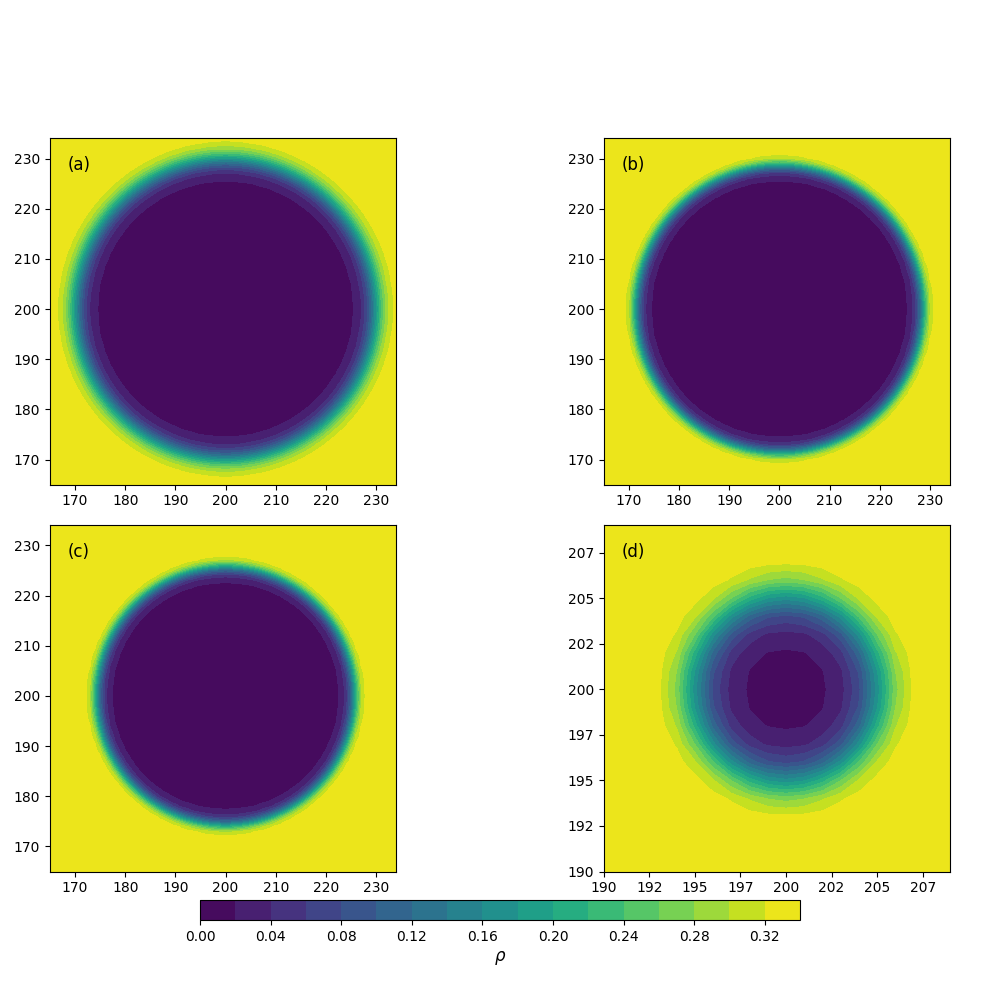
\includegraphics[scale=0.4]{contour.png}
	\caption{density contour of bubble with domain size 400 and initial radius=30. (a) iteration=0, (b) iteration=100, (c) iteration=200, (d) iteration=500}
	\label{fig:con}
\end{figure}

The discrepancy observed in the final stages of collapse can be attributed to significant diffusion effects, particularly when the bubble diminishes to a minimal size. As illustrated in Figure \ref{fig:con}(d), which shows a close-up contour, pronounced diffusion is evident during the imminent collapse phase of the bubble. Furthermore, the choice of pressure averaging strategy contributes marginally to the variations in outcomes. For the purposes of this study, a centred-pressure averaging strategy was employed to maintain methodological simplicity. In the modified R-P equation, the parameter $R_{\infty}$ is adjusted due to the original formulation's assumption of an infinite boundary, which impacts the outcomes. It is conceivable that in existing literature, this parameter has been fine-tuned to align the results of the R-P equation with those obtained from LBM simulations. However, there is no universally optimized parameter that is applicable across all cases. The selection of the parameter in this article is based on an area-weighted length within a quarter of a square domain. The average length, $L_{avg}$, can be calculated using an integral that accounts for the variation of length within this domain. Given that the minimum length is half the domain length (0.5×domain) and the maximum length within the quarter of the square domain, considering the geometry and the angle at $45^\circ$, is (half domain × $\sqrt{2}$). To calculate $L_{avg}$, we integral over the angle from 0 to $\pi/4$, considering the length as a function of the angle $\alpha$, which is represented by $L(\alpha)=\frac{half domain}{cos\alpha}$, the integral formula to find
$L_{avg}$ is $L_{avg} = \frac{1}{\pi/4} \int_{0}^{\pi/4} \left( \frac{\text{half domain}}{\cos(\alpha)} \right) d\alpha$.
%\newpage
\subsection{The impact of radius}
In the analysis of radius-related outcomes depicted in Figure \ref{fig:radius}, a discernible trend is observed, whereby an increase in the radius correlates with a rise in the specific iterations required to achieve a 5\% discrepancy. This pattern is particularly pronounced when comparing a radius of 350 (l.u.) with one of 35 (l.u.), where the iterations necessary to reach the 5\% difference threshold are significantly more extended for the larger radius. Notably, the relationship between the radius and the number of iterations appears to be almost linear. Furthermore, towards the end of the simulation, the radius difference consistently remains substantial, potentially attributable to the inadequate resolution when dealing with smaller bubbles. This observation underscores the pivotal role of radius in impacting the outcomes of simulations. The fundamental cause of this phenomenon is the resolution insufficiency encountered at smaller radii, resulting in diminished simulation precision. This conclusion is in concordance with the findings presented by Ezzatneshan and Vaseghnia \cite{ezzatneshan2021dynamics}, who reported a decreasing discrepancy with increasing radius in the initial phases of their study. Similarly, the research by Peng et al. \cite{peng2019simulation} on a growth case showed a marked deviation towards the end of the simulation, especially pronounced at smaller radii.

Furthermore, the study conducted by Gai et al. \cite{gai2022lbm} also provides empirical evidence in support of this observation. Their findings, particularly in the context of the collapse case simulations, reveal discernible discrepancies between the results obtained from the LBM and those predicted by the R-P equation towards the end of the simulation. This outcome further corroborates the assertion that adequate resolution, particularly in terms of the radius, is imperative for the accuracy of LBM simulations. Additionally, the research conducted by Peng et al. \cite{peng2018single} provides further evidence of this phenomenon. Particularly in the collapse case simulations, their findings exhibit certain discrepancies. This observation lends credence to the theory that when the bubble diminishes in size, the resolution employed in the simulation may not be sufficiently large to accurately capture the complexities of the process. 
\setlength{\abovecaptionskip}{10pt} % Set the space above the caption
\begin{figure}[htp]
	\centering
	\pgfplotsset{yticklabel style={text width=1.1em, align=left}}
	\pgfplotsset{xticklabel style={text width=2em, align=left}}
	\setlength\figureheight{0.8\textwidth}
	\setlength\figurewidth{0.8\textwidth}
	% This file was created by matlab2tikz.
%
%The latest updates can be retrieved from
%  http://www.mathworks.com/matlabcentral/fileexchange/22022-matlab2tikz-matlab2tikz
%where you can also make suggestions and rate matlab2tikz.
%
\definecolor{mycolor1}{rgb}{0.92900,0.69400,0.12500}%
\definecolor{mycolor2}{rgb}{0.30100,0.74500,0.93300}%
\definecolor{mycolor3}{rgb}{0.85000,0.32500,0.09800}%
\definecolor{mycolor4}{rgb}{0.46600,0.67400,0.18800}%
\definecolor{mycolor5}{rgb}{0.00000,0.44700,0.74100}%
%
\begin{tikzpicture}

\begin{axis}[%
width=0.951\figurewidth,
height=0.419\figureheight,
at={(0\figurewidth,0.581\figureheight)},
scale only axis,
xmin=0,
xmax=1000,
xlabel style={font=\color{white!15!black}},
xlabel={t [t.u.]},
ymin=0,
ymax=40,
ytick={10, 20, 30, 40},
ylabel style={font=\color{white!15!black}},
ylabel={R [l.u.]},
axis background/.style={fill=white}
]
\addplot [color=black, forget plot]
  table[row sep=crcr]{%
0	19.9377145796532\\
1	19.9592432253339\\
2	19.9944015675611\\
3	20.0329341437323\\
4	20.0692388741157\\
5	20.1010277655497\\
6	20.1271634184779\\
7	20.1474795503083\\
8	20.1623472198139\\
9	20.1723525804473\\
10	20.1780918385672\\
11	20.1802499929369\\
12	20.1794762618731\\
13	20.1762190975984\\
14	20.1709284476655\\
15	20.1638921151116\\
16	20.1553981195014\\
17	20.1456124870564\\
18	20.1347416913988\\
19	20.1228702457204\\
20	20.1100421506484\\
21	20.0964226358066\\
22	20.0820552778654\\
23	20.0669433229253\\
24	20.0511705873389\\
25	20.0347803787375\\
26	20.017775784897\\
27	20.00024000288\\
28	19.9804191891946\\
29	19.9605180952077\\
30	19.9405373177186\\
31	19.9204377715405\\
32	19.9003391017783\\
33	19.8802019033305\\
34	19.8600265329954\\
35	19.8398527089335\\
36	19.819680546389\\
37	19.799470958136\\
38	19.7792634202302\\
39	19.7590970882995\\
40	19.7388939113408\\
41	19.7186931238945\\
42	19.698456035016\\
43	19.6782217184597\\
44	19.6579902850212\\
45	19.6377232809137\\
46	19.6174210545933\\
47	19.5970839539077\\
48	19.5767123260854\\
49	19.5562682728882\\
50	19.5357523804314\\
51	19.515127150811\\
52	19.4944694190258\\
53	19.4736657617903\\
54	19.4527550937039\\
55	19.4317004875414\\
56	19.4105030231858\\
57	19.3891637841443\\
58	19.3676088362779\\
59	19.3458772001099\\
60	19.3238955427503\\
61	19.3016657337528\\
62	19.2791896571003\\
63	19.2563950487957\\
64	19.233321344563\\
65	19.2098969389029\\
66	19.186087784026\\
67	19.1618969511506\\
68	19.1372543015763\\
69	19.1121635542508\\
70	19.0865556210861\\
71	19.060434921004\\
72	19.0336972576249\\
73	19.0063842444677\\
74	18.9764123194869\\
75	18.946139913454\\
76	18.9162501938916\\
77	18.8866686560624\\
78	18.8574639728151\\
79	18.828562175678\\
80	18.7999255522948\\
81	18.7715520882413\\
82	18.7434397960714\\
83	18.7155516876749\\
84	18.6878162912907\\
85	18.6602674389529\\
86	18.6328344081373\\
87	18.6055165356528\\
88	18.5782786481701\\
89	18.5510859805733\\
90	18.5239384857051\\
91	18.496733476868\\
92	18.4695059222471\\
93	18.4422223615635\\
94	18.4147819137378\\
95	18.3871863375851\\
96	18.3594373934005\\
97	18.3314024256112\\
98	18.3031179361404\\
99	18.2745198369913\\
100	18.2455448940755\\
101	18.2161307481001\\
102	18.186249013396\\
103	18.1558388269876\\
104	18.1248731258881\\
105	18.0931944258487\\
106	18.060843369142\\
107	18.0276652551005\\
108	17.9929899311228\\
109	17.9556101406104\\
110	17.9188669542048\\
111	17.8827535148552\\
112	17.847231269777\\
113	17.8122305900123\\
114	17.777714568126\\
115	17.743646887232\\
116	17.7099604359484\\
117	17.6766203715979\\
118	17.6435612469763\\
119	17.6107185877613\\
120	17.5780906677917\\
121	17.5455834257401\\
122	17.5131348511384\\
123	17.480683844352\\
124	17.4482006543075\\
125	17.4155953172947\\
126	17.382809444428\\
127	17.3498156582086\\
128	17.3164670943834\\
129	17.2827386919041\\
130	17.2485463787539\\
131	17.2138075393034\\
132	17.1784410564741\\
133	17.142337974907\\
134	17.1053914483306\\
135	17.0674968297125\\
136	17.0285517727574\\
137	16.987388562731\\
138	16.9437822249558\\
139	16.9010847116168\\
140	16.8592839862091\\
141	16.8182552069318\\
142	16.7779323211766\\
143	16.7382505850019\\
144	16.6991186205192\\
145	16.6604745236354\\
146	16.6222022755795\\
147	16.5842704828179\\
148	16.5465387950149\\
149	16.5089511533153\\
150	16.4714253712659\\
151	16.4338537387017\\
152	16.3961305131989\\
153	16.3581786803857\\
154	16.3198960749018\\
155	16.2811295196416\\
156	16.2418080380708\\
157	16.2017572425905\\
158	16.1609109582289\\
159	16.1190748295811\\
160	16.0761365828564\\
161	16.0318842113195\\
162	15.9850891088792\\
163	15.9360010199041\\
164	15.888223172338\\
165	15.8416092540345\\
166	15.7960415119971\\
167	15.7514050253283\\
168	15.7075628773742\\
169	15.6644548456425\\
170	15.621900029213\\
171	15.5798185262738\\
172	15.538059700333\\
173	15.4965001154489\\
174	15.4550428259237\\
175	15.4134979083883\\
176	15.3717740410703\\
177	15.329711433512\\
178	15.2871538988357\\
179	15.2439489144784\\
180	15.1999246083739\\
181	15.1548905589578\\
182	15.108661493461\\
183	15.0610121602612\\
184	15.0117466917863\\
185	14.9592659189028\\
186	14.9076174943873\\
187	14.857472268528\\
188	14.8086719582988\\
189	14.7610626784243\\
190	14.7144730085064\\
191	14.6687359363494\\
192	14.6237313913018\\
193	14.5792572160034\\
194	14.5351372407658\\
195	14.4912414936412\\
196	14.4473596005594\\
197	14.4033277448422\\
198	14.3589449047284\\
199	14.3140151385024\\
200	14.2683273097212\\
201	14.2216356587604\\
202	14.1737015472013\\
203	14.1242738357714\\
204	14.0730503899642\\
205	14.0197004831189\\
206	13.9649981286903\\
207	13.9119014926079\\
208	13.8603788595957\\
209	13.8102090589447\\
210	13.7611775164377\\
211	13.7130758291954\\
212	13.6656827375096\\
213	13.618764478449\\
214	13.5721120242126\\
215	13.5254671020064\\
216	13.4785784951976\\
217	13.4312020254253\\
218	13.3830468915197\\
219	13.333813350614\\
220	13.2831937048288\\
221	13.2308034273073\\
222	13.1762721690779\\
223	13.1191586945912\\
224	13.058990069944\\
225	12.9956711419426\\
226	12.9374976550786\\
227	12.8808214872712\\
228	12.8253305408314\\
229	12.7707559904424\\
230	12.7167894684636\\
231	12.6631167729313\\
232	12.6094341264247\\
233	12.5553849418246\\
234	12.5006094047085\\
235	12.4447298435822\\
236	12.3873218238597\\
237	12.3279024813602\\
238	12.2659804259484\\
239	12.200939716377\\
240	12.1321531174781\\
241	12.0588714102247\\
242	11.983424527194\\
243	11.9167779892344\\
244	11.8516973408347\\
245	11.7877544092095\\
246	11.7245527376244\\
247	11.6616307857723\\
248	11.5985195649627\\
249	11.5347438018054\\
250	11.469757689899\\
251	11.4029506275044\\
252	11.333679388344\\
253	11.2611978536157\\
254	11.1846564409081\\
255	11.1031045390602\\
256	11.0154237963997\\
257	10.9367190499053\\
258	10.8626579837821\\
259	10.7902102580371\\
260	10.7187914348281\\
261	10.6477675890473\\
262	10.5764705260208\\
263	10.5041906468586\\
264	10.4301280506821\\
265	10.3534244986872\\
266	10.2730789855951\\
267	10.1879680097804\\
268	10.0967776134247\\
269	9.99830028895088\\
270	9.91424180835771\\
271	9.83274500742372\\
272	9.75295758438746\\
273	9.67408023682148\\
274	9.59517938187854\\
275	9.51529107275391\\
276	9.43342829651152\\
277	9.34832805152798\\
278	9.25857343900452\\
279	9.16279538561624\\
280	9.0589556835888\\
281	8.95575855274942\\
282	8.86430521575719\\
283	8.77523978342708\\
284	8.68749348437989\\
285	8.5999312005504\\
286	8.51121778504068\\
287	8.41984726397063\\
288	8.32417673892052\\
289	8.22226424712837\\
290	8.11187903565982\\
291	7.99188024966634\\
292	7.88861278744133\\
293	7.78882926107377\\
294	7.69076953840001\\
295	7.59289912074228\\
296	7.49327478587967\\
297	7.38989062961868\\
298	7.28024578109757\\
299	7.16142569662768\\
300	7.02982755832999\\
301	6.90789019217751\\
302	6.79504776918582\\
303	6.68444729647529\\
304	6.57375755982119\\
305	6.46015698181466\\
306	6.34055099388137\\
307	6.21106439010453\\
308	6.06685676151186\\
309	5.92290743680258\\
310	5.79370919056089\\
311	5.66716726644187\\
312	5.53955240416574\\
313	5.4066620890261\\
314	5.26318559571366\\
315	5.10230113781315\\
316	4.93252308420803\\
317	4.78166899374558\\
318	4.63331912448802\\
319	4.48141110672929\\
320	4.31833001541644\\
321	4.13382002174389\\
322	3.93077125662826\\
323	3.74844907919348\\
324	3.56635924649962\\
325	3.37235143948821\\
326	3.14909054265128\\
327	2.89505148849072\\
328	2.65595784463709\\
329	2.40010176431481\\
330	2.08668507122899\\
331	1.69290098899276\\
332	1.20235372765726\\
};
\addplot [color=black, dashed, forget plot]
  table[row sep=crcr]{%
99	18.2745198369913\\
119	17.6419340178207\\
139	16.9149699658174\\
159	16.0827965087088\\
179	15.1305974198407\\
199	14.0373730200434\\
219	12.771800268035\\
239	11.2835320836879\\
259	9.48153807653868\\
279	7.16175415963012\\
299	3.56526511043855\\
};
\addplot[only marks, mark=*, mark options={}, mark size=2.5000pt, color=black, fill=black, forget plot] table[row sep=crcr]{%
x	y\\
223	13.1762721690779\\
};
\node[right, align=left, inner sep=0]
at (rel axis cs:0.05,0.95) {(a)};
\addplot [color=black, forget plot]
  table[row sep=crcr]{%
0	24.9340494392332\\
1	24.9543958415995\\
2	24.9885677302634\\
3	25.0271544625919\\
4	25.0634104283838\\
5	25.0952364222223\\
6	25.121525379021\\
7	25.142052597174\\
8	25.157169415926\\
9	25.167489643578\\
10	25.1736351484363\\
11	25.1762336354481\\
12	25.1759801009053\\
13	25.1733182964712\\
14	25.1686931659447\\
15	25.1624867582413\\
16	25.1548912428277\\
17	25.1460988342269\\
18	25.1363647789257\\
19	25.1256912705811\\
20	25.114143783496\\
21	25.1019137699058\\
22	25.0889402933399\\
23	25.0753514310503\\
24	25.0611492040579\\
25	25.046335721084\\
26	25.0309758325928\\
27	25.0151341561645\\
28	24.9985625826515\\
29	24.980078387486\\
30	24.9614345835684\\
31	24.9427563741214\\
32	24.9239197350089\\
33	24.9051115250894\\
34	24.886207814767\\
35	24.8672709413505\\
36	24.8483011216523\\
37	24.8293602218752\\
38	24.8104481759359\\
39	24.7915034559356\\
40	24.7725876454151\\
41	24.7537006782514\\
42	24.7347813074311\\
43	24.7159519225303\\
44	24.697090188834\\
45	24.6783181232633\\
46	24.6594529546957\\
47	24.6406773229383\\
48	24.621869637049\\
49	24.6030906402462\\
50	24.5842798281067\\
51	24.5654374121786\\
52	24.5465636038283\\
53	24.5276586142363\\
54	24.5087226543927\\
55	24.4896959604247\\
56	24.4706389039111\\
57	24.4514321203793\\
58	24.4321957702983\\
59	24.4128108666304\\
60	24.3933376916097\\
61	24.3736579254605\\
62	24.3538912647463\\
63	24.3339197808001\\
64	24.3138036757608\\
65	24.2934847303302\\
66	24.272905126923\\
67	24.2521250924612\\
68	24.2310870307953\\
69	24.2097337655578\\
70	24.1881255653974\\
71	24.1662054949118\\
72	24.1439170608161\\
73	24.1212624103895\\
74	24.0981856476026\\
75	24.0747472753405\\
76	24.0508338424093\\
77	24.0263905874212\\
78	24.001478491075\\
79	23.9738014297975\\
80	23.9463028105776\\
81	23.9191532619745\\
82	23.8922935407184\\
83	23.8656649451567\\
84	23.8393797946953\\
85	23.8133226014626\\
86	23.7874920609245\\
87	23.761830421321\\
88	23.7364494544177\\
89	23.7111788723912\\
90	23.6861303495125\\
91	23.6611906784373\\
92	23.6363593388438\\
93	23.6116915651954\\
94	23.5870195913785\\
95	23.5624546422748\\
96	23.5379408067865\\
97	23.5134226373125\\
98	23.4889003201537\\
99	23.464318983338\\
100	23.4396791576717\\
101	23.4149265473754\\
102	23.3901167400726\\
103	23.3650864858676\\
104	23.3399463181235\\
105	23.3145884042563\\
106	23.2889601013536\\
107	23.2630633732372\\
108	23.2369001975137\\
109	23.2103648205142\\
110	23.183406245146\\
111	23.1560812500579\\
112	23.1282856620819\\
113	23.0999697390396\\
114	23.0710843178919\\
115	23.041580836778\\
116	23.0114113588929\\
117	22.9786803803431\\
118	22.9451999788904\\
119	22.9122894647002\\
120	22.8798396580837\\
121	22.8478992499035\\
122	22.8164123016969\\
123	22.785323517416\\
124	22.7546299983389\\
125	22.7242256152016\\
126	22.6941598848952\\
127	22.6643790753387\\
128	22.6348300237439\\
129	22.6054601228381\\
130	22.5762682783112\\
131	22.5472025685773\\
132	22.5181608967632\\
133	22.4892445188089\\
134	22.4602509708443\\
135	22.4312314521755\\
136	22.4021362677145\\
137	22.3729162425135\\
138	22.3434728012906\\
139	22.313857798247\\
140	22.2838742743813\\
141	22.2536245591001\\
142	22.2229629876551\\
143	22.1918440534735\\
144	22.1601737357621\\
145	22.1279571248703\\
146	22.0951017368959\\
147	22.0615163321405\\
148	22.0271109681796\\
149	21.9909749038994\\
150	21.9522100387457\\
151	21.9142058839643\\
152	21.8769552528757\\
153	21.8403080357045\\
154	21.8043063505042\\
155	21.7688496469093\\
156	21.7338859536068\\
157	21.6993639916414\\
158	21.6652331504065\\
159	21.6314434662225\\
160	21.5979456034142\\
161	21.5645978310327\\
162	21.5314455997261\\
163	21.4983951448024\\
164	21.4653538456255\\
165	21.4322761505917\\
166	21.3990712803064\\
167	21.3657408891139\\
168	21.3321501100739\\
169	21.2982565247209\\
170	21.2639730883157\\
171	21.2291688780384\\
172	21.1938495448621\\
173	21.1578864964021\\
174	21.1211530459871\\
175	21.0835689422163\\
176	21.0450553590181\\
177	21.0054908353044\\
178	20.961811771315\\
179	20.9186202914801\\
180	20.8763037251676\\
181	20.8348959505296\\
182	20.7942574578604\\
183	20.7543802119437\\
184	20.7150847246965\\
185	20.6763225092785\\
186	20.6380458247169\\
187	20.600165213325\\
188	20.5625925316664\\
189	20.5252409150152\\
190	20.4879827737041\\
191	20.450817828205\\
192	20.4135374414897\\
193	20.3761436110602\\
194	20.3385142308584\\
195	20.3005290317866\\
196	20.2620696083139\\
197	20.2230603557236\\
198	20.1833862474443\\
199	20.1428531142865\\
200	20.101391418314\\
201	20.0588526737448\\
202	20.0150513185916\\
203	19.9672935731272\\
204	19.9190886618555\\
205	19.8721031441642\\
206	19.826203500118\\
207	19.7813370996999\\
208	19.7372965824871\\
209	19.6940722811841\\
210	19.6515002937899\\
211	19.6094580337989\\
212	19.5678633067341\\
213	19.5265590492909\\
214	19.4854667646136\\
215	19.4443958334549\\
216	19.4033094284561\\
217	19.3620588838935\\
218	19.3204607543481\\
219	19.2784091456773\\
220	19.2357631308128\\
221	19.1923476271541\\
222	19.147990992785\\
223	19.1025616535177\\
224	19.055822125334\\
225	19.0076125488258\\
226	18.9545072870603\\
227	18.9021266782726\\
228	18.8512074198352\\
229	18.8015515040301\\
230	18.753070815346\\
231	18.7055392713444\\
232	18.6588747205834\\
233	18.6128927785699\\
234	18.5674471802546\\
235	18.5223945010715\\
236	18.4775599273462\\
237	18.4328059707545\\
238	18.3879301626412\\
239	18.3428349218228\\
240	18.2972572411396\\
241	18.2510727067983\\
242	18.2040270948739\\
243	18.1559706817385\\
244	18.1066590860121\\
245	18.0558539786977\\
246	18.0032910015951\\
247	17.9452669358457\\
248	17.8887356420536\\
249	17.8338632963043\\
250	17.7804646035401\\
251	17.7283589921782\\
252	17.6773390655051\\
253	17.627233370468\\
254	17.5778125818467\\
255	17.5288832173213\\
256	17.4802866067792\\
257	17.4317763851725\\
258	17.3831418290542\\
259	17.334206977365\\
260	17.2847102909708\\
261	17.2344261108449\\
262	17.1830753580953\\
263	17.1304155667512\\
264	17.0761236516266\\
265	17.0199439703444\\
266	16.958666641794\\
267	16.8973150166439\\
268	16.8379932479647\\
269	16.7804098782917\\
270	16.7243657284297\\
271	16.6695560563831\\
272	16.6157946420709\\
273	16.5627903664186\\
274	16.5103412522433\\
275	16.4581420074325\\
276	16.4059757125936\\
277	16.3535506829243\\
278	16.3006093167763\\
279	16.2468217155019\\
280	16.1919195844506\\
281	16.1355385235982\\
282	16.0773255047476\\
283	16.0168625528957\\
284	15.9511257506999\\
285	15.8862544183645\\
286	15.8236360816879\\
287	15.7630001402907\\
288	15.7040601277054\\
289	15.6464894753889\\
290	15.5899955880312\\
291	15.5342701533854\\
292	15.4790135534243\\
293	15.4239107634219\\
294	15.368655626849\\
295	15.3128569809784\\
296	15.256228355226\\
297	15.1983537143257\\
298	15.1388306464432\\
299	15.0772255492633\\
300	15.0130538503229\\
301	14.9445110305436\\
302	14.8779413690087\\
303	14.8138930614688\\
304	14.7520040597515\\
305	14.6919034389338\\
306	14.6332540698738\\
307	14.575665925737\\
308	14.5187822226223\\
309	14.4622362088116\\
310	14.4056101208054\\
311	14.3485403947283\\
312	14.2905730805617\\
313	14.2312492617539\\
314	14.1700863808466\\
315	14.1065012632372\\
316	14.0399351916592\\
317	13.9704803749677\\
318	13.9030429590124\\
319	13.8382064577374\\
320	13.7754898219793\\
321	13.7144863376287\\
322	13.6547106020635\\
323	13.5957124561198\\
324	13.537038691564\\
325	13.4781606623707\\
326	13.4186040894538\\
327	13.357786988714\\
328	13.2951143113929\\
329	13.2299282144095\\
330	13.161462185803\\
331	13.0889024431745\\
332	13.0112781759229\\
333	12.9376817744289\\
334	12.8674956765215\\
335	12.7991808524254\\
336	12.7321387191978\\
337	12.6657952599528\\
338	12.5995204622512\\
339	12.5327103740763\\
340	12.4646471445363\\
341	12.3945994251385\\
342	12.3217049296677\\
343	12.2450429005078\\
344	12.1635116544687\\
345	12.0758799995653\\
346	11.9837691830185\\
347	11.9026647685884\\
348	11.8238809287895\\
349	11.7466436902316\\
350	11.6701774450481\\
351	11.5936383387707\\
352	11.5161467894134\\
353	11.4367274490608\\
354	11.3542948755796\\
355	11.2676183297108\\
356	11.1752570867893\\
357	11.0755585681075\\
358	10.972624399386\\
359	10.8826954260031\\
360	10.7954754003502\\
361	10.709917597894\\
362	10.62491500068\\
363	10.539329087389\\
364	10.451865501214\\
365	10.361126710363\\
366	10.2654754608942\\
367	10.1630250853948\\
368	10.0515443192692\\
369	9.94292759560125\\
370	9.84562066792691\\
371	9.75096046960626\\
372	9.65773004712972\\
373	9.56434412510162\\
374	9.46915894930212\\
375	9.37031484257871\\
376	9.26577962269745\\
377	9.15306673500957\\
378	9.02918231724935\\
379	8.91472177153351\\
380	8.80909803645205\\
381	8.70609949330501\\
382	8.60377877964002\\
383	8.50007650068851\\
384	8.39264133208003\\
385	8.2788310290587\\
386	8.15534297294873\\
387	8.01815309861527\\
388	7.89459141542129\\
389	7.77877173194353\\
390	7.66530224286744\\
391	7.55161529051064\\
392	7.43466785621352\\
393	7.31101038163474\\
394	7.17638109454164\\
395	7.02558013727984\\
396	6.8870523415978\\
397	6.75817231987781\\
398	6.63147563595851\\
399	6.50317680186771\\
400	6.36881826577079\\
401	6.22293025339772\\
402	6.05858653176214\\
403	5.89730434218519\\
404	5.751125782872\\
405	5.60717269531184\\
406	5.45970735968552\\
407	5.30172093861667\\
408	5.12413210012554\\
409	4.93201221166224\\
410	4.76176871137015\\
411	4.59430031103413\\
412	4.42051472473455\\
413	4.22854436588749\\
414	4.00148855374199\\
415	3.7944472059588\\
416	3.59217337265566\\
417	3.3784240327572\\
418	3.13007659297423\\
419	2.85144810792161\\
420	2.58718155029093\\
421	2.29426731426185\\
422	1.91333730031934\\
423	1.46419958797424\\
};
\addplot [color=black, dashed, forget plot]
  table[row sep=crcr]{%
99	23.464318983338\\
119	22.9363073001712\\
139	22.3397557166287\\
159	21.6700194043737\\
179	20.9212737419127\\
199	20.086137890174\\
219	19.1550967068751\\
239	18.1155939399133\\
259	16.9505978640895\\
279	15.6359692697886\\
299	14.1355823737612\\
319	12.3911403978062\\
339	10.2940346304812\\
359	7.59395986229556\\
379	3.25588687057345\\
399	-18.7554328233551\\
419	-29.3505058430337\\
};
\addplot[only marks, mark=*, mark options={}, mark size=2.5000pt, color=black, fill=black, forget plot] table[row sep=crcr]{%
x	y\\
290	15.6464894753889\\
};
\addplot [color=black, forget plot]
  table[row sep=crcr]{%
0	29.9340254080008\\
1	29.9532130811672\\
2	29.9864461263509\\
3	30.0246201885546\\
4	30.0606322953397\\
5	30.0922930628237\\
6	30.1185768370073\\
7	30.1392735832281\\
8	30.154542027893\\
9	30.1650025640252\\
10	30.1713734009172\\
11	30.1742866798629\\
12	30.1743777288953\\
13	30.1721016679138\\
14	30.1679146127345\\
15	30.1620910774502\\
16	30.1549966829504\\
17	30.146724106225\\
18	30.1374569411084\\
19	30.127378556537\\
20	30.116490585585\\
21	30.1048854208061\\
22	30.0925647291067\\
23	30.0797112347721\\
24	30.0662359177268\\
25	30.0523210910195\\
26	30.0377875367212\\
27	30.0228173411793\\
28	30.0074118307222\\
29	29.9906729007279\\
30	29.9730542242524\\
31	29.9552767717797\\
32	29.9375203949358\\
33	29.9196955371782\\
34	29.9018024806535\\
35	29.8839308127234\\
36	29.8660804950601\\
37	29.8482514894277\\
38	29.8303547724093\\
39	29.8125683825787\\
40	29.7947144176623\\
41	29.7768818244891\\
42	29.7590705647081\\
43	29.7413690547003\\
44	29.7236002413556\\
45	29.7058526470885\\
46	29.6881262339127\\
47	29.6703329308058\\
48	29.6526488711237\\
49	29.6348980559507\\
50	29.6171684802246\\
51	29.5994601058477\\
52	29.5816853869432\\
53	29.5639320029564\\
54	29.5461126179629\\
55	29.5283147009668\\
56	29.5103640398508\\
57	29.4924351903737\\
58	29.4744412382802\\
59	29.4564692297722\\
60	29.4383458004728\\
61	29.420071549614\\
62	29.4018199726563\\
63	29.3833320110834\\
64	29.3648672854823\\
65	29.3461673905388\\
66	29.3274052871446\\
67	29.3084094619269\\
68	29.2893524417069\\
69	29.2699774913873\\
70	29.2505425975652\\
71	29.2307917159936\\
72	29.2108968329546\\
73	29.1906881704736\\
74	29.1702521768301\\
75	29.1495048956593\\
76	29.1284477158928\\
77	29.1070820441322\\
78	29.0854093044224\\
79	29.0633464699659\\
80	29.0408110517711\\
81	29.0179737329302\\
82	28.9940794089847\\
83	28.9682102860321\\
84	28.9427223524645\\
85	28.9174464738066\\
86	28.8924651340177\\
87	28.8676935867532\\
88	28.8432140570288\\
89	28.8189421142729\\
90	28.794876815517\\
91	28.7711000054665\\
92	28.7474450708193\\
93	28.7239115073734\\
94	28.700581186769\\
95	28.6773709733387\\
96	28.6542803764026\\
97	28.6313908843378\\
98	28.6084560874503\\
99	28.5856397180312\\
100	28.562941297443\\
101	28.5401974410859\\
102	28.5174897764799\\
103	28.4948182173072\\
104	28.4721016112362\\
105	28.4493402597994\\
106	28.4265344643304\\
107	28.4036038492564\\
108	28.3806296526495\\
109	28.3574513457029\\
110	28.3342305839685\\
111	28.31072721765\\
112	28.2871027783592\\
113	28.2631982069827\\
114	28.239015023156\\
115	28.2145547602186\\
116	28.1898189649826\\
117	28.1647298720758\\
118	28.1392103012021\\
119	28.1133417485936\\
120	28.08696848923\\
121	28.0601722333372\\
122	28.0327983740977\\
123	28.0048504400962\\
124	27.974062449297\\
125	27.9432639967809\\
126	27.91292284589\\
127	27.8830362395822\\
128	27.8535238885748\\
129	27.8244610401897\\
130	27.7956905561362\\
131	27.7673650158968\\
132	27.7392510402219\\
133	27.7114243117868\\
134	27.6838832736746\\
135	27.656549900713\\
136	27.6294231252746\\
137	27.6024257011706\\
138	27.5756330675961\\
139	27.5488923967812\\
140	27.5222792850813\\
141	27.4956419407524\\
142	27.469056108294\\
143	27.4424463294356\\
144	27.4157377300866\\
145	27.3890060529703\\
146	27.3621018472155\\
147	27.3351010031982\\
148	27.3077805328294\\
149	27.2802913535117\\
150	27.2525603780475\\
151	27.2244410141649\\
152	27.1960098014419\\
153	27.1671212631625\\
154	27.1377048557495\\
155	27.1078376891111\\
156	27.077376310545\\
157	27.0463249453664\\
158	27.0145419279198\\
159	26.9802855053812\\
160	26.9450267564116\\
161	26.9103669497637\\
162	26.8763018208695\\
163	26.8428271939314\\
164	26.8098671034888\\
165	26.7773463649752\\
166	26.7453336079188\\
167	26.7137541105789\\
168	26.6824626845759\\
169	26.6515285984228\\
170	26.6208078882778\\
171	26.5903700315894\\
172	26.5601427873276\\
173	26.5299841881294\\
174	26.4999642250483\\
175	26.4700121232656\\
176	26.4399878376056\\
177	26.4099618376051\\
178	26.3797951872702\\
179	26.3494890834067\\
180	26.3189754549235\\
181	26.2882559845215\\
182	26.25712552744\\
183	26.2256560347857\\
184	26.1937129850093\\
185	26.1613001119704\\
186	26.1282846519843\\
187	26.094603375076\\
188	26.0601938357217\\
189	26.0249944046262\\
190	25.9877285945577\\
191	25.948212557378\\
192	25.9094877953358\\
193	25.8715477653451\\
194	25.8343193431883\\
195	25.7977968681475\\
196	25.7618420747557\\
197	25.72638446538\\
198	25.6914203501741\\
199	25.6568802772996\\
200	25.6226955588182\\
201	25.5887982476791\\
202	25.555186425085\\
203	25.5216627873739\\
204	25.4882919530913\\
205	25.454943477298\\
206	25.4215529009805\\
207	25.3881208982317\\
208	25.3545195698859\\
209	25.3206223808981\\
210	25.28643205915\\
211	25.2518875785965\\
212	25.2168014504704\\
213	25.1811785798822\\
214	25.1449606984264\\
215	25.1079012054303\\
216	25.0700708480202\\
217	25.0312264550026\\
218	24.9904411562577\\
219	24.9466142455146\\
220	24.9038710577172\\
221	24.8620158122421\\
222	24.8211019079981\\
223	24.780936521153\\
224	24.7414518283933\\
225	24.7026419475563\\
226	24.6643794565451\\
227	24.6265991897849\\
228	24.5891763363603\\
229	24.5520478863142\\
230	24.5151515894399\\
231	24.4783660201114\\
232	24.4416906806278\\
233	24.4048868345397\\
234	24.3680155175523\\
235	24.330900243309\\
236	24.2934257131335\\
237	24.2555369326933\\
238	24.2171210202189\\
239	24.1780081673312\\
240	24.1381474454599\\
241	24.0973726634585\\
242	24.0555780074284\\
243	24.0126018134317\\
244	23.9656428544039\\
245	23.9184667306087\\
246	23.8724447531947\\
247	23.8275646799243\\
248	23.7836449387214\\
249	23.7406194877249\\
250	23.6983671825011\\
251	23.6567686746532\\
252	23.6157063339686\\
253	23.5751197616084\\
254	23.5348940106048\\
255	23.4948604992658\\
256	23.4550179665438\\
257	23.4151458529435\\
258	23.3751358679772\\
259	23.3348812137872\\
260	23.2943308586989\\
261	23.2532723167468\\
262	23.2115500673135\\
263	23.1690646648595\\
264	23.1256648628648\\
265	23.0812019766741\\
266	23.0354769380323\\
267	22.9871318036163\\
268	22.9355693984459\\
269	22.8854947157393\\
270	22.8367333423158\\
271	22.7891140959786\\
272	22.7426239984717\\
273	22.6969928754139\\
274	22.6522115354122\\
275	22.6080154457962\\
276	22.5643478790641\\
277	22.5211022728296\\
278	22.4780726401395\\
279	22.4351064545801\\
280	22.3921036485694\\
281	22.3489157423528\\
282	22.3053468146849\\
283	22.261303176688\\
284	22.2165446608089\\
285	22.1708843078915\\
286	22.12423643729\\
287	22.0763222613218\\
288	22.0269168924426\\
289	21.9736272525715\\
290	21.9187209987923\\
291	21.8654270427229\\
292	21.813628718951\\
293	21.7631645382292\\
294	21.7137819545444\\
295	21.6654209049646\\
296	21.6178355790662\\
297	21.5708775895839\\
298	21.5244011373494\\
299	21.4781706612484\\
300	21.4320924151825\\
301	21.3859827714523\\
302	21.3395701783775\\
303	21.2927238504058\\
304	21.2452702717058\\
305	21.1969044040808\\
306	21.1475059688836\\
307	21.096779365662\\
308	21.0444353251891\\
309	20.9893101443435\\
310	20.9300475949282\\
311	20.8726870453668\\
312	20.8170266624477\\
313	20.7629555651988\\
314	20.7101510805521\\
315	20.6584253321875\\
316	20.6076367780372\\
317	20.5575199407943\\
318	20.5078986171524\\
319	20.4585162665663\\
320	20.4092045512526\\
321	20.3597154526168\\
322	20.3098057773274\\
323	20.2592782429533\\
324	20.2078171920026\\
325	20.1551950015116\\
326	20.101108576138\\
327	20.0452622020522\\
328	19.9860497372834\\
329	19.9228983832568\\
330	19.8618804831204\\
331	19.8028428961262\\
332	19.7454807530926\\
333	19.6894966380185\\
334	19.6347157482201\\
335	19.5808522761762\\
336	19.5276648427828\\
337	19.4748414261037\\
338	19.4221898519058\\
339	19.3694095041819\\
340	19.3162062970833\\
341	19.2623298173161\\
342	19.2074248221392\\
343	19.151181340621\\
344	19.0932245783261\\
345	19.0332263031574\\
346	18.968277452788\\
347	18.901626484959\\
348	18.8373937335526\\
349	18.7752527149015\\
350	18.7148861947771\\
351	18.6559854931057\\
352	18.5982153152583\\
353	18.5413174718543\\
354	18.4849717179933\\
355	18.4287975762445\\
356	18.3725587462566\\
357	18.3158569531572\\
358	18.2583705499786\\
359	18.1996869653842\\
360	18.1394378588208\\
361	18.0772004924229\\
362	18.0124357856664\\
363	17.9411458651041\\
364	17.8713761317049\\
365	17.8041754352231\\
366	17.7391143924531\\
367	17.6759017361271\\
368	17.6140997345555\\
369	17.5533754263276\\
370	17.4933131810365\\
371	17.4335693838628\\
372	17.3737493072217\\
373	17.3134090621846\\
374	17.2521470296978\\
375	17.1894848483286\\
376	17.1249591141601\\
377	17.0580348461536\\
378	16.9870134282341\\
379	16.911174058259\\
380	16.8384468890127\\
381	16.7684511652397\\
382	16.7006803857189\\
383	16.6347003175564\\
384	16.570063198221\\
385	16.5063351314234\\
386	16.443068342325\\
387	16.3797480794745\\
388	16.3159019675346\\
389	16.2510461610966\\
390	16.1846343081878\\
391	16.116035455278\\
392	16.0446426136081\\
393	15.9676304196134\\
394	15.8890057613535\\
395	15.8137519549751\\
396	15.7414126658555\\
397	15.671377482738\\
398	15.6031799280693\\
399	15.5362491765788\\
400	15.4700577033152\\
401	15.404095640949\\
402	15.3377526511305\\
403	15.2704861206552\\
404	15.2016344797393\\
405	15.1305158295457\\
406	15.0563861661924\\
407	14.9774364919249\\
408	14.8968467844411\\
409	14.8200841780781\\
410	14.7465220327786\\
411	14.6754954447262\\
412	14.6064510851863\\
413	14.5387085846713\\
414	14.4716962564616\\
415	14.4047593324835\\
416	14.3372053345874\\
417	14.2683273097212\\
418	14.1973862611893\\
419	14.1235157950339\\
420	14.045752634632\\
421	13.9641400882534\\
422	13.8853404130056\\
423	13.8100374113913\\
424	13.7375091697874\\
425	13.6670087974536\\
426	13.5977830174568\\
427	13.5290719462517\\
428	13.4600733843201\\
429	13.389963954217\\
430	13.3178136411702\\
431	13.2426301452584\\
432	13.1632466358032\\
433	13.0783918809343\\
434	12.9879406970628\\
435	12.9045745426296\\
436	12.8242285585311\\
437	12.7459815106792\\
438	12.6689082188275\\
439	12.5920637259161\\
440	12.514438533458\\
441	12.4349496695412\\
442	12.3523736938909\\
443	12.2653335066834\\
444	12.1722618496969\\
445	12.0712736280092\\
446	11.9669902540831\\
447	11.8742704745077\\
448	11.7843649759245\\
449	11.6960705881252\\
450	11.6081596075513\\
451	11.5192775109145\\
452	11.4279575839926\\
453	11.3325748063263\\
454	11.2311975713658\\
455	11.1215777515061\\
456	11.0010274959681\\
457	10.8969497258327\\
458	10.7969323755735\\
459	10.6992036582717\\
460	10.6021153340515\\
461	10.5038927426504\\
462	10.4025906611783\\
463	10.2959572923692\\
464	10.1813916740651\\
465	10.0557288492827\\
466	9.93285390758473\\
467	9.82279674668972\\
468	9.71600128251217\\
469	9.61030224400557\\
470	9.50353531513723\\
471	9.39302286261765\\
472	9.27583552088454\\
473	9.14862862056978\\
474	9.00698040981761\\
475	8.88273019595303\\
476	8.76477960961672\\
477	8.64924708304142\\
478	8.53322410806475\\
479	8.41354243790806\\
480	8.28658319315197\\
481	8.14770153339743\\
482	7.99283841677857\\
483	7.85866968439583\\
484	7.72994658606909\\
485	7.60294385986254\\
486	7.47378569666893\\
487	7.33783387144115\\
488	7.18948609553389\\
489	7.02163365328577\\
490	6.86841490720771\\
491	6.72531138191698\\
492	6.58397197861526\\
493	6.43885980670543\\
494	6.28326201830943\\
495	6.10873549175321\\
496	5.92410042535041\\
497	5.76096599877868\\
498	5.60136225129952\\
499	5.43741266155912\\
500	5.25933795453828\\
501	5.05410418530368\\
502	4.85276704777064\\
503	4.66768422182702\\
504	4.48052762693335\\
505	4.27708679064516\\
506	4.03719059980541\\
507	3.8038723420442\\
508	3.58266277828333\\
509	3.34753805313882\\
510	3.06702366822165\\
511	2.77079690889897\\
512	2.48038019267593\\
513	2.13544258115216\\
514	1.69116602515102\\
515	1.13675116516994\\
};
\addplot [color=black, dashed, forget plot]
  table[row sep=crcr]{%
99	28.5856397180312\\
119	28.1038666943028\\
139	27.5667638675475\\
159	26.9716865360082\\
179	26.3154554220109\\
199	25.5942425396347\\
219	24.8033900370332\\
239	23.9371914781213\\
259	22.9885421170667\\
279	21.948469150633\\
299	20.8053753902121\\
319	19.5438659493555\\
339	18.1427986175415\\
359	16.5715940373682\\
379	14.7835099370922\\
399	12.6979496138565\\
419	10.1605447665603\\
439	6.74140981598178\\
};
\addplot[only marks, mark=*, mark options={}, mark size=2.5000pt, color=black, fill=black, forget plot] table[row sep=crcr]{%
x	y\\
323	20.3098057773274\\
};
\addplot [color=black, forget plot]
  table[row sep=crcr]{%
0	34.9340096557603\\
1	34.9523250286609\\
2	34.9848515592748\\
3	35.0228348883472\\
4	35.0585653333894\\
5	35.0901817671416\\
6	35.1165518355422\\
7	35.1371578958464\\
8	35.1525974254238\\
9	35.1631040581738\\
10	35.1696584322773\\
11	35.1727509663713\\
12	35.172998392594\\
13	35.1710190802779\\
14	35.1670611238689\\
15	35.1614967545938\\
16	35.1546982496476\\
17	35.1469141009419\\
18	35.1380221510092\\
19	35.1282708811224\\
20	35.1177850510613\\
21	35.1066892285656\\
22	35.0949845757543\\
23	35.0825492383579\\
24	35.0696307518578\\
25	35.0563530875883\\
26	35.0424714754282\\
27	35.0281100583218\\
28	35.0133926226782\\
29	34.9979526197717\\
30	34.9809353902123\\
31	34.96381245411\\
32	34.9467062729338\\
33	34.9294948147165\\
34	34.9123003016423\\
35	34.895000942165\\
36	34.8778403641247\\
37	34.8605751297685\\
38	34.8434483863999\\
39	34.8262171762903\\
40	34.8091241676268\\
41	34.7919268812865\\
42	34.7748675077548\\
43	34.7578248553205\\
44	34.7407988994115\\
45	34.7237896155035\\
46	34.7067969791204\\
47	34.6899413046193\\
48	34.6729817724135\\
49	34.6560388147635\\
50	34.6392323946101\\
51	34.6223223961417\\
52	34.6054288996858\\
53	34.5885518810984\\
54	34.5716913162826\\
55	34.5547277778546\\
56	34.5379001647458\\
57	34.5208505937586\\
58	34.5039368992002\\
59	34.4869208352732\\
60	34.469802729319\\
61	34.4525829101408\\
62	34.4353802871222\\
63	34.4180763737115\\
64	34.4006715011077\\
65	34.3831660019255\\
66	34.3655602101798\\
67	34.3478544612711\\
68	34.3300490919702\\
69	34.3120267084816\\
70	34.2939056300305\\
71	34.2755687173739\\
72	34.2571340481655\\
73	34.2383675146369\\
74	34.2196215309859\\
75	34.2005451566898\\
76	34.1811395308297\\
77	34.161639212096\\
78	34.1418114279471\\
79	34.1217737862885\\
80	34.1014107753638\\
81	34.0807236019235\\
82	34.0597134896901\\
83	34.0383816791814\\
84	34.016613714138\\
85	33.9938335185997\\
86	33.9693528498589\\
87	33.9451378681775\\
88	33.9211875129325\\
89	33.8975007372706\\
90	33.873961763072\\
91	33.8507992173695\\
92	33.8277827579791\\
93	33.8049118536923\\
94	33.7823001016847\\
95	33.7598325512305\\
96	33.7375086874085\\
97	33.7154416722859\\
98	33.6934035054617\\
99	33.6716208844861\\
100	33.6498664100304\\
101	33.6282531131355\\
102	33.6066675628445\\
103	33.5852225020991\\
104	33.5638047929113\\
105	33.5424143829873\\
106	33.5210512201663\\
107	33.4996030297041\\
108	33.4782943478596\\
109	33.4569008203632\\
110	33.435422824357\\
111	33.4139723866932\\
112	33.3924379485022\\
113	33.3707085268834\\
114	33.3488961515374\\
115	33.3270012031047\\
116	33.3049131407865\\
117	33.2826327893842\\
118	33.2601609791791\\
119	33.2374985458594\\
120	33.2145360095392\\
121	33.1913848441499\\
122	33.1678258821812\\
123	33.1439707802754\\
124	33.1198208880086\\
125	33.0952680385758\\
126	33.0702047376375\\
127	33.0447425814553\\
128	33.0188834994733\\
129	32.9916498134322\\
130	32.962396498075\\
131	32.9337373205111\\
132	32.9053444860514\\
133	32.8774329300368\\
134	32.8498924166023\\
135	32.8226134677748\\
136	32.7957024511508\\
137	32.7691576688021\\
138	32.7427630308011\\
139	32.7167319910749\\
140	32.6908491774982\\
141	32.665220686231\\
142	32.6398454176921\\
143	32.6145095430055\\
144	32.5893191765331\\
145	32.5643797788227\\
146	32.5393726408955\\
147	32.514509599909\\
148	32.4895789675462\\
149	32.4647919331485\\
150	32.4399374558006\\
151	32.4150159319803\\
152	32.3900277582538\\
153	32.3648685824511\\
154	32.3396438758416\\
155	32.3142496146526\\
156	32.2886866899576\\
157	32.2628519070572\\
158	32.2367466675263\\
159	32.2102686336404\\
160	32.1836269016501\\
161	32.1565121760633\\
162	32.1289269580975\\
163	32.100976832725\\
164	32.0724580973335\\
165	32.0433739109258\\
166	32.0137274863461\\
167	31.9817831763028\\
168	31.9487797163587\\
169	31.9163536204316\\
170	31.8845015814713\\
171	31.8531188981369\\
172	31.8222029874684\\
173	31.7917513122045\\
174	31.7617613802391\\
175	31.7320293584736\\
176	31.7027549694068\\
177	31.6737351885696\\
178	31.6449687664158\\
179	31.6164544675631\\
180	31.5880912895838\\
181	31.5599781604951\\
182	31.5319150277954\\
183	31.504001008128\\
184	31.476037292809\\
185	31.448222074765\\
186	31.4202585258872\\
187	31.3922461152095\\
188	31.364185236878\\
189	31.3359780898841\\
190	31.3075275819318\\
191	31.2789330130371\\
192	31.2499023440552\\
193	31.2206330919978\\
194	31.1910294599273\\
195	31.1608993035539\\
196	31.1302458355514\\
197	31.0991690302035\\
198	31.0673820449172\\
199	31.0349857394241\\
200	31.001791903572\\
201	30.9650250042577\\
202	30.9288234984829\\
203	30.8932791671172\\
204	30.8584829969759\\
205	30.8242401824795\\
206	30.7905473019783\\
207	30.7574009996155\\
208	30.7246091829712\\
209	30.6923582166512\\
210	30.6604569021288\\
211	30.6289032708606\\
212	30.5975081389372\\
213	30.5664575920967\\
214	30.5355632437318\\
215	30.5047312838221\\
216	30.4740543900923\\
217	30.4433464544157\\
218	30.4126078507106\\
219	30.3818389519481\\
220	30.3509480118611\\
221	30.3197521057068\\
222	30.2883450448268\\
223	30.2566367932806\\
224	30.2245380934966\\
225	30.1920516404851\\
226	30.1589982387145\\
227	30.1253818392148\\
228	30.0910253516889\\
229	30.0560244295367\\
230	30.0201134760289\\
231	29.9816811927912\\
232	29.9417333868292\\
233	29.9026072083225\\
234	29.8642966360856\\
235	29.8267068332985\\
236	29.7898327300892\\
237	29.7535808434545\\
238	29.7178586499771\\
239	29.6826626535707\\
240	29.6479015215303\\
241	29.6134847964369\\
242	29.5793228701409\\
243	29.5455015496616\\
244	29.5117574841817\\
245	29.4781773053409\\
246	29.4446734585713\\
247	29.4110726806428\\
248	29.3774621985505\\
249	29.3435840253529\\
250	29.3095261821997\\
251	29.2751187837945\\
252	29.2403645688654\\
253	29.2050957050986\\
254	29.1692311282367\\
255	29.1326906661772\\
256	29.095395071822\\
257	29.057266059951\\
258	29.0181421424675\\
259	28.9759325903904\\
260	28.9325062494213\\
261	28.8901279543767\\
262	28.8487890720787\\
263	28.808232240445\\
264	28.7684513654945\\
265	28.7293579563084\\
266	28.6909468586282\\
267	28.6530488276605\\
268	28.6155783208379\\
269	28.5785323780483\\
270	28.54182661982\\
271	28.5052962840496\\
272	28.4688593382129\\
273	28.4325154246396\\
274	28.3961029188354\\
275	28.3595422769876\\
276	28.3227547844214\\
277	28.2856625633599\\
278	28.2481087891166\\
279	28.2100179415714\\
280	28.1713154032301\\
281	28.1318483468319\\
282	28.0915447259529\\
283	28.0502548365652\\
284	28.0077525459047\\
285	27.9609999972039\\
286	27.9146370399319\\
287	27.8694372603228\\
288	27.8253126869513\\
289	27.7821766224097\\
290	27.7398666267213\\
291	27.698375767245\\
292	27.6575442866428\\
293	27.6172143620562\\
294	27.5773821342688\\
295	27.5379679733432\\
296	27.4987419325566\\
297	27.4596274826936\\
298	27.4206241482469\\
299	27.3815065304893\\
300	27.3422013206283\\
301	27.3026360695125\\
302	27.2625905458789\\
303	27.2220694761657\\
304	27.1807820998241\\
305	27.1387359319578\\
306	27.0956449169925\\
307	27.0515196191146\\
308	27.0060790683983\\
309	26.955921676874\\
310	26.9065294074913\\
311	26.8584719678128\\
312	26.8115922600295\\
313	26.7658072165969\\
314	26.7210350660143\\
315	26.6770529326084\\
316	26.6337828228081\\
317	26.5910770981689\\
318	26.5488605229064\\
319	26.5069885675358\\
320	26.465248482218\\
321	26.423639644972\\
322	26.3819526338422\\
323	26.3400500460951\\
324	26.2977962446747\\
325	26.2550573804279\\
326	26.2116327226023\\
327	26.167461285241\\
328	26.1222783851207\\
329	26.0759592693516\\
330	26.0283135995336\\
331	25.9771297349813\\
332	25.923928823261\\
333	25.8723509946625\\
334	25.8221781523715\\
335	25.7732623022224\\
336	25.7254579131509\\
337	25.678621777012\\
338	25.6325471831112\\
339	25.5872268563533\\
340	25.5423274679635\\
341	25.497845432061\\
342	25.4535180579984\\
343	25.4092799772333\\
344	25.3648737082938\\
345	25.3201735951102\\
346	25.2750557946857\\
347	25.2292710002144\\
348	25.1826370753893\\
349	25.1349748147552\\
350	25.0861080659363\\
351	25.0357385167326\\
352	24.9820753609285\\
353	24.9254728362197\\
354	24.8707343581734\\
355	24.817529117166\\
356	24.7657776578013\\
357	24.7152188903361\\
358	24.6657178587197\\
359	24.6171419005911\\
360	24.5691794385451\\
361	24.5217642918973\\
362	24.4746516033344\\
363	24.4277195990923\\
364	24.3806700295738\\
365	24.3333868667844\\
366	24.2856969387879\\
367	24.2372536283169\\
368	24.1879500470456\\
369	24.1375648093615\\
370	24.0857065782882\\
371	24.032222403799\\
372	23.9747210541205\\
373	23.9150918578678\\
374	23.8574090376637\\
375	23.801476643611\\
376	23.7471028534519\\
377	23.6939874137539\\
378	23.6420033287941\\
379	23.5909146669435\\
380	23.5404896421846\\
381	23.4904452613899\\
382	23.4407230994262\\
383	23.3909374152079\\
384	23.3409269148896\\
385	23.290424607731\\
386	23.2392222297104\\
387	23.1870616196163\\
388	23.1335825591294\\
389	23.0785385746233\\
390	23.021582733813\\
391	22.9593710969069\\
392	22.8968656480614\\
393	22.8364725870983\\
394	22.7779536741978\\
395	22.7210760701627\\
396	22.6655092146628\\
397	22.6110825960236\\
398	22.5574764499946\\
399	22.5044783911999\\
400	22.451779191242\\
401	22.399125538139\\
402	22.3462688434912\\
403	22.2929155343723\\
404	22.2387777567745\\
405	22.183524296505\\
406	22.1268309952649\\
407	22.0682836833731\\
408	22.0076234407599\\
409	21.9405542622818\\
410	21.8752324243445\\
411	21.8122013091683\\
412	21.7510935362275\\
413	21.6916916482649\\
414	21.6336897123152\\
415	21.5766954427862\\
416	21.520463809036\\
417	21.4647087990281\\
418	21.4090586008752\\
419	21.3532402474413\\
420	21.2969411203469\\
421	21.2397199755318\\
422	21.1812799847495\\
423	21.1211976563919\\
424	21.059104482641\\
425	20.9938928765622\\
426	20.9227782101819\\
427	20.8545354443684\\
428	20.7886809789806\\
429	20.724916115902\\
430	20.6628220042524\\
431	20.6021174856352\\
432	20.5424437701958\\
433	20.4833664822481\\
434	20.4245445837171\\
435	20.3656447864968\\
436	20.306258998211\\
437	20.2459477735531\\
438	20.1843232398261\\
439	20.120845799874\\
440	20.0551114462543\\
441	19.9852109439015\\
442	19.9105617565894\\
443	19.838986783267\\
444	19.7700349534218\\
445	19.7032687722893\\
446	19.6382631920033\\
447	19.5746430074482\\
448	19.5119286175603\\
449	19.4497282872958\\
450	19.3875849660911\\
451	19.325015846513\\
452	19.261624872151\\
453	19.196842503345\\
454	19.130115392856\\
455	19.0609435548279\\
456	18.9875100159115\\
457	18.9086673549422\\
458	18.8332074647301\\
459	18.7606349349287\\
460	18.6904708503417\\
461	18.6221819983091\\
462	18.555251043269\\
463	18.4892438823714\\
464	18.4236028460782\\
465	18.3578196050499\\
466	18.2913333833296\\
467	18.2235667164777\\
468	18.1539271482904\\
469	18.081711253153\\
470	18.0062409631178\\
471	17.9228493028908\\
472	17.8426775435629\\
473	17.7658075714319\\
474	17.6916313276331\\
475	17.619592987402\\
476	17.5490627923016\\
477	17.479492185793\\
478	17.4102285092492\\
479	17.3406695926156\\
480	17.2701728571601\\
481	17.1980579952912\\
482	17.1235222400307\\
483	17.045793524303\\
484	16.9612841727473\\
485	16.8751877364636\\
486	16.7930342493934\\
487	16.7141627458027\\
488	16.6378554469843\\
489	16.5634213403121\\
490	16.4901669134695\\
491	16.4173958726667\\
492	16.3443559669975\\
493	16.2702951594245\\
494	16.1944106611044\\
495	16.1158536487098\\
496	16.0336064390963\\
497	15.9438012892158\\
498	15.8550970966146\\
499	15.7706568005438\\
500	15.6895970127007\\
501	15.6111694795392\\
502	15.5345597350425\\
503	15.4589371980676\\
504	15.383526704264\\
505	15.3074423253842\\
506	15.2298102213348\\
507	15.1496329243942\\
508	15.0658452767822\\
509	14.976202813729\\
510	14.8847400156885\\
511	14.798175089048\\
512	14.7155556667398\\
513	14.6359740533452\\
514	14.5585201555432\\
515	14.4822802060539\\
516	14.4062949746521\\
517	14.3296038151137\\
518	14.2511653890497\\
519	14.1698052785359\\
520	14.0842888349617\\
521	13.9931965078579\\
522	13.9026177238912\\
523	13.8168111905117\\
524	13.7347166939988\\
525	13.655232685165\\
526	13.5772716472625\\
527	13.4997401300025\\
528	13.4214316104242\\
529	13.3411245500706\\
530	13.2574125507925\\
531	13.1687069383283\\
532	13.0732283814559\\
533	12.9723559095567\\
534	12.8794942995358\\
535	12.7901607851112\\
536	12.7030422515888\\
537	12.6168318630519\\
538	12.5300878735063\\
539	12.441323607536\\
540	12.34883482569\\
541	12.2507132977818\\
542	12.1446771094697\\
543	12.0280638786416\\
544	11.918297685705\\
545	11.8165457637093\\
546	11.7174363655325\\
547	11.6192465848129\\
548	11.520126813556\\
549	11.4180407327185\\
550	11.3106690147616\\
551	11.1953122988342\\
552	11.0686934182228\\
553	10.9414936451805\\
554	10.8286282943394\\
555	10.7193429471547\\
556	10.6113630720321\\
557	10.5022600863706\\
558	10.3893621243337\\
559	10.2695552871778\\
560	10.1391496903504\\
561	9.99460291442621\\
562	9.8699145265402\\
563	9.75039001560062\\
564	9.63326172608784\\
565	9.51538161437964\\
566	9.39337579139191\\
567	9.26337631539944\\
568	9.12059247368709\\
569	8.96667981779707\\
570	8.8329859025545\\
571	8.70435653044349\\
572	8.5769913629697\\
573	8.44687338981476\\
574	8.30909846281678\\
575	8.15807077942208\\
576	7.98875183741292\\
577	7.84159968633601\\
578	7.70071924717769\\
579	7.56097929803868\\
580	7.41702206564065\\
581	7.2622696044968\\
582	7.0884783872294\\
583	6.91018146136518\\
584	6.75201209960568\\
585	6.5973940293584\\
586	6.4391085698096\\
587	6.26841346455212\\
588	6.07407947325583\\
589	5.87861828955722\\
590	5.70268482401515\\
591	5.52803820980011\\
592	5.34353592459202\\
593	5.13473545842918\\
594	4.90677134445535\\
595	4.70431055976591\\
596	4.50273991723964\\
597	4.28458193191799\\
598	4.02482512134848\\
599	3.77565082781144\\
600	3.53646805862049\\
601	3.27568134171908\\
602	2.95648060548723\\
603	2.65055131467345\\
604	2.32461911115864\\
605	1.89801941673863\\
606	1.3947195916261\\
};
\addplot [color=black, dashed, forget plot]
  table[row sep=crcr]{%
99	33.6716208844861\\
119	33.2163053437774\\
139	32.713865767638\\
159	32.162573676388\\
179	31.5604061797659\\
199	30.9049943139715\\
219	30.1935610890028\\
239	29.4228144823746\\
259	28.5888545087057\\
279	27.6869941461059\\
299	26.711540890562\\
319	25.6555384393951\\
339	24.5102219279714\\
359	23.2644927453871\\
379	21.9038140083032\\
399	20.408359458236\\
419	18.7508815568255\\
439	16.8892381123243\\
459	14.7568482611524\\
479	12.2343447442575\\
499	9.03605491182307\\
519	3.98580106201764\\
};
\addplot[only marks, mark=*, mark options={}, mark size=2.5000pt, color=black, fill=black, forget plot] table[row sep=crcr]{%
x	y\\
347	25.2750557946857\\
};
\end{axis}

\begin{axis}[%
width=0.951\figurewidth,
height=0.419\figureheight,
at={(0\figurewidth,0\figureheight)},
scale only axis,
clip=false,
xmode=log,
xmin=0,
xmax=3700,
xminorticks=true,
xlabel style={font=\color{white!15!black}},
xlabel={t [t.u.]},
ymode=log,
ymin=1,
ymax=1000,
yminorticks=true,
ylabel style={font=\color{white!15!black}},
ylabel={R [l.u.]},
axis background/.style={fill=white},
legend style={at={(0.97,0.03)}, anchor=south east, legend columns=3, legend cell align=left, align=left, draw=white!15!black}
]
\addplot [color=black, forget plot]
  table[row sep=crcr]{%
0	19.9377145796532\\
20	20.1100421506484\\
40	19.7388939113408\\
60	19.3238955427503\\
80	18.7999255522948\\
100	18.2455448940755\\
120	17.5780906677917\\
140	16.8592839862091\\
160	16.0761365828564\\
180	15.1999246083739\\
200	14.2683273097212\\
220	13.2831937048288\\
240	12.1321531174781\\
260	10.7187914348281\\
280	9.0589556835888\\
300	7.02982755832999\\
320	4.31833001541644\\
340	0\\
360	0\\
380	0\\
400	0\\
420	0\\
440	0\\
460	0\\
480	0\\
500	0\\
520	0\\
540	0\\
560	0\\
580	0\\
600	0\\
620	0\\
640	0\\
660	0\\
680	0\\
700	0\\
720	0\\
740	0\\
760	0\\
780	0\\
800	0\\
820	0\\
840	0\\
860	0\\
880	0\\
900	0\\
920	0\\
940	0\\
960	0\\
980	0\\
};
\addplot [color=black, dashed, forget plot]
  table[row sep=crcr]{%
99	18.2745198369913\\
139	16.9149699658174\\
179	15.1305974198407\\
219	12.771800268035\\
259	9.48153807653868\\
299	3.56526511043855\\
};
\addplot[only marks, mark=*, mark options={}, mark size=2.5000pt, color=black, fill=black, forget plot] table[row sep=crcr]{%
x	y\\
223	13.1762721690779\\
};
\node[right, align=left, inner sep=0]
at (rel axis cs:0.05,0.95) {(b)};
\addplot [color=black, forget plot]
  table[row sep=crcr]{%
0	24.9340494392332\\
20	25.114143783496\\
40	24.7725876454151\\
60	24.3933376916097\\
80	23.9463028105776\\
100	23.4396791576717\\
120	22.8798396580837\\
140	22.2838742743813\\
160	21.5979456034142\\
180	20.8763037251676\\
200	20.101391418314\\
220	19.2357631308128\\
240	18.2972572411396\\
260	17.2847102909708\\
280	16.1919195844506\\
300	15.0130538503229\\
320	13.7754898219793\\
340	12.4646471445363\\
360	10.7954754003502\\
380	8.80909803645205\\
400	6.36881826577079\\
420	2.58718155029093\\
440	0\\
460	0\\
480	0\\
500	0\\
520	0\\
540	0\\
560	0\\
580	0\\
600	0\\
620	0\\
640	0\\
660	0\\
680	0\\
700	0\\
720	0\\
740	0\\
760	0\\
780	0\\
800	0\\
820	0\\
840	0\\
860	0\\
880	0\\
900	0\\
920	0\\
940	0\\
960	0\\
980	0\\
};
\addplot [color=black, dashed, forget plot]
  table[row sep=crcr]{%
99	23.464318983338\\
139	22.3397557166287\\
179	20.9212737419127\\
219	19.1550967068751\\
259	16.9505978640895\\
299	14.1355823737612\\
339	10.2940346304812\\
379	3.25588687057345\\
419	-29.3505058430337\\
};
\addplot[only marks, mark=*, mark options={}, mark size=2.5000pt, color=black, fill=black, forget plot] table[row sep=crcr]{%
x	y\\
290	15.6464894753889\\
};
\addplot [color=black, forget plot]
  table[row sep=crcr]{%
0	29.9340254080008\\
20	30.116490585585\\
40	29.7947144176623\\
60	29.4383458004728\\
80	29.0408110517711\\
100	28.562941297443\\
120	28.08696848923\\
140	27.5222792850813\\
160	26.9450267564116\\
180	26.3189754549235\\
200	25.6226955588182\\
220	24.9038710577172\\
240	24.1381474454599\\
260	23.2943308586989\\
280	22.3921036485694\\
300	21.4320924151825\\
320	20.4092045512526\\
340	19.3162062970833\\
360	18.1394378588208\\
380	16.8384468890127\\
400	15.4700577033152\\
420	14.045752634632\\
440	12.514438533458\\
460	10.6021153340515\\
480	8.28658319315197\\
500	5.25933795453828\\
520	0\\
540	0\\
560	0\\
580	0\\
600	0\\
620	0\\
640	0\\
660	0\\
680	0\\
700	0\\
720	0\\
740	0\\
760	0\\
780	0\\
800	0\\
820	0\\
840	0\\
860	0\\
880	0\\
900	0\\
920	0\\
940	0\\
960	0\\
980	0\\
};
\addplot [color=black, dashed, forget plot]
  table[row sep=crcr]{%
99	28.5856397180312\\
139	27.5667638675475\\
179	26.3154554220109\\
219	24.8033900370332\\
259	22.9885421170667\\
299	20.8053753902121\\
339	18.1427986175415\\
379	14.7835099370922\\
419	10.1605447665603\\
};
\addplot[only marks, mark=*, mark options={}, mark size=2.5000pt, color=black, fill=black, forget plot] table[row sep=crcr]{%
x	y\\
323	20.3098057773274\\
};
\addplot [color=black]
  table[row sep=crcr]{%
0	34.9340096557603\\
20	35.1177850510613\\
40	34.8091241676268\\
60	34.469802729319\\
80	34.1014107753638\\
100	33.6498664100304\\
120	33.2145360095392\\
140	32.6908491774982\\
160	32.1836269016501\\
180	31.5880912895838\\
200	31.001791903572\\
220	30.3509480118611\\
240	29.6479015215303\\
260	28.9325062494213\\
280	28.1713154032301\\
300	27.3422013206283\\
320	26.465248482218\\
340	25.5423274679635\\
360	24.5691794385451\\
380	23.5404896421846\\
400	22.451779191242\\
420	21.2969411203469\\
440	20.0551114462543\\
460	18.6904708503417\\
480	17.2701728571601\\
500	15.6895970127007\\
520	14.0842888349617\\
540	12.34883482569\\
560	10.1391496903504\\
580	7.41702206564065\\
600	3.53646805862049\\
620	0\\
640	0\\
660	0\\
680	0\\
700	0\\
720	0\\
740	0\\
760	0\\
780	0\\
800	0\\
820	0\\
840	0\\
860	0\\
880	0\\
900	0\\
920	0\\
940	0\\
960	0\\
980	0\\
};
\addlegendentry{LBM}

\addplot [color=black, dashed]
  table[row sep=crcr]{%
99	33.6716208844861\\
139	32.713865767638\\
179	31.5604061797659\\
219	30.1935610890028\\
259	28.5888545087057\\
299	26.711540890562\\
339	24.5102219279714\\
379	21.9038140083032\\
419	18.7508815568255\\
459	14.7568482611524\\
499	9.03605491182307\\
};
\addlegendentry{R-P}

\addplot[only marks, mark=*, mark options={}, mark size=2.5000pt, color=black, fill=black, forget plot] table[row sep=crcr]{%
x	y\\
347	25.2750557946857\\
};
\addplot [color=black, forget plot]
  table[row sep=crcr]{%
0	350.00035000035\\
20	350.15844669713\\
40	349.919518510743\\
60	349.656462525569\\
80	349.412114117997\\
100	349.162011173184\\
120	348.875747902385\\
140	348.600890326674\\
160	348.344666146472\\
180	348.073067498329\\
200	347.766815394941\\
220	347.488871668885\\
240	347.217399758337\\
260	346.909040449594\\
280	346.604832364573\\
300	346.322745092607\\
320	346.02195855349\\
340	345.676281076298\\
360	345.381387397033\\
380	345.076279111498\\
400	344.73248758963\\
420	344.423779017703\\
440	344.112070419094\\
460	343.740654550954\\
480	343.420745360386\\
500	343.096722397011\\
580	341.519557117438\\
660	338.730438317187\\
740	335.617771632243\\
820	332.347369470571\\
900	328.884620697367\\
980	325.289996031462\\
1060	321.509293226121\\
1140	317.580292237385\\
1220	313.29694911431\\
1300	308.237651229098\\
1380	302.733990669738\\
1460	296.838080763705\\
1540	290.757685452521\\
1620	284.953053984356\\
1700	279.367846437082\\
1780	273.732617978758\\
1860	267.557096684432\\
1940	260.653562743222\\
2020	253.183145091665\\
2100	245.183973794737\\
2180	236.715524750975\\
2260	227.74529876767\\
2340	218.893580507964\\
2420	210.339445797628\\
2500	201.793948199493\\
2580	192.815315706157\\
2660	183.668559065054\\
2740	173.903365377927\\
2820	163.569211040267\\
2900	152.779984599778\\
2980	141.453519787933\\
3060	129.429062519414\\
3140	116.337779763276\\
3220	101.811636255531\\
3300	85.5966514589949\\
3380	66.7931283229581\\
3460	40.2918743377023\\
};
\addplot [color=black, dashed, forget plot]
  table[row sep=crcr]{%
99	349.175422240379\\
179	347.923145512224\\
259	346.117588312669\\
339	343.759969579787\\
419	340.85169323059\\
499	337.394068295232\\
579	333.388210653589\\
659	328.834928112282\\
739	323.734419279394\\
819	318.085935188234\\
899	311.887414667232\\
979	305.13536801042\\
1059	297.824321521954\\
1139	289.946333273839\\
1219	281.489884647323\\
1299	272.439683931804\\
1379	262.775367954387\\
1459	252.471085852667\\
1539	241.491056517765\\
1619	229.788668230021\\
1699	217.300818887405\\
1779	203.952237422475\\
1859	189.629465957576\\
1939	174.168330536395\\
2019	157.243727842931\\
2099	138.667982525626\\
2179	117.962368574204\\
2259	93.536152057358\\
2339	62.2835077627041\\
2419	-60.0829968315778\\
2499	-231.44500813506\\
2579	-325.266599497114\\
2659	-398.348491363961\\
2739	-459.956629829432\\
2819	-514.739313276919\\
2899	-564.739615381656\\
2979	-610.644120929182\\
3059	-653.319582796987\\
3139	-693.418052007839\\
3219	-731.37288883121\\
3299	-767.469330570424\\
3379	-801.955497251549\\
3459	-835.036782845975\\
};
\addplot[only marks, mark=*, mark options={}, mark size=2.5000pt, color=black, fill=black] table[row sep=crcr]{%
x	y\\
863	330.542453219979\\
};
\addlegendentry{5\% difference}

\end{axis}

\begin{axis}[%
width=1.227\figurewidth,
height=1.227\figureheight,
at={(-0.16\figurewidth,-0.135\figureheight)},
scale only axis,
xmin=0,
xmax=1,
ymin=0,
ymax=1,
axis line style={draw=none},
ticks=none,
axis x line*=bottom,
axis y line*=left
]
\end{axis}
\end{tikzpicture}% % Adjust the width as needed
	\caption{The impact of radius with domain size 1000 (l.u.) and initial condition from LBM at time 100. (a) radius from 20 to 35, (b) log-log plot radius including 20,25 30,35,350 }
	\label{fig:radius}
\end{figure}
\newpage
\section{Conclusions}
This article performed the LBM simulation of a single bubble based on the
Shan-Chen Model. Then validate the results with R-P equation. Based on the provided results and discussion, the following conclusion can be drawn,
\begin{itemize}
	\item Incorporating the initial conditions derived directly from the LBM at the inception point (t=0 t.u.) into the R-P equation reveals a substantial discrepancy between the two models. This significant variance underscores the sensitivity of the R-P equation to the initial state provided by LBM simulations. As the investigation progresses, applying initial conditions from subsequent time steps within the LBM framework demonstrates an improvement in the congruence between the models. Specifically, when initial conditions from the LBM at time 100 (t.u.) are employed, as opposed to those at the very start, a notable enhancement in alignment is observed. However, extending this approach to initiate the R-P equation with conditions from LBM at time 150 (t.u.) yields only a marginal further reduction in the difference between the two models. This observation suggests that while advancing the point of initial condition extraction from the LBM simulations contributes to diminishing the discrepancy with the R-P equation, the benefits of this strategy exhibit diminishing returns. Consequently, the selection of the initial condition at time 100 (t.u.) is deemed optimal for subsequent analyses, balancing improvement in model agreement against the diminishing returns observed with later initial conditions
	\item The domain size and the parameter \(R_{\infty}\) play pivotal roles in aligning the results between the LBM and the R-P equation. The parameter \(R_{\infty}\) defines the distance from the center of the bubble to the domain boundary. Notably, in LBM, the domain is square, whereas it is cylindrical in the context of the R-P equation. This discrepancy leads to a difference in the influence of the boundary of domain between LBM and the R-P equation. However, there is no established methodology for determining the optimal value of \(R_{\infty}\). It has been observed that there is no universally optimal \(R_{\infty}\) that is applicable across all domain sizes, as each domain size uniquely influences the outcomes. The literature suggests that authors may fine-tune $R_{\infty}$ to achieve congruence between the LBM and R-P equation results.
	\item An analysis of the simulation data reveals an approximately linear relationship between the radius and the iteration at which the difference between the LBM and the R-P equation reaches a 5\% threshold. Furthermore, a consistent observation towards the end of the simulation is the presence of a significant discrepancy. This is largely attributed to the insufficient resolution within the bubble when it becomes exceedingly small, thereby impacting the accuracy of the simulation.  
\end{itemize}
This study serves as a foundational
exploration preceding future endeavours in simulating bubble cluster dynamics.
\section*{Acknowledgements}
This project was financially supported by the Centre for Computational Engineering Sciences at Cranfield University under project code 15124. Furthermore, we would like to acknowledge the IT support for using the High-Performance Computing (HPC) facilities at Cranfield University, UK.
%\appendix
%\section{some appendix}\label{app:A}
\section*{Data Availability}
Data supporting this study will be available from \url{https://github.com/xiongxin9000/SINGLE-BUBBLE.git}
%\section*{References}

{\begingroup
\singlespacing
\footnotesize
\bibliography{mybibliography}
\endgroup}

\end{document}